\renewcommand{\asydir}{background/asy/}


\begin{Filesave}{\answerbodyfilename}
  \def\asydir{background/asy/} % Graphics from correct directory for this chapter
\end{Filesave}

\chapteropen[这是哈勃深场图像。它来源于将哈勃望远镜指向天空最暗的部分——即背景深处——持续 11 天。它所覆盖的天空区域，大约相当于在 75 英尺外观看一枚一角硬币的宽度。图中的每一个斑点都是一个星系，其中有成千上万个——背景中内容丰富。致谢：Robert Williams 及哈勃深场团队（STScI）与 NASA。（另参见 \citetext{深场影片}{https://www.youtube.com/watch?v=yDiD8F9ItX0}。）]{background/pix/hubble.jpg}{背景}% https://www.nationalgeographic.com/science/phenomena/2015/04/24/when-hubble-stared-at-nothing-for-100-hours/


\begin{credit}
图片来源：Robert Williams 及哈勃深场团队（STScI）与 NASA。
\end{credit}

% See also https://i.imgur.com/Ym0Dke5.gifv

% Here we will develop the ideas surrounding the definition of
% mechanical computation.
% We will see several results that are a theme throughout the subject.

% The first chapter began by saying that we are more interested in what
% things can be computed than in the details of
% how they are computed.
我们希望理解那些有效的、机械可计算的函数集合，
也就是我们定义为可由 Turing 机计算的函数集合。
本章的主要结果（也是全书最重要的结果）是：
存在任何机器都无法计算的函数——存在没有机器能完成的工作。
我们将首先用计数论证来证明这一点，然后在本章后面给出具体的不可解问题。

% ========================================================
\section{无穷}\index{infinity|(}

我们将证明，函数 $\map{f}{\N}{\N}$ 的数量多于 Turing 机的数量，因此存在没有对应机器的函数。

\subsection{势}\index{cardinality|(}
\margingraphic{0.16\textwidth}{background/pix/galileo.jpg}{\label{fig:galileo}\href{http://en.wikipedia.org/wiki/Galileo_Galilei}{Galileo Galilei 1564--1642}}\index{Galilei, Galileo!picture}\index{Galileo|see {Galilei, Galileo}}%


\begin{credit}
图片来源：File:Galilee.jpg. (2018, September 27).
\textit{Wikimedia Commons, the free media repository}.
检索于 22:19, January 26, 2020，自
\protect\url{https://commons.wikimedia.org/w/index.php?title=File:Galilee.jpg&oldid=322065651}。
\end{credit}

函数集合和 Turing 机集合都是无限的。
我们将从 \citetext{两个悖论}{%
  Quine 称这些为真实悖论：它们起初可能显得荒谬，但我们将证明它们却是真的。
  \autocite{wiki:Paradoxes}}开始，
它们突显了在比较无限集大小时直觉所面临的挑战。
然后我们将给出解决这些谜题的数学工具，并将其应用于函数集合和 Turing 机集合。

第一个谜题是
\citetext{\definend{Galileo 悖论}}{%
  他并非发明者，但
  他在其著名的《关于两门新科学的对话和数学证明》中使其广为人知。}.\index{Galileo's Paradox}\index{paradox!Galileo's}
它比较了完全平方数集合与自然数集合的大小。
前者是后者的真子集，因此可能看起来在某种意义上更小。
然而，下图表明这两个集合可以逐元素地对应起来，
所以在这个意义上，平方数的个数与自然数的个数恰好一样多。
\ifbool{MakingPaperCopy}{%


\begin{fig}{自然数与平方数之间的对应 $n\leftrightarrow n^2$。}
  \includegraphics{\asydir galileo/galileo000}
  \end{fig}


}{%


\begin{animatedfigure}{自然数与平方数之间的对应 $n\leftrightarrow n^2$。}
  \animategraphics[poster=first]{3}{\asydir galileo/galileo}{000}{012}
  \end{animatedfigure}


}
第二个谜题是
\definend{Aristotle 悖论}.\index{Aristotle's Paradox}\index{paradox!Aristotle's}
下图左侧有两个圆。
如果让它们滚动一周，那么较小圆留下的轨迹较短。
但如果将小圆放在大圆内部一起滚动（就像火车轮那样），
那么它们似乎留下了等长的轨迹。

\begin{center}
  \begin{minipage}[b]{0.5\linewidth}
    \ifbool{MakingPaperCopy}{%
      \begin{fig}{半径不同的圆，其周长也不同。} \centering
        \includegraphics{\asydir aristotle/aristotle1050}
      \end{fig}
    }{%
      \begin{animatedfigure}{半径不同的圆，其周长也不同。} \centering
        \animategraphics[poster=last]{12}{\asydir aristotle/aristotle1}{000}{050}
      \end{animatedfigure}
    }
  \end{minipage}
  \hspace{1em}
  \begin{minipage}[b]{0.45\linewidth}
    \ifbool{MakingPaperCopy}{%
      \begin{fig}{嵌套的圆一起滚动。}\centering
        \includegraphics{\asydir aristotle/aristotle2050}
      \end{fig}
    }{%
      \begin{animatedfigure}{嵌套的圆一起滚动。}\centering
        \animategraphics[poster=last]{12}{\asydir aristotle/aristotle2}{000}{050}
      \end{animatedfigure}
    }
  \end{minipage}
% \hspace*{2em}\animategraphics{12}{\asydir aristotle/aristotle1}{000}{050}
% \hspace*{\fill}
% \animategraphics{12}{\asydir aristotle/aristotle2}{000}{050}\hspace*{2em}
\end{center}


与 Galileo 悖论类似，人们可能认为小圆上的点构成的集合在某种意义上是更小的。
但是，逐点地看，小圆上的点与大圆上的点是可以对应的。
正确的看法是，这两个点集拥有相同数量的元素。

下面的动画以两种方式展示了点的匹配。
左边将它们显示为嵌套的圆，内部的点与外部的点相对应。
第二个动画将其展开，使圆周变成了线段，这样对于上方的每一个点，在底部都有一个与之匹配的点。
\ifbool{MakingPaperCopy}{%


\begin{fig}{圆周上的对应点
    $x\cdot(2\pi r_0)\leftrightarrow x\cdot(2\pi r_1)$。%
    % with $x\in\leftclosed{0}{1}$.
    }\centering
    \includegraphics{\asydir aristotle/aristotle3015}
  \end{fig}


}{%


\begin{animatedfigure}{圆周上的对应点
    $x\cdot(2\pi r_0)\leftrightarrow x\cdot(2\pi r_1)$。%
    % with $x\in\leftclosed{0}{1}$.
    }\centering
    \animategraphics[poster=2]{3}{\asydir aristotle/aristotle3}{000}{025}
  \end{animatedfigure}


}

一个\index{correspondence}\index{function!correspondence}对应被定义为一个既是一一的又是满射的函数。
函数~$\map{f}{D}{C}$ 是\index{one-to-one function}\index{function!one-to-one}一一的，如果对 $x_0,x_1\in D$，由 $f(x_0)=f(x_1)$ 能推出 $x_0=x_1$。
它是\index{onto function}\index{function!onto}满射的，如果对任意~$y\in C$，都存在~$x\in D$ 使得 $y=f(x)$。
（附录~\ref{sec:Functions} 为相关复习。）
% The sketches below show two non-correspondences.
在下图中，左边的映射是一一的但不是满射，因为存在一个陪域元素没有定义域元素与之对应。
右边的映射是满射但不是一一的，因为两个输入映射到了同一个输出。

\begin{center}
  \includegraphics{\asydir maps/maps01.pdf}
  \hspace*{5em}
  \includegraphics{\asydir maps/maps00.pdf}
\end{center}

%<*lem:OneToOneOntoFiniteSets>


\begin{lemma} \label{lem:OneToOneOntoFiniteSets}
对于一个定义域有限的函数，其定义域中的元素个数大于或等于其值域中的元素个数。
如果该函数是一一的，那么其定义域与值域有相同数量的元素；而如果它不是一一的，那么其定义域有更多的元素。
因此，两个有限集拥有相同数量的元素，当且仅当它们能对应，也就是说，当且仅当存在从一个集合到另一个集合的函数，并且该函数是一个对应。
\end{lemma}


%</lem:OneToOneOntoFiniteSets>

\begin{proof}
\zcref{exer:OneToOneOntoFiniteSets}.
\end{proof}

%<*lem:EquinumerosityIsEquivalence>


\begin{lemma} \label{lem:EquinumerosityIsEquivalence}
两个集合之间的"存在从一个到另一个的对应"这一关系是一个等价关系。
\end{lemma}


%</lem:EquinumerosityIsEquivalence>

\begin{proof}
自反性（任何集合与自身相关）是显然的，因为集合通过恒等函数与自身对应。
对于对称性，假设 $S_0$ 与~$S_1$ 相关，即存在一个对应 $\map{f}{S_0}{S_1}$，回想其逆 $\map{f^{-1}}{S_1}{S_0}$ 存在并且是反方向的一个对应。
对于传递性，假设 $S_0$ 与~$S_1$ 相关且 $S_1$ 与~$S_2$ 相关，即存在对应 $\map{f}{S_0}{S_1}$ 和 $\map{g}{S_1}{S_2}$。
同时回想，复合 $\map{\composed{g}{f}}{S_0}{S_2}$ 是一个对应。
\end{proof}

我们现在为这个关系取个名字。
这将 \zcref{lem:OneToOneOntoFiniteSets} 中关于"大小相同"集合的观察，从有限集推广到了无限集。

%<*def:Cardinality>

\begin{definition} \label{def:Cardinality}
如果两个集合之间存在一一对应，则它们具有\citetext{\definend{同势}}{%
  数有两种本性。
  第一，把昴星团称为“七姐妹”时，我们是将其视为一个集合，而不带有任何次序。
  第二则相反，提及“七宗罪”时，显然其中一些罪孽比其他的更重。
  第一种指涉关乎数的基数性质，第二种则关乎其序数性质。
  对于有限数，二者紧密相连，如\protect\zcref{lem:OneToOneOntoFiniteSets}所述，
  但对于无限数，二者却不再一致。}\index{cardinality!definition}\index{set!cardinality}，
或称\definend{等势}\index{equinumerous sets}\index{set!equinumerous}，
记作$\sizeof{S_0}=\sizeof{S_1}$。
\end{definition}


%</def:Cardinality>

\begin{example} \label{ex:PerfectSquaresCountable}
Galileo 悖论\index{Galileo's Paradox}在于，平方数的集合
$S=\set{n^2\suchthat n\in\N}$
与 $\N$ 同势，记作 $\sizeof{S}=\sizeof{\N}$。
函数 $\map{f}{\N}{S}$ 由 $f(n)=n^2$ 给出，
它是一一的，因为如果
$f(x_0)=f(x_1)$ 那么 $x_0^2=x_1^2$，且由于它们非负，可得 $x_0=x_1$。
它是满射的，因为根据 $S$ 的定义，陪域中的任意元素 $y\in S$ 都是定义域 $\N$ 中某个 $n$ 的平方。
\end{example}

\begin{example} \label{ex:RealIntervalsCorrespond}
Aristotle 悖论\index{Aristotle's Paradox}在于，对于 $r_0, r_1\in\R^+\!$，
区间 $\leftclosed{0}{2\pi r_0}$ 与区间 $\leftclosed{0}{2\pi r_1}$ 同势。
映射 $g(x)=(2\pi r_1/2\pi r_0)\cdot x$
是一个一一对应；验证留作\zcref{exer:VerifyAsParadox}。
\end{example}

\begin{example}
集合 $S_0=\set{0,1,2,3}$ 和 $S_1=\set{10,11,12,13}$
同势，即 $\sizeof{S_0}=\sizeof{S_1}$。
从 $S_0$ 到 $S_1$ 的一个对应是 $x\mapsto x+10$。
\end{example}

\begin{example}
大于零的自然数集合，
$\N^+=\set{1,2,\ldots}$，与 $\N$ 同势。
一个对应是 $\map{f}{\N}{\N^+}$，由 $n\mapsto n+1$ 给出。
\end{example}

\margingraphic[l]{.2\textwidth}{background/pix/GeorgCantor.png}{\label{fig:cantor}\href{http://en.wikipedia.org/wiki/Georg_Cantor}{Georg Cantor1845--\-1918}}\index{Cantor, G!picture} % https://upload.wikimedia.org/wikipedia/commons/6/67/Georg_Cantor3.jpg
\citetext{以这种方式比较集合大小}{%
  还有其他数学上比较无限集大小的方法。
  一种是“渐近密度”，这超出了我们的范围。}
\citetext{是由 G~Cantor 在 1870 年代提出的}{%
  由于他的发现，Cantor 被一位杰出的数学家、他以前的教授 L~Kronecker
  斥为“青年的腐蚀者”。那还是在埃尔维斯之前。}。
正如上文的悖论所生动展示的，\zcref{def:Cardinality} 引入了一个深刻的思想。
我们应当确信，它抓住了我们说集合具有“相同个数”元素时想表达的含义。
支持这一点的论据之一是，它是\zcref{lem:OneToOneOntoFiniteSets}的自然推广。
论据之二是\zcref{lem:EquinumerosityIsEquivalence}，它将集合划分成类，使得在同一类中的所有集合都具有相同的势。
也就是说，它为“等势”中的“等”字提供了依据。
最重要的支持性论据是，正如 Turing 对其机器的定义一样，Cantor 的定义本身极具说服力。
G\"odel 注意到了这一点，他写道：
“无论应用于无限集的‘数’意味着什么，我们当然希望它具有这样的性质：如果保持对象本身不变，而以任何方式改变……例如改变它们的颜色或在空间中的分布……属于某个类的对象的数量都不会改变。
然而由此立即可得，如果两个集合的元素能够建立一一对应，它们就会有相同的[势]，
\citetext{这就是 Cantor 的定义}{\autocite{Godel64}}。”

%<*def:FiniteInfinite>


\begin{definition}
如果集合与某个 $n\in\N$ 的 $\set{0,1,\ldots\, n}$ 同势，或者它是空集，那么它是\definend{有限的}\index{finite set}\index{set!finite}。
否则它是\definend{无限的}\index{infinite set}\index{set!infinite}。
\end{definition}


%</def:FiniteInfinite>

对我们而言，
\citetext{最重要的无限集是自然数集$\N=\set{0,1,2,\ldots}$}{%
  它的存在由无穷公理保证，这是数学的标准公理之一，即 Zermelo-Frankel 公理。}。

%<*def:Countable>


\begin{definition}  \label{def:Countable}
一个与自然数集同势的集合是\definend{可数无限的}\index{countably infinite set}\index{set!countably infinite}。
一个有限或可数无限的集合是\definend{可数的}\index{countable set}\index{set!countable}。
如果一个集合是某个定义域为自然数的函数的值域，
那么我们说该函数\definend{枚举}\index{enumerate}\index{function!enumeration}该集合，
或\definend{是……的一个枚举}。\footnotemark[1]
\end{definition}

\footnotetext[1]{%
  “定义域为自然数的函数”这一说法似乎暗示该函数是全函数，但在 \zcref{sec:ComputablyEnumerableSets} 中，我们将把此概念应用于一些非全函数，即那些在某些自然数上没有定义的函数。
}
%</def:Countable>

“枚举”一词背后的思想是，函数 $\map{f}{\N}{S}$ 列出了它的值域：先是 $f(0)$，然后是 $f(1)$，依此类推。
（此列表可能有重复项，即 $f(n_0)=f(n_1)$ 但 $n_0\neq n_1$。）
我们通常对可计算的枚举感兴趣。

% As always, we are particularly interested in functions that are computable
% and all the examples below are computable.\footnote{%
%   To produce noncomputable correspondences we would need
%   material that we have not yet covered.}

\begin{example} \label{ex:MultiplesOfThreeCountable}
由 3 的倍数组成的集合 $3\N=\set{3k\suchthat k\in\N}$ 是可数的。
自然的映射 $\map{g}{\N}{3\N}$ 是 $g(n)=3n$。
\end{example}

\begin{example} \label{ex:NWithGapsCountable}
集合 $\N-\set{2,5}=\set{0,1,3,4,6,7,\ldots}$ 是可数的。
下面的函数填补了空缺，同时给出了形式化定义和表格说明。
\begin{equation*}
  f(n)=\begin{cases}
         n    &\case{if $n<2$}  \\
         n+1  &\case{if $n\in\set{2,3}$} \\
         n+2  &\case{if $n\geq 4$}
       \end{cases}
  \quad
  \begin{array}{r|ccccccc@{\hspace{6pt}}c}
    n
      &0 &1 &2 &3 &4 &5 &6 &\ldots \\ \cline{2-9}
    f(n)
      &0
      &1
      &3
      &4
      &6
      &7
      &8
      &\ldots
  \end{array}
  \qquad
\end{equation*}
这个函数显然既是一一的又是满射的。
\end{example}

%<*ex:SetOfPrimesCountable>


\begin{example} \label{ex:PrimesCountable}
质数集合~$P$ 是可数的。
存在一个函数~$\map{p}{\N}{P}$，其中 $p(n)$ 是第 $n$ 个质数，即 $p(0)=2$，$p(1)=3$，依此类推。
\end{example}


%</ex:SetOfPrimesCountable>

\begin{example}  \label{ex:StringsCountable}
取定符号集 $\Sigma=\set{\str{a},\ldots\,\str{z}}$。
考虑由这些符号构成的串的集合，例如 \str{az} 和~\str{abba}。
所有此类串的集合 $\kleenestar{\Sigma}\!$,\index{Kleene star} 是可数的。
下表展示了一种对应，即把串按
\citetext{\definend{字典序（lexicographic order）}}{%
  有时也称为词典序或字母序。}\index{lexicographic order}排列，
其中较短的串排在较长的串之前，而长度相同的串则按字母顺序排列。
（第一项是空串，
$\emptystring=\text{‘$\mskip 2mu$’}$。）\index{string!empty}\index{empty string@empty string, $\emptystring$}
\begin{center}
  \begin{tabular}{r|ccc@{\hspace{6pt}}c@{\hspace{6pt}}ccc@{\hspace{6pt}}c}
    自然数 $n\in\N$  &$0$    &$1$   &$2$ &$\ldots$  &$26$  &$27$ &$28$ &$\ldots$   \\
    \cline{2-9}
    符号串 $f(n)\in\kleenestar{\Sigma}$  &$\emptystring$  &\str{a} &\str{b} &$\ldots$
    &\str{z} &\str{aa} &\str{ab}  &$\ldots$
  \end{tabular}
\end{center}
\end{example}

%<*ex:SetOfIntegersCountable>


\begin{example} \label{ex:ZIsCountable}
整数集 $\Z=\set{\ldots,-2,-1,0,1,2,\ldots}$ 是可数的。
一种自然的对应是在正数和负数之间交替。
\begin{equation*}
  \begin{array}{r|*{7}{c}@{\hspace{6pt}}c}
    n\in\N  &0    &1   &2 &3  &4  &5  &6 &\ldots
   \\ \cline{2-9}
    f(n)\in\Z  &0  &+1 &-1 &+2  &-2 &+3 &-3 &\ldots
  \end{array}
\end{equation*}
\end{example}


%</ex:SetOfIntegersCountable>

\zcref{ex:ZIsCountable} 又回到了关于无限的悖论。
我们可能会天真地以为，正数和负数合起来，会让 $\Z$ 在某种意义上是 $\N$ 的两倍大。
然而这正是 Galileo 悖论：\index{Galileo's Paradox}
衡量一个集合有多少元素的正确方法，不是看它包含或被包含，而是看它的势。

最后，我们提一下另一个悖论，
\ifbool{MakingPaperCopy}{%
  由 Zeno 提出。
}{%
  \citetext{由 Zeno 提出}{%
    Zeno 提出了一些与运动相关的悖论。
    参见 \autocite{wiki:Zeno}
    \autocite{sep:Zeno},
    \autocite{Bragg}，
    以及 \url{http://www.smbc-comics.com/comic/zeno}
    和下面这幅 \texttt{xkcd} 漫画。
    \protect

\begin{center} \protect\small
      \protect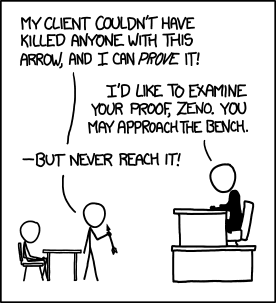
\includegraphics[width=0.2\textwidth]{background/pix/xkcdzeno.png}
    \\
    \protect\label{fig:xkcdzeno}\protect\href{https://xkcd.com/1153/}{由 \protect\url{xkcd.com} 提供}
    \protect\end{center}

}}\index{Zeno's Paradox}\index{paradox!Zeno's}（约公元前450年）。
他设想出一只慢吞吞的乌龟向敏捷的阿基里斯挑战赛跑，
只要求一点领先优势。
阿基里斯笑了，但乌龟说，等阿基里斯
跑到起跑领先位置~$x_0$ 时，乌龟早就已经前进到了某个点~$x_1$。
等跑到~$x_1$，阿基里斯会发现乌龟又跑到了~$x_2$。
对于任意的 $x_i$，
阿基里斯都会落在后面，因此乌龟推论道，阿基里斯永远不可能领先。
这个论证的核心在于，虽然\citetext{距离 $x_{i+1}-x_i$ 趋近于零，
  但由于区间 $\open{0}{\infty}$ 左端的开放性，
  永远有路要走}{%
  一个与此类似、利用了数的无界性的现代悖论是 Thomson 灯悖论：~a
  一个人打开房间的灯，一分钟后关掉，
  半分钟后再打开，四分之一分钟后再关掉，如此等等。
  两分钟后，灯是亮着还是关着？
  这个悖论由 J F~Thomson（汤姆森）于1954年提出，旨在
  分析超任务的可能性，即完成无限多个任务。J F~Thomson 的结论是这会产生矛盾：
  “灯不可能亮着，因为我从来没有只开灯而不立刻关掉它。
  灯也不可能关着，因为我一开始确实开了灯，并且
  此后我也从来没有只关灯而不立刻打开它。
  但灯要么亮着，要么关着”\autocite{Thomson}。
  另见关于
  Littlewood 悖论的讨论 \autocite{wiki:LittlewoodParadox}。}。


\begin{fig}{埃利亚的芝诺向青年们展示通往真理与谬误之门，% (\textit{Veritas et Falsitas})
  通过先走到门的一半距离，再走剩下的一半，如此等等。
  % Bartolomeo Carducci (1560-1608) or Pellegrino Tibaldi (1527–1596).}
  （作者为 B~Carducci（卡杜奇）（1560--1608）或 P~Tibaldi（蒂巴尔迪）（1527--1596）。）}
  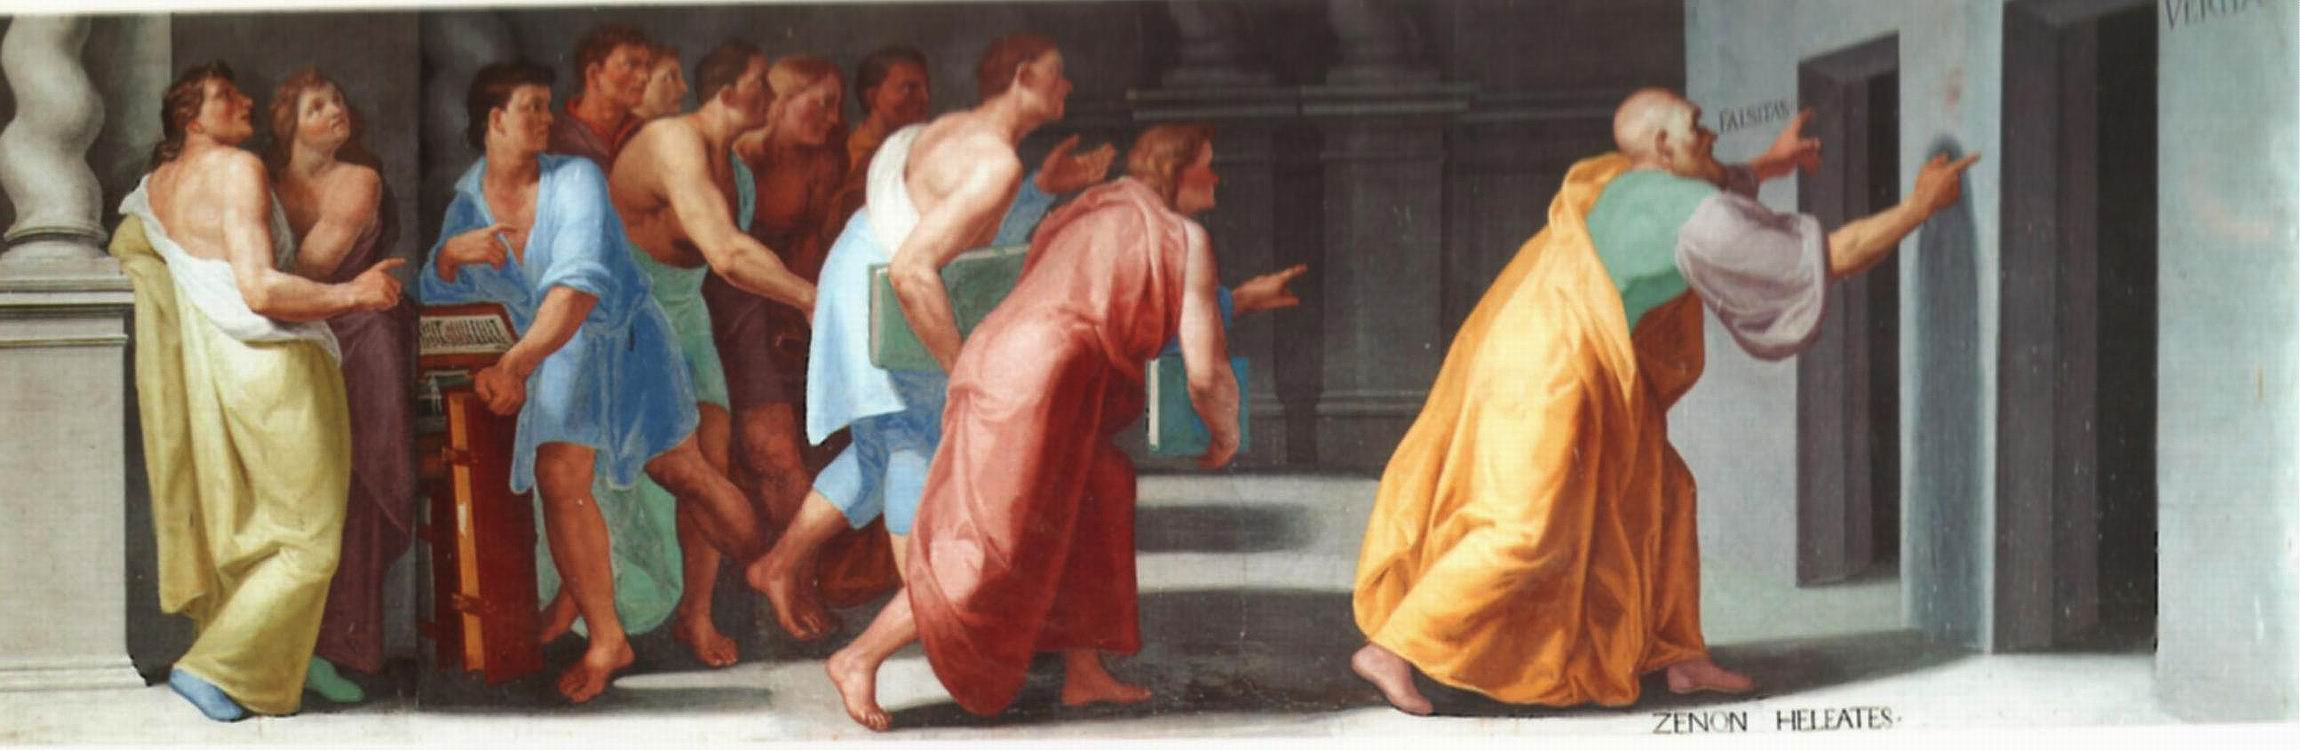
\includegraphics[width=0.8\textwidth]{background/pix/zeno.jpg}
  % PD: https://commons.wikimedia.org/wiki/File:Zeno_of_Elea_Tibaldi_or_Carducci_Escorial.jpg
\end{fig}


\noindent
这个悖论与本小节内容之间的联系，
以及本书后面给出的许多论证，
在于我们常常利用无界性。
不同之处在于，这里以及后面我们关注的是
自然数的无界性，即
$\N$ 在无穷远处的开放性。

\begin{exercises}
\recommended


\begin{exercise}
验证 \zcref{ex:MultiplesOfThreeCountable}，即由 $\map{g}{\N}{\set{3k\suchthat k\in\N}}$ $n\mapsto 3n$ 给出的函数
既是一一的又是满射的。
\begin{answer} \verified
为证明该映射是一一的，我们将证明 $g(n)=g(\hat{n})$ 仅当 $n=\hat{n}$ 时成立。
因此设 $g(n)=g(\hat{n})$，得 $3n=3\hat{n}$。
两边除以三得 $n=\hat{n}$。

为证明该映射是满射的，我们将证明陪域中每个成员
$y\in\set{3k\suchthat k\in\N}$ 都是定义域中某个成员的像。
因为 $y$ 是三的倍数，$y/3$ 是一个自然数。
由于 $y=g(y/3)$，可知 $y$ 确实是定义域中某个成员的像。
\end{answer}
\end{exercise}

\begin{exercise}
一位朋友说：“完全平方数和完全立方数的元素个数相同，因为这两个集合都
既是一一的又是满射的。”
这说法不对；纠正他们。
\begin{answer}  \verified
这是一个类型错误。
一一的或满射的不是集合本身；而是集合之间的对应关系 $f$。
对于 $D=\set{n^2\suchthat n\in\N}$ 和
$C=\set{n^3\suchthat n\in\N}$，自然的这种对应关系
$\map{f}{D}{C}$ 是 $f(n)= n^{3/2}$。
\end{answer}
\end{exercise}

\begin{exercise}
令 $\map{f,g}{\Z}{\Z}$ $f(x) = 2x$ 且 $g(x) = 2x-1$。
对以下各项给出证明或反例。
\begin{exparts*}
\item $f$ 是一一的吗？是满射的吗？
\item $g$ 是一一的吗？是满射的吗？
\item $f$ 和 $g$ 互为逆函数吗？
\end{exparts*}
\begin{answer}  \verified
\begin{exparts}
\item  由 $f(x) = 2x$ 给出的函数 $\map{f}{\Z}{\Z}$ 是一一的，但不是满射的。
  验证它为一一是常规做法：假设对于 $x,\hat{x}\in\Z$ 有 $f(x)=f(\hat{x})$，
  于是 $2x=2\hat{x}$，然后约去 $2$ 得到 $x=\hat{x}$。
  要证明它不是满射的，只需指出一个陪域元素 $y\in\Z$，
  它不是任何定义域元素的像。
  一个这样的例子是 $y=1$，因为每个定义域元素的像都是偶数。
\item  由 $g(x) = 2x-1$ 给出的函数 $\map{g}{\Z}{\Z}$ 也是一一的，但不是满射的。
  一一性的论证与上一项类似：假设对于 $x,\hat{x}\in\Z$ 有 $g(x)=g(\hat{x})$，
  于是 $2x-1=2\hat{x}-1$。
  两边加 $1$ 然后约去 $2$，得到 $x=\hat{x}$。
  这个函数不是满射的，因为陪域元素 $y=2$ 不是任何定义域元素的像，
  因为 $y=2$ 是偶数，而对任何输入整数 $x$，数 $2x-1$ 都是奇数。
\item  它们不互为逆函数。
  例如，$\composed{f}{g}\,(1)=f(g(1))=f(1)=2$。
\end{exparts}
\end{answer}
\end{exercise}

\recommended


\begin{exercise}  % credit: http://www.oxfordmathcenter.com/drupal7/node/205
判断以下每个函数是一一的、满射的、两者都是还是两者都不是。
不能只回答“是”或“否”，必须说明理由。
\begin{exparts}
\item 由 $f(n)=n+1$ 给出的函数 $\map{f}{\N}{\N}$
\item 由 $f(n)=n+1$ 给出的函数 $\map{f}{\Z}{\Z}$
\item 由 $f(n)=2n$ 给出的函数 $\map{f}{\N}{\N}$
\item 由 $f(n)=2n$ 给出的函数 $\map{f}{\Z}{\Z}$
% \item $\map{f}{\N}{\N}$ given by $f(n)=2n+1$
% \item $\map{f}{\Z}{\Z}$ given by $f(n)=2n+1$
% \item $\map{f}{\Z}{\N}$ given by $f(n)=|n|/2$
\item 由 $f(n)=\sizeof{n}$ 给出的函数 $\map{f}{\Z}{\N}$
\end{exparts}
\begin{answer} \verified
\begin{exparts}
\item 由 $f(n)=n+1$ 给出的函数 $\map{f}{\N}{\N}$ 是一一的但不是满射的。
  验证一一性：假定 $n_0,n_1\in\N$ 满足 $f(n_0)=f(n_1)$，
  从而 $n_0+1=n_1+1$，然后两边减去 $1$ 得到 $n_0=n_1$。
  它不是满射的，因为陪域元素 $0\in\N$ 不是任何定义域元素的像。
\item 由 $f(n)=n+1$ 给出的映射 $\map{f}{\Z}{\Z}$ 是一个对应——它既是一一的又是满射的。
  一一性验证：假定 $f(n_0)=f(n_1)$，
  从而 $n_0+1=n_1+1$，减去 $1$ 得到 $n_0=n_1$。
  满射性验证：固定某个陪域元素 $y\in\Z$，
  注意定义域元素 $x=y-1$ 满足 $f(x)=y$。
\item 由 $f(n)=2n$ 给出的函数 $\map{f}{\N}{\N}$ 是一一的但不是满射的。
  对于一一性，假定 $n_0,n_1\in\N$ 满足 $f(n_0)=f(n_1)$。
  于是 $2n_0=2n_1$，消去 $2$ 得到 $n_0=n_1$。
  它不是满射的，因为陪域元素 $y=1$ 不是任何定义域元素的像，因为所有的像都是偶数。
\item 由 $f(n)=2n$ 给出的函数 $\map{f}{\Z}{\Z}$ 是一一的但不是满射的。
  一一性验证与上一项类似：假定对于某些 $n_0,n_1\in\Z$ 有 $f(n_0)=f(n_1)$，
  则 $2n_0=2n_1$，消去 $2$ 得到 $n_0=n_1$。
  同样如上一项，此映射不是满射的，
  因为陪域元素 $y=1$ 不在函数的值域内，因为所有值域元素都是偶数。
\item 由 $f(n)=\sizeof{n}$ 给出的函数 $\map{f}{\Z}{\N}$ 不是一一的，但是满射的。
  它不是一一的，因为两个定义域元素 $n_0=-1$ 和 $n_1=1$ 映射到相同的输出：$f(n_0)=2=f(n_1)$。
  为证明 $f$ 是满射映射，考虑陪域元素 $y\in\N$，
  并注意到若取定义域元素 $x\in\Z$ 使得 $x=y$，那么有 $f(x)=y$。
\end{exparts}
\end{answer}
\end{exercise}

\begin{exercise}
判断以下每一个是否是对应（你必须加以验证）：
\begin{exparts*}
\item 由 $f(q)=q+3$ 给出的 $\map{f}{\Q}{\Q}$
\item 由 $f(n)=n+3$ 给出的 $\map{f}{\Z}{\Q}$
\item 由 $f(a/b)=\sizeof{a\cdot b}$ 给出的 $\map{f}{\Q}{\N}$
% \hint~this could be though of as a trick question.
\end{exparts*}
\begin{answer} \verified
\begin{exparts}
\item 这个函数是一个对应。
  要验证它是一一的，假定 $f(q_0)=f(q_1)$，
  其中 $q_0,q_1\in\Q$，
  从而 $q_0+3=q_1+3$，两边减去 $3$ 得到 $q_0=q_1$。
  对于满射性，考虑陪域元素 $y\in\Q$，
  注意由 $q=y-3$ 给出的定义域元素 $q\in\Q$ 满足 $f(q)=y$。
\item 这个函数不是一个对应。
  它不是满射的，因为陪域元素 $1/2 \in\Q$ 不是任何一个定义域元素 $z\in\Z$ 的像，
  因为每个这样的像 $f(z)=z+3$ 都是整数。
  （这个函数是一一的：假定 $f(z_0)=f(z_1)$，
  从而 $z_0+3=z_1+3$，两边减去 $3$ 得到 $z_0=z_1$。
  但由于它不是满射的，所以它不是对应。）
\item 这不是一个对应。
  它甚至不是一个函数，因为它不是良定义的——
  两个有理数 $q_0=1/2$ 和 $q_1=2/4$ 相等，即 $q_0=q_1$，
  但它们对应的 $\sizeof{a\cdot b}$ 值不同，
  因为 $\sizeof{1\cdot 2}=2$ 而 $\sizeof{2\cdot 4}=8$。
\end{exparts}
\end{answer}
\end{exercise}

\begin{exercise}
判断以下每个集合是有限的还是无限的，并论证你的答案。
\begin{exparts*}
\item $\set{1,2,3}$
\item $\set{0,1,4,9,16,\ldots}$
\item 素数集合
\item 方程 $x^5-5x^4+3x^2+7$ 的实根集合
\end{exparts*}
\begin{answer}  \verified
\begin{exparts}
\item 这个集合是有限的。
  它与 $I=\set{0,1,2}$ 有相同的势，
  由 $f(x)=x+1$ 给出的函数 $\map{f}{I}{\set{1,2,3}}$ 见证，通过观察可知该映射是一一的且满射的。
\item 由完全平方数组成的集合 $S=\set{0,1,4,9,16,\ldots}$ 是无限的。
  不存在 $I=\set{0,1,\ldots\, n-1}$ 和 $S$ 之间的对应，因为不存在满射函数——对于
  任何函数 $\map{f}{I}{S}$，集合 $\set{f(0),f(1),\ldots\, f(n-1)}$ 不可能等于 $S$，
  因为前者有一个最大元素，而 $S$ 没有最大元素。
\item 素数集合是无限的。
  上一项的论证同样适用。
\item 根据算术基本定理，一个五次多项式至多有五个实数根。
  因此这个集合的势至多为五，所以是有限的。
\end{exparts}
\end{answer}
\end{exercise}

% \begin{exercise}
% Prove that
% the set $\N-\set{0}=\set{1,2,\ldots}$ is countable, using as a correspondence
% the function $\map{f}{\N}{\N-\set{0}}$ given by
% $f(n)=n+1$.
% \begin{answer}
% The function $f$ is one-to-one because if $f(n_0)=f(n_1)$ then
% $n_0+1=n_1+1$ and so~$n_0=n_1$.
% It is onto because if $y$ is an element of the
% codomain~$\N-\set{0}=\set{1,2,\ldots}$ then $y$ is the image of $y-1$,
% that is, $y=f(y-1)$,
% and clearly $y-1$ is an element of the domain~$\N$.
% \end{answer}
% \end{exercise}

\begin{exercise}
通过构造从一个集合到另一个集合的一一的且满射的函数，来证明下列每对集合具有相同的势。
你必须验证该函数是一个对应。
\begin{exparts*}
\item $\set{0,1,2}$, $\set{3,4,5}$
\item $\Z$, $\set{i^3\suchthat i\in\Z}$
\end{exparts*}
\begin{answer} \verified
\begin{exparts}
\item 映射 $\map{f}{\set{0,1,2}}{\set{3,4,5}}$ 由 $f(0)=3$, $f(1)=4$, $f(2)=5$ 给出，即 $f(x)=x+3$，是一个对应。
  经检查，陪域中的每个元素都与定义域中唯一的一个元素相关联。
\item 函数 $f(x)=x^3$ 是这些集合之间的一个对应。
  对于每个完全立方数，都有且仅有一个与之关联的整数立方根。
\end{exparts}
\end{answer}
\end{exercise}

\recommended


\begin{exercise}
通过构造一个对应（你必须验证该函数是一个对应），来证明下列每对集合具有相同的势：
\begin{exparts*}
\item $\set{0,1,3,7}$ 和 $\set{\pi,\pi+1,\pi+2,\pi+3}$
\item 偶自然数与完全平方数
\item 实数区间 $\open{1}{4}$ 与 $\open{-1}{1}$。
\end{exparts*}
\begin{answer} \verified
\begin{exparts}
\item 函数 $f$ 由 $0\mapsto\pi$, $1\mapsto\pi+1$, $3\mapsto\pi+2$, $7\mapsto\pi+3$ 给出，经检查可知它既是一一的又是满射的。
\item 令 $E=\set{2n\suchthat n\in\N}$ 且 $S=\set{n^2\suchthat n\in\N}$。
  考虑由 $f(x)=(x/2)^2$ 给出的映射 $\map{f}{E}{S}$。
  为证明 $f$ 是一一的，假设 $f(x_0)=f(x_1)$。
  那么 $(x_0/2)^2=(x_1/2)^2$，并且由于这些是自然数，它们的平方根相等，即 $x_0/2=x_1/2$。
  因此 $x_0=x_1$，该映射是一一的。

  为证明满射性，任取 $y\in S$。
  因为 $y$ 是一个完全平方数，所以存在自然数 $n\in\N$ 使得 $y=n^2$。
  令 $x=2n$。
  显然 $x$ 是偶数，且 $f(x)=y$。
\item 第二个区间的宽度是第一个的 $2/3$，因此考虑函数 $f(x)=(2/3)\cdot x-(5/3)$。
  它是一一的，因为 $f(x_0)=f(x_1)$ 意味着 $(2/3)\cdot x_0-(5/3)=(2/3)\cdot x_1-(5/3)$，通过简单的代数运算可得 $x_0=x_1$。
  要证明 $f$ 是满射的，固定 $y\in\open{-1}{1}$。
  令 $x=(y+(5/3))\,/\,(2/3)$（这来自于从方程 $y=(2/3)x-(5/3)$ 解出 $x$）。
  当 $y$ 是陪域 $\open{-1}{1}$ 中的一个元素时，这个 $x$ 便是定义域 $\open{1}{4}$ 中的一个元素，并且进一步的代数运算表明 $f(x)=y$。
\end{exparts}
\end{answer}
\end{exercise}

\recommended


\begin{exercise}
验证函数 $f(x)=1/x$ 是 $\R$ 的子集 $\open{0}{1}$ 与~$\open{1}{\infty}$ 之间的一个对应。
\begin{answer} \verified
题目的表述在哪个集合是定义域、哪个是陪域方面有些含糊。
我们将证明由 $f(x)=1/x$ 给出的 $\map{f}{\open{0}{1}}{\open{1}{\infty}}$ 既是一一的又是满射的。

为证一一性，假设 $f(x_0)=f(x_1)$，其中 $x_0,x_1\in\open{0}{1}$。
那么 $1/x_0=1/x_1$，交叉相乘可得 $x_1=x_0$。
为证满射性，设 $y\in\open{1}{\infty}$，并注意到若取 $x=1/y$，则 $f(x)=y$ 且也有 $x\in\open{0}{1}$。
\end{answer}
\end{exercise}

\begin{exercise}
给出集合 $\set{1,2,3,4,\ldots}$ 与
$\set{7,10,13,16\ldots}$ 之间的对应的公式。
\begin{answer}\verified
将这两个集合记为 $D=\set{1,2,3,4,\ldots}$ 和
$C=\set{7,10,13,16\ldots}$。
我们将证明由公式 $f(x)=3(x-1)+7$ 所描述的映射 $\map{f}{D}{C}$ 是这两个集合之间的一个对应。
该函数是一一的，因为由 $f(x_0)=f(x_1)$ 可推出
$3(x_0-1)+7=3(x_1-1)+7$，然后减去 $7$，除以 $3$，再加 $1$ 便得到 $x_0=x_1$。
它是满射的，因为如果 $y$ 是陪域 $C$ 中的一个元素，则对于某个 $n\in\N^+$，它具有形式 $y=3n+4$。
这个等式可以写成 $y=3(n-1)+7$。
经代数运算可得，对于 $n\in\N^+$，有 $(y-7)/3=n-1$，并且 $n=((y-7)/3)+1$ 是属于 $\N^+=D$ 的一个元素，且满足 $f(n)=y$。
\end{answer}
\end{exercise}

\recommended


\begin{exercise}
考虑字符集 $C=\set{\str{0},\ \str{1}, \ldots\, \str{9}}$
与整数集 $A=\set{48, 49, \ldots\, 57}$。
\begin{exparts}
\item 构造一个对应 $\map{f}{C}{A}$。
\item 验证其逆 $\map{f^{-1}}{A}{C}$ 也是一个对应。
\end{exparts}
\begin{answer}\verified
\begin{exparts}
\item 最直观的映射如下。
\begin{center}
\begin{tabular}{r|*{10}{c}}
  $x$    &\str{0} &\str{1} &\str{2} &\str{3} &\str{4} &\str{5}
           &\str{6} &\str{7} &\str{8} &\str{9}     \\  \cline{1-11}
  $f(x)$ &$48$ &$49$ &$50$ &$51$ &$52$ &$53$ &$54$ &$55$ &$56$ &$57$
   \rule{0em}{2.2ex}  % scootch more room over the f
\end{tabular}
\end{center}
通过观察可知它是一一的，这意味着观察这个关联可以看出，绝不会有两个不同的定义域元素映射到同一个陪域元素。
类似地，通过观察可知它也是满射的。
\item 逆映射关联了前一项表格中相同的元素对，但定义域和陪域互换了位置，因此这里 $A$ 是定义域，$C$ 是陪域。
\begin{center}
\begin{tabular}{r|*{10}{c}}
  $y$    &$48$ &$49$ &$50$ &$51$ &$52$ &$53$ &$54$ &$55$ &$56$ &$57$
    \\  \cline{1-11}
  $x$    &\str{0} &\str{1} &\str{2} &\str{3} &\str{4} &\str{5}
           &\str{6} &\str{7} &\str{8} &\str{9}
\end{tabular}
\end{center}
如前一项，通过观察可知这个映射既是一一的又是满射的。
\end{exparts}
\end{answer}
\end{exercise}

\recommended


\begin{exercise}
证明下列每对集合具有相同的势。
你必须给出一个合适的函数，并验证它既是一一的又是满射的。
\begin{exparts*}
\item $\N$ 与偶数集
\item $\N$ 与奇数集
\item 偶数集与奇数集
\end{exparts*}
\begin{answer}\verified
对于每对集合，我们可以定义一个以第一个集合为定义域的函数，或者定义一个以第二个集合为定义域的函数。
我们选择较为方便的一种。
\begin{exparts}
\item 将偶数表示为 $E=\set{2n\suchthat n\in\N}$。
考虑函数 $\map{f}{\N}{E}$，
定义为 $f(m)=2m$。
为了验证 $f$ 是一一的，假设两个输入得到相同的输出 $f(m)=f(\hat{m})$，得到 $2m=2\hat{m}$，然后除以~$2$ 得到这两个输入相同，即 $m=\hat{m}$。

为了验证 $f$ 是满射的，考虑陪域中的一个元素 $y\in E$，
因此对于某个 $n\in\N$，有 $y=2n$。
那么，$n=y/2$ 满足 $f(n)=y$。
注意 $n$ 是定义域~$\N$ 中的一个元素，因为作为陪域中的元素，$y$ 是偶数，所以除以二会得到一个自然数。
\item 将奇数表示为 $M=\set{2n+1\suchthat n\in\N}$。
考虑 $\map{g}{\N}{M}$，定义为 $n\mapsto 2n+1$。
为了验证 $g$ 是一一的，假设 $g(m_0)=g(m_1)$，
因此 $2m_0+1=2m_1+1$，减去~$1$，然后除以~$2$，得到 $m_0=m_1$。

为了验证 $g$ 是满射的，从陪域中的一个元素 $y\in M$ 出发。
那么它具有形式 $y=2k+1$，其中 $k$ 是某个自然数。
这意味着存在一个自然数~$k$ 在~$g$ 下映射到~$y$，即 $k=(y-1)/2$。
\item 一种答案是引用前面的两个小题，并利用对应的逆也是对应这一结论，得到复合 $\composed{g}{f^{-1}}$ 是从偶数到奇数的一个对应。

另一种直接的回答是考虑映射~$\map{p}{E}{M}$，
定义为 $p(n)=n+1$。
如同前两项那样验证 $p$ 既是一一的又是满射的。
\end{exparts}
\end{answer}
\end{exercise}

\recommended


\begin{exercise}
虽然有时存在自然的对应，但对应不必唯一。
给出从 $\open{0}{1}$ 到 $\open{0}{2}$ 的自然对应，然后给出一个不同的对应，再给出另一个不同的对应。
\begin{answer}\verified
自然的对应 $\map{f_0}{\open{0}{1}}{\open{0}{2}}$ 是 $f_0(x)=2x$。
对于另外两个对应，有许多选择，但另外两个对应 $\map{f_0,f_1,f_2}{\open{0}{1}}{\open{0}{2}}$ 是
$f_1(x)=2-2x$ 和~$f_2(x)=2x^2$。
\figureref{fig:ThreeCorrespondencesFromUnitInt} 展示了这三个函数的图像。
\begin{figure}
  \centering
  \vcenteredhbox{\includegraphics{\asydir maps/maps04.pdf}}
  \qquad
  \vcenteredhbox{\includegraphics{\asydir maps/maps05.pdf}}
  \qquad
  \vcenteredhbox{\includegraphics{\asydir maps/maps06.pdf}}
  \caption{对应 $\map{f_0,f_1,f_2}{\open{0}{1}}{\open{0}{2}}$
由 $f_0(x)=2x$、$f_1(x)=2-2x$ 和~$f_2(x)=2x^2$ 给出。}
  \label{fig:ThreeCorrespondencesFromUnitInt}
\end{figure}
它们是不同的函数，因为它们在输入~$x=1/3$ 处返回不同的值。

每个函数既是一一的又是满射的，因为图像显示对于 $y\in\open{0}{2}$ 的每条水平线与其图像恰好相交于一点。

为了代数地验证它们是对应，我们可以以~$f_1$ 为例。
它是一一的，因为如果 $f(x_0)=f(x_1)$ 那么
$2-2x_0=2-2x_1$，然后减去~$2$ 并除以~$-2$ 得到 $x_0=x_1$。
它是满射的，因为如果 $y\in\open{0}{2}$，那么数~$x=(y-2)/(-2)$ 是
$\open{0}{1}$ 中的一个元素，且满足 $f(x)=2-2\cdot((y-2)/-2)=y$。
\end{answer}
\end{exercise}

\begin{exercise}
\zcref{ex:PerfectSquaresCountable} 给出了一种自然数与完全平方数之间的对应。
请给出另一种。
\begin{answer}\verified
函数
\begin{equation*}
  \hat{f}(n)=
  \begin{cases}
    1    &\case{if $n=0$}  \\
    0    &\case{if $n=1$}  \\
    n^2  &\case{if $n>1$}
  \end{cases}
\end{equation*}
与 \zcref{ex:PerfectSquaresCountable} 中的函数~$f$ 不同，
因为它们在输入~$0$ 时给出不同的输出。
$\hat{f}$ 是满射的这一点很清楚，
因为每个完全平方数都是某个输入对应的输出。
$\hat{f}$ 是一个一一函数这一点也很清楚，
尽管写下来证明会稍显繁琐。
假设 $\hat{f}(x_0)=\hat{f}(x_1)$，然后分四种情况：$x_0$ 和~$x_1$ 都属于集合~$\set{0,1}$，
只有第一个属于，只有第二个属于，或者两者都不属于。
所有四种情况都很容易处理。
\end{answer}
\end{exercise}

\begin{exercise}
取定 $c\in\R$ 使得 $c>1$。
证明由 $x\mapsto c^x$ 给出的 $\map{f}{\R}{\open{0}{\infty}}$ 是一个对应。
\begin{answer}  \verified
为验证~$f$ 是一一的，假设 $f(x_0)=f(x_1)$，
于是有 $c^{x_0}=c^{x_1}$。
两边取以~$c$ 为底的对数，得 $x_0=x_1$。

对于满射，考虑陪域中的元素 $y\in\open{0}{\infty}$。
数 $x=\log_{c}(y)$ 有定义且是~$f$ 的定义域~$\R$ 中的一个元素。
显然，$f(x)=f(\log_c(y))=c^{\log_c(y)}=y$。
\end{answer}
\end{exercise}

\begin{exercise}
证明2的幂的集合 $\set{2^k\suchthat k\in\N}$ 和3的幂的集合 $\set{3^k\suchthat k\in\N}$ 同势。
请加以推广。
\begin{answer}\verified
两个集合
$P_2=\set{2^k\suchthat k\in\N}=\set{1,2,4,8,\ldots}$
和 $P_3=\set{3^k\suchthat k\in\N}=\set{1,3,9,\ldots}$ 都是~$\N$ 的子集。
自然的对应 $\map{g}{P_2}{P_3}$ 是将具有相同指数的元素关联起来，即 $g(2^k)=3^k$。
这个函数是一一的，因为如果~$g(2^{k_0})=g(2^{k_1})$ 那么
$3^{k_0}=3^{k_1}$，两边取以~$3$ 为底的对数表明输入是相同的，即~$k_0=k_1$。
这个函数是满射的，因为如果 $y\in P_3$，则其形式为 $y=3^k$，
并且它是 $P_2$ 中~$2^k$ 的像。

明显的推广是：如果两个自然数 $a,b\in\N$ 都大于~$1$，那么 $P_a=\set{a^k\suchthat k\in\N}$ 和
$P_b=\set{b^k\suchthat k\in\N}$ 是同势的自然数集合。
论证过程同前一段。
\end{answer}
\end{exercise}

\begin{exercise}
对于以下各项，给出从 $\N$ 到其自身的函数。
你必须论证你的结论。
\begin{exparts*}
\item 给出两个一一但不满射的函数的例子。
\item 给出两个满射但不是一一的函数的例子。
\item 给出两个既不一一也不满射的例子。
\item 给出两个既一一又满射的例子。
\end{exparts*}
\begin{answer}\verified
当然，对于每一项都有许多可能的答案。
\begin{exparts}
\item
一个是 $\map{f_0}{\N}{\N}$，定义为 $f_0(n)=n+1$。
它是一一的，因为如果 $f_0(n)=f_0(\hat{n})$，那么 $n+1=\hat{n}+1$，
从而 $n=\hat{n}$。
它不是满射的，因为没有 $n\in\N$ 映射到~$0$。

第二个是 $\map{f_1}{\N}{\N}$，定义为 $f_1(n)=n^2$。
它是一一的，因为如果 $f_1(n)=f_1(\hat{n})$，那么 $n^2=\hat{n}^2$，
且由于自然数皆非负，所以 $n=\hat{n}$。
这个函数不是满射的，因为没有自然数映射到~$2$。
\item
函数
\begin{equation*}
  f_0(x)=
  \begin{cases}
    x/2      &\case{if $x$ is even}  \\
    (x-1)/2  &\case{if $x$ is odd}
  \end{cases}
  \qquad
  \begin{array}{r|*{7}{c}}
    x      &0 &1 &2 &3 &4 &5 &\ldots  \\ \cline{2-8}
    f_0(x) &0 &0 &1 &1 &2 &2 &\ldots
  \end{array}
\end{equation*}
是满射的，因为每个 $y\in\N$ 都是 $x=2y$ 的像。
它不是一一的，因为 $f_0(1)=f_0(0)$。

第二个是 $f_1(x)=\floor{\sqrt{x}}$
（回顾向下取整运算 $\floor{n}$ 给出小于或等于~$n$ 的最大整数）。
\begin{equation*}
  \begin{array}{r|*{12}{c}}
    x      &0 &1 &2 &3 &4 &5 &6 &7 &8 &9 &10 &\ldots  \\ \cline{2-13}
    f_1(x) &0 &1 &1 &1 &2 &2 &2 &2 &2 &3 &3  &\ldots
  \end{array}
\end{equation*}
它是满射的，因为每个 $y\in\N$ 都是 $x=y^2$ 的像。
它不是一一的，因为 $f_1(1)=f_1(2)$。
\item
一个这样的映射是 $f_0(x)=0$。
它不是一一的，因为 $f_0(0)=f_0(1)$。
它不是满射的，因为没有自然数映射到~$1$。

另一个非常数的此类函数是前一项中第二个函数的平方，
$f_1(x)=(\floor{\sqrt{x}})^2$。
\begin{equation*}
  \begin{array}{r|*{12}{c}}
    x      &0 &1 &2 &3 &4 &5 &6 &7 &8 &9 &10 &\ldots  \\ \cline{2-13}
    f_1(x) &0 &1 &1 &1 &4 &4 &4 &4 &4 &9 &9  &\ldots
  \end{array}
\end{equation*}
它不是一一的，因为 $f_1(1)=f_1(2)$。
由于 $2$ 不是平方数，它不是满射的，没有数映射到~$2$。
\item
最直观的既一一又满射的函数是恒等函数 $f_0(x)=x$。
它是一一的，因为如果 $f_0(n)=f_0(\hat{n})$，那么~$n=\hat{n}$，
直接根据~$f_0$ 的定义可得。
它是满射的，因为任何陪域元素 $y\in\N$ 都是其自身在~$f_0$ 下的像，
即 $f_0(y)=y$。

另一个对应交换偶数和奇数。
\begin{equation*}
  f_1(x)=
  \begin{cases}
    x+1  &\case{if $x$ is even}  \\
    x-1  &\case{if $x$ is odd}
  \end{cases}
  \qquad
  \begin{array}{r|*{7}{c}}
    x      &0 &1 &2 &3 &4 &5 &\ldots  \\ \cline{2-8}
    f_1(x) &1 &0 &3 &2 &5 &4 &\ldots
  \end{array}
\end{equation*}
首先注意 $\map{f_1}{\N}{\N}$；即，如果 $x\in\N$，那么 $f_1(x)\in\N$。
为验证~$f_1$ 是一一的，假设 $f_1(n)=f_1(\hat{n})$。
有两种情况。
如果 $n$ 是奇数，则 $f_1(n)=n-1$ 是偶数，因此 $f_1(\hat{n})$ 也是偶数，
这意味着 $\hat{n}$ 是奇数，从而 $n-1=\hat{n}-1$，得 $n=\hat{n}$。
偶数情况类似。
为验证~$f_1$ 是满射的，考虑陪域点 $y\in\N$。
这里也有两种情况，我们只做奇数情况，假设 $y$ 是奇数。
那么 $y=f_1(x)$ 其中 $x=y-1$，且 $x$ 是定义域~$\N$ 中的一个元素，
因为如果 $y$ 是奇数，则 $y-1\geq 0$。
\end{exparts}
\end{answer}
\end{exercise}

\begin{exercise}
通过构造一个对应，证明实数区间
$\open{3}{5}$ 和~$\open{-1}{10}$ 同势。
然后再构造另一个。
\begin{answer} \verified
令 $D=\open{3}{5}$ 和~$C=\open{-1}{10}$。

一种对应是 $f_0(x)=(11/2)(x-3)-1$。
$\map{f_0}{D}{C}$ 并不显然，因此我们先验证这一点：如果
$3< x<5$，先减去~$3$，
再乘以 $11/2$，然后对所有项减去~$1$，
得到 $-1< f_0(x)< 10$。
接着，我们证明这个映射是满射的。
如果 $y\in C$，那么 $y=f_0(x)$，其中 $x=(2/11)(y+1)+3$。
要验证这个输入~$x$ 是定义域~$D$ 的元素，
从 $-1<y<10$ 出发，对所有项加~$1$，
乘以 $2/11$，再加~$3$，最终得到 $3<x<5$。
最后，我们证明映射~$f_0$ 是一一的。
如果 $f_0(x)=f_0(\hat{x})$ 那么
$(11/2)(x-3)-1=(11/2)(\hat{x}-3)-1$，
两边加~$1$，乘以 $2/11$，
最后加~$3$，得
$x=\hat{x}$。

另一种对应是 $f_1(x)=(11/4)(x-3)^2-1$。
与~$f_0$ 类似，我们首先验证 $\map{f_1}{D}{C}$：如果
$3< x<5$，先减去~$3$，平方，
乘以 $11/4$，再对所有项减去~$1$，
得到 $-1< f_1(x)< 10$。
为证明~$f_1$ 是满射的，假设 $y\in C$。
那么 $y=f_1(x)$，其中 $x=\sqrt{(4/11)(y+1)}+3$。
要验证 $x\in D$，从 $-1<y<10$ 出发，对所有项加~$1$，
乘以 $4/11$，
平方（因为所有数均非负，这不会改变不等号的方向），再加~$3$，最终得到 $3<x<5$。
为证明此映射是一一的，假设 $f_1(x)=f_1(\hat{x})$ 从而有
$(11/4)(x-3)^2-1=(11/4)(\hat{x}-3)^2-1$。
等式两边加~$1$，乘以 $4/11$，开平方根
（因为所有 $x$ 均大于零，该操作是确定的），
再加~$3$，得
$x=\hat{x}$。

\figureref{fig:TwoCorrespondences}
表明这两个函数不相同。
它还提供了另一种论证方式证明它们都是对应：
对于每一个函数，在 $y\in\open{-1}{10}$ 处的每一条水平线都会与函数图像相交于恰好一个点。
\begin{figure}
  \centering
  
\includegraphics{\asydir correspondences/correspondences001.pdf}%
  \hspace{2em plus 1fil}
  
\includegraphics{\asydir correspondences/correspondences002}%
  \caption{$\open{3}{5}$ 与 $\open{-1}{11}$ 之间的两个对应。}
  \label{fig:TwoCorrespondences}
\end{figure}
\end{answer}
\end{exercise}

\begin{exercise}
证明以下各组集合同势。
\begin{exparts*}
\item $\set{4k\suchthat k\in\N}$, $\set{5k\suchthat k\in\N}$
\item $\set{0,1,\ldots\, 99}$, $\set{m\in\N\suchthat m^2<10\,000}$
\item $\set{0,1,3,6,10,15,\ldots}$, $\N$
\end{exparts*}
\begin{answer}\verified
在每种情况下，我们都构造一个从一个集合到另一个集合的函数，并验证它既是一一的又是满射的。
对于第三小题，请注意：一个集合在问题中先出现，并不意味着它必须作为对应中的定义域。
\begin{exparts}
\item
令 $S_4=\set{4k\suchthat k\in\N}$ 和 $S_5=\set{5k\suchthat k\in\N}$，
令 $\map{f}{S_4}{S_5}$ 为 $f(x)=(5/4)x$。
它是一一的，因为 $f(x_0)=f(x_1)$ 意味着
$(5/4)x_0=(5/4)x_1$，所以 $x_0=x_1$。
它是满射的，因为如果考虑陪域中的元素 $y=5k$（其中 $k\in\N$），显然有 $y=f(4k)$。
\item
这两个集合是同一个集合，即它们包含相同的数。
它们通过恒等函数构成对应。
\item
记
$T=\set{0,1,3,6,\ldots}=\set{n(n+1)/2\suchthat n\in \N}$
（这些数被称为三角数）。
考虑函数 $\map{f}{\N}{T}$，其定义为
$f(n)=n(n+1)/2$。
该映射是一一的，因为连续函数
$\map{\hat{f}}{\R}{\R}$（由 $\hat{f}(x)=x(x+1)/2$ 给出）
是一个根为 $0$ 和~$-1$ 的抛物线，因此在 $x\geq 0$ 的正数部分，
水平线~$y$ 最多与图像相交于一个点。
$\hat{f}$ 是一一的这一事实意味着它的限制~$f$ 也是一一的。
由定义可知函数~$f$ 是满射的，因为 $T$ 被定义为该函数的值域。
\end{exparts}
\end{answer}
\end{exercise}

% \begin{exercise}
% Prove that the set  $\set{10k\suchthat k\in\N}$ of multiples of ten
% is countable.
% \begin{answer}
% Call the set $T=\set{10k\suchthat k\in\N}$.
% The function $\map{f}{\N}{T}$ given by $f(n)=10n$ is a correspondence.
% It is one-to-one because $f(n)=f(\hat{n})$ implies that $10n=10\hat{n}$,
% and so $n=\hat{n}$.
% It is onto because by definition any member of $T$ has the form $10k$
% for some~$k\in\N$, and so is the image under~$f$ of~$k$.
% \end{answer}
% \end{exercise}

\recommended

\begin{exercise}
为下列每一对实数开区间构造一个对应。
\begin{exparts}
\item $\open{0}{1}$, $\open{0}{2}$
\item $\open{0}{1}$, $\open{a}{b}$，其中 $a<b$ 为实数
\item $\open{0}{\infty}$, $\open{a}{\infty}$，其中 $a$ 为实数
\item
下图展示了一个从有限实数区间到无限实数区间的对应 $x\mapsto f(x)$，
$\map{f}{\open{0}{1}}{\open{0}{\infty}}$。
\begin{center}
  
\includegraphics{\asydir correspondences/correspondences000.pdf}
\end{center}
点 $P$ 的坐标为 $(-1,1)$。
请给出 $f$ 的公式。
\end{exparts}
\begin{answer}\verified
\begin{exparts}
\item 一个是 $f(x)=2x$。
  这个映射是一一的，因为如果 $f(x)=f(\hat{x})$，那么 $2x=2\hat{x}$，从而 $x=\hat{x}$。
  它是满射的，因为对于 $0<y<2$，取 $x=y/2$，则有 $f(x)=y$ 且 $0<x<1$。
\item 一个是 $f(x)=(b-a)\cdot x+a$。
  注意，$\map{f}{\open{0}{1}}{\open{a}{b}}$，因为如果 $0<x<1$，那么乘以 $b-a$ 得到 $0<x<(b-a)$（由于 $a<b$，不等号方向不变），再加上 $a$ 即得 $a<x<b$。
  进一步，这个函数是一一的：因为 $b-a\neq 0$，该直线斜率非零，故通过水平线检验（如需代数论证，从 $f(x)=f(\hat{x})$ 出发，减去 $a$ 再除以 $b-a$，可得 $x=\hat{x}$）。
  最后，证明它是满射的。任取 $y\in\open{a}{b}$。注意，取 $x=(y-a)/(b-a)$ 则 $f(x)=y$。
  剩下的就是验证 $x\in\open{0}{1}$：从 $a<y<b$ 出发，减去 $a$ 再除以 $b-a$，得到 $0<(y-a)/(b-a)<1$（如前所述，由于 $b-a>0$，不等号方向不变）。
\item 一个是 $f(x)=x+a$。
  该函数是一一的，因为 $f(x)=f(\hat{x})$ 意味着 $x+a=\hat{x}+a$，从而 $x=\hat{x}$。
  它是满射的，因为如果 $y\in\open{a}{\infty}$，那么令 $x=y-a$（且 $x\in\open{0}{\infty}$），则有 $y=f(x)$。
\item 由相似三角形得到 $x/(x+1)=f(x)/1$。
  \figureref{fig:CorrespondenceZeroInfToZeroOne} 表明这是一个对应，因为对于每个 $y\in\open{0}{1}$，过该高度的水平线与函数图像恰好交于一点。
\begin{figure}
  \centering
  
\includegraphics{\asydir correspondences/correspondences003.pdf}%
  \caption{$\open{0}{\infty}$ 与 $\open{0}{1}$ 之间的一个对应。}
  \label{fig:CorrespondenceZeroInfToZeroOne}
\end{figure}
\end{exparts}
\end{answer}
\end{exercise}

% \begin{exercise}
% Recall that for any set~$S$,
% its power set~$\powerset(S)$\index{power set of a set}\index{set!power set}
% is the collection of subsets of~$S$.
% Show that the power set of the natural numbers~$\powerset(\N)$
% has the same cardinality as the set of functions
% $\map{f}{\N}{\N}$.
% \hint:associate each subset~$A\subseteq\N$ with its characteristic function.
% \begin{answer}

% \end{answer}

% \end{exercise}

\recommended


\begin{exercise}
并非每个包含无理数的集合都是不可数的。
证明集合 $S=\set{\!\sqrt[n]{2}\suchthat \text{$n\in\N$ and $n\geq 2$}}$ 是可数的。
\begin{answer}\verified
考虑由 $f(m)=\!\sqrt[m+2]{2}=2^{1/(m+2)}$ 给出的函数 $\map{f}{\N}{S}$。
它是一一的，因为如果 $f(m)=f(\hat{m})$，则 $2^{1/(m+2)}=2^{1/(\hat{m}+2)}$。
对两边取对数 $\lg(2^{1/(m+2)})=\lg(2^{1/(\hat{m}+2)})$ 得到 $(1/(m+2))\cdot\lg(2)=(1/(\hat{m}+2))\cdot\lg(2)$，于是 $1/(m+2)=1/(\hat{m}+2)$。
因此 $m=\hat{m}$。

该函数是满射的，因为如果 $y\in S$，则存在 $n\in\N$ 且 $n\geq 2$ 使得 $y=2^{1/n}$。
因此，对某个 $x\in\N$，有 $y=2^{1/(x+2)}=f(x)$。
\end{answer}
\end{exercise}

% \begin{exercise}
% Define a correspondence between the set of points on the boundary of the unit
% square and those on the boundary of the unit circle.
% You must show that your function is one-to-one and onto.
% \end{exercise}

% \begin{exercise}
% Prove that a subset of a finite set is finite.
% Is a subset of an infinite set infinite?
% \begin{answer}
% Let $S$ be a finite set, so it is empty or has the same cardinality as
% $\set{0,1,\ldots\, n}$ for some~$n\in\N$.
% If $S$ is empty then its only subset is the empty set, which is finite.
% Otherwise for some $n\in\N$ there is a correspondence
% $\map{f}{S}{\set{0,\ldots\, n}}$.
% \end{answer}
% \end{exercise}

\begin{exercise}
令 $\B$ 为构成比特串的字符集合，$\B=\set{\str{0},\str{1}}$。
\begin{exparts*}
\item 令 $B$ 是以 \str{1} 开头的有限比特串的集合。证明 $B$ 是可数的。
\item 令 $\kleenestar{\B}$ 是有限比特串的集合，没有对首比特的限制。证明它也是可数的。
\hint~利用上一项结果。
\end{exparts*}
\begin{answer}\verified
回想一下，正如每个自然数都有唯一的有限位十进制表示，每个自然数也有唯一的二进制表示。
\begin{exparts}
\item
将每个以 \str{1} 开头的比特串 $\sigma$ 视为某个自然数 $n$ 的二进制表示。
那么，由 $\sigma\mapsto n-1$ 给出的映射 $\map{f}{B}{\N}$ 显然是一个对应。
\item 在每个串 $\tau\in\kleenestar{\B}$ 前添加 \str{1}，即 $\sigma=\str{1}\concat\tau$。
此时便可应用前一项的论证。
\end{exparts}
\end{answer}
\end{exercise}

% \begin{exercise}
% The programming language FORTRAN~77 had a character set consisting of
% upper and lower-case ASCII letters \str{A}--\str{Z} and \str{a}--\str{z},
% numerals \str{0}--\str{9}, and twenty two special characters such as
% \str{=} and \str{/}.
% \begin{exparts}
% \item
% Show that for any $n\in\N$ the number of length~$n$ programs is
% finite.
% \item
% Show that the number of FORTRAN~77 programs is countable.
% \end{exparts}
% \end{exercise}

% \begin{exercise}
% Give a formula for the correspondence whose tabular presentation is shown in
% \zcref{exam:NMatchesTwoN}.
% \end{exercise}

% \begin{exercise}
% Extend the method of \zcref{exam:NMatchesTwoN} to give a correspondence
% between $\N$ and $\set{0,1,2}\times\N$.
% \end{exercise}

\begin{exercise}
利用反正切函数证明集合 $\open{0}{1}$ 和 $\R$ 同势。
\begin{answer}\verified
正切函数是从 $\open{-\pi/2}{\pi/2}$ 到 $\R$ 的对应，所以其逆函数反正切是反方向的对应。
因此，$g(x)=(\arctan(x)+(\pi/2))/\pi$ 给出了一个从 $\R$ 到 $\open{0}{1}$ 的对应。
参见 \figureref{fig:CorrespondenceRAndUnitInterval}，该图表明 $g$ 是一一的且满射的，因为对于陪域 $\open{0}{1}$ 中的每个元素 $y$，过 $y$ 的水平线与函数图像恰好交于一点。
\begin{figure}
  \centering
  
\includegraphics{\asydir correspondences/correspondences004.pdf}
  \caption{$\R$ 与 $\open{0}{1}$ 之间的一个对应。}
  \label{fig:CorrespondenceRAndUnitInterval}
\end{figure}
\end{answer}
\end{exercise}

\begin{exercise} \label{exer:VerifyAsParadox}
\zcref{ex:RealIntervalsCorrespond} 将 Aristotle 悖论重新表述为：对于 $r_0,r_1\in\R^+$，区间 $I_0=\leftclosed{0}{2\pi r_0}$ 与 $I_1=\leftclosed{0}{2\pi r_1}$ 同势。
\begin{exparts}
\item 通过验证由 $g(x)=x\cdot(r_1/r_0)$ 给出的 $\map{g}{I_0}{I_1}$ 是一个对应来证明此点。
\item 证明当 $a<b$ 时，$\leftclosed{0}{1}$ 与 $\leftclosed{a}{b}$ 同势。
\item 将其推广，证明当 $a<b$ 且 $c<d$ 时，实数区间 $\leftclosed{a}{b}$ 与 $\leftclosed{c}{d}$ 同势。
\end{exparts}
\begin{answer}\verified
\begin{exparts}
\item
由 $g(x)=x\cdot(r_1/r_0)$ 给出的映射 $\map{g}{I_0}{I_1}$ 是满射的，因为如果 $y\in I_1=\leftclosed{0}{2\pi r_1}$，那么 $y=g(x)$，其中 $x=y\cdot(r_0/r_1)$，并且 $0\leq y<2\pi r_1$ 蕴涵 $0\leq y\cdot(r_0/r_1)<2\pi r_0$。
欲证此映射是一一的，假设 $g(x)=g(\hat{x})$。那么 $x\cdot(r_1/r_0)=\hat{x}\cdot(r_1/r_0)$，因此 $x=\hat{x}$。
\item 映射 $g(x)=a+x\cdot(b-a)$ 是一个对应。欲证其是一一的，假设 $g(x)=g(\hat{x})$，从而有 $a+x\cdot(b-a)=a+\hat{x}\cdot(b-a)$。两边减去 $a$ 并除以 $b-a$，可得 $x=\hat{x}$。此映射也是满射的，因为 $y\in\leftclosed{a}{b}$ 是 $x=(y-a)/(b-a)$ 的像，且 $a\leq y<b$ 蕴涵 $0\leq y-a<b-a$，因此 $0\leq (y-a)/(b-a)<1$。
\item 由前一项知，存在对应 $\map{f}{\leftclosed{0}{1}}{\leftclosed{a}{b}}$ 和 $\map{g}{\leftclosed{0}{1}}{\leftclosed{c}{d}}$。那么复合映射 $\composed{g}{f^{-1}}$ 的定义域为 $\leftclosed{a}{b}$，陪域为 $\leftclosed{c}{d}$，且是一个对应。

（这也容易验证，只需考虑由 $f(x)=c+(x-a)\cdot(d-c)/(b-a)$ 给出的映射 $\map{f}{\leftclosed{a}{b}}{\leftclosed{c}{d}}$。）
\end{exparts}
\end{answer}
\end{exercise}

\begin{exercise} \label{exer:StrictlyIncIMpliesOneToOne}
设 $D\subseteq\R$。函数 $\map{f}{D}{\R}$ 是 \definend{严格递增的}，如果对于所有 $x,\hat{x}\in D$，$x<\hat{x}$ 蕴涵 $f(x)<f(\hat{x})$。
证明任何严格递增的函数都是一一的；因此它在 $D$ 与其值域之间构成一个对应。（如果函数是严格递减的，结论同样成立。）
此结论对于 $D\subseteq\N$ 成立吗？
\begin{answer} \verified
反设 $f$ 不是一一的。则存在 $x,\hat{x}\in D$，满足 $f(x)=f(\hat{x})$ 但 $x\neq\hat{x}$。但两者中必有一个较小；不失一般性，设 $x<\hat{x}$。于是 $x<\hat{x}$ 但 $f(x)=f(\hat{x})$，这与函数严格递增矛盾。

是的，同样的论证对 $D\subseteq\N$ 也成立。
\end{answer}
\end{exercise}

% \begin{exercise}
% We will show that $\powerset(\N)$, the collection of all subsets
% of $\N$, has the same cardinality as $\R$.
% \begin{exparts}
% \item Show that $\powerset(\N)$ has the same cardinality as the
%   set of functions $\map{f}{\N}{\set{0,1}}$
%   by considering the characteristic function of each subset
%   $S\subseteq\N$.
% \item Show that the set of functions $\map{f}{\N}{\set{0,1}}$ has the
%   same cardinality as the interval $\closed{0}{1}$.
%   \hint~express the interval's numbers in binary.
% \item Show that $\closed{0}{1}$ has the same cardinality as $\R$.
% \end{exparts}
% \end{exercise}

\recommended


\begin{exercise}
Aristotle 和 Galileo 的例子悖论之处在于，它们与 Euclid 的“整体大于部分”观点相悖，因为它们指出了集合与其真子集等势的情况。这里，证明下述每一对集合与其真子集同势。
\begin{exparts*}
  \item $\N$, $\set{2n\suchthat n\in\N}$
  \item $\N$, $\set{n\in\N\suchthat n>4}$
  % \item $\leftclosed{0}{1}$, $\open{0}{1}$
\end{exparts*}
\begin{answer}\verified
\begin{exparts}
\item 令 $\mathcal{E}=\set{2n\suchthat n\in\N}$。自然的对应是 $\map{f}{\N}{\mathcal{E}}$，由 $n\mapsto 2n$ 给出。此映射是一一的，因为如果 $f(n)=f(\hat{n})$ 则 $2n=2\hat{n}$，从而 $n=\hat{n}$。它是满射的，因为如果 $y\in \mathcal{E}$，则对于某个 $k\in\N$ 有 $y=2k$，令 $n=k$ 即有 $y=f(n)$。
\item 令 $T=\set{n\in\N\suchthat n>4}$。考虑 $\map{f}{\N}{T}$，由 $n\mapsto n+5$ 给出。这是一一的，因为如果 $f(n)=f(\hat{n})$ 则 $n+5=\hat{n}+5$，且 $n=\hat{n}$。它是满射的，因为如果 $y\in T$，则 $y=f(x)$ 其中 $x=y-5$，且注意到 $y\in T$ 蕴涵 $y-5\in\N$。所以 $f$ 是一个对应。
\end{exparts}
\end{answer}
\end{exercise}

\begin{exercise} \label{exer:NMinusFiniteSetIsCountable}
\zcref{ex:NWithGapsCountable} 说明我们可以从集合~$\N$ 中拿走有限多个元素而不改变其势。
证明：如果~$S$ 是~$\N$ 的一个有限子集，那么 $\N-S$ 是可数的。
\begin{answer}\verified
我们将证明，无论有限集合 $S\subset\N$ 的势是多少，我们都能构造一个对应 $\map{f}{\N}{\N-S}$。
我们将使用归纳法，在每一步所取的有限集合比前一步多一个元素。

在证明之前，我们先给一个例子。
假设我们有一个五元素集合 $S_5=\set{2,5,8,10,11}$ 以及如下对应 $\map{f_5}{\N}{\N-S_5}$。
\begin{center}
\begin{tabular}{r|*{9}{r}}
  $n$      &$0$ &$1$ &$2$ &$3$ &$4$ &$5$ &$6$ &$7$  &\ldots \\ \cline{2-10}
  $f_5(n)$ &$0$ &$1$ &$3$ &$4$ &$6$ &$7$ &$9$ &$12$ &\ldots
\end{tabular}
\end{center}
现在我们添加第六个元素，令 $S=S_5\cup\set{9}$。
我们想要一个对应~$\map{f}{\N}{\N-S}$。
自然的做法是发现 $9=f_5(6)$，然后按如下方式定义 $f$。
\begin{equation*}
  f(n)=
  \begin{cases}
    f_5(n)    &\case{if $n<6$}  \\
    f_5(n+1)  &\case{if $n>6$}
  \end{cases}
  \qquad
  \begin{minipage}{2in}
  \begin{tabular}{r|*{8}{r}}
    $n$    &$0$ &$1$ &$2$ &$3$ &$4$ &$5$ &$6$  &\ldots  \\ \cline{2-9}
    $f(n)$ &$0$ &$1$ &$3$ &$4$ &$6$ &$7$ &$12$ &\ldots
  \end{tabular}
  \end{minipage}
\end{equation*}

归纳论证的基例是~$S=\emptyset$，此时恒等函数 $f(n)=n$ 显然是一个从~$\N$ 到~$\N-S$ 的一一且满射的映射。

对于归纳步，取 $k\in\N$，假设该命题对势小于等于~$k$ 的任意~$\N$ 的子集成立，并考虑满足 $\sizeof{S}=k+1$ 的 $S\subset\N$。
固定任意 $s\in S$，并令 $S_k=S-\set{s}$。
由归纳假设，存在一个对应 $\map{f_k}{\N}{\N-S_k}$。
设 $\hat{n}$ 是使得 $f_k(\hat{n})=s$ 成立的那个数，并按如下方式定义~$\map{f}{\N}{\N-S}$。
\begin{equation*}
  f(n)=
  \begin{cases}
    f_k(n)    &\case{if $n<\hat{n}$}  \\
    f_k(n+1)  &\case{if $n>\hat{n}$}
  \end{cases}
\end{equation*}
函数~$\map{f}{\N}{\N-S}$ 是一一的，因为它是 $f_k$ 的限制，而 $f_k$ 是一个从~$\N$ 到~$\N-\hat{S}$ 的一一的映射。
类似地，$f$ 是满射的，因为 $f_k$ 是从~$\N$ 到~$\N-S_k$ 的满射。
因此 $f$ 是 $\N$ 与~$\N-S$ 之间的一个对应，所以二者等势。
\end{answer}
\end{exercise}

\begin{exercise}\label{exer:InverseOfCorrrespondenceIsCorrespondence}
% We will show that the inverse of a correspondence is also a correspondence.
\begin{exparts}
\item
令 $D=\set{0,1,2,3}$ 和
$C=\set{\text{Spades}, \text{Hearts}, \text{Clubs}, \text{Diamonds}}$，
并令 $\map{f}{D}{C}$ 由
$f(0)=\text{Spades}$, $f(1)=\text{Hearts}$, $f(2)=\text{Clubs}$,
$f(3)=\text{Diamonds}$ 给出。
找出逆函数 $\map{f^{-1}}{C}{D}$
并验证它是一个对应。
\item
设 $\map{f}{D}{C}$ 是一个对应。
证明其逆函数存在。
也就是说，证明将每个 $y\in C$ 与满足 $f(x)=y$ 的 $x\in D$ 相关联，就给出了一个良定义的函数~$\map{f^{-1}}{C}{D}$。
\item
证明对应的逆也是一个对应，即上一小题中定义的函数是一个对应。
\end{exparts}
\begin{answer}\verified
\begin{exparts}
\item
逆函数
$\map{f^{-1}}{C}{D}$ 由
$f^{-1}(\text{Spades})=0$, $f^{-1}(\text{Hearts})=1$, $f^{-1}(\text{Clubs})=2$,
和 $f^{-1}(\text{Diamonds})=3$ 给出。
通过观察可知它既是一一的又是满射的。
\item 假设 $\map{f}{D}{C}$ 是一个对应。
考虑二元关系，即有序对的集合，
$f^{-1}=\set{\sequence{y,x}\suchthat f(x)=y}$。
我们将证明 $f^{-1}$ 是一个函数，这意味着我们要证明它是良定义的，即每个输入 $y\in C$ 都恰好与一个输出~$x\in D$ 相关联。

每个 $y\in C$ 至少与一个~$x$ 相关联，因为函数~$f$ 是满射的。
每个 $y\in C$ 至多与一个~$x$ 相关联，因为~$f$ 是一一的。
\item 为了证明 $\map{f^{-1}}{C}{D}$ 是一一的，假设 $f^{-1}(y)=f^{-1}(\hat{y})$。
那么存在~$x\in D$，使得 $f(x)=y$ 且 $f(x)=\hat{y}$。
这与~$f$ 是一个函数相矛盾，因为函数必须是良定义的。

为了证明 $f^{-1}$ 是满射的，考虑其陪域中的一个元素 $\hat{x}\in D$。
根据函数的定义，存在一个 $\hat{y}\in C$ 满足 $f(\hat{x})=\hat{y}$，于是有 $\hat{x}=f^{-1}(\hat{y})$。
\end{exparts}
\end{answer}
\end{exercise}

% \begin{exercise}
% \zcref{ex:NWithGapsCountable} shows that for $\N$, getting a new set by
% adding or omitting a finite number of elements does not change the cardinality.
% Here we do the same for the open unit interval $\open{0}{1}\subset\R$:
% we will show that $\leftopen{0}{1}$ has the same cardinality.
% \begin{exparts}
%   \item \citetext{Graph this function}{\autocite{Aigner}}
%     $\map{f}{\leftopen{0}{1}}{\open{0}{1}}$.
%     Show that it is a correspondence.
%     \hint~see \zcref{exer:StrictlyIncIMpliesOneToOne}.
%     \begin{equation*}
%       f(x)=
%       \begin{cases}
%         (3/2)-x &\case{if $x\in\leftopen{1/2}{1}$}  \\
%         (3/4)-x &\case{if $x\in\leftopen{1/4}{1/2}$}  \\
%         (3/8)-x &\case{if $x\in\leftopen{1/8}{1/4}$}  \\
%         \multicolumn{1}{c}{$\smash\vdots$} % \makebox[0.5in][c]{$\vdots$}
%       \end{cases}
%     \end{equation*}
%   \item Prove this is also a correspondence,
%     where $S=\set{1/2,1/3,1/4,\ldots}\subset\open{0}{1}$.
%     \begin{equation*}
%       g(x)=
%       \begin{cases}
%         x       &\case{$x\notin S$} \\
%         1/(n+1) &\case{$x=1/n$ for $n\in \set{1,2,\ldots}$}
%       \end{cases}
%     \end{equation*}
% \end{exparts}
% The second has the advantage that it immediately generalizes to
% $\rightopen{0}{1}$ and~$\closed{0}{1}$.
% \end{exercise}

\begin{exercise}
证明一个集合 S 是无限的，当且仅当它与其自身的一个真子集等势。
\begin{answer}\verified
一个方向是直接的：根据 \zcref{lem:OneToOneOntoFiniteSets}，没有有限集会与其自身的真子集等势。

对于另一个方向，固定一个无限集~$S$，来证明它与其自身的某个真子集等势。
（\textit{注：}和别处一样，我们这里自由地使用了选择公理。）
选择任意元素~$s_0\in S$。
那么 $S-\set{s_0}$ 非空（否则 $S$ 就不是无限集），所以选择 $s_1\in S-\set{s_0}$。
继续这种方式，得到 $\set{s_0,s_1,s_2\ldots}$。
那么这就是一个从 $S$ 到~$S-\set{s_0}$ 的对应。
\begin{equation*}
  f(x)=
  \begin{cases}
    s_{i+1}  &\case{if $x=s_i$ for some $i\in\N$}  \\
    x       &\case{otherwise}
  \end{cases}
\end{equation*}
\end{answer}
\end{exercise}

\begin{exercise}  \label{exer:OneToOneOntoFiniteSets}
请通过证明以下各条来证明 \zcref{lem:OneToOneOntoFiniteSets}。
\begin{exparts}
\item 对于任何定义域有限的函数，其定义域的元素个数大于或等于值域的元素个数。
  \hint~对定义域的元素个数使用归纳法。
\item 若这样的函数是一一的，则其定义域与值域的元素个数相同。
  \hint~同样对定义域的大小使用归纳法。
\item 若它不是一一的，则其定义域的元素个数多于值域。
\item 两个有限集拥有相同数量的元素，当且仅当存在从一个集合到另一个集合的对应。
\end{exparts}
\begin{answer}\verified
记函数为 $\map{f}{D}{C}$，并假设 $D$ 有限。
\begin{exparts}
\item
  我们将通过对定义域元素个数的归纳，
  来证明以下断言对定义域有限的所有函数都成立：
  $\sizeof{\domain(f)}\geq\sizeof{\range(f)}$

  归纳基础：定义域没有任何元素，
  即 $\domain(f)=\emptyset$。
  定义域为空的唯一函数是空函数。
  空函数的值域也是空集，$\range(f)=\emptyset$，因此
  $\sizeof{\domain(f)}\geq \sizeof{\range(f)}$。

  对于归纳步，固定 $k\in\N$，
  假设对任何定义域有 $0$ 个、$1$ 个、……、或 $k$ 个元素的函数，
  该断言都成立。
  现在考虑 $\sizeof{D}=k+1$ 的情况。

  由于 $k+1>0$，存在 $\hat{d}\in D$。
  令 $\hat{D}=D-\set{\hat{d}}$，并考虑限制
  $\map{\restrictionmap{f}{\hat{D}}}{\hat{D}}{C}$。
  它的定义域有 $k$ 个元素，因此归纳假设适用，得到
  $\sizeof{\domain(\restrictionmap{f}{\hat{D}})} \geq \sizeof{\range(\restrictionmap{f}{\hat{D}})}$。

  为了把元素 $\hat{d}$ 加回去，有两种情况；见
  \figureref{fig:DomainLargerThanRange}。
  \begin{figure}
    \centering
    \vcenteredhbox{\includegraphics{\asydir maps/maps09.pdf}}
    \qquad
    \vcenteredhbox{\includegraphics{\asydir maps/maps10.pdf}}
    \caption{有限函数的定义域元素个数不小于其值域元素个数。}
    \label{fig:DomainLargerThanRange}
  \end{figure}
  第一种情况，即图中左侧所示，
  是 $f$ 的值域与限制 $\restrictionmap{f}{\hat{D}}$ 的值域相同。
  另一种情况是 $f$ 的值域比限制的值域多一个元素。
  无论哪种情况，
  在两边同时加 $1$ 即可完成论证。
  \begin{equation*}
  \sizeof{\domain(f)}=\sizeof{\domain(\restrictionmap{f}{\hat{D}})}+1
                    \geq \sizeof{\range(\restrictionmap{f}{\hat{D}})}+1
                    \geq \sizeof{\range(f)}
  \end{equation*}
\item
  假设函数是一一的。
  我们将通过对定义域元素个数的归纳来证明定义域与值域大小相同。
  这个论证类似于上一项，只是它仅有
  \figureref{fig:DomainLargerThanRange} 右侧所示的
  那一种情况。

  归纳基础：函数的定义域没有任何元素，
  即 $\domain(f)=\emptyset$。
  该函数的值域也是空集，因此
  $\sizeof{\domain(f)}=\sizeof{\range(f)}$。

  对于归纳步，固定 $k\in\N$，
  假设对任何定义域有 $0$ 个、$1$ 个、……、或 $k$ 个元素的一一函数，
  定义域与值域的大小都相同。
  现在设 $\sizeof{D}=k+1$。

  由于 $k+1>0$，存在 $\hat{d}\in D$。
  令 $\hat{D}=D-\set{\hat{d}}$。
  考虑限制函数
  $\map{\restrictionmap{f}{\hat{D}}}{\hat{D}}{C}$。
  因为 $f$ 是一一的，该限制函数也是一一的。
  归纳假设适用，给出
  $\sizeof{\domain(\restrictionmap{f}{\hat{D}})}
  = \sizeof{\range(\restrictionmap{f}{\hat{D}})}$。
  两边同时加 $1$ 得
  $\sizeof{\domain(f)}=\sizeof{\domain(\restrictionmap{f}{\hat{D}})}+1
                    = \sizeof{\range(\restrictionmap{f}{\hat{D}})}+1
                    = \sizeof{\range(f)}$。
\item  \figureref{fig:DomainStricltyLargerThanRange} 图示了论证思路。
  \begin{figure}
    \centering
    \vcenteredhbox{\includegraphics{\asydir maps/maps11.pdf}}
    \caption{不是一一的有限函数，其定义域元素个数多于值域。}
    \label{fig:DomainStricltyLargerThanRange}
  \end{figure}

  证明如下：
  设 $f$ 是一个定义域有限且不是一一的函数。
  固定其定义域的一个编号，
  $D=\set{d_0,d_1,\ldots\, d_{n}}$。
  考虑
  \begin{equation*}
    \hat{D}=\set{d_i\in D\suchthat \text{$i$ 是在满足 $f(d_j)=f(d_i)$ 的指标 $j$ 中最小的}}
  \end{equation*}
  （在图示中，$f(d_0)=f(d_1)$ 且 $f(d_2)=f(d_3))$
  因此该集合为 $\set{d_0,d_2}$）。

  由于 $f$ 不是一一的，$\hat{D}$ 是 $D$ 的真子集。
  限制 $\map{\restrictionmap{f}{\hat{D}}}{\hat{D}}{C}$
  是一一的。
  由上一项可知，其值域与定义域的元素个数相同。
  $f$ 的值域与 $\restrictionmap{f}{\hat{D}}$ 的值域相同。
  但 $f$ 的定义域比 $\restrictionmap{f}{\hat{D}}$ 的定义域元素更多。
  因此 $f$ 的定义域元素个数多于其值域。
\item
  设 $D$ 和~$C$ 为有限集。
  若存在对应 $\map{f}{D}{C}$，
  则由前几项可知这两个集合的元素个数相同。

  反之，假设两者元素个数相同。
  固定每个集合的一个顺序：
  $D=\set{d_0, \ldots\, d_{k}}$
  和
  $C=\set{c_0, \ldots\, c_{k}}$。
  那么由 $f(d_i)=c_i$ 定义的映射 $\map{f}{D}{C}$
  显然是一个对应。
\end{exparts}
\end{answer}
\end{exercise}

% \begin{exercise} \label{exer:FiniteSetsSamSizeIffCorres}
% Prove \zcref{lem:OneToOneOntoFiniteSets}.
% \hint~use induction on the cardinality of the codomain, or alternatively on the
% cardinality of the domain.
% \begin{exparts}
% \item Prove that if a function between finite sets
%   is onto then its domain has at least as
%   many elements as its range.
% \item Prove that if a function between finite sets
%   is one-to-one then its domain has at most as
%   many elements as its range.
% \end{exparts}
% \begin{answer}\verified
% Let the function be $\map{f}{D}{C}$
% and write the range as $\range(f)$.
% \begin{exparts}
% \item
%   Assume that the function~$f$ is onto.
%   (So in this question item the codomain equals the range, $C=\range(f)$.)

%   This proof is by induction on the number of elements in the range.
%   We first illustrate it.
%   The map~$f$ on the left is onto.
%   To make the induction work we pick an element of the range
%   and omit it;~below on the right we have omitted $c_2$,
%   along with the domain elements that map to it,
%   $f^{-1}(c_2)=\set{d_2,d_3}$.
%   \begin{center}
%     \vcenteredhbox{\includegraphics{\asydir maps/maps07.pdf}}
%     \hspace*{3em}
%     \vcenteredhbox{\includegraphics{\asydir maps/maps08.pdf}}
%   \end{center}
%   The map on the right is the restriction of~$f$ to
%   the set~$\hat{D}=D-f^{-1}(c_2)$, written $\restrictionmap{f}{\hat{D}}$.
%   It is onto so
%   the inductive hypothesis applies, giving that its domain
%   $\hat{D}$
%   has at least as many elements as its range,
%   $\range(\restrictionmap{f}{\hat{D}})=C-\set{c_2}$.
%   Adding back the omitted elements gives the function~$f$, and the
%   conclusion that $f$'s domain~$D$ has at least as many elements as
%   its range,~$\range(f)$.

%   Now for the proof.
%   The base step is that there are no elements in $f$'s range,
%   that $\range(f)=\emptyset$.
%   This implies that $f$'s domain is also empty
%   because the definition of function
%   requires that every element of the domain is mapped somewhere.
%   Hence in this case $\sizeof{\range(f)}\leq \sizeof{D}$.

%   For the inductive step assume that the statement holds for all functions
%   that are onto
%   where $\sizeof{\range(f)}=0$, $\sizeof{\range(f)}=1$, \ldots{}
%   $\sizeof{\range(f)}=k$.
%   Consider an onto map~$f$ where $\sizeof{\range(f)}=k+1$.

%   The range has~$k+1$ elements so it is not empty;~fix
%   some~$\hat{c}\in \range(f)$.
%   Let $\hat{C}=\range(f)-\set{\hat{c}}$.
%   Because~$f$ is onto, the set
%   $f^{-1}(\hat{c})=\set{d\in D\suchthat f(d)=\hat{c}}$
%   has at least one element,
%   that is, where $\hat{D}=D-\set{f^{-1}(\hat{c})}$
%   we have that $\sizeof{\hat{D}}$ is strictly less than~$\sizeof{D}$.
%   Because~$f$ is onto, the restriction
%   $\map{\restrictionmap{f}{\hat{D}}}{\hat{D}}{\hat{C}}$
%   is also onto.
%   The inductive hypothesis applies, giving that
%   $\sizeof{\hat{D}}\geq \sizeof{\hat{C}}$.
%   Finish by adding one to both sides of that inequality,
%   $\sizeof{C}=\sizeof{\hat{C}}+1\leq \sizeof{\hat{D}}+1\leq \sizeof{D}$.

%   \smallskip
%   \noindent\textit{Alternate proof.}
%   We can instead
%   induction on the number of elements in the domain~$D$.
%   We first illustrate the proof.
%   There are two cases.
%   Either, as on the left below,
%   the next element~$d_3=\hat{d}\in D$ is mapped by~$f$ to a repeated
%   element of~$C$, some $f(\hat{d})=\hat{c}\in\C$
%   where there is already a $d\neq\hat{d}$
%   such that $f(d)=\hat{c}$,
%   or else, as on the right,
%   $f(\hat{d})$ is a fresh element of~$C$.
%   \begin{center}
%     \vcenteredhbox{\includegraphics{\asydir maps/maps09.pdf}}
%     \hspace*{4em}
%     \vcenteredhbox{\includegraphics{\asydir maps/maps10.pdf}}
%   \end{center}
%   In the first case, we can omit~$\hat{d}$ and get $\hat{D}=D-\set{\hat{d}}$
%   while keeping an onto map so that the inductive hypothesis applies.
%   In the second case,
%   in order to apply the inductive hypothesis we must omit
%   both~$\hat{d}=d_3$ and~$\hat{c}=c_3$ to get
%   an onto map from $\hat{D}-\set{\hat{d}}$ to $\hat{C}=C-\set{\hat{c}}$.

%   The proof's
%   base step is that~$D$ has no elements at all, $D=\emptyset$.
%   The only function with an empty domain is the empty function.
%   Its range is empty and because it is onto, its codomain
%   equals its range, so $C=\emptyset$, and
%   thus $\sizeof{C}\leq \sizeof{D}$.

%   For the inductive step assume that the statement is true for
%   onto functions between finite sets for the cases
%   $\sizeof{D}=0$, $\sizeof{D}=1$ \ldots{} $\sizeof{D}=k$.
%   Consider an onto function where
%   $\sizeof{D}=k+1$.
%   Because $\sizeof{D}>0$ we can
%   fix some $\hat{d}\in D$.
%   Let $\hat{D}=D-\set{\hat{d}}$.

%   There are two cases:~either (1)~the codomain element $f(\hat{d})$
%   is also the image of another domain element,
%   some $d\in\hat{D}$ with $d\neq \hat{d}$, or else (2)~it is not.
%   In case~(1) the restriction
%   $\map{\restrictionmap{f}{\hat{D}}}{\hat{D}}{C}$ is onto.
%   The inductive hypothesis applies, giving that
%   $\sizeof{C}\leq \sizeof{\hat{D}}<\sizeof{D}$.

%   Case~(2) is that $\hat{d}$ is the only element of~$D$ associated
%   by~$f$ with the codomain element~$f(\hat{d})$.
%   Let $\hat{C}=C-\set{f(\hat{d})}$.
%   Then the map~$\map{\restrictionmap{f}{\hat{D}}}{\hat{D}}{\hat{C}}$
%   is onto because~$f$ is onto.
%   The inductive hypothesis gives $\sizeof{\hat{C}}\leq \sizeof{\hat{D}}$.
%   Consequently,
%   $\sizeof{C}=\sizeof{\hat{C}}+1\leq \sizeof{\hat{D}}+1=\sizeof{D}$.

% \item
%   We will will prove this by induction on the number of elements in
%   the codomain~$C$.
%   The base step is that the codomain is empty,~$\sizeof{C}=0$.
%   The only map with an empty codomain is the empty function
%   (that is, the set of ordered pairs is empty).
%   The definition of function requires that every element of the domain is
%   mapped somewhere, so the domain must not have any members, $\sizeof{D}=0$.
%   Thus $\sizeof{C}\geq \sizeof{D}$.

%   For the inductive step assume the statement is true for all one-to-one
%   functions between finite sets where the codomains satisfy
%   $\sizeof{C}=0$, $\sizeof{C}=1$ \ldots{} $\sizeof{C}=k$.
%   Consider a codomain such that $\sizeof{C}=k+1$.
%   The codomain has at least one element so
%   fix $\hat{c}\in C$ and
%   let $\hat{C}=C-\set{\hat{c}}$.
%   There are two cases: (1)~there is
%   a domain element $\hat{d}\in D$ with $f(\hat{d})=\hat{c}$,
%   and (2)~there isn't any such element.

%   Case~(2) is easier.
%   The restriction map
%   $\map{\restrictionmap{\hat{f}}{D}}{D}{\hat{C}}$ is given by $\hat{f}(d)=f(d)$
%   for $d\in\hat{D}$.
%   Because $f$ is one-to-one, $\hat{f}$ is also one-to-one.
%   The inductive hypothesis give $\sizeof{\hat{C}}\geq \sizeof{D}$, and therefore
%   $\sizeof{C}>\sizeof{\hat{C}}+1\geq \sizeof{D}$.

%   In Case~(1), where there is a domain element so that $f(\hat{d})=\hat{c}$,
%   let $\hat{D}=D-\set{\hat{d}}$.
%   The restriction $\map{\restrictionmap{\hat{f}}{\hat{D}}}{\hat{D}}{\hat{C}}$
%   is given by $\hat{f}(d)=f(d)$ for $d\in\hat{D}$.
%   Because~$f$ is one-to-one, its restriction~$\hat{f}$ is also one-to-one.
%   By the inductive hypothesis
%   $\sizeof{\hat{C}}\geq \sizeof{\hat{D}}$ and adding~$1$ gives
%   $\sizeof{C}=\sizeof{\hat{C}}+1\geq \sizeof{\hat{D}}+1=\sizeof{D}$.

%   \smallskip
%   \noindent\textit{Alternate proof.}
%   We can instead do induction on the number of elements in the domain~$D$.
%   The base step is that the domain is empty,~$\sizeof{D}=0$.
%   The only map with an empty domain is the empty function but in any event,
%   the codomain cannot have fewer than zero elements
%   so~$\sizeof{C}\geq \sizeof{D}$.

%   For the inductive step assume that the statement is true
%   for any one-to-one function between finite sets with $\sizeof{D}=0$,
%   $\sizeof{D}=1$ \ldots{} $\sizeof{D}=k$.
%   Consider the~$\sizeof{D}=k+1$ case.
%   The domain $D$ has at least one element so fix some $\hat{d}\in D$ and let
%   $\hat{D}=D-\set{\hat{d}}$.
%   Observe that because $f$ is one-to-one the image of~$\hat{d}$,
%   the codomain element $f(\hat{d})$,
%   is not the image of any other element of the domain.
%   Set $\hat{C}=C-\set{f(\hat{d})}$.

%   The restriction map
%   $\map{\hat{f}}{\hat{D}}{\hat{C}}$
%   given by $\hat{f}(d)=f(d)$ for~$d\in\hat{D}$
%   is one-to-one because $f$ is one-to-one.
%   The inductive hypothesis applies so
%   $\sizeof{\hat{C}}\geq \sizeof{\hat{D}}$.
%   Addding~$1$ gives
%   $\sizeof{C}=\sizeof{\hat{C}}+1\geq \sizeof{\hat{D}}+1=\sizeof{D}$.
% \end{exparts}
% \end{answer}
% \end{exercise}

% \begin{exercise}
% Show that the set of finite subsets of a countable set is countable.
% \end{exercise}
\end{exercises}
\index{infinity|)}

% ===================================
\section{Cantor 对应}\index{Cantor's correspondence|(}
可数性是集合的一种性质，因此我们可以考察它与集合运算的关系。
我们从笛卡尔积运算开始，部分原因是我们需要计数 Turing 机，
而 Turing 机是四元组的集合。
%, $\TM\in\powerset(\N\times\Sigma\times\Sigma\cup\set{\str{L},\str{R}}\times\N)$.

\begin{example}  \label{exam:NMatchesTwoN}
集合 $S=\set{0,1}\times \N$
由有序对 $\sequence{i,j}$ 组成，其中 $i\in\set{0,1}$ 且
$j\in\N$。
下图显示了两列，每一列都类似于自然数，因为它是离散的且在一个方向上无界。
所以非正式地说，$S$ 是自然数的两倍。
正如 Galileo 悖论一样，这可能使人误以为它的成员比~$\N$ 更多。
但 $S$ 是可数的。

为计数它，我们在两列之间交替进行。
\ifbool{MakingPaperCopy}{%
  \begin{fig}{计数 $\set{0,1}\times\N$。}
    
\includegraphics{\asydir correspondences/correspondences1008}
  \end{fig}
}{%
  \begin{animatedfigure}{计数 $S=\set{0,1}\times\N$。}
    \animategraphics[poster=last]{3}{\asydir correspondences/correspondences1}{000}{008}
  \end{animatedfigure}
}
\noindent 以下是该对应关系的表格形式。
%<*table:CrossProductCorrespondence>
\begin{equation*}
  \begin{array}{r|cccccc@{\hspace{6pt}}c}
    \tabulartext{$n\in\N$}
      &0 &1 &2 &3 &4 &5 &\ldots
      \\ \cline{2-8}
    \tabulartext{$\sequence{i,j}\in S$}
      &\sequence{0,0} \rule{0em}{2ex} % make room above angle brackets
      &\sequence{1,0}
      &\sequence{0,1}
      &\sequence{1,1}
      &\sequence{0,2}
      &\sequence{1,2}
      &\ldots
  \end{array}
\end{equation*}
%</table:CrossProductCorrespondence>
%<*def:PairingFcn>
将表格顶行与底行关联起来的映射是
配对函数。\index{pairing function}\index{function!pairing}
它的逆（从底行到顶行）是
解配对函数。\index{unpairing function}\index{function!unpairing}
%</def:PairingFcn>
这种计数技术可推广到三个副本 $\set{0,1,2}\times\N$、四个副本，等等。
\end{example}

%<*lem:CrossProdFiniteCountableIsCountable>


\begin{lemma}  \label{lem:CrossProdFiniteCountableIsCountable}
两个有限集的笛卡尔积是有限的，因此是可数的。
一个有限集与一个可数无限集的笛卡尔积，或一个
可数无限集与一个有限集的笛卡尔积，是可数无限的。
\end{lemma}


%</lem:CrossProdFiniteCountableIsCountable>

\begin{proof}
\zcref{exer:ProveCrossProdFiniteCountableIsCountable}；以上述例子为模型。
\end{proof}

\begin{example} \label{exam:NCrossN}
顺理成章，接下来考虑的集合是两个可数无限集的笛卡尔积 $\N\times\N$。
用前例的非正式说法，我们可以把它描述为自然数的无限多个副本。
%<*eqn:TwoByTwoArray>
\begin{equation*}
  \begin{array}{cccccc}
    \vdots          &\vdots         &\vdots         &\vdots         \\
    \sequence{0,3}  &\sequence{1,3} &\sequence{2,3} &\sequence{3,3} &\cdots  \\
    \sequence{0,2}  &\sequence{1,2} &\sequence{2,2} &\sequence{3,2} &\cdots  \\
    \sequence{0,1}  &\sequence{1,1} &\sequence{2,1} &\sequence{3,1} &\cdots  \\
    \sequence{0,0}  &\sequence{1,0} &\sequence{2,0} &\sequence{3,0} &\cdots
  \end{array}
\end{equation*}
%</eqn:TwoByTwoArray>
仅沿着一列或一行计数行不通，因此这里我们也需要交替进行。
从左下角开始，进行广度优先遍历：在 $\sequence{0,0}$ 之后，
接下来取距离为 1 的对 $\sequence{1,0}$ 和~$\sequence{0,1}$，
然后取距离为 2 的对 $\sequence{2,0}$、$\sequence{1,1}$
和~$\sequence{0,2}$，等等。

\ifbool{MakingPaperCopy}{%
  \begin{fig}{计数 $\N\times\N$。}
    
\includegraphics{\asydir correspondences/correspondences2010}
    \label{af:EnumerateNxN}
  \end{fig}
}{%
  \begin{animatedfigure}{计数 $\N\times\N$。}
    \animategraphics[poster=last]{2}{\asydir correspondences/correspondences2}{000}{010}
    \label{af:EnumerateNxN}
  \end{animatedfigure}
}
\end{example}

\noindent
以下是该对应关系的表格形式。
% \begin{tablefigure}{Correspondence between $\N^2$ and $\N$.}
%<*table:CantorsCorrespondence>


\begin{center}
  \begin{tabular}{r|ccccccc@{\hspace{6pt}}c}
    $n\in\N$ % \tabulartext{Number}
       &$0$    &$1$   &$2$  &$3$  &$4$  &$5$  &$6$ &\ldots
   \\ \cline{2-9}
    $\sequence{x,y}\in\N^2$ % \tabulartext{Pair}
               &$\sequence{0,0}$
               &$\sequence{0,1}$
               &$\sequence{1,0}$
               &$\sequence{0,2}$
               &$\sequence{1,1}$
               &$\sequence{2,0}$
               &$\sequence{0,3}$
               &\ldots
     \end{tabular}
\end{center}


%   \label{tf:CorrespondenceNNToN}
% \end{tablefigure}
%</table:CantorsCorrespondence>

%<*def:CantorsCorrespondence>


\begin{definition} \label{def:CantorsCorrespondence}
\definend{Cantor对应（Cantor's correspondence）}或\definend{解配对函数（unpairing function）},\index{unpairing function}\index{function!unpairing}\index{Cantor's correspondence}\index{correspondence!Cantor's}
$\map{\cantor}{\N^2}{\N}$,
就是上面这个从底行到顶行的映射。\footnotemark\ %
其逆函数，$\map{\cantor^{-1}}{\N}{\N^2}\!$，
称为\definend{Cantor配对函数（Cantor's pairing function）}。\index{pairing function}\index{Cantor's pairing function}\index{function!pairing}
% $\map{\pair}{\N}{\N^2}$.
\end{definition}

\footnotetext{%
   在其他地方，常用 $\sequence{x,y}$ 来表示 $\cantor(x,y)$。
   }
%</def:CantorsCorrespondence>

显然这个对应是有效的，也就是说我们可以编写一个程序来计算它。

事实上，解配对函数有一个简单的公式。
这很有趣，所以我们来给出它。
我们首先一步步计算 $\cantor(\sequence{1,2})$。
\citetext{我们先给对角线编号}{%
  实际上，这些是反对角线，
  因为对角线是由形如 $\sequence{n,n}$ 的对组成的。}。


\begin{center}
  
\includegraphics{\asydir correspondences/correspondences3000.pdf}
\end{center}


数对 $\sequence{1,2}$ 位于第 $3$ 条对角线上。
在该对角线之前有六个数对：第 $0$ 条对角线有一个条目，第 $1$ 条有两个条目，第 $2$ 条有三个条目。
因此，因为计数是从零开始的，
第 $3$ 条对角线的第一个数对 $\sequence{0,3}$ 在 Cantor 对应中的编号是 $6$。
这样一来，$\sequence{1,2}$ 的编号就是 $7$。

要求与 $\sequence{x,y}$ 对应的编号，先观察到它位于对角线 $d=x+y$ 上。
在第 $d$ 条对角线之前有 $1+2+\cdots\,d$ 个数对，
这是一个\citetext{总和为 $d(d+1)/2$ 的等差级数}{%
  它被称为第 $d$ 个\definend{三角数（triangular number）}}。
所以，在第 $d$ 条对角线上，第一个数对 $\sequence{0,x+y}$ 在 Cantor 对应中的编号是 $(x+y)(x+y+1)/2$。
接着在这条对角线上，$\sequence{1,x+y-1}$ 得到的编号是 $1+[(x+y)(x+y+1)/2]$，依此类推。
一般地，\citetext{$\cantor(x,y)=x+[(x+y)(x+y+1)/2]$}{%
  Fueter-P\'olya 定理说这本质上是唯一能作为配对函数的二次函数；参见 \autocite{Smorynski}。
  更准确地说，从 $\N^2$ 到 $\N$ 的、由二元实系数二次多项式给出的对应，
  只有 $p(x,y)$ 和 $p(y,x)$ 这两种形式，其中 $p(a,b)=a+[(a+b)(a+b+1)/2]$。
  目前尚不清楚是否存在任何其他类型的多项式配对函数。}。

\begin{example}
两个早期的例子是 $\cantor(2,0)=5$ 和 $\cantor(6,2)=42$。
一个较后的例子是 $\cantor(0,36)=666$。
\end{example}


% sage: def C(x,y):
% ....:     return x+( (x+y)*(x+y+1)/2)
% ....:
% sage: C(1,2)
% 7
% sage: C(6,2)
% 42
% sage: C(0,36)
% 666

%<*lem:CantorsCorrespondenceIsCorrespondence>


\begin{lemma}  \label{lem:CantorsCorrespondenceIsCorrespondence}
笛卡尔积 $\N\times \N$ 是可数的，例如在 Cantor 对应下就是如此。
同样，集合 $\N^3=\N\times\N\times\N$、$\N^4$……都是可数的。
\end{lemma}


%</lem:CantorsCorrespondenceIsCorrespondence>

\begin{proof}
由构造方式可知，函数 $\map{\cantor}{\N\times\N}{\N}$ 是一一的且满射的，这意味着该构造保证了每个输出自然数恰好与一个输入对相关联。

上一段关于定义域 $\N^2$ 的内容构成了归纳论证的基础步。
对于 $\N^3$，思路是将三元组 $\sequence{x,y,z}$ 视为一个其第一个分量本身也是一个数对的数对，即 $\sequence{\sequence{x,y},z}$。
更形式化地说，
通过 $\cantor_3(x,y,z)=\cantor(\cantor(x,y),z)$ 定义 $\map{\cantor_3}{\N^3}{\N}$。
\zcref{exer:CantroThreeIsCorrespondence} 表明这个函数是一个对应。
由此，完整归纳的其余细节都是常规的。
\end{proof}

%<*cor:CroosProdFinitelyManyCountablyManyIsCountable>


\begin{corollary}  \label{cor:CrossProdCountablyManyIsCountable}
有限多个可数集的笛卡尔积是可数的。
\end{corollary}


%</cor:CroosProdFinitelyManyCountablyManyIsCountable>

\begin{proof}
假设 $S_0,\ldots{}\,S_{n-1}$ 是可数的，
并且每个函数 $\map{f_i}{\N}{S_{i}}$ 都是一个对应。
根据前面的结果，“元组化”函数 $\map{\cantor_n^{-1}}{\N}{\N^n}$ 是一个对应。
记 $\cantor_n^{-1}(k)=\sequence{k_0,k_1,\ldots\, k_{n-1}}$。
那么复合映射
$
  k\mapsto\sequence{f_0(k_0),f_1(k_1),\ldots{}\, f_{n-1}(k_{n-1})}
$
是从 $\N$ 到 $S_0\times\cdots{}\,S_{n-1}$ 的一个对应。
因此 $S_0\times S_1\times\cdots{}\, S_{n-1}$ 是可数的。
\end{proof}

\begin{example}  \label{ex:RationalsAreCountable}
有理数集 $\Q$ 也是可数的。
我们之前已经用过正负交替的计数技巧，
所以只需用某种$\map{f}{\N}{\Q^+\cup\set{0}}$来计数非负有理数就足够了。
一个非负有理数可以表示为一个分子-分母对$\sequence{n,d}\in\N\times \N^+\!$。
复杂之处在于有些对会合并，
例如 $n=10$ 和~$d=5$ 与 $n=2$ 和~$d=1$ 表示同一个有理数。
类似地，$n=0$ 和~$d=1$ 与 $n=0$、$d=2$ 对应同一个有理数。

我们将用算法而非公式来描述 $f$。
假设给定输入~$i$。
它会使用之前的值 $f(0)$、$f(1)$、\ldots{} $f(i-1)$。
该算法循环应用 $\cantor^{-1}$ 来生成数对：
先$\cantor^{-1}(0)=\sequence{0,0}$，再$\cantor^{-1}(1)=\sequence{0,1}$
% then $\cantor^{-1}(2)=\sequence{1,0}$,
\ldots\sentencespace
对每个这样的 $\sequence{a,b}$，
如果有理数 $a/b$ 已经在函数之前的值中出现，
或者第二个条目是~$b=0$（这样会得到一个无效分数），
那么算法就跳过这个数对，继续下一次循环迭代，
生成一个新的候选对。
它最终会找到一个可接受的 $\sequence{a,b}$，因为有理数有无穷多个，
并输出有理数 $f(i)=a/b$。
\end{example}

\begin{remark}
例程保存先前的值以备后用，这种做法称为
\citetext{\definend{记忆化（memoization）}}{%
  这个术语由 Donald Michie~\autocite{wiki:Michie} 创造，
  除了其他成就外，他还在二战期间与 Turing 共事，致力于破译德国密码。}\index{memoization}
或 \definend{缓存（caching）}。\index{caching}
它被广泛使用。
例如，当你的浏览器访问一个网站时，它会将图片保存到磁盘，
这样下次访问该站点时，如果图片没有改变，
浏览器就重用之前的副本，从而减少下载时间。
下一个结果也使用了记忆化。
\end{remark}

% The next result establishes that we can use memoization in general.
% This will simplify some arguments,
% including the ones about the union of countable sets,
% where the issue is that if we list the elements of a union
% by alternating between listing elements of the separate sets
% then we may list repeated elements more than once,
% which would make the listing function be not one-to-one.

\begin{lemma}  \label{lem:CountableIffOntomap}
集合~$S$ 是可数的，当且仅当 $S$ 是空集，或者存在一个满射映射 $\map{f}{\N}{S}$。
\end{lemma}

\begin{proof}
首先假设 $S$ 是可数的。
如果它是空集，那么结论成立。
如果它是有限非空的，$S=\set{s_0,\ldots{} s_{n-1}}$，
那么这个映射是满射。
\begin{equation*}
  f(i)=
  \begin{cases}
    s_i  &\case{if $i<n$}  \\
    s_0  &\case{otherwise}
  \end{cases}
\end{equation*}
如果 $S$ 是无限且可数的，那么它与~$\N$ 有相同的势，
因此存在一个对应 $\map{f}{\N}{S}$。
对应都是满射的。

反之，假设 $S$ 是空集，或者存在一个从 $\N$ 到~$S$ 的满射映射。
\zcref{def:Countable} 表明空集是可数的，
因此只需要考虑存在满射映射 $\map{f}{\N}{S}$ 的情况。
有限集是可数的，所以我们只剩下~$S$ 是无限的情况。
我们需要构造 $\N$ 和~$S$ 之间的一个对应，为此定义
$\map{\hat{f}}{\N}{S}$ 为 $\hat{f}(n)=f(k)$，
其中~$k$ 是使得 $f(k)\notin\set{\hat{f}(0),\ldots{}\hat{f}(n-1)}$ 的最小数。
这样的~$k$ 存在是因为 $S$ 是无限的且 $f$ 是满射。
由构造可知，这个 $\hat{f}$ 既是一一的又是满射的。
\end{proof}

\begin{corollary}  \label{th:UnionFiniteNumberCtbleSets}
\begin{parenum}
% \item
% If $\hat{S}\subseteq S$ then
% $\sizeof{\hat{S}}\leq\sizeof{S}$.
\item
可数集合的任何子集都是可数的。
\item
两个可数集合的交集是可数的。
更一般地，任意多个可数集合的交集是可数的。
\item
两个可数集合的并集是可数的。
任意有限多个可数集合的并集是可数的。
可数多个可数集合的并集是可数的。
\end{parenum}
\end{corollary}

\begin{proof}
对于~(1)，假设 $S$ 可数且 $\hat{S}\subseteq S$。
如果 $S$ 是空集，那么 $\hat{S}$ 也是空集，因此它是可数的。
否则，存在一个满射~$\map{f}{\N}{S}$。
如果 $\hat{S}$ 是空集，那么它是可数的；如果不是，固定某个 $\hat{s}\in\hat{S}$。
那么这个 $\map{\hat{f}}{\N}{\hat{S}}$ 是满射的。
\begin{equation*}
  \hat{f}(n)=
  \begin{cases}
    f(n)    &\case{if $f(n)\in \hat{S}$}  \\
    \hat{s} &\case{otherwise}
  \end{cases}
\end{equation*}
结论~(2) 由~(1) 直接推出，因为交集是这两个集合的子集。

现在看结论~(3)。
在两个集合的情况下，假设 $S_0$ 和~$S_1$ 都是可数的。
如果其中一个集合为空，或者两个都为空，那么结论是平凡的，因为例如 $S_0\cup\emptyset=S_0$。
否则，假设 $\map{f_0}{\N}{S_0}$ 和 $\map{f_1}{\N}{S_1}$ 是满射的。
然后，我们在两个集合之间交替计数。
更准确地说，\zcref{lem:CrossProdFiniteCountableIsCountable} 给出了一个对应关系 $\map{g}{\N}{\set{0,1}\times\N}$，
并且这是一个到集合~$S_0\cup S_1$ 的满射函数。
\begin{equation*}
  f_2(n)=
  \begin{cases}
    f_0(j)  &\case{if $g(n)=\sequence{0,j}$}  \\
    f_1(j)  &\case{if $g(n)=\sequence{1,j}$}
  \end{cases}
\end{equation*}
这种方法可以推广到任意有限个可数集合。

最后，我们从可数多个可数集合 $S_i$（$i\in\N$）出发，证明它们的并集 $S_0\cup S_1\cup\cdots$ 是可数的。
如果除了有限个之外都是空集，那么我们可以退回到有限的情形；因此转而假设有无穷多个集合是非空的。
去掉空集（因为它们不影响并集），将剩下的集合记作 $\hat{S}_j$，并且
\citetext{假设我们有一族对应关系 $\map{g_j}{N}{\hat{S}_j}$}{%
  要从原来的无穷多个满射函数族 $\map{g_i}{\N}{\hat{S}_i}$ 过渡到单一的、一致的满射函数族 $g_j(i)=G(j,y)$，
  我们需要某种版本的
  \protect\href{https://en.wikipedia.org/wiki/Axiom_of_choice}{选择公理}，
  或许是
  \href{https://en.wikipedia.org/wiki/Axiom_of_countable_choice}{可数选择公理}。
  在本书中，我们假设一个合适的选择公理，并且不再进一步讨论，因为那会使我们偏离主题。}。
然后使用 Cantor 配对函数：从 $\N$ 到 $S_0\cup S_1\cup \cdots$ 的所需满射是 $\smash{\hat{g}}(n)=g_j(k)$，其中 $\cantor^{-1}(n)=\sequence{j,k}$。
\end{proof}

\begin{corollary} \label{co:CollectionFiniteSubsetsIsCntble}
对于任意可数集合，其全体有限子集组成的集合是可数的。
\end{corollary}

\begin{proof}
如果集合 $S$ 是空集，那么结论是平凡的。
否则，利用一个满射 $\map{f}{\N}{S}$ 将 $S$ 的元素排成一个没有重复的序列 $\sequence{s_0,s_1,\ldots}$：取 $s_0=f(0)$，并且对于每个~$j$，仅当 $f(j)$ 还不是序列中的成员时才将其追加到序列中。
这样，任意有限子序列
$\sequence{s_{i_0},s_{i_1},\ldots s_{i_k}}$ 对应于自然数 $2^{i_0}+2^{i_1}+\cdots 2^{i_k}$；例如，
$\sequence{s_2,s_3, s_7}$ 对应于 $2^2+2^3+2^7=140$。
% There are countably many natural numbers so there must be countably many
% sets.
\end{proof}


% sage: 2^2+2^3+2^7
% 140

%<*discussion:EnumeratingTMsi>


\begin{corollary} \label{co:SetOfTMsCountable}
固定字母表~$\Sigma$。
在该字母表上有可数多台 Turing 机。
\end{corollary}

\begin{proof}
根据附录~\ref{sec:Strings}，字母表~$\Sigma$ 是有限的，且 $Q=\set{q_0,q_1,\ldots}$ 是可数的。
因此，由 \zcref{cor:CrossProdCountablyManyIsCountable}，集合 $Q\times \Sigma\times (\Sigma\cup\set{\str{L},\str{R}})\times Q$ 是可数的。
每台 Turing 机都是由该集合中的元素组成的有限指令集。
因此，前一个推论表明 Turing 机的全体是可数的。
\end{proof}


%</discussion:EnumeratingTMsi>

%<*discussion:EnumeratingTMsii>
我们还可以进一步加强这个结论。
注意，~\zcref{cor:CrossProdCountablyManyIsCountable} 中关于可数集合的笛卡尔积的结论是可有效化的\Dash 如果我们能通过某个有效函数来计数这些集合，那么我们就能通过一个有效函数来计数它们的笛卡尔积\Dash 因为 $\cantor$ 函数及其逆都是有效的。
因此，存在一个有效函数，它输入一个自然数并输出对应的指令，
也存在一个有效函数，它输入一条指令并输出对应的数。

同样注意，\zcref{co:CollectionFiniteSubsetsIsCntble} 也是可有效化的。
因此，我们可以通过有效地对 Turing 机编号来改进 \zcref{co:SetOfTMsCountable}：存在一个程序，它输入一台 Turing 机并输出一个数，以及一个程序，它输入一个数并输出一台 Turing 机，并且这两个程序是互逆的，因为我们可以在编号与机器之间往返转换。
%</discussion:EnumeratingTMsii>

%<*discussion:EnumeratingTMsiii>
只要满足下述定义中的性质，我们所采用的具体编号方案\citetext{关系不大}{%
  关于“关系多大”的更多讨论，参见 \autocite{Rogers58}。}。
但作为示例，这里给出一种具体方法的概要：从一台 Turing 机~$\TM$ 出发，
有效地将其每一条指令转换为一个数字，得到一个集合 $\set{i_0,i_1,\ldots i_n}$。
然后定义与~$\TM$ 相关联的数字~$e$ 为：当其写成二进制时，
在第 $i_0$、\ldots{}、$i_n$ 位上为~$1$，即 $e=2^{i_0}+2^{i_1}+\cdots +2^{i_n}\!$。
对于逆过程，给定~$e\in\N$，将其展开为二进制形式 $e=2^{j_0}+\cdots +2^{j_k}$，
则与数字 $j_0$、\ldots{}、$j_k$ 对应的指令集便构成该 Turing 机。
（但我们必须检查该指令集是否是确定性的，即没有两条指令以相同的 $q_pT_p$ 开头。
若不满足此条件，则令与~$e$ 相关联的机器为空机器，即 $\TM=\set{}$。）
%</discussion:EnumeratingTMsiii>

%<*def:NumberingTMs>

\begin{definition} \label{def:AcceptableNumbering}
\definend{编号（numbering）}\index{numbering function}\index{function!numbering}\index{Turing machine!numbering}
是一个为每台 Turing 机指派一个自然数的函数。
一个编号是 \definend{可接受的（acceptable）}\index{acceptable numbering}\index{numbering function!acceptable}，
如果：(1)~存在一个有效函数，以指令集为输入并给出相关联的数字作为输出，
(2)~具有相关联机器的数构成的集合是可计算的，
(3)~存在一个有效的逆函数，以一个自然数为输入并给出相关联的机器作为输出。
\end{definition}


%</def:NumberingTMs>

在本书的后续部分，我们将固定一个编号并引用其性质，而不涉及其细节。
我们称这个数为机器的
\definend{索引号（index number）}\index{index number}\index{Turing machine!index number}
或 \definend{G\"odel 数（G\"odel number）}。\index{Godel number@G\"odel number}\index{Turing machine!Godel number@G\"odel number}
对于索引为~$e\in\N$ 的机器，我们记作 \definend{$\TM_e$}。
对于 $\TM_e$ 所计算的函数，我们记作~\definend{$\phi_e$}。

可以将机器的索引视为它的名字。
我们将频繁提及索引，例如说“第 $e$ 台 Turing 机”。
要点在于，因为编号是可接受的，所以存在一个程序可以从机器的索引得到其源代码（即四元组指令集），
也存在一个程序可以从源代码得到索引。
简言之，索引与源代码在计算上是等价的。\footnote{%
  这里有一个非形式的索引-源代码对应关系的替代方案，有助于为编号提供一些直觉。
  在计算机上，程序的源代码保存为一个比特串，我们可以将其解释为一个二进制数。
  反过来，给定一个数字，我们将其视为一个比特串，并反汇编为源代码。
  （这种方法的一个问题是，如果源代码的第一个字符用二进制~$0$ 表示，
  那么在转换为二进制数时，这个信息会丢失。
  虽然有办法修补这些问题，但会降低其直观性，
  因此，尽管这个想法很有帮助，但最好还是保持在非形式层面。）
}

%<*lem:EachTMHasInfManyIndices>


\begin{lemma}[填充引理]  \label{lem:EveryCompFcnHasInfManyIndices}
每个可计算函数都有无穷多个索引：如果 $f$ 是可计算的，
那么存在无穷多个不同的 $e_i\in\N$ 使得 $f=\TMfcn_{e_0}=\TMfcn_{e_1}=\cdots$\,。
我们可以有效地产生这样的索引列表。
\end{lemma}


%</lem:EachTMHasInfManyIndices>

\begin{remark}
用编程术语来说，这个引理是说，
对于任何编译后的行为，都存在无穷多个不同的源代码。
得到它们的一种方法是，从一个单一的源代码开始，
通过在其底部添加包含数字~$0$，或数字~$1$ 等的注释行来进行填充。
\end{remark}

%<*pf:EachTMHasInfManyIndices>


\begin{proof}
设 $f=\TMfcn_e$。
% We will prove a bit more than the statement says;
% we will show that from $e$ we can effectively
% construct a sequence of distinct indices.
令 $q_j$ 是 $\TM_e$ 中编号最高的状态。
对于每个 $k\in\N^+$，考虑通过\citetext{添加指令 $\tminstruction{{j+k}}{B}{B}{{j+k}}$}{%
  这本质上就是编译器所说的“不可达代码”，
  因为机器永远不会进入这个状态。}从 $\TM_e$ 得到的 Turing 机。
这给出了一个有效的 Turing 机序列
$\TM_{e_1}$、$\TM_{e_2}$、\ldots{}，
它们具有不同的索引，且均具有相同的行为，即 $\TMfcn_{e_k}=f$\!。
\end{proof}


%</pf:EachTMHasInfManyIndices>

有了给机器编号的能力，我们就为本书最重要的结果做好了准备。
下一节将表明，虽然 Turing 机的集合是可数的，
但自然数函数 $\map{f}{\N}{\N}$ 的集合却不可数。
这便确立了存在不可计算函数。

% ...........................................
\begin{exercises}
\recommended


\begin{exercise}
将 \zcref{exam:NMatchesTwoN} 中的表格扩展至 $n=12$。
在 $f(n)=\sequence{x,y}$ 处，给出 $x$ 和~$y$ 的公式。
\begin{answer}\verified
表格在第 $0$ 列与第 $1$ 列之间交替。
\begin{equation*}
  \begin{array}{r|*{7}{c}}
    n\in\N
      &6 &7 &8 &9 &10 &11 &12 \\ \cline{2-8}
    f(n)\in\set{0,1}\times \N
      &\sequence{0,3} \rule{0em}{2ex} % make space above angle brackets
      &\sequence{1,3}
      &\sequence{0,4}
      &\sequence{1,4}
      &\sequence{0,5}
      &\sequence{1,5}
      &\sequence{0,6}
  \end{array}
\end{equation*}
公式为 $x(n)=(1+(-1)^{n+1})/2$
与 $y(n)=\floor{n/2}$。
\end{answer}
\end{exercise}

\recommended


\begin{exercise}
对下列每个有序对 $\sequence{a,b}$，在 Cantor 对应中找出它的前一个有序对和后一个有序对。
也就是说，设 $\cantor(a,b)=n$，找出与 $n+1$ 关联的有序对以及与~$n-1$ 关联的有序对。
\begin{exparts*}
\item $\sequence{50,50}$
\item $\sequence{100,4}$
\item $\sequence{4,100}$
\item $\sequence{0,200}$
\item $\sequence{200,0}$
\end{exparts*}
\begin{answer}\verified
\begin{exparts}
\item $\sequence{50,50}$ 的前一个有序对是 $\sequence{49,51}$，
 后一个有序对是 $\sequence{51,49}$。
 作为验证，它们分别对应
 $\cantor(50,50)=5\,100$、
 $\cantor(49,51)=5\,099$
 与
 $\cantor(51,49)=5\,101$。
\item $\sequence{100,4}$ 的前一个有序对是 $\sequence{99,5}$，
 后一个有序对是 $\sequence{101,3}$。
 作为验证，它们分别对应
 $\cantor(100,4)=5\,560$、
 $\cantor(99,5)=5\,559$
 与
 $\cantor(101,3)=5\,561$。
\item $\sequence{4,100}$ 的前一个有序对是 $\sequence{3,101}$，
 后一个有序对是 $\sequence{5,99}$。
 作为验证，这三个分别对应
 $\cantor(4,100)=5\,464$、
 $\cantor(3,101)=5\,463$
 与
 $\cantor(5,99)=5\,465$。
\item $\sequence{0,200}$ 的前一个有序对是 $\sequence{199,0}$，
 后一个有序对是 $\sequence{1,199}$。
 作为验证，这三个分别对应
 $\cantor(0,200)=20\,100$、
 $\cantor(199,0)=20\,099$
 与
 $\cantor(1,199)=20\,101$。
\item $\sequence{200,0}$ 的前一个有序对是 $\sequence{199,1}$，
 后一个有序对是 $\sequence{0,201}$。
 作为验证，它们分别对应
 $\cantor(200,0)=20\,300$、
 $\cantor(199,1)=20\,299$
 与
 $\cantor(0,201)=20\,301$。
\end{exparts}
\end{answer}
\end{exercise}


% sage: def C(x,y):
% ....:     return x+( (x+y)*(x+y+1)/2)
% ....:
% sage: C(50,50)
% 5100
% sage: C(49,51)
% 5099
% sage: C(51,49)
% 5101
% sage: C(100,4)
% 5560
% sage: C(99,5)
% 5559
% sage: C(101,3)
% 5561
% sage: C(4,100)
% 5464
% sage: C(3,101)
% 5463
% sage: C(5,99)
% 5465
% sage: C(0,200)
% 20100
% sage: C(199,0)
% 20099
% sage: C(1,199)
% 20101
% sage: C(200,0)
% 20300
% sage: C(199,1)
% 20299
% sage: C(0,201)
% 20301

\recommended


\begin{exercise}
\zcref{th:UnionFiniteNumberCtbleSets} 指出，两个可数集合的并是可数的。
\begin{exparts}
\item 对于集合
  $T=\set{2k\suchthat k\in\N}$
  和 $F=\set{5m\suchthat m\in\N}$，
  给出对应 $\map{f_T}{\N}{T}$ 和对应 $\map{f_F}{\N}{F}$。
  给出一个表格列出 $f_T(0)$, \ldots{} $f_T(9)$ 的值，再给出另一个表格列出 $f_F(0)$, \ldots{} $f_F(9)$ 的值。
\item
  给出一个表格，列出对应 $\map{f}{\N}{T\cup F}$ 的前十个值。
\end{exparts}
\begin{answer}\verified
\begin{exparts}
\item
  自然的对应 $\map{f_T}{\N}{T}$ 为 $f_T(n)=2n$。
  自然的对应 $\map{f_F}{\N}{T}$ 由 $f_F(m)=5m$ 给出。

  为验证 $f_T$ 是一一的，从 $f_T(n_0)=f_T(n_1)$ 出发，
  即 $2n_0=2n_1$，消去 $2$ 得 $n_0=n_1$。
  为验证 $f_T$ 是满射的，取 $y\in T$。
  由定义有 $y=2k$，于是 $y=f_T(k)$。
  验证 $f_N$ 是一一的且是满射的方法同理。
  \begin{display}
  \begin{tabular}{r|*{10}{c}}
    $n\in\N$      &$0$ &$1$ &$2$  &$3$  &$4$  &$5$  &$6$  &$7$  &$8$  &$9$ \\
    \cline{2-11}
    $f_T(n)\in T$ &$0$ &$2$ &$4$  &$6$  &$8$  &$10$ &$12$ &$14$ &$16$ &$18$ \\
    $f_F(n)\in F$ &$0$ &$5$ &$10$ &$15$ &$20$ &$25$ &$30$ &$35$ &$40$ &$45$
  \end{tabular}
  \end{display}
\item 一种自然的对应会按升序给出输出值。
  \begin{display}
  \begin{tabular}{r|*{10}{c}}
    $n\in\N$ &$0$ &$1$ &$2$  &$3$  &$4$  &$5$ &$6$  &$7$  &$8$  &$9$ \\
    \cline{2-11}
    $f(n)\in T\cup F$
             &$0$ &$2$ &$4$  &$5$  &$6$  &$8$ &$10$ &$12$ &$14$ &$15$ \\
  \end{tabular}
  \end{display}
\end{exparts}
\end{answer}
\end{exercise}

\begin{exercise}
给出 $\N\times \set{0,1}$ 的一个枚举。
找出与 $0$、$10$、$100$ 和 $101$ 匹配的有序对。
找出与 $\sequence{2,1}$、$\sequence{20,1}$ 以及 $\sequence{200,1}$ 对应的数。
\begin{answer}\verified
下表给出了函数 $\map{f}{\N}{\N\times\set{0,1}}$ 最初的几个对应关系。
\begin{display}
\begin{tabular}{r|ccccccc}
  $n$    &$0$ &$1$ &$2$ &$3$ &$4$ &$5$ &\ldots \\ \cline{1-8}
  $f(n)$ &$\sequence{0,0}$ &$\sequence{0,1}$ &$\sequence{1,0}$
         &$\sequence{1,1}$ &$\sequence{2,0}$ &$\sequence{2,1}$ &\ldots
\end{tabular}
\end{display}
根据此表，很容易给出一个足以计算 $f$ 的描述。
\begin{equation*}
  f(n)=
  \begin{cases}
    \sequence{\floor{n/2},0}  &\case{if $n$ is even}  \\
    \sequence{\floor{n/2},1}  &\case{if $n$ is odd}  \\
  \end{cases}
\end{equation*}
由此可得
$f(0)=\sequence{0,0}$、
$f(10)=\sequence{5,0}$、
$f(100)=\sequence{50,0}$
以及 $f(101)=\sequence{50,1}$。

根据上表很容易找到逆函数 $f^{-1}(i,j)=2i+j$ 的公式。
于是有 $f^{-1}(2,1)=5$、
$f^{-1}(20,1)=41$
及 $f^{-1}(200,1)=401$。
\end{answer}
\end{exercise}

\recommended

\begin{exercise}
\zcref{exam:NMatchesTwoN} 表明，适用于两列的方法可以推广到三列。
给出一个枚举 $\set{0,1,2}\times \N$ 的函数。
也就是说，当 $f(n)=\sequence{x,y}$ 时，给出 $x$ 和~$y$ 作为~$n$ 的函数的公式。
找出 $0$、 $10$、 $100$ 和 $1\,000$ 所对应的数对。
找出 $\sequence{1,2,3}$、 $\sequence{1,20,300}$ 和 $\sequence{1,200,3000}$ 所对应的编号。
\begin{answer}\verified
$\set{0,1,2}\times \N$ 的成员是形如 $\sequence{x,y}$ 的数对，
其中第一项是 $0$、 $1$ 或 $2$ 之一，第二项是一个自然数。
根据显然的对应关系，下表给出了最初的一些对应项。
\begin{display}
\begin{tabular}{r|*{10}{c}}
  \tabulartext{编号}
      &$0$ &$1$ &$2$ &$3$ &$4$ &$5$ &$6$ &$7$ &$8$ &\ldots
  \\ \cline{2-11}
  \tabulartext{数对}
               &$\sequence{0,0}$
               &$\sequence{1,0}$
               &$\sequence{2,0}$
               &$\sequence{0,1}$
               &$\sequence{1,1}$
               &$\sequence{2,1}$
               &$\sequence{0,2}$
               &$\sequence{1,2}$
               &$\sequence{2,2}$
               &\ldots
\end{tabular}
\end{display}
从编号到数对的对应公式如下。
\begin{equation*}
  f(n)=
  \begin{cases}
    \sequence{0,\floor{n/3}}  &\case{if $3$ divides $n$} \\
    \sequence{1,\floor{n/3}}  &\case{if $n\bmod 3$ is $1$} \\
    \sequence{2,\floor{n/3}}  &\case{if $n\bmod 3$ is $2$} \\
  \end{cases}
\end{equation*}
简而言之：$f(n)=\sequence{n\bmod 3,\floor{n/3}}$。
因此，
$f(0)=\sequence{0,0}$、
$f(10)=\sequence{1,3}$、
$f(100)=\sequence{1,33}$
和 $f(1\,000)=\sequence{1,333}$。
从数对到编号的函数 $\map{f^{-1}}{\set{0,1,2}\times\N}{\N}$ 的公式从上面的表格也容易得到：$f^{-1}(x,y)=x+3y$。
由此，$f^{-1}(1,2)=7$、$f^{-1}(1,20)=61$ 和 $f^{-1}(1,200)=601$。
\end{answer}
\end{exercise}

\begin{exercise}
给出 $\set{0,1,2,3}\times \N$ 的一个枚举~$f$。
也就是说，当 $f(n)=\sequence{x,y}$ 时，给出 $x$ 和~$y$ 的公式。
同时给出一般情况下的公式，即枚举 $\set{0,1,2,\ldots k}\times \N$ 的公式。
\begin{answer}\verified
下表是 $\set{0,1,2,3}\times \N$ 的一个枚举~$f$ 的初始部分。
\begin{display}
\begin{tabular}{r|*{10}{c}}
  \tabulartext{编号}
      &$0$ &$1$ &$2$ &$3$ &$4$ &$5$ &$6$ &$7$ &$8$ &\ldots
  \\ \cline{2-11}
  \tabulartext{数对}
               &$\sequence{0,0}$
               &$\sequence{1,0}$
               &$\sequence{2,0}$
               &$\sequence{3,0}$
               &$\sequence{0,1}$
               &$\sequence{1,1}$
               &$\sequence{2,1}$
               &$\sequence{3,1}$
               &$\sequence{0,2}$
               &\ldots
\end{tabular}
\end{display}
从编号到数对的对应公式为 $f(n)=\sequence{n\bmod 4,\floor{n/4}}$，所以
$x(n)=n\bmod 4$ 且~$y(n)=\floor{n/4}$。

一般地，对于 $k\in\N$，$\set{0,1,2,\ldots k}\times \N$ 的一个枚举~$f$ 是 $f(n)=\sequence{n\bmod (k+1),\floor{n/(k+1)}}$。
\end{answer}
\end{exercise}

\recommended


\begin{exercise}
将 \zcref{exam:NCrossN} 中的表格扩展，以覆盖直到 $16$ 的对应关系。
\begin{answer}\verified
\zcref{exam:NCrossN} 中的表格展示到了 $n=6$。
\begin{display}
\begin{tabular}{r|*{10}{c}}
  \tabulartext{编号}
    &$7$ &$8$ &$9$ &$10$ &$11$ &$12$ &$13$ &$14$ &$15$ &$16$
  \\ \cline{2-11}
  \tabulartext{数对}
               &$\sequence{1,2}$
               &$\sequence{2,1}$
               &$\sequence{3,0}$
               &$\sequence{0,4}$
               &$\sequence{1,3}$
               &$\sequence{2,2}$
               &$\sequence{3,1}$
               &$\sequence{4,0}$
               &$\sequence{0,5}$
               &$\sequence{1,4}$
\end{tabular}
\end{display}
\end{answer}
\end{exercise}

\recommended


\begin{exercise}\label{exer:PairFcnEffective}
\zcref{def:CantorsCorrespondence} 中的函数 $\cantor(x,y)=x+[(x+y)(x+y+1)/2]$
显然是有效的，因为它由公式给出。
通过概述一种用程序计算它的方法，证明其逆函数 $\map{\pair}{\N}{\N^2}$ 也是有效的。
\begin{answer}\verified
计算这个函数的一种方法是暴力搜索。
给定~$n$，程序可以按升序生成数对 $\sequence{0,0}$、$\sequence{0,1}$、$\sequence{1,0}$、$\sequence{0,2}$、\ldots，同时计数，直到生成匹配的数对。
\figureref{fig:RacketNextPair} 提供了实现此功能的 Racket 代码。
\begin{figure}
  \centering
  \lstinputlisting[firstline=3,lastline=18]{scheme/background/brute-force.rkt}
  \caption{输入一个数并通过暴力搜索找到对应数对的 Racket 代码。}
  \label{fig:RacketNextPair}
\end{figure}
\end{answer}
\end{exercise}

\begin{exercise}
证明如果 $A$ 和~$B$ 是可数集，那么它们的对称差 $A\Delta B=(A-B)\cup (B-A)$ 也是可数的。
\begin{answer}\verified
根据 \zcref{th:UnionFiniteNumberCtbleSets}，因为集合 $A-B$ 是~$A$ 的子集，所以它是可数的。
类似地，$B-A\subseteq B$ 也是可数的。
然后，根据同一结果，它们的并集（即对称差）也是可数的。
\end{answer}
\end{exercise}

\begin{exercise}
证明复数集合的子集 $S=\set{a+bi\suchthat a,b\in\Z}$ 是可数的。
\begin{answer}\verified
令 $S=\set{a+bi\suchthat a,b\in\Z}$。显然，由 $g(a,b)=a+bi$ 定义的映射 $\map{g}{\Z\times\Z}{S}$ 是一个对应。
\zcref{lem:CantorsCorrespondenceIsCorrespondence} 指出 $\Z\times\Z$ 是可数的，因此存在一个对应 $\map{f}{\N}{\Z\times\Z}$。
那么复合映射 $\map{\composed{g}{f}}{\N}{S}$ 就是一个对应。
\end{answer}
\end{exercise}

\begin{exercise}
列出由 \zcref{ex:RationalsAreCountable} 中描述的方法枚举出的前十二个非负有理数。
\begin{answer}\verified
下表展示了该例中的算法过程。
第二列按升序给出了数对。
第三列列出了搜索循环得到的有理数结果。
例如，在第 $n=1$ 轮循环中，首先生成 $\sequence{1,0}$ 并因其分母为零而拒绝它，然后生成 $\sequence{0,2}$ 并因有理数 $0=0/2$ 已被枚举而拒绝它，接着生成 $\sequence{1,1}$，由于 $1=1/1$ 是迄今为止还未被枚举的有理数，我们得到 $f(1)=1$。
\begin{display}
\begin{tabular}{r|l|c}
  \multicolumn{1}{r}{\tabulartext{$n$}}
     &\multicolumn{1}{l}{\tabulartext{数对}} &\tabulartext{有理数 $f(n)$} \\
  \hline
  $0$   &$\sequence{0,0}$, $\sequence{0,1}$ &$0$  \\
  $1$   &$\sequence{1,0}$, $\sequence{0,2}$, $\sequence{1,1}$ &$1$  \\
  $2$   &$\sequence{2,0}$, $\sequence{0,3}$, $\sequence{1,2}$ &$1/2$  \\
  $3$   &$\sequence{2,1}$ &$2$  \\
  $4$   &$\sequence{3,0}$, $\sequence{0,4}$, $\sequence{1,3}$ &$1/3$  \\
  $5$   &$\sequence{2,2}$, $\sequence{3,1}$ &$3$  \\
  $6$   &$\sequence{4,0}$, $\sequence{0,5}$, $\sequence{1,4}$ &$1/4$  \\
  $7$   &$\sequence{2,3}$ &$2/3$  \\
  $8$   &$\sequence{3,2}$ &$3/2$  \\
  $9$   &$\sequence{4,1}$ &$4$  \\
  $10$  &$\sequence{5,0}$, $\sequence{0,6}$, $\sequence{1,5}$ &$1/5$  \\
  $11$  &$\sequence{2,4}$, $\sequence{3,3}$, $\sequence{4,2}$, $\sequence{5,1}$ &$5$  \\
\end{tabular}
\end{display}
\end{answer}
\end{exercise}

\begin{exercise}
设 $S$ 是可数无限的，且 $T\subset S$ 是有限的。
\begin{exparts}
\item 证明 $S-T$ 是可数的。
\item 证明 $S-T$ 是可数无限的。
\item 是否存在一个无限子集 $T$，使得 $S-T$ 也是无限的？
\end{exparts}
\begin{answer}\verified
\begin{exparts}
\item 集合 $S-T$ 是一个可数集合的子集，因此它是可数的。
\item 集合 $S-T$ 不可能是有限的，否则 $T\cup(S-T)=S$ 将成为两个有限集合的并集，从而也是有限的。
\item 是的，集合 $\N$ 是可数无限的，偶数集合 $2\N\subseteq \N$ 也是无限的，并且 $\N-2\N$，即奇数集合，是无限的。
\end{exparts}
\end{answer}
\end{exercise}

\begin{exercise}
证明每个无限集合都包含一个可数无限子集。
\begin{answer}\verified
一个无限集合包含某个元素 $a_0$。
因为它是无限的，所以它不止有一个元素，因此它还包含某个 $a_1\neq a_0$。
以此类推，我们得到可数无限集合 $\set{a_0,a_1,\ldots}$。
（如果这是 $\N$ 的子集，那么我们可以通过取比 $a_0$ 大的最小元素作为 $a_1$，使这种选择成为确定的，并照此继续。）
\end{answer}
\end{exercise}

\begin{exercise}
我们将证明 $\Z[x]=\set{a_nx^n+\cdots+a_1x+a_0\suchthat \text{$n\in\N$ and $a_n\ldots\, a_0\in\Z$}}$，即以变量 $x$ 为整系数的多项式集合，是可数的。
\begin{exparts}
\item 固定一个自然数 $n$。证明次数为 $n$ 的多项式集合 $\Z_n[x]=\set{a_nx^n+\cdots+a_0\suchthat a_n,\ldots\, a_0\in\Z}$ 是可数的。
\item 完成论证。
\end{exparts}
\begin{answer}\verified
\begin{exparts}
\item
由 $f(a_0,\ldots\, a_n)=a_nx^n+\cdots+a_1x+a_0$ 给出的映射 $\map{f}{\Z^{n+1}}{\Z_n[x]}$ 显然是一个对应。
（我们并不是在断言不同的多项式作为函数显然不同，我们只是断言它们作为多项式是不同的。）
因为 \zcref{cor:CrossProdCountablyManyIsCountable} 表明存在一个对应 $\map{g}{\N}{\Z^{n+1}}$，所以我们有一个从 $\N$ 到 $\Z_n[x]$ 的对应 $\composed{f}{g}$。
\item 集合 $\Z[x]$ 是 $i\in\N$ 时所有 $\Z_i[x]$ 的并集，而可数多个可数集合的并集是可数的。
\end{exparts}
\end{answer}
\end{exercise}

\begin{exercise}
证明如果 $S$ 是可数无限的，那么存在一个映射 $\map{f}{S}{S}$，它是一一的但非满射的。
\begin{answer}
令 $\map{f}{\N}{S}$ 为一个对应。将 $f(n)$ 记为 $s_n$，则由 $s_n\mapsto s_{n+1}$ 给出的映射 $\map{g}{S}{S}$ 是一一的但非满射的。
\end{answer}
\end{exercise}

\recommended

\begin{exercise}\label{exer:CantroThreeIsCorrespondence}
\zcref{lem:CantorsCorrespondenceIsCorrespondence} 的证明中指出，由
$\cantor_3(a,b,c)=\cantor(\cantor(a,b),c)$ 定义的函数 $\map{\cantor_3}{\N^3}{\N}$ 是一个对应。
验证这一结论。
\begin{answer}\verified
我们将利用函数 $\map{\cantor}{\N^2}{\N}$ 是一个对应这一事实。

为验证 $\cantor_3$ 是满射，固定陪域中的一个元素 $n\in\N$。
因为 $\cantor$ 是满射，存在序对 $\sequence{w,z}\in\N^2$ 使得
$\cantor(w,z)=n$。
同样因为 $\cantor$ 是满射，存在序对 $\sequence{x,y}\in\N^2$ 使得
$\cantor(x,y)=w$。
于是 $\cantor_3(x,y,z)=\cantor(\cantor(x,y),z))=n$。

接下来验证 $\cantor_3$ 是单射。
假设 $\cantor_3(a_0,b_0,c_0)=\cantor_3(a_1,b_1,c_1)$。
那么 $\cantor(\cantor(a_0,b_0),c_0)=\cantor(\cantor(a_1,b_1),c_1)$。
函数 $\cantor$ 是单射，因此由上式可得
$\cantor(a_0,b_0)=\cantor(a_1,b_1)$ 以及 $c_0=c_1$。
再次应用 $\cantor$ 是单射的性质，可得 $a_0=a_1$, $b_0=b_1$，以及 $c_0=c_1$。
\end{answer}
\end{exercise}

% \begin{exercise}
% The section starts off by noting that it is natural to see how countability
% interacts with set operations.
% Prove these.
% \begin{exparts*}
% \item A subset of a countable set is countable.
% \item The union of two countable sets is countable.
% \item The intersection of two countable sets is countable.
% \end{exparts*}
% \end{exercise}

\begin{exercise}
由 $\sequence{x,y,z}\mapsto \cantor(x,\cantor(y,z))$ 定义 $\map{c_3}{\N^3}{\N}$。
\begin{exparts*}
\item 计算 $c_3(0,0,0)$、
$c_3(1,2,3)$、
以及~$c_3(3,3,3)$。
\item 找出对应于 $0$、$1$、$2$、$3$、$4$ 和~$5$ 的三元组。
\item 给出一个公式。
\end{exparts*}
\begin{answer}\verified
要想对这些计算有把握，可以写一个小脚本。
\begin{lstlisting}
sage: def cantor(x,y):
....:     return x+ ( (x+y)*(x+y+1)/2 )
....:
sage: def cantor3(x,y,z):
....:     return cantor(cantor(x,y),z)
....:
\end{lstlisting}
\begin{exparts}
\item $c_3(0,0,0)=0$、$c_3(1,2,3)=62$、$c_3(3,3,3)=402$
% sage: def cantor(x,y):
% ....:     return x+ ( (x+y)*(x+y+1)/2 )
% ....:
% sage: def cantor3(x,y,z):
% ....:     return cantor(cantor(x,y),z)
% ....:
% sage: cantor3(0,0,0)
% 0
% sage: cantor3(1,2,3)
% 62
% sage: cantor3(3,3,3)
% 402
\item $c_3(0,0,0)=0$、
$c_3(0,0,1)=1$、
$c_3(0,1,0)=2$、
$c_3(0,0,2)=3$、
$c_3(0,1,1)=4$、
$c_3(1,0,0)=5$
% sage: cantor3(0,0,1)
% 1
% sage: cantor3(1,0,0)
% 5
% sage: cantor3(0,1,0)
% 2
% sage: cantor3(0,1,1)
% 4
% sage: cantor3(0,0,2)
% 3
\item 代入即得。
\begin{align*}
  c_3(x,y,z)&=\biggl(x+\frac{(x+y)(x+y+1)}{2}\biggr)
            +
            \biggl( \frac{ \bigl(x+\frac{(x+y)(x+y+1)}{2}+z\bigr) \bigl(x+\frac{(x+y)(x+y+1)}{2}\bigr)+z+1 }{2}\biggr)    \\
           &=\frac{1}{8}\cdot\bigl((x + y + 1)(x + y) + 2x + 2z + 2\bigr)\cdot\bigl((x + y + 1)(x + y) + 2x + 2z\bigr)  \\
           &\quad + \frac{1}{2}\cdot(x + y + 1)(x + y) + x
\end{align*}
最后一个是由机器计算而非手算的。
\begin{lstlisting}
sage: x,y,z = var('x,y,z')
sage: cantor3(x,y,z)
1/8*((x + y + 1)*(x + y) + 2*x + 2*z + 2)*((x + y + 1)*(x + y) + 2*x + 2*z) + 1/2*(x + y + 1)*(x + y) + x
\end{lstlisting}
\end{exparts}
\end{answer}
\end{exercise}

\begin{exercise}
如果 $\N\times\N$ 中的元素形如 $\sequence{i,i}$（对于某个~$i$），则称其位于对角线上。
证明对角线上的元素的 Cantor 编号是 $4$ 的倍数。
\begin{answer}\verified
将 $x=y=i$ 代入
$\cantor(x,y)=x+(x+y)(x+y+1)/2$
得到
$\cantor(i,i)=i+(2i)(2i+1)/2=2i^2+2i$。
即 $2i(i+1)$。
它显然是 $2$ 的倍数，但由于
$i$ 和~$i+1$ 是连续整数，其中之一必然提供另一个因子~$2$。
因此整个表达式是 $4$ 的倍数。
\end{answer}
\end{exercise}

\begin{exercise}\label{exer:UnionFiniteNumberCtbleSets}
一个 \definend{二进制序列}\index{binary sequence}
是一个无限比特串，也就是说，我们可以将其视为一个
列表 $b=\sequence{b_0, b_1, \ldots}$ 或一个函数 $\map{b}{\N}{\B}$。
假设我们规定，若两个二进制序列具有相同的尾部，则它们等价；亦即
$b\equiv \hat{b}$ 当存在 $N\in\N$，使得对所有 $i\geq N$ 有 $b(i)=\hat{b}(i)$。
证明对任意~$b$，与其等价的二进制序列的数量是可数无限的。
\begin{answer}\verified
固定~$b$。
对于 $N\in\N$，令 $S_N$ 为那些因为从位置 $N$ 起与 $b$ 相同而与 $b$ 等价的序列构成的集合。
这个集合是有限的，有 $2^{N}$ 个元素，
因为 $\hat{b}\in S_N$ 与~$b$ 的差异只可能出现在前 $N$ 位。
（例如，如果 $b=\sequence{0,1,0,1,0,1,\ldots}$ 且 $N=1$，
那么 $S_N$ 中除~$b$ 外唯一的元素是
$\hat{b}=\sequence{1,1,0,1,0,1,\ldots}$。）
因此，与 $b$ 等价的序列全体，即为这些有限集 $S_N$ 在可数多个~$N$ 上的并集。
\end{answer}
\end{exercise}

\begin{exercise}
\zcref{th:UnionFiniteNumberCtbleSets} 指出，任意有限个可数集合的并集是可数的。
基础情形是两个集合（归纳步骤处理更多集合的情形）。
针对三个集合的情形给出一个证明。
\begin{answer}\verified
设 $S_0$、$S_1$ 和~$S_2$ 是可数无限的，并假设
$\map{f_0}{\N}{S_0}$、$\map{f_1}{\N}{S_1}$ 和~$\map{f_2}{\N}{S_2}$ 是满射。
那么 $\map{\hat{f}}{\N}{S_0\cup S_1\cup S_2}$ 由
\begin{equation*}
  \hat{f}(n)=
  \begin{cases}
    f_0(n/3)     &\case{if $n$ is a multiple of $3$, that is, $n\bmod 3=0$}  \\
    f_1((n-1)/3) &\case{if $n\bmod 3=1$} \\
    f_2((n-2)/3) &\case{if $n\bmod 3=2$}
  \end{cases}
\end{equation*}
给出（简记为 $\hat{f}(n)=f_{n\bmod 3}(\floor{n/3})$）。
下面的表格图示
\begin{equation*}
\begin{array}{r|*{8}{c}}
  n          &0      &1      &2      &3      &4     &5      &6     &\ldots  \\
  \cline{1-9}
  \hat{f}(n) &f_0(0) &f_1(0) &f_2(0) &f_0(1) &f_1(1) &f_2(1) &f_3(0) &\ldots\rule{0em}{12pt}
\end{array}
\end{equation*}
展示了为何该函数是满射。
应用 \zcref{lem:CountableIffOntomap}，即知并集是可数的。
\end{answer}
\end{exercise}

\begin{exercise}
证明从 $\set{0,1}$ 到 $\N$ 的所有函数构成的集合是可数的。
\begin{answer}\verified
一个函数 $\map{f}{\set{0,1}}{\N}$ 包含两条信息：
$f(0)$ 和~$f(1)$。
因此我们可以将其视为一个有序对
$\sequence{f(0),f(1)}$。
换句话说，函数集 $\set{f\suchthat \map{f}{\set{0,1}}{\N}}$ 与有序对集
$\N\times\N$ 之间存在自然的对应，而后者我们知道是可数的。
\end{answer}
\end{exercise}

\begin{exercise}
证明可数集在任意函数下的像是可数的。
也就是说，证明如果 $S$ 是可数的且存在函数
$\map{f}{S}{T}$，那么值域集合
$f(S)=\operatorname{ran}(f)=\set{y\suchthat \text{$y=f(x)$ for some $x\in S$}}$
也是可数的。
\begin{answer}\verified
因为 $S$ 是可数的，由 \zcref{lem:CountableIffOntomap}，要么
$S$ 是空集，要么存在一个满射函数 $\map{g}{\N}{S}$。
如果 $S$ 是空集，那么值域集合也为空集，因此是可数的。
否则，函数 $\map{\composed{f}{g}}{\N}{\operatorname{ran}(f)}$ 是满射。
\end{answer}
\end{exercise}

\begin{exercise}  \label{exer:ProveCrossProdFiniteCountableIsCountable}
给出 \zcref{lem:CrossProdFiniteCountableIsCountable} 的证明。
\begin{answer}\verified
两个有限集的笛卡尔积是有限的，因为笛卡尔积中的元素个数等于各集合元素个数的乘积。

接下来考虑一个有限集 $S=\set{s_0,\ldots\, s_{m-1}}$ 和一个可数无限集 $T=\set{t_0,t_1,\ldots}$。
我们将证明 $S\times T$ 是可数的（$T\times S$ 的情形类似）。
我们按行枚举它，即利用通常的商-余数关系 $n=d\cdot m+r$，则有 $f(n)=\sequence{s_{r},t_{d}}$。
（例如，$m=3$ 情形的初始部分 \begin{equation*}
\begin{array}{r|*{8}{c}}
  n    &0              &1           &2
         &3              &4              &5
         &6           &\ldots \\
  \cline{1-9}
  f(n) &\sequence{s_0,t_0} &\sequence{s_1,t_0} &\sequence{s_2,t_0}
         &\sequence{s_0,t_1} &\sequence{s_1,t_1} &\sequence{s_2,t_1}
         &\sequence{s_0,t_2} &\ldots \\
\end{array}
\end{equation*}，其中第一项循环取 $s_0,s_1,s_2,s_0,\ldots$，而第二项则在无限集中依次递增。）
% an equivalent formula is $f(n)=\sequence{s_{n\bmod m},t_{\floor{n/m}}}$.)
显然，这个函数是一个对应。
\end{answer}
\end{exercise}

\recommended


\begin{exercise}
考虑一种使用字母表~$\Sigma$ 的编程语言，$\Sigma$ 包括26个大写ASCII字母、十个数字、空格字符、左和右圆括号以及分号。
证明下列各项。
\begin{exparts}
\item 长度为 $5$ 的字符串集合 $\Sigma^5$ 是可数的。
\item 该字母表上长度不超过 $5$ 的字符串集合是可数的。
\item 该字母表上所有有限长度的字符串集合是可数的。
\item 该语言中的程序集合是可数的。
\end{exparts}
\begin{answer}\verified
\begin{exparts}
\item 长度为 $5$ 的字符串集合 $\Sigma^5=\set{\sequence{s_0,\ldots s_4}\suchthat s_i\in\Sigma }$ 是五个有限集的笛卡尔积，每个集合有 $40$ 个字符。
  所以 $\Sigma^5$ 有 $40^5$ 个元素。
  （顺便一提，$40^5=102\,400\,000$。）
  因此它是可数的。
\item 集合 $\Sigma^0\cup\Sigma^1\cup \cdots \cup\Sigma^5$ 是有限多个有限集的并。
  所以它是有限的，从而是可数的。
\item 集合 $\kleenestar{\Sigma}=\Sigma^0\cup\Sigma^1\cup \cdots$ 是可数多个有限集的并。
  由 \zcref{th:UnionFiniteNumberCtbleSets} 可知它是可数的。
\item 程序是有限字符串。
  所以所有程序的集合是 $\kleenestar{\Sigma}$\! 的子集。
  \zcref{th:UnionFiniteNumberCtbleSets} 说明这个集合是可数的。
\end{exparts}
\end{answer}
\end{exercise}

\begin{exercise}
除了 Cantor 对应之外，还存在其他从 $\N^2$ 到 $\N$ 的对应。
\begin{exparts}
\item
考虑由 $\sequence{n,m}\mapsto 2^{n}(2m+1)-1$ 给出的函数 $\map{g}{\N^2}{\N}$。
找出 $\set{\sequence{n,m}\in\N^2\suchthat 0\leq n,m< 4}$ 中的有序对所对应的数。
\item
证明 $g$ 是一个对应。
\item
盒子枚举的顺序如下：
$(0,0)$，然后是 $(0,1)$、$(1,1)$、$(1,0)$，接着是 $(0,2)$、$(1,2)$、$(2,2)$、$(2,1)$、$(2,0)$，等等。
制作一张 $B(x,y)$ 在 $0\leq x,y\leq 4$ 范围内的表格。
$(3,4)$ 对应什么值？
\end{exparts}
\begin{answer}\verified
\begin{exparts}
\item 这些值容易手算或通过脚本计算。
\begin{equation*}
\begin{array}{r|*{4}{r}}
  \multicolumn{1}{c}{\ }  &m=0 &m=1 &m=2 &m=3 \\
                      \cline{2-5}
                      n=0 &0   &2   &4   &6  \\
                      n=1 &1   &5   &9   &13 \\
                      n=2 &3   &11  &19  &27 \\
                      n=3 &7   &23  &39  &55 \\
\end{array}
\end{equation*}
% sage: def g(n,m):
% ....:     return (2**n)*(2*m+1)-1
% ....:
% sage: g(1,2)
% 9
% sage: for n in range(4):
% ....:     for m in range(4):
% ....:         print "n=",n," m=",m," g(n,m)=",g(n,m)
% ....:
% n= 0  m= 0  g(n,m)= 0
% n= 0  m= 1  g(n,m)= 2
% n= 0  m= 2  g(n,m)= 4
% n= 0  m= 3  g(n,m)= 6
% n= 1  m= 0  g(n,m)= 1
% n= 1  m= 1  g(n,m)= 5
% n= 1  m= 2  g(n,m)= 9
% n= 1  m= 3  g(n,m)= 13
% n= 2  m= 0  g(n,m)= 3
% n= 2  m= 1  g(n,m)= 11
% n= 2  m= 2  g(n,m)= 19
% n= 2  m= 3  g(n,m)= 27
% n= 3  m= 0  g(n,m)= 7
% n= 3  m= 1  g(n,m)= 23
% n= 3  m= 2  g(n,m)= 39
% n= 3  m= 3  g(n,m)= 55
\item
每个大于零的自然数都可以唯一地表示为素数的乘积，$2^{e_2}3^{e_3}\cdots p^{e_p}$。
所以每个这样的数都是 $2$ 的最大幂 $2^{n}$ 与奇数 $2m+1$ 的乘积。
因此有序对 $\sequence{n,m}$ 对应于 $2^n\cdot(2m+1)$，所以定义在 $\N\times\N$ 上、由 $g(n,m)=2^n\cdot(2m+1)-1$ 给出的映射 $g$ 是一个对应，其值域为 $\N$。
\item 下表显示在盒子枚举下，$\sequence{3,4}$ 对应于 $19$。
\begin{equation*}
\begin{array}{r|*{5}{r}}
                      y=4 &16  &17  &18  &19  &20 \\
                      y=3 &9   &10  &11  &12  &21 \\
                      y=2 &4   &5   &6   &13  &22 \\
                      y=1 &1   &2   &7   &14  &23 \\
                      y=0 &0   &3   &8   &15  &24 \\
                      \cline{2-6}
  \multicolumn{1}{c}{\ }  &x=0 &x=1 &x=2 &x=3 &x=4 \\
\end{array}
\end{equation*}
\end{exparts}
\end{answer}
\end{exercise}

\begin{exercise}
使用 \zcref{lem:CountableIffOntomap} 给出一个比 \zcref{ex:RationalsAreCountable} 中证明更巧妙、更简短的有理数可数性证明。
\begin{answer}
以下是一个从 $\N$ 到 $\Q$ 的满射。
给定自然数输入 $n$，提取前三个素数，得到 $n=2^{e_2}3^{e_3}5^{e_5}\cdot k$，其中 $k$ 不能被 $2$、$3$ 或 $5$ 整除。
如果 $e_2$ 是奇数，则输出为 $-e_3/(e_5+1)$；如果 $e_2$ 是偶数，则输出为 $e_3/(e_5+1)$。
\end{answer}
\end{exercise}

\begin{exercise} % https://math.stackexchange.com/a/2437979
Cantor 解配对函数的公式 $\cantor(x,y)=x+[(x+y)(x+y+1)/2]$ 对于自然数输入给出了一个对应。
那么对于实数输入呢？
\begin{exparts*}
\item 求 $\cantor(2,1)$。
\item 固定 $x=1$，找出两个不同的 $y\in\R$ 使得 $\cantor(1,y)=\cantor(2,1)$。
\end{exparts*}
\begin{answer}\verified
\begin{exparts}
\item $\cantor(2,1)=8$
\item 解方程 $8=1+[(1+y)(1+y+1)]/2$ 会导出二次方程
  $0=y^2-3x-12$。
  利用求根公式得到 $(-3\pm\sqrt{57})/2$，即两个不同的解：
  $y\approx 2.27$ 和 $y\approx -5.27$。
% sage: n((-3-sqrt(57))/2)
% -5.27491721763537
% sage: n((-3+sqrt(57))/2)
% 2.27491721763537
\figureref{fig:CantorRTwoToR} 显示了其图像。
\begin{figure}
  \centering
  \vcenteredhbox{
\includegraphics{\asydir 3d/3d000.pdf}}
  \caption{Cantor 解配对函数，其中直线对应于 $x=1$ 且 $z=8$。}
  \label{fig:CantorRTwoToR}
\end{figure}
\end{exparts}
\end{answer}
\end{exercise}

% \begin{exercise}
% \begin{credit}
% The answer derives from one by
% \protect\href{https://www.quora.com/Is-a-countable-union-of-countable-sets-countable-If-so-what-is-a-proof}{Edward James},
% along with one by
% \protect\href{https://www.quora.com/Is-the-axiom-of-countable-choice-enough-to-prove-a-countable-family-of-countable-sets-has-a-countable-union}{Keith Ramsay}.
% \end{credit}
% It is fun to prove directly, rather than via the Cartesian product,
% that the countable union of countably many countable sets is countable.
% \begin{exparts}
% \item For the union of two countable sets, $S_0$ and~$S_1$,
% partition the natural numbers into the odds and evens, $C_0$ and~$C_1$,
% that is, into the set of numbers whose binary representation does
% not end in~$0$ and the set whose representation
% does end in~$0$.
% Each is countably infinite so there are correspondences
% $\map{g_0}{\N}{C_0}$ and $\map{g_1}{\N}{C_1}$.
% Use the $g$'s to produce an onto function $\map{\hat{f}}{\N}{S_0\cup S_1}$.
% \item
% For the union of three countable sets $S_0$, $S_1$, and~$S_2$,
% instead split the natural numbers
% into three parts:~the set $C_0$ of numbers whose binary expansion does
% not end in~$0$,
% the set~$C_1$ of numbers whose expansion ends in one but not two~$0$'s,
% and $C_2$, those numbers ending in two $0$'s.
% (Take~$0$ to be an element of the second set.)
% There are correspondences
% $\map{g_0}{\N}{C_0}$, $\map{g_1}{\N}{C_1}$ and~$\map{g_2}{\N}{C_2}$.
% Produce an onto $\map{\hat{f}}{\N}{S_0\cup S_1\cup S_2}$.
% \item %
% To show that
% the countable union of countable sets is countable
% start with countably many countable sets, $S_i$ for $i\in\N$.
% Assume that there are infinitely many nonempty sets,
% throw out the empty ones because they don't affect the union,
% call the rest $S_j$, and
% extend the prior item.
% \end{exparts}
% \begin{answer}\verified
% \begin{exparts}
% \item
% Let $\map{f_0}{\N}{S_0}$ and $\map{f_1}{\N}{S_1}$
% be correspondences.
% Then this map is onto the set $S_0\cup S_1$
% \begin{equation*}
%   \hat{f}(n)=
%   \begin{cases}
%     f_0(\,g_0^{-1}(n)\,)  &\case{if $n\in C_0$}   \\
%     f_1(\,g_1^{-1}(n)\,)  &\case{if $n\in C_1$}   \\
%   \end{cases}
% \end{equation*}
% because the range of $g_0^{-1}$ is $\N$ and the image of~$\N$ under~$f_0$
% is $S_0$, and likewise for $S_1$.
% \item
% Let $\map{f_0}{\N}{S_0}$, $\map{f_1}{\N}{S_1}$, and $\map{f_2}{\N}{S_2}$
% be correspondences.
% Then this map is onto.
% \begin{equation*}
%   \hat{f}(n)=
%   \begin{cases}
%     f_0(\,g_0^{-1}(n)\,)  &\case{if $n\in C_0$}   \\
%     f_1(\,g_1^{-1}(n)\,)  &\case{if $n\in C_1$}   \\
%     f_2(\,g_2^{-1}(n)\,)  &\case{if $n\in C_2$}   \\
%   \end{cases}
% \end{equation*}
% \item
% % Answer started life as: https://www.quora.com/Is-a-countable-union-of-countable-sets-countable-If-so-what-is-a-proof
% % along with https://www.quora.com/Is-the-axiom-of-countable-choice-enough-to-prove-a-countable-family-of-countable-sets-has-a-countable-union
% Begin with countably infinitely many
% sets $S_j$, each of which is countable.
% Let $\map{f_j}{\N}{S_j}$ be correspondences.
% Write $C_k$ for the set of natural numbers whose binary representation ends
% in $k$-many $0$'s but not $k+1$-many.
% Each~$C_k$ is countably infinite so there are correspondences
% $\map{g_k}{\N}{C_k}$ for all $k\in\N$.
% Then  where $n\in C_j$ the map given by $\hat{f}(n)=f_j(\,g_j^{-1}(n)\,)$ has
% domain~$\N$ and codomain~$\cup_j S_j$, and is
% clearly onto.
% \end{exparts}
% \end{answer}
% \end{exercise}

\end{exercises}
\index{Cantor's correspondence|)}

% =============================================
\section{对角化}\index{diagonalization|(}
根据 Cantor 关于势的定义，
我们构造了许多集合之间的对应关系。
通过推演这些具体的映射例子，
人们可能会开始认为，对于任意两个无限集，总能找到某种足够巧妙的方法，在它们之间给出一个匹配。

这个印象是错误的。
确实存在无法建立对应的无限集对。
为了证明这一点，我们现在要引入一个非常强大的技巧。
我们对这一技巧的兴趣远不止于当前结论\Dash~它\citetext{是本学科的核心}{%
  经典教材 \autocite{Rogers} 说：
  “可以毫不夸张地说，我们的理论在很大程度上就是一个‘对角化理论’。”}。

\subsection{Cantor 定理}
有些集合大到不可数。
也就是说，存在无限集~$S$，使得 $S$ 与~$\N$ 之间不存在对应关系。
其中一个例子是~$\R$。

%<*th:NoOntoMapNToR>


\begin{theorem}  \label{th:RealsNotCountable}
不存在从 $\N$ 到 $\R$ 的满射映射 $\map{f}{\N}{\R}$。
因此，
\citetext{实数集是不可数的}{%
  这里给出一个替代证明，它比较简单，但对本书后续展开无用。
  我们将证明实数区间 $\closed{0}{1}$ 中的数比自然数多。
  假设 $\map{f}{\N}{\closed{0}{1}}$。
  以点 $f(0)$ 为中心取一个宽度为 $1/10$ 的区间，
  也就是说，将 $\closed{0}{1}$ 与
  $\closed{0}{1}\cap\closed{f(0)-1/20}{f(0)+1/20}$ 的交集中的所有实数涂成红色。
  接着，以点 $f(1)$ 为中心取一个宽度为 $(1/10)^2$ 的区间，
  于是将交集
  $\closed{0}{1}\cap\closed{f(1)-1/200}{f(0)+1/200}$ 中的点涂成红色。
  继续这一过程：在第 $n$ 步，以点 $f(n)$ 为中心取一个宽度为 $(1/10)^{n+1}$
  的区间。
  换言之，将 $\closed{0}{1}$ 与
  $\closed{f(n)-(1/2)\cdot 10^{-(n+1)}}{f(n)+(1/2)\cdot 10^{-(n+1)}}$ 的交集中的所有点涂成红色。
  最后，涂成红色的区间总长度至多为
  $1/10+(1/10)^2+(1/10)^3+\cdots$，它构成一个几何级数，求和结果为
  $1/(1-(1/10))-1=1/9$。
  这个长度小于 $\closed{0}{1}$ 的长度，因此存在没有被任何区间覆盖的点，即没有被涂红的点。
  每个 $f(n)$ 都被涂色了，因此区间中存在某些点，它们不等于任何 $n$ 对应的 $f(n)$。}。
\end{theorem}


%</th:NoOntoMapNToR>

我们首先通过举例来说明证明的技巧。
下表展示了一个函数 $\map{f}{\N}{\R}$，
列出了一些输入和输出，
且输出按小数点对齐。
%<*table:EnumerateR>
\begin{equation*} \setlength{\arraycolsep}{0.75\arraycolsep}
  \begin{array}{c|r@{\hspace*{.35em}.\hspace*{.35em}}ccccccc@{\hspace*{1em}\ldots\;}}
    \multicolumn{1}{r}{\tabulartext{\small Input $n$\hspace*{0.25em}}}
    &\multicolumn{8}{c}{\text{\hspace*{-1.00em}\small\tabulartext{\quad 输出 $f(n)$ 的十进制展开}}}  \\
   \cline{1-9}
   \rule{0em}{2.15ex}% bit more vertical room
   0  &42  &3  &1  &2  &7  &7  &0  &4  \\
   1  &2   &0  &1  &0  &0  &0  &0  &0  \\
   2  &1   &4  &1  &4  &1  &5  &9  &2  \\
   3  &-20  &9  &1  &9  &5  &9  &1  &9  \\
   4  &  0 &1  &0  &1  &0  &0  &1  &0  \\
   5  &-0  &6   &2  &5  &5  &4  &1  &8  \\[-.5ex]
   \multicolumn{1}{c}{\vdotswithin{$0$}}
    &\multicolumn{4}{c}{\vdotswithin{$1$}}
  \end{array}
  \label{ex:DiagonalizationTable}
\end{equation*}
%</table:EnumerateR>
我们将通过构造一个不等于任何 $f(n)$ 的实数 $z\in\R$，
来证明此函数不是满射。

%<*disc:EnumerateR>
忽略小数点左边的部分。
在小数点右侧沿对角线向下，
取出数字 $3$、$1$、$4$、$5$、$0$、$1$ \ldots\sentencespace
构造所需的~$z$，使其第一小数位不同于~$3$，
第二小数位不同于~$1$，依此类推。
具体来说，如果对角线上的数字是 $1$，那么 $z$ 在该小数位取~$2$；
否则在该位取~$1$。
于是，在这个例子中 $z=0.121112\ldots$\sentencespace
%</disc:EnumerateR>

根据构造，$z$ 与第一行的值不同，
即 $z\neq f(0)$，因为它们在第一小数位不同。
类似地，$z\neq f(1)$ 因为它们在第二小数位不同。
以此类推，$z$ 不等于任何一个~$f(n)$。
因此 $f$ 不是满射。
\citetext{这一技巧称为 \definend{对角化}}{%
  刚才概述的论证通常被称为 Cantor 对角线证明，
  尽管它不是 Cantor 最初证明该结果的方法，
  而且这种论证风格并非源于 Cantor，而是源于
  Paul du~Bois-Reymond。
  科学成果常被归功于非其发明者的现象，称为
  \protect\textit{Stigler 同名定律}。
  当然，这一定律并非由 Stigler 发明
  （他将此归功于 Merton）。
  在数学中，这被称为 \protect\textit{Boyer 定律}，
  而 Boyer 也不是其发明者。 \autocite{wiki:StiglersLaw}.\index{Cantor, G!and diagonalization}}.\index{diagonalization}

%<*pf:NoOntoMapNToR>


\begin{proof}
我们将证明不存在满射的映射 $\map{f}{\N}{\R}$。

将 $f(n)$ 的第 $i$ 个十进制数字记为 $f(n)[i]$（如果 $f(n)$ 有两种十进制表示，则选用以 $0$ 结尾的那种）。
令 $g$ 为定义在十进制数字集 $\set{0,\ldots,9}$ 上的映射，其定义为：当 $j=1$ 时 $g(j)=2$，否则 $g(j)=1$。

现在令 $z$ 为这样一个实数：其整数部分为 $0$，小数点后第 $i$ 位是 $g(f(i)[i])$。
那么对于所有 $i$，都有 $z\neq f(i)$，这是因为 $z[i]\neq f(i)[i]$。
因此 $f$ 不是满射。
\end{proof}


%</pf:NoOntoMapNToR>
% \begin{TODO}
% Make connection in citetext with Russell's Paradox.
% \end{TODO}

（我们避开了一个技术细节：某些实数有两种不同的十进制表示。
例如，$1.000\ldots=0.999\ldots$，因为两者的差小于 $0.1$，小于 $0.01$，等等。
这对论证是一个潜在的障碍，因为这意味着，即使我们构造了一个与列表中所有十进制表示都不同的表示，数 $z$ 却仍有可能与列表上的某个 $f(n)$ 相同。
然而，当十进制数具有双重表示时，必然是其中一种表示以 $0$ 结尾，而另一种以 $9$ 结尾。
这就是为什么我们用数字 $1$ 和 $2$ 来构造 $z$ 的原因。）

%<*def:Uncountable>


\begin{definition}
一个集合如果是无限的且不可数的，则称为
\definend{不可数的}。\index{uncountable set}\index{set!uncountable}
\end{definition}


%</def:Uncountable>

\begin{remark}
在继续之前，我们稍作停顿来思考：
本章迄今为止所见的内容，尤其是前述定理，既令人惊异又深刻——有些无限集比其他无限集包含更多元素。
具体而言，实数比自然数多。
正如 Galileo 悖论所示，这里不仅仅是说实数是自然数的超集。
确切地说，自然数集无法与实数集建立对应。

这可以类比于儿童游戏 \citetext{抢椅子游戏}{%
  游戏开始时，孩子的数量多于椅子数。
  音乐响起，孩子们绕着椅子走。
  当音乐突然停止时，每个孩子都试图找椅子坐下，
  导致有人没有椅子。
  那个孩子必须离开游戏，随后撤走一把椅子，
  游戏继续。}。\index{Musical Chairs}
我们有可数多的椅子 $P_0,P_1,\ldots$ ，
但是孩子太多\Dash~\citetext{也就是实数太多}{%
  这是一个鸽巢原理的论证。}\Dash~
以致于至少有一个孩子没有椅子坐。
\end{remark}

接下来我们定义，一个集合在何种情况下比另一个集合拥有更少或更多的元素。
直觉来自下图，我们试图在两个有限集 $\set{0,1,2}$ 与 $\set{0,1,2,3}$ 之间建立一个对应关系。
陪域中的元素太多，任何函数都无法将其全部覆盖。
我们最多只能用一个一一但非满射的函数来覆盖尽可能多的陪域元素。


\begin{center}
    \includegraphics{\asydir maps/maps02.pdf}
\end{center}

%<*def:CardLessThanOrEqual>


\begin{definition}  \label{def:CardLessThanOrEqual}
如果存在一个从 $S$ 到 $T$ 的一一函数，那么称集合 $S$ 的
\definend{势小于或等于}\index{cardinality!less than or equal to}
集合 $T$ 的势，
记作 $\sizeof{S}\leq \sizeof{T}$。
\end{definition}


%</def:CardLessThanOrEqual>

% \begin{example}
% There is a one-to-one function from $\N$ to $\Z$,
% namely $n\in\N\mapsto n\in\Z$, so $\sizeof{\N}\leq\sizeof{\Z}$.
% \zcref{ex:ZIsCountable} shows that
% they actually have the same cardinality.
% \end{example}

\begin{example}
包含映射 $\map{\iota}{\N}{\R}$ 将 $n\in\N$ 映到其自身 $n\in\R$，它是一一的，
所以 $\sizeof{\N}\leq\sizeof{\R}$。
根据 \zcref{th:RealsNotCountable}，其势严格小于后者。
\end{example}

\begin{remark}
这个定义的措辞暗示，如果同时有 $\sizeof{S}\leq \sizeof{T}$ 和
$\sizeof{T}\leq \sizeof{S}$，那么 $\sizeof{S}=\sizeof{T}$。
\citetext{这确实成立，但证明超出了我们的范围}{%
  同样超出我们范围的还有以下论证：对于任意两个集合，
  其中一个的势小于或等于另一个。
  这等价于 \href{https://en.wikipedia.org/wiki/Axiom_of_choice}{选择公理}。}；
详见~\zcref{exer:SchroderBernstein}。
\end{remark}

%<*recall:CharFcn>
为了下一个结论，我们回顾一下，对于集合 $S$，其
\definend{特征函数 $\charfcn{S}$}\index{characteristic function@characteristic function $\charfcn{S}$}\index{function!characteristic}
是判定成员资格的 Boolean 函数：
若 $s\in S$，则 $\charfcn{S}(s)=\true$；若 $s\notin S$，则 $\charfcn{S}(s)=\false$。
（有时我们也用比特 \str{1} 表示 \true{}，用 \str{0} 表示 \false。）
%</recall:CharFcn>
因此，对于两个字符的集合 $S=\set{\str{a},\str{c}}$，
以 $\Sigma=\set{\str{a},\ldots, \str{z}}$ 为定义域的特征函数是
$\charfcn{S}(\str{a})=\true$，
$\charfcn{S}(\str{b})=\false$，
$\charfcn{S}(\str{c})=\true$，
$\charfcn{S}(\str{d})=\false$，
$\ldots$\,
$\charfcn{S}(\str{z})=\false$。

再回顾一下，\definend{幂集}~$\powerset(S)$ 就是 $S$ 的所有子集构成的集合。
例如，如果 $S=\set{\str{a},\str{c}}$，那么
$
  \powerset(S)=\set{\emptyset, \set{\str{a}}, \set{\str{c}},
                          \set{\str{a},\str{c}} }
$。

% \begin{example}
% Where $A=\set{1,2}\subset \N$ this is $\map{\chi_A}{\N}{\{0,1\}}$.
% \begin{center}\renewcommand{\arraystretch}{1.15}
%   \begin{tabular}{r|ccccccc}
%     $s$
%     &$0$      &$1$     &$2$   &$3$ &$4$  &$\cdots$ \\
%     \cline{2-7}
%     $\chi_A(s)$
%     &$0$  &$1$ &$1$  &$0$ &$0$  &$\cdots$
%   \end{tabular}
% \end{center}
% \end{example}

%<*th:CantorsThm>


\begin{theorem}[Cantor 定理] \label{th:CantorsThm}
一个集合的势严格小于其幂集的势。
\end{theorem}

\index{Cantor's Theorem}
%</th:CantorsThm>

% Thus, given a set,
% we can produce another one whose cardinality is strictly
% greater\Dash there's always a
% bigger set.

我们先用一个例子来演示证明思路。
证明的一半很简单：给定集合 $S$，要构造一个到 $\powerset(S)$ 的一一映射，
只需把 $s\in S$ 映射到集合 $\set{s}$ 即可。

%<*ex:CantorsThm>
更困难的一半是证明没有从 $S$ 到 $\powerset(S)$ 的映射是对应。
作为这半部分的一个例子，考虑集合 $S=\set{\str{a},\str{b},\str{c}}$。
我们将逐步演示如何证明下面的函数 $\map{f}{S}{\powerset(S)}$ 不是满射。
\begin{equation*}
  \str{a}\mapsunder{f}\set{\str{b},\str{c}}
  \qquad
  \str{b}\mapsunder{f}\set{\str{b}}
  \qquad
  \str{c}\mapsunder{f}\set{\str{a},\str{b},\str{c}}
  \tag{$*$}
\end{equation*}
在下表中，第一行列出了特征函数 $\charfcn{f(\str{a})}=\charfcn{\set{\str{b},\str{c}}}$
在输入 \str{a}、\str{b} 和~\str{c} 上的值。
第二行列出了 $\charfcn{f(\str{b})}=\charfcn{\set{\str{b}}}$ 的值。
第三行列出了 $\charfcn{f(\str{c})}=\charfcn{\set{\str{a},\str{b},\str{c}}}$。


\begin{center}
  \begin{tabular}{cc|ccc}
    \multicolumn{1}{c}{$s\in S$}
      &\multicolumn{1}{c}{$f(s)$}
      &$\charfcn{f(s)}\,(\str{a})$
      &$\charfcn{f(s)}\,(\str{b})$
      &$\charfcn{f(s)}\,(\str{c})$
    \\[.5ex] \hline
    \rule{0em}{2ex}$\str{a}$ &$\set{\str{b},\str{c}}$    &$\false$ &$\true$ &$\true$ \\
    $\str{b}$                &$\set{\str{b}}$      &$\false$ &$\true$ &$\false$  \\
    $\str{c}$                &$\set{\str{a},\str{b},\str{c}}$  &$\true$ &$\true$ &$\true$
  \end{tabular}
\end{center}


我们将通过构造 $\powerset(S)$ 中的一个元素来证明~$f$ 不是满射，该元素不是 ($*$) 中那三个输出集合中的任何一个。
为此，使用对角化方法。
取表格对角线上的值 $\false\true\true$，然后将它们翻转，得到 $\true\false\false\!$。
这描述了集合 $R=\set{\str{a}}$ 的特征函数。
%</ex:CantorsThm>
集合~$R$ 不等于集合 $f(\str{a})$，因为它们的特征函数在~$\str{a}$ 上取值不同。
类似地，$R$ 也不是集合 $f(\str{b})$，因为它们在~$\str{b}$ 上取值不同；
$R$ 也不是 $f(\str{c})$，因为它们在~$\str{c}$ 上取值不同。
所以 $R$ 不在~$f$ 的值域中，因此 $f$ 不是满射。

%<*pf:CantorsThm>


\begin{proof}
首先，$\sizeof{S}\leq\sizeof{\powerset(S)}$
因为包含映射 $\map{\iota}{S}{\powerset(S)}$
$\iota(s)=\{s\}$ 是一一的。
对于“严格小于”这一半，我们将证明不存在从集合到其幂集的满射。
固定 $\map{f}{S}{\powerset(S)}$ 并
\citetext{考虑 $\powerset(S)$ 的这样一个元素}{%
  这有时被称为 \definend{Russell 集}\index{Russell set}，因为它与
  Russell 悖论有关。\protect\index{Russell's paradox}\protect\index{paradox!Russell's}
  那个悖论是：我们常常将满足某个条件的全体事物定义为一个集合，例如所有满足“$p-1$ 的质因数分解中不含高于一次的幂”的质数~$p$ 构成的集合。
  无限制概括公理断言，对于任何布尔条件，我们都能形成这样一个集合。
  B~Russell 证明了，如果我们取条件为 $S\notin S$，那么这个公理对于集合会导致矛盾。
  矛盾的产生方式是考虑所有此类集合的汇集，并将该汇集称为~$\hat{R}$。
  那么 $\hat{R}\in\hat{R}$ 与 $\hat{R}$ 的定义条件相矛盾，
  而 $\hat{R}\notin\hat{R}$ 则根据同一个定义，要求 $\hat{R}$ 是其自身的一个元素。
  \protect\ifbool{MakingPaperCopy}{\relax}{%
    另见此 XKCD 漫画。
    \protect\begin{center}
      \protect\small
      \protect\begin{tabular}{c}
        \protect 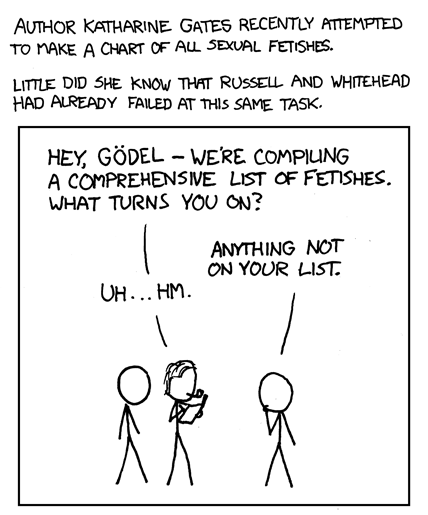
\includegraphics[height=5cm]{background/pix/xkcdfetishes.png}  \\
        \protect\label{fig:xkcdfetishes}\protect\href{https://xkcd.com/468/}{Courtesy XKCD}
      \protect\end{tabular}
    \protect\end{center}
  } % end boolean MakingPaperCopy
}。
\begin{equation*}
  R=\set{s \suchthat s\notin f(s)}
\end{equation*}
我们将证明定义域中没有元素映射到~$R$，因此 $f$ 不是满射。
假设存在 $\hat{s}\in S$ 使得 $f(\hat{s})=R$。
考虑 $\hat{s}$ 是否是~$R$ 的元素。
我们有 $\hat{s}\in R$ 当且仅当 $\hat{s}\in\set{s\suchthat s\notin f(s)}$。
根据~$R$ 的定义，这成立当且仅当 $\hat{s}\notin f(\hat{s})$，而这
又当且仅当 $\hat{s}\notin R$ 时成立。
这一矛盾意味着这样的 $\hat{s}$ 不存在。
\end{proof}


%</pf:CantorsThm>

%<*cor:FcnsNToNNotCountable>


\begin{corollary} \label{cor:FcnsNNGreaterFcnsN}
自然数集~$\N$ 的势严格小于自然数函数集~$\map{f}{\N}{\N}$ 的势。
也就是说，这样的函数有不可数多个。
\end{corollary}


%</cor:FcnsNToNNotCountable>

%<*pf:FcnsNToNNotCountable>


\begin{proof}
记函数集为~$G$。
存在一个从 $\powerset(\N)$ 到~$G$ 的一一映射，即把
每个子集 $S\subseteq\N$ 与其特征函数 $\map{\charfcn{S}}{\N}{\N}$ 相关联的映射。
因此 $\sizeof{\N}<\sizeof{\powerset(\N)}\leq\sizeof{G}$。
\end{proof}


%</pf:FcnsNToNNotCountable>

\begin{corollary}[不可计算函数的存在性]
存在一个函数 $\map{f}{\N}{\N}$，它不是可计算的：对所有~$e$，$f\neq\TMfcn_e$。
\end{corollary}

\begin{proof}
固定一个字母表。\footnotemark{} %
\zcref{co:SetOfTMsCountable}
表明，在这个字母表上，Turing 机是可数多的。
先前的结论表明，从 $\N$ 到自身的函数是不可数多的。
因此，Turing 机严格少于从 $\N$ 到自身的函数。
特别地，如果我们把每台 Turing 机与它计算的函数关联起来，
这个关联不是满射。
所以，存在一个自然数函数，没有 Turing 机能计算它。
\end{proof}

\footnotetext{%
  我们可以使用任意一个至少包含一个除空白符外字符的字母表，
  例如 $\Sigma=\set{\blank,\str{1}}$。
  在 Church 论题的讨论中，我们陈述过（尽管没有证明）
  在这种字母表上的 Turing 机能计算任何在其他字母表上可计算的函数。}

这是一个划时代的结果。
根据 Church 论题，\index{Church's Thesis!and uncountability}
我们以此证明存在一些计算机无法完成的工作。

%\footnote{%
  对于上过程序设计课的人来说，他们反复经历从任务到完成该任务的程序的转换，
  存在无法完成的事情可能令人惊讶，甚至震惊。
  这些结果的一个要点是，尽管这里关于无穷大小的工作
  起初可能显得过于抽象而不切实际，
  但它仍然能得出有趣且有用的结论。
%}

% ...............................................
\begin{exercises}


\begin{exercise}
\citetext{你的学习伙伴对对角化论证感到困惑}{%
  来自 \autocite{SE:Kaktus}.}。
  “如果你有一个无限长的列表，它显然包含所有的数字，对吧？
  我的意思是，如果你有一个真正‘无限’的列表，
  那你根本不可能找到一个不在列表上的数字！”
  帮他们理清思路。
\begin{answer}\verified
无限与穷尽是两回事。
列表 $0,2,4,\ldots$ 是无限的，但并没有穷尽所有自然数。
\end{answer}
\end{exercise}

\begin{exercise}
你的同学说：“教授，我搞糊涂了。
有一位小数的数构成的集合，比如 $25.4$ 和 $0.1$，显然是可数的——只需将整数的小数点全部左移一位即可。
有两位小数的集合，比如 $2.54$和 $6.02$，同样可数，以此类推。
这是可数多个集合，每个都可数，所以它们的并集是可数的。
这个并集就是全体实数，所以我认为实数是可数的。”
他们的错误在哪里？
\begin{answer}\verified
  这个并集并不是全体实数。
  它不包含无理数。
  例如，$\pi=3.14\ldots{}$ 不在任何一个集合中，因此也不在并集中。
  你的同学只考虑了末尾为零的数。
\end{answer}
\end{exercise}

\begin{exercise}
对下列有限集验证 Cantor 定理（\zcref{th:CantorsThm}）。
\begin{exparts*}
\item $\set{0,1,2}$
\item $\set{0,1}$
\item $\set{0}$
\item $\set{}$
\end{exparts*}
\begin{answer}\verified
Cantor 定理说幂集的元素个数比原集合多。
\begin{exparts}
\item 集合 $\set{0,1,2}$ 有三个元素，
它的幂集有八个元素。
\begin{equation*}
  \powerset(\set{0,1,2})=
  \set{\set{0,1,2},\; \set{0,1},\; \set{0,2},\; \set{1,2},\;
       \set{0},\; \set{1},\; \set{2},\; \emptyset}
\end{equation*}
\item 集合 $\set{0,1}$ 有两个元素，而它的幂集
$\powerset(\set{0,1})=\set{\set{0,1},\set{0},\set{1},\emptyset}$
有四个元素。
\item 集合 $\set{0}$ 只有一个元素，但它的幂集
$\powerset(\set{0})=\set{\set{0},\emptyset}$ 有两个元素。
\item 空集有零个元素，而它的幂集
$\powerset{\emptyset}=\set{\emptyset}$ 有一个元素。
\end{exparts}
\end{answer}
\end{exercise}

\recommended


\begin{exercise}
使用 \zcref{def:CardLessThanOrEqual} 证明第一个集合的势小于或等于第二个集合。
\begin{exparts}
\item $S=\set{1,2,3}$，$\hat{S}=\set{11,12, 13}$
\item $T=\set{0,1,2}$，$\hat{T}=\set{11,12, 13, 14}$
\item $U=\set{0,1,2}$，奇数集合
\item 偶数集合，奇数集合
\end{exparts}
\begin{answer}\verified
势的“$\leq$”定义是：如果存在一个从 $A$ 到~$B$ 的一一函数，
则 $\sizeof{A}\leq\sizeof{B}$。
\begin{exparts}
\item 函数 $\map{f}{S}{\hat{S}}$ 定义为 $f(1)=11$，$f(2)=12$，
$f(3)=13$，通过观察可知它是一一的。
\item 函数 $\map{f}{T}{\hat{T}}$ 定义为 $f(1)=11$，$f(2)=12$，
$f(3)=13$，通过观察可知它是一一的。
\item 同样通过观察，
函数 $\map{f}{U}{\mathbb{O}}$ 定义为 $f(1)=1$，$f(2)=3$，
$f(3)=5$，它是一一的。
\item
函数 $\map{f}{\mathbb{E}}{\mathbb{O}}$ 定义为 $f(x)=x+1$ 是一个一一函数。
验证很容易：$f(x_0)=f(x_1)$ 蕴含 $x_0+1=x_1+1$，
所以 $x_0=x_1$。
\end{exparts}
\end{answer}
\end{exercise}

\begin{exercise}
一个集合是可数的，另一个是不可数的。
哪个是哪个？
\begin{exparts*}
\item $\set{n\in\Z\suchthat n+3< 5}$
\item $\set{x\in\R\suchthat x+3< 5}$
\end{exparts*}
\begin{answer}
两者的区别在于元素所取自的集合不同。
\begin{exparts}
\item 集合 $S=\set{n\in\Z\suchthat n+3< 5}=\set{\ldots,-2,-1,0,1}$
  是可数的。
  由 $n\mapsto -n+1$ 定义的函数 $\map{f}{\N}{S}$ 是一个对应，这很容易验证。
\item 不可数；它是实数集 $\open{-\infty}{2}$。
  （在映射 $x\mapsto \ln(2-x)$ 下，此集合与 $\R$ 对应。）
\end{exparts}
\end{answer}
\end{exercise}

\recommended


\begin{exercise}
指出每个集合是可数的还是不可数的。
只需用一个词回答。
\begin{exparts*}
\item
$\open{5}{\infty}\subset\R$
\item
$\leftclosed{1}{4}\subset\N$
\item
$\leftclosed{1}{4}\subset\R$
\item
$\leftclosed{5}{\infty}\subset\N$
\end{exparts*}
\begin{answer}\verified
\begin{exparts}
\item 不可数。
  （函数 $x\mapsto\ln(x-5)$ 是与 $\R$ 的一个对应。）
\item 可数。
  （因为它是作为自然数的子集给出的，而且该集合是 $\set{1,2,3}$，是有限的。）
\item 此集合是不可数的。
  （集合 $S=\leftclosed{1}{4}\subset\R$ 的势至少与 $T=\open{1}{4}\subset\R$ 相同，
  因为由 $x\mapsto x$ 给出的包含映射 $\map{\iota}{T}{S}$ 是一一的。
  区间 $T$ 与 $\R$ 同势。
  一种理解方式是，从区间 $\open{-\pi/2}{\pi/2}$ 与 $\R$ 之间由 $x\mapsto \tan(x)$ 给出的对应出发。
  通过将该区间按 $\pi/3$ 的比例缩放然后再平移，使其适配定义域 $T$ 的情况，可得
  $x\mapsto \tan(\,(\pi/3)\cdot(x-1)-(\pi/2)\,)$ 是一个对应。）
\item 可数。
  （$\N$ 的任何子集都是可数的。）
\end{exparts}
\end{answer}
\end{exercise}

\begin{exercise}
列出所有定义域为 $A_2=\set{0,1}$、陪域为 $\powerset(A_2)$ 的函数。
对于一个有三个元素的集合 $A_3$，有多少个这样的函数？
$n$~个元素呢？
\begin{answer}\verified
对于二元集 $A_2=\set{0,1}$，其幂集，
$\powerset(A_2)=\set{\set{0,1},\, \set{0}, \set{1}, \set{}}$，
有四个元素。
构造一个从 $A_2$ 到 $\powerset(A_2)$ 的函数，需要指定将 $0$ 和 $1$ 映射到哪里。
因此有 $4^2=16$ 个不同的函数。
\begin{equation*}
\begin{array}{r|*{2}{c}}
  \multicolumn{1}{r}{\tabulartext{function~$f_i$}}
         &f_i(0)     &f_i(1)  \\
  \hline
  f_{0}  &\set{}     &\set{}  \\
  f_{1}  &\set{}     &\set{0}  \\
  f_{2}  &\set{}     &\set{1}  \\
  f_{3}  &\set{}     &\set{0,1}  \\
  f_{4}  &\set{0}    &\set{}  \\
  f_{5}  &\set{0}    &\set{0}  \\
  f_{6}  &\set{0}    &\set{1}  \\
  f_{7}  &\set{0}    &\set{0,1}  \
\end{array}
\hspace*{3em}
\begin{array}{r|*{2}{c}}
  \multicolumn{1}{r}{\tabulartext{function~$f_i$}}
         &f_i(0)     &f_i(1)  \\
  \hline
  f_{8}  &\set{1}    &\set{}  \\
  f_{9}  &\set{1}    &\set{0}  \\
  f_{10} &\set{1}    &\set{1}  \\
  f_{11} &\set{1}    &\set{0,1}  \\
  f_{12} &\set{0,1}  &\set{}  \\
  f_{13} &\set{0,1}  &\set{0}  \\
  f_{14} &\set{0,1}  &\set{1}  \\
  f_{15} &\set{0,1}  &\set{0,1}  \\
\end{array}
\end{equation*}

三元集 $A_3$ 有
$\sizeof{\powerset(A_3)}=8$。
从 $A_3$ 到 $\powerset(A_3)$ 的函数数量是 $8^3=512$。
一般而言，当 $\sizeof{A}=n$ 时，幂集有
$\sizeof{\powerset(A_3)}=2^n$ 个元素。
函数数量是 $(2^n)^n=2^{(n^2)}$。
（作为验证，$n=2$ 得到 $2^4=16$，
$n=3$ 得到 $2^9=512$。）
\end{answer}
\end{exercise}

\begin{exercise}
列出所有从 $S$ 到 $T$ 的函数。
哪些是一一的？
\begin{exparts*}
\item $S=\set{0,1}$, $T=\set{10,11}$
\item $S=\set{0,1}$, $T=\set{10,11,12}$
\end{exparts*}
\begin{answer}\verified
\begin{exparts}
\item 这些是从 $S$ 到 $T$ 的函数。
  \begin{equation*}
  \begin{array}{r|*{2}{c}}
    \multicolumn{1}{c}{\tabulartext{function $f_i$}}
          &f_i(0)  &f_i(1)  \\
    \cline{2-3}
    f_{0} &10      &10 \\
    f_{1} &10      &11 \\
    f_{2} &11      &10 \\
    f_{3} &11      &11 \\
  \end{array}
  \end{equation*}
  一一的函数是 $f_1$ 和 $f_2$。
\item 这些是从 $S$ 到 $T$ 的函数。
  \begin{equation*}
  \begin{array}{r|*{2}{c}}
    \multicolumn{1}{c}{\tabulartext{function $f_i$}}
          &f_i(0)  &f_i(1)  \\
    \hline
    f_{0} &10       &10 \\
    f_{1} &10       &11 \\
    f_{2} &10       &12 \\
    f_{3} &11       &10 \\
    f_{4} &11       &11 \\
  \end{array}
  \hspace{3em}
  \begin{array}{r|*{2}{c}}
    \multicolumn{1}{c}{\tabulartext{function $f_i$}}
          &f_i(0)  &f_i(1)  \\
    \hline
    f_{5} &11       &12 \\
    f_{6} &12       &10 \\
    f_{7} &12       &11 \\
    f_{8} &12       &12 \\
  \end{array}
  \end{equation*}
  一一的函数是 $f_1$、$f_2$、$f_3$、$f_5$、$f_6$
  和 $f_7$。
\end{exparts}
\end{answer}
\end{exercise}

\recommended


\begin{exercise}\begin{credit}
  \href{http://scherk.pbworks.com/w/page/14864221/Quiz%3A%20Countable%20sets}{User scherk at \texttt{pbworks.com}}.
\end{credit}
简答题：填空，从下列选项中选择可能的最强结论填入每个空格，
(i)~不可数，
(ii)~可数或不可数，
(iii)~有限，
(iv)~可数，
(v)~有限、可数无限或不可数
（同一答案可用于多个空格或完全不用）。
无需给出证明。
\begin{exparts}
\item 如果 $A$ 和 $B$ 是有限的，
那么 $A\cup B$ 是 \fillinblank。
\item 如果 $A$ 是可数的且 $B$ 是有限的，
那么 $A\cup B$ 是 \fillinblank。
\item 如果 $A$ 是可数的且 $B$ 是不可数的，
那么 $A\cup B$ 是 \fillinblank。
\item 如果 $A$ 是可数的且 $B$ 是不可数的，
那么 $A\cap B$ 是 \fillinblank。
\end{exparts}
\begin{answer}\verified
\begin{exparts}
\item 答案是~(iii)~有限，因为两个有限集的并集是有限的。
  （以下所有选项都成立：(ii)~可数或不可数，
  (iii)~有限，
  (iv)~可数，
  以及 (v)~有限、可数无限或不可数。
  但最强、最具体的是~(iii)。）
\item 最强的是~(iv)。
\item 最强的是~(i)。
\item 最强的是~(iv)。
  （交集可能是有限的，但也存在可数的情况，例如 $A=\N$ 和 $B=\R$。
  因此在一般情况下我们能做出的最强陈述是~(iv)。）
\end{exparts}
\end{answer}
\end{exercise}

\begin{exercise}
简答题：考虑 $\map{f}{S}{T}$，其中 $S$ 是可数的。
对于以下两项，列出所有可能成立的选项
(i)~$S$ 是有限的，
(ii)~$T$ 是有限的，
(iii)~$S$ 是可数无限的，
(iv)~$T$ 是可数无限的，
(v)~$T$ 是不可数的：
\begin{exparts*}
\item 该映射是满射的，
\item 该映射是一一的。
\end{exparts*}
\begin{answer}\verified
问题不要求证明，但这里的括号注释给出了理由。
\begin{exparts}
\item
  除最后一项外，其他都是可能的。
  （满足 (i) 和 (ii) 的一个例子是 $\map{\identity}{\set{0,1}}{\set{0,1}}$。
  满足 (iii) 和 (iv) 的一个例子是 $\map{\identity}{\N}{\N}$。
  \zcref{lem:CountableIffOntomap} 排除了 (v)。）
\item
  所有都是可能的。
  （满足 (i) 和 (ii) 的一个例子是 $\map{\identity}{\set{0,1}}{\set{0,1}}$。
  满足 (iii) 和 (iv) 的一个例子是 $\map{\identity}{\N}{\N}$。
  满足 (v) 的一个例子是由 $\iota(x)=x$ 给出的 $\map{\iota}{\N}{\R}$。）
\end{exparts}
\end{answer}
\end{exercise}

\begin{exercise}
\begin{credit}
   Math StackExchange 用户 Robert Z \url{https://math.stackexchange.com/a/1896328/12012}
\end{credit}
设 $S=\closed{0}{1}$ 和 $T=\open{0}{1}$ 是实数区间。
给出一个对应。
\hint~$f(x)=x$ 对大多数输入都有效，但端点必须映射到某个位置，所以
从 $f(0)=1/2$ 和 $f(1)=1/4$ 开始，并顺推下去。
\begin{answer}\verified
根据提示，考虑以下函数。
\begin{display}
  \begin{minipage}{0.5\textwidth}
    \begin{equation*}
      f(x)=
      \begin{cases}
        1/2  &\case{if $x=0$}  \\
        1/2^{n+2}  &\case{if $x=1/2^n$ for $n\in\N$}  \\
        x    &\case{otherwise}
      \end{cases}
    \end{equation*}
  \end{minipage}
  \quad
  \vcenteredhbox{
\includegraphics{\asydir correspondences/correspondences005.pdf}}
\end{display}
论证函数 $f$ 是一一的且满射的一种方法是看它满足水平线测试，
即对于每个 $t\in\open{0}{1}$，水平线 $y=t$ 都恰好有一个对应的输入 $x$。

我们可以展开说明。
首先考虑输出 $y\in\open{0}{1}$ 满足 $y\neq 1/2^n$（$n\in\N^+$）的情况。
那么 $y$ 恰好有一个对应的输入，即 $x=y$。
另一种情况是对某个 $n\in\N^+$ 有 $y=1/2^n$。
这里也有且仅有一个对应的输入 $x$。
具体来说，如果 $n=1$，那么输入是 $x=0$，它在定义域
$\closed{0}{1}$ 中。
如果 $n> 1$，那么输入是 $x=1/2^{n-2}$，它也是 $\closed{0}{1}$ 中的一个元素。
\end{answer}
\end{exercise}

\recommended


\begin{exercise}
给出一个势大于 $\R$ 的集合。
\begin{answer}\verified
\zcref{th:CantorsThm} 说对于任意集合，
其势严格小于其幂集的势。
所以一个势大于 $\R$ 的集合是 $\powerset(\R)$。
（另一个是 $\powerset(\powerset(\R))$。）
\end{answer}
\end{exercise}

\recommended


\begin{exercise}
回忆我们将比特的集合记为 $\B=\set{0,1}$。
\begin{exparts}
\item
证明有限比特串的集合，
$\sequence{b_0b_1\ldots\, b_{k-1}}$（其中 $b_i\in\B$ 且 $k\in\N$），
是可数的。
\item
我们可以将无限比特串 $f=\sequence{b_0,b_1,\ldots}$ 视为函数 $\map{f}{\N}{\B}$。
使用对角化证明无限比特串的集合
是不可数的。
\end{exparts}
\begin{answer}\verified
\begin{exparts}
\item 有限比特串的集合 $\kleenestar{\B}\!$，是集合
  $\B^k=\set{\sequence{b_0b_1\ldots\, b_{k-1}}\suchthat k\in\N}$ 的并集。
  集合 $\B^k$ 是有限的，因为它有 $2^k$~个元素
  （当 $k=0$ 时，它只包含空串），所以
  这是可数多个可数集合的并集。
\item
  假设我们可以对无限比特串的集合进行计数，
  即它有一个穷举枚举 $f_0, f_1, \ldots$\sentencespace
  令 $\map{g}{\B}{\B}$ 由 $g(0)=1$ 和
  $g(1)=0$ 给出。
  那么由 $F(i)=g(f_i(i))$ 定义的无限比特串 $\map{F}{\N}{\B}$ 不等于
  任何一个 $f_i$，
  这与该枚举是穷举的相矛盾。
\end{exparts}
\end{answer}
\end{exercise}

\begin{exercise}
证明对于两个集合，$S\subseteq T$ 蕴含 $\sizeof{S}\leq \sizeof{T}$。
\begin{answer}\verified
设 $S$ 和 $T$ 满足 $S\subseteq T$。
那么包含映射，即由 $\iota(s)=s$ 给出的映射 $\map{\iota}{S}{T}$，
显然是一一的。
所以由 \zcref{def:CardLessThanOrEqual}，$\sizeof{S}\leq \sizeof{T}$。
\end{answer}
\end{exercise}

\begin{exercise}
用对角化方法证明以下命题为假：所有值域有限的函数~$\map{f}{\N}{\N}$ 都是可计算的。
\hint~只需证明这类函数的集合是不可数的。
\begin{answer}\verified
我们遵照提示。
将所有这样的函数组成的集合记作$S=\set{\map{f}{\N}{\N}\suchthat \text{$\range(f)$ is finite}}$。
假设 $S$ 是可数的，从而存在一个对应 $\map{h}{\N}{S}$。
对于所有自然数~$i$，$h(i)$ 的值是一个函数，我们将其记作~$f_i$。

定义映射 $\map{g}{\N}{\N}$：若 $x\neq 0$ 则 $g(x)=0$，否则 $g(x)=1$。
考虑由$k(i)=g(\,f_i(i)\,)$给出的函数 $\map{k}{\N}{\N}$。
这个映射的值域是有限的，即$\range(k)=\set{0,1}$，但 $k$ 不等于 $S$ 中的任何一个~$f_i$，因为它们在输入~$i$ 处的取值不同。
\end{answer}
\end{exercise}

% \begin{exercise}
% Given a countable number of nonempty sets, $S_i\neq\emptyset$ for
% $i\in\N$,
% show that their product
% $S_0\times S_1\times \cdots$ is uncountable.
% \begin{answer} % Requires countable choice https://math.stackexchange.com/a/500855
% Let $T=S_0\times S_1\times \cdots$ where each $S_i$ is nonempty.
% Clearly $T$ is infinite.
% We will show that no map $\map{f}{\N}{T}$ is onto.

% Recall that the characteristic function of $S_i$ is denoted $\charfcn(S_i)$.
% Let $g$ be the map on $\B=\set{0,1}$ given by
% $g(b)=1-b$, which is $g(0)=1$ and $g(1)=0$.

% Now consider the set whose characteristic function is
% $g(\charfcn(S_i)(i))$.
% Then for all~$i$, $z\neq f(i)$ because $z[i]\neq f(i)[i]$.
% So $f$ is not onto.
% \end{answer}
% \end{exercise}

% No way to make an exercise? https://math.stackexchange.com/a/183383/12012
% \begin{exercise}
% You study with someone who says,
% ``Yes, obviously there are different sizes of infinity.
% The plane $\R^2$ obviously has infinitely many more points then the
% line~$\R$, so it is a larger infinity.''
% Convince them that
% their argument is wrong because the cardinality of the plane is the same
% as the cardinality of the line.
% \hint~consider the function $\map{f}{\R^2}{\R}$ such that $f(x,y)$ interleaves
% the digits of the two input numbers.
% \end{exercise}

\begin{exercise}
在数学课上，我们主要处理有理数，这可能给人留下无理数不常见的印象。
但实际上，无理数比有理数更多。
证明：根据 \zcref{ex:RationalsAreCountable}，虽然有理数集是可数的，但无理数集是不可数的。
\begin{answer}\verified
\zcref{ex:RationalsAreCountable} 表明有理数集是可数的。
假设无理数集也是可数的。
那么由于两个可数集的并集是可数的，实数集将是可数的。
但实数集是不可数的，因此无理数集也不可数。
\end{answer}
\end{exercise}

\recommended


\begin{exercise}
\zcref{ex:RationalsAreCountable} 表明有理数是可数的。
如果我们将 \zcref{th:RealsNotCountable} 中给出的对角线论证应用到有理数的一个枚举上，会发生什么？
考虑一个包含所有有理数的序列 $q_0, q_1,\ldots$。
用小数展开式 $q_i=d_i.d_{i,0}d_{i,1}d_{i,2}\ldots$（其中 $d_i\in\Z$ 且$d_{i,j}\in\set{0,\ldots 9}$）表示每个这样的数，该展开式不以全~$9$ 结尾，从而保证小数展开式是唯一的。
\begin{exparts}
\item
  设 $g$ 是定义在十进制数字 $0,1,\ldots{} 9$ 上的映射，满足 $g(1)=2$，且当 $i\neq 2$ 时 $g(i)=1$。
  考虑对角线上的数$d=\sum_{n\in\N}d_{n,n}\cdot 10^{-(n+1)}\!$。
  用~$g$ 变换其各位数字，即定义$z=\sum_{n\in\N}g(d_{n,n})\cdot 10^{-(n+1)}\!$。
  证明 $z$ 是无理数。
\item 利用前一小题得出结论：对角线上的数 $d=\sum_{n\in\N}d_{n,n}\cdot 10^{-(n+1)}$ 是无理数。
  \hint~证明它的小数展开式没有重复模式。
\item
  为什么对角线上的数不是有理数这一事实，与我们能够枚举所有有理数这一事实不矛盾？
\end{exparts}
\begin{answer}\verified
\begin{exparts}
\item
  将 $z$ 的小数展开式写成~$z=0.z_0z_1z_2\ldots$\sentencespace
  由于 $g$ 的输出永远不会是~$9$，所以 $z$ 的小数展开式不以 $9$ 结尾。
  因此 $z$ 有唯一的小数展开式。
  对于每个~$q_i$，$z$ 的小数展开式与 $q_i$ 的不同之处在于$z_{i}\cdot 10^{-(i+1)}\neq q_{i,i}\cdot 10^{-(i+1)}$，
  这是由~$g$ 的定义决定的。
  因为它们的小数展开式不同，并且都不以 $9$ 结尾，所以它们是不同的数。

  由于 $z$ 不等于任何有理数，所以它是无理数。
\item
  如果$d=\sum_{n\in\N}d_{n,n}\cdot 10^{-(n+1)}$是有理数，那么它的小数展开式会循环。
  也就是说，存在一个小数位，使得从该位之后，展开式由一串数字$d_{j}d_{j+1}\ldots\, d_{j+k}$不断重复组成。
  但这样一来，前一小题中的~$z$ 也会循环，即从同一个小数位之后，它的展开式将由一串数字$g(d_{j})g(d_{j+1})\ldots\, g(d_{j+k})$不断重复组成。
  这将使得~$z$ 成为有理数，但 $z$ 并不是。
\item
  在 \zcref{th:RealsNotCountable} 中，我们从一个声称包含所有实数的列表开始，然后构造出一个不在该列表中的实数。
  这里，我们从一个包含所有有理数的列表开始，构造出了一个不是有理数的数。
  这使得它仍然是一个实数，只不过不是有理实数。
\end{exparts}
\end{answer}
\end{exercise}

\begin{exercise}
通过证明若 $S$ 有限，则其幂集的势是 $\sizeof{\powerset(S)}=2^{\sizeof{S}}$，来验证 Cantor 定理在有限情况下成立。
\begin{answer}\verified
在证明之前，作为归纳步骤的启发，考虑 $S=\set{0,1,2,3}$。
这些是 $\powerset(S)$ 的十六个元素。
第一行是不包含~$3$ 的集合，而第二行是包含~$3$ 的集合。
\begin{equation*}
\begin{array}{*{8}{c}}
  \set{},  &\set{0},   &\set{1},   &\set{2},   &\set{0,1},   &\set{0,2},   &\set{1,2},   &\set{0,1,2}, \\
  \set{3}, &\set{0,3}, &\set{1,3}, &\set{2,3}, &\set{0,1,3}, &\set{0,2,3}, &\set{1,2,3}, &\set{0,1,2,3}
\end{array}
\end{equation*}
底行的每个集合与顶行匹配的集合相同，只是多加了一个~$3$。

我们通过对 $\sizeof{S}$ 进行归纳来证明。
基本情况是 $\sizeof{S}=0$，即 $S$ 是空集。
那么 $\powerset(S)=\set{\emptyset}$ 且 $\sizeof{\powerset(S)}=1=2^0\!$，符合要求。

对于归纳步骤，固定 $k\in\N^+\!$，假设命题对 $n=0$，$n=1$，\ldots{} $n=k$ 成立，并考虑一个集合 $S$ 满足 $\sizeof{S}=k+1$。
因为 $\sizeof{S}=k+1$，集合~$S$ 至少有一个元素 $\hat{s}\in S$。
对 $S-\set{\hat{s}}$ 应用归纳假设可知，$\powerset(S-\set{\hat{s}})$ 有 $2^k$ 个元素。
如上所示，$\powerset(S)$ 中不包含 $\hat{s}$ 的元素与 $\powerset(S)$ 中包含~$\hat{s}$ 的元素一一对应。
但是 $\powerset(S)$ 中不包含~$\hat{s}$ 的集合正是 $\powerset(S-\set{\hat{s}})$ 中的集合。
因此，$\powerset(S)$ 的元素总数是 $2\cdot 2^k$，等于 $2^{k+1}\!$。
\end{answer}
\end{exercise}

\begin{exercise}
\begin{credit}
  \href{https://viterbi-web.usc.edu/~mjneely/docs/infinity.pdf}{Michael J~Neely }
\end{credit}
\zcref{th:RealsNotCountable} 中 Cantor 定理证明的关键是 $R=\set{s\suchthat s\notin f(s)}$ 的定义。
这个故事阐明了这个思想：高中年鉴要求每个毕业生~$s_i$ 列出一个他们认为将来会成名的班级成员名单 $f(s_i)$。
定义谦逊学生集合~$H$ 由那些不在自己名单上的学生组成。
证明没有学生的名单等于~$H$。
\begin{answer}\verified
假设 $f(s_i)=H$。
我们将论证 $s_i\in H$ 和 $s_i\notin H$ 都不成立。
如果 $s_i\in H$，那么学生~$s_i$ 是自己名单上的一员，因此根据谦逊的定义，$s_i$ 不谦逊，这与该情况下的假设矛盾。
另一方面，如果 $s_i\notin H$，那么 $s_i$ 不在自己名单上，因此 $s_i$ 是谦逊的，这与该情况下的假设矛盾。
\end{answer}
\end{exercise}

\begin{exercise}
证明不存在所有集合的集合。
\hint~使用 \zcref{th:CantorsThm}。
\begin{answer}\verified
  假设相反，即 $\mathcal{C}$ 是所有集合的集合。
  那么 $\powerset(\mathcal{C})$ 将是一个集合的集合，因此我们将有 $\powerset(\mathcal{C})\subseteq \mathcal{C}$。
  这将导致 $\sizeof{\powerset(\mathcal{C})}\leq\sizeof{\mathcal{C}}$，从而与 Cantor 定理矛盾。
\end{answer}
\end{exercise}

\begin{exercise}
\zcref{th:RealsNotCountable} 的证明必须处理某些十进制数有不止一种表示的事实。
二进制也具有某些数不止一种表示的性质；例如 $0.01000\ldots$ 和 $0.00111\ldots$。
但在二进制的论证中，构造~$z$ 时无法避免数字~$0$ 和~$1$。
如何使该论证在二进制下成立？
\begin{answer}\verified
一种方法是每次取两个对角线位；例如将 $01$ 改为 $10$，并将任何其他两位序列改为 $01$。
\end{answer}
\end{exercise}

\begin{exercise}
\begin{credit}
  答案由 Stack Exchange 用户\footnote{\url{https://math.stackexchange.com/a/271126}} Alex Becker 提供。
\end{credit}
在 \zcref{th:RealsNotCountable} 的陈述之后的讨论中提到，实数~$1$ 有两种小数表示：$1.000\ldots=0.999\ldots$\sentencespace
\begin{exparts}
\item
使用无限几何级数的公式验证这个等式，$a+ar+ar^2+ar^3+\cdots =a/(1-r)$。
\item
证明如果一个数有两种不同的小数表示，那么在它们最左边不同的那个小数位上，它们的数字恰好相差~$1$。
\hint 提示：余下的小数位所能弥补的最大差值就是这个数。
\item
此外，证明在首次不同的数位上数字较大的那种表示中，其右边所有数位上的数字都是~$0$；而另一种表示中，所有余下数位上的数字都是~$9$。% \hint~this is similar to the prior item.
\end{exparts}
\begin{answer}\verified
在这个原型 $1.000\ldots=0.999\ldots$ 中，我们将两种表示写作
$x_0=1$，$x_{-1}=0$，$x_{-2}=0$，……，和
$y_0=0$，$y_{-1}=9$，$y_{-2}=9$，……\sentencespace
注意，这些下标（即小数位）是像 $0$ 和~$-1$ 这样的整数，并非自然数。
\begin{exparts}
\item
在$a+ar+ar^2+ar^3+\cdots =a/(1-r)$中，令 $a=9$ 且 $r=0.1$。
左边是$9+0.9+0.09+0.009+\cdots=9.999\,99\ldots$\sentencespace
右边是$9/(1-(0.1))=9/0.9=10$。
两边减去~$9$ 可得 $0.999\,99\ldots=1$。
\item
考虑一个有两种表示的实数。
在这两种表示中存在一个最左边的非零小数位 $N\in\Z$。
因此，将这两种表示写为$\vec{x}=\sequence{x_N,x_{N-1},\ldots}$ 和
$\vec{y}=\sequence{y_N,y_{N-1},\ldots}$。
它们需要满足条件$x_i,y_i\in\set{0,1,\ldots 9}$，并且加起来等于同一个数。
\begin{equation*}
  \sum_{i\leq N}x_i\cdot 10^i=\sum_{i\leq N}y_i\cdot 10^i
  \tag{$*$}
\end{equation*}

将 ($*$) 改写成差值形式。
\begin{equation*}
  0=\bigl(\sum_{i\leq N}x_i\cdot 10^i\bigr)-\bigl(\sum_{i\leq N}y_i\cdot 10^i\bigr)
   =\sum_{i\leq N}(x_i-y_i)\cdot 10^i
\end{equation*}
设 $\vec{x}$ 和 $\vec{y}$ 首次不同的最左小数位为第~$M$ 位，
即对于 $i\in\set{N,N-1,\ldots\, M+1}$ 有 $x_i=y_i$，且 $x_M\neq y_M$。
$x_M$ 和~$y_M$ 其中一个大；不妨设 $x_M>y_M$。
去掉前面的零后，现在差值从第 $M$ 位开始。
\begin{equation*}
  0
   =\sum_{i\leq M}(x_i-y_i)\cdot 10^i
   =(x_M-y_M)\cdot 10^M+\sum_{i\leq (M-1)}(x_i-y_i)\cdot 10^i
  \tag{$**$}
\end{equation*}
我们在等式右边单独列出了第一项，因为我们需要证明 $x_M=y_M+1$
（正如原型中$\vec{x}=\sequence{1,0,0,\ldots}$和
$\vec{y}=\sequence{0,9,9,\ldots}$的情况那样）。
考虑余下的部分，$\sum_{i\leq (M-1)}(x_i-y_i)\cdot 10^i\!$。
为了使总和为零，这个尾部必须抵消$(x_M-y_M)\cdot 10^M\!$，
由于 $x_M>y_M$，这是一个正值。
尾部所能提供的最大抵消量出现在每个 $x_i-y_i$ 都等于~$-9$ 时。
几何级数公式给出了这个最大值。
\begin{equation*}
  -9\cdot 10^{M-1}-9\cdot 10^{M-2}+\cdots
  =-9\cdot 10^{M-1}\cdot\bigl[ 1+\frac{1}{10}+\frac{1}{100}+\cdots\bigr]  \\
  =\frac{-9\cdot 10^{(M-1)}}{1-(1/10)}=\frac{-9\cdot 10^{(M-1)}}{9/10}=-10^{M}
\end{equation*}
因此 $x_M-y_M=1$，因为尾部无法抵消更大的差值。
\item
再次考虑上一项的 ($**$)，既然我们已经证明了 $x_M-y_M=1$。
\begin{equation*}
  0
   =1\cdot 10^M+\sum_{i\leq (M-1)}(x_i-y_i)\cdot 10^i
\end{equation*}
我们想要证明每个 $x_i-y_i$ 都等于~$-9$。
我们只处理 $i=M-1$ 的情况，因为其他情况与此非常类似。

如果$x_{M-1}-y_{M-1}\geq -8$，那么 ($**$) 变为：
\begin{align*}
  0
   &=1\cdot 10^M+(x_{M-1}-y_{M-1})\cdot 10^{(M-1)}+\sum_{i\leq (M-2)}(x_i-y_i)\cdot 10^i
     \\
   &\geq 10\cdot 10^{(M-1)}-8\cdot 10^{(M-1)}+\sum_{i\leq (M-2)}(x_i-y_i)\cdot 10^i \\
   &=2\cdot 10^{(M-1)}+\sum_{i\leq (M-2)}(x_i-y_i)\cdot 10^i
\end{align*}
与上一项类似，为了使整个和为负，尾部必须抵消第一项。
通过令每个 $x_i-y_i$ 为 $-9$，可以得到最大的尾部。
再次应用无限几何级数的求和公式。
\begin{equation*}
  -9\cdot 10^{M-2}-9\cdot 10^{M-3}+\cdots
  =-9\cdot 10^{M-2}\cdot\bigl[ 1+\frac{1}{10}+\frac{1}{100}+\cdots\bigr]  \\
  =\frac{-9\cdot 10^{(M-2)}}{1-(1/10)}=\frac{-9\cdot 10^{(M-2)}}{9/10}=-10^{M-1}
\end{equation*}
尾部不足以抵消$2\cdot 10^{(M-1)}$，所以
$x_{M-1}-y_{M-1}\geq -8$ 是不可能的。
\end{exparts}
\end{answer}
\end{exercise}

\begin{exercise} \label{exer:SchroderBernstein}
\zcref{def:CardLessThanOrEqual} 将等势的定义推广为：如果存在从 $A$ 到 $B$ 的一一函数，则 $\sizeof{A}\leq \sizeof{B}$。
\definend{Schröder–Bernstein 定理} 指出，如果同时有 $\sizeof{S}\leq \sizeof{T}$ 和 $\sizeof{T}\leq \sizeof{S}$，那么 $\sizeof{S}=\sizeof{T}$。
我们将逐步讲解这个证明。
它依赖于寻找像的链：对于任意 $s\in S$，我们通过反复应用这两个函数（既向右也向左）来形成与之关联的链，如下所示。
\begin{equation*}
  \ldots{}\;f^{-1}(g^{-1}(s)),\,g^{-1}(s),\,s,\,f(s),\,g(f(s)),\,f(g(f(s)))\; \ldots{}
  % \tag{$*$}
\end{equation*}
（从 $s$ 开始，向右的链是
$s,\,f(s),\,g(f(s)),\,f(g(f(s))), \ldots$，而向左延伸的链是 $\ldots{}\,f^{-1}(g^{-1}(s)),\,g^{-1}(s),\,s$。）
对于任意 $t\in T$，类似地定义关联的链。

举一个例子：取整数集合 $S=\set{0,1,2}$ 和字符集合 $T=\set{\str{a},\str{b},\str{c}}$，
并考虑这里给出的两个一一函数 $\map{f}{S}{T}$ 和 $\map{g}{T}{S}$。
\begin{center}
  \begin{tabular}{c|c}
    $s$    &\multicolumn{1}{c}{$f(s)$}  \\ \hline
    $0$    &$\str{b}$  \\
    $1$    &$\str{c}$  \\
    $2$    &$\str{a}$
  \end{tabular}
  \qquad
  \vcenteredhbox{\includegraphics{\asydir maps/maps03.pdf}}
  \qquad
  \begin{tabular}{c|c}
    $t$       &\multicolumn{1}{c}{$g(t)$}  \\ \hline
    $\str{a}$ &$0$   \\
    $\str{b}$ &$1$    \\
    $\str{c}$ &$2$
  \end{tabular}
\end{center}
从 $0\in S$ 出发会得到一条循环链，
$\ldots{}\,0,\str{b},1,\str{c},2,\str{a},0\,\ldots$\sentencespace
\begin{exparts}
\item
  考虑 $S=\set{0,1,2,3}$ 和 $T=\set{\str{a},\str{b},\str{c},\str{d}}$。
  令 $f$ 关联 $0\mapsto\str{a}$，$1\mapsto\str{b}$，$2\mapsto\str{d}$
  以及 $3\mapsto\str{c}$。
  令 $g$ 关联 $\str{a}\mapsto 0$，$\str{b}\mapsto 1$，$\str{c}\mapsto 2$
  以及 $\str{d}\mapsto 3$。
  验证这些映射是一一的。
  列出每个 $S$ 中元素关联的链以及每个 $T$ 中元素关联的链。
\item 对于无限集合，一条链可以有一个首元素，即一个没有任何原像的元素。
  令 $S$ 为偶数集，$T$ 为奇数集。
  令 $\map{f}{S}{T}$ 为 $f(x)=x+1$，令 $\map{g}{T}{S}$ 为 $g(x)=x+1$。
  证明每个映射都是一一的。
  证明只存在一条链，并且该链有一个首元素。
\item 论证我们可以不失一般性地假设 $S$ 和 $T$ 是不相交的集合。
\item 假设 $S$ 和 $T$ 不相交，且 $\map{f}{S}{T}$ 和 $\map{g}{T}{S}$ 是一一的。
  证明这两个集合中的每个元素都在唯一的一条链中，并且每条链属于以下四种类型之一：
  (i) 那些在有限项后重复的链；
  (ii) 那些在两个方向上无限延伸且不重复的链；
  (iii) 那些向右无限延伸但在左边停止于 $S$ 的某个元素的链；
  (iv) 那些向右无限延伸但在左边停止于 $T$ 的某个元素的链。
\item 证明对于任意链，下面的函数是链中来自 $S$ 的元素与来自 $T$ 的元素之间的一个对应。
  \begin{equation*}
    h(s)=
    \begin{cases}
      f(s) &\case{if $s$ is in a sequence of type~(i), (ii), or~(iii)}  \\
      g^{-1}(s) &\case{if $s$ is in a sequence of type~(iv)}
    \end{cases}
  \end{equation*}
\end{exparts}
\begin{answer}\verified
\begin{exparts}
\item 这些是 $S$ 的链。
\begin{equation*}
\begin{array}{r|c}
  \multicolumn{1}{r}{s\in S}
  &\text{\makebox[2in][c]{\tabulartext{Chain}}}  \\ \hline
  0 &  \ldots\,0,\str{a},0,\str{a}\,\ldots   \\
  1 &  \ldots\,1,\str{b},1,\str{b}\,\ldots    \\
  2 &  \ldots\,2,\str{d},3,\str{c},2,\str{d}\,\ldots\\
  3 &  \text{---\,与 $2$ 的链相同\,---}
\end{array}
\end{equation*}
这些是 $T$ 的链。
\begin{equation*}
\begin{array}{r|c}
  \multicolumn{1}{r}{t\in T}
  &\text{\makebox[2in][c]{\tabulartext{Chain}}}  \\ \hline
  \str{a} &  \ldots\,\str{a},0,\str{a},0\,\ldots   \\
  \str{b} &  \ldots\,\str{b},1,\str{b},1\,\ldots    \\
  \str{c} &  \ldots\,\str{c},2,\str{d},3,\str{c},2\,\ldots\\
  \str{d} &  \text{---\,与 \str{c} 的链相同\,---}
\end{array}
\end{equation*}

\item % As the question asks we take
% $S=\set{0,2,4,6,\ldots}$, and $T=\set{1,3,5,\ldots}$,
% and take $\map{f}{S}{T}$ to be $f(s)=s+1$, and also take
% $\map{g}{T}{S}$ to be $g(t)=t+1$.
函数 $f$ 是一一的，因为如果 $f(s)=f(\hat{s})$，那么 $s+1=\hat{s}+1$，因此 $s=\hat{s}$。
函数 $g$ 同理也是一一的。

与 $0\in S$ 关联的链是 $0,1,2,3\ldots$\sentencespace
它包含两个集合的所有元素，因此该链是唯一的。
它还有一个首元素，即 $T$ 中没有元素是 $g^{-1}(0)$。

\item 如果它们尚未不相交，即 $S\cap T\neq\emptyset$，那么我们只需将 $S$ 的所有元素涂成绿色，将 $T$ 的所有元素涂成金色，就能使它们变得不相交。
更精确地说，考虑集合 $\set{0}\times S$（即形如 $\sequence{0,s}$ 的对）和集合 $\set{1}\times T$（即形如 $\sequence{1,t}$ 的对）。
因为来自不同集合的任意两个元素在第一项上不同，所以这两个集合是不相交的。

显然，它们对应于原始集合 $S$ 和 $T$。
因此，我们可以将结果重新表述为不相交的版本：如果同时有
$\sizeof{\set{0}\times S}\leq \sizeof{\set{1}\times T}$
和 $\sizeof{\set{1}\times T}\leq \sizeof{\set{0}\times S}$，
那么 $\sizeof{\set{0}\times S}=\sizeof{\set{1}\times T}$。

\item 首先证明每个元素都在一个唯一的链中。
固定某个 $x\in S\cup T$。
由于我们假设这两个集合不相交，所以作用于 $x$ 的函数运算是确定的，即如果 $x\in S$，那么在链中我们接下来考虑 $f(x)$；如果 $x\in T$，那么我们接下来考虑 $g(x)$。
由此，链中 $x$ 右侧的所有元素就确定了。
而且，由于这两个函数都是一一的，左侧的所有元素也同样确定了。

至于这四种可能性，一条链要么是有限的（即会重复），要么是无限的。
如果它重复，则属于情况 (i)。
如果它是无限的，那么它要么没有起始元素（因此属于情况 (ii)），要么有。
如果它有起始元素，那么该元素要么来自集合 $S$（如情况 (iii)），要么来自集合 $T$（如情况 (iv)）。

\item
下面我们将针对每种链类型考虑其对应关系。
但首先注意，因为每种情况都是使用函数 $f$ 和 $g$ 的限制来定义 $h$，所以在每种情况下 $h$ 都是良定义的。
也就是说，这些映射都不会将同一个输入关联到两个不同的输出。

类型 (i) 的链在 $n$ 个元素后重复，
$s_0,t_0,s_1,t_1,\ldots,s_{n-1},t_{n-1},s_n=s_0$
其中 $n>0$。
（它不能在单个元素后重复——不可能有 $s_0=t_0$——因为集合 $S$ 和 $T$ 不相交。）
因此，我们可以取这个循环中的第一个元素为 $S$ 的成员。
% So this is the chain, with $s=s_0$.
% \begin{equation*}
%   s,f(s),g(f(s)),f(g(f(s))),\ldots{} g(f(\,\cdots f(s)))=s
% \end{equation*}
函数 $f$ 建立如下关联。
\begin{equation*}
  s_0\mapsto t_0\quad s_1\mapsto t_1,\quad\ldots\quad s_{n-1}\mapsto t_{n-1}
\end{equation*}
这显然构成了链中元素之间的一个对应。
它显然满射到集合 $\set{t_0,t_1,\ldots t_{n-1}}$，且是一一的，因为各个 $t_j$ 互不相同，否则链会更短。

类型 (iii) 的链
\begin{equation*}
  s,\,f(s),\,g(f(s)),\,f(g(f(s))),\, \ldots{}
\end{equation*}
将偶数索引的项与奇数索引的项相关联。
\begin{equation*}
  s\mapsto f(s)\quad
  g(f(s))\mapsto f(g(f(s))),\quad\ldots
\end{equation*}
也就是说，我们将 $h$ 定义为将 $S$ 的成员映射到 $T$ 的成员。显然这是一个对应。

类型 (ii) 的链是类似的。
\begin{equation*}
  \ldots{}\,f^{-1}(g^{-1}(s)),\,g^{-1}(s),\,s,\,f(s),\,g(f(s)),\,f(g(f(s))),\, \ldots{}
  % \tag{$*$}
\end{equation*}
函数 $h$ 遵循 $f$ 的作用建立如下关联。
\begin{equation*}
  \ldots\quad
  f^{-1}(g^{-1}(s))\mapsto g^{-1}(s)\quad
  s\mapsto f(s)\quad
  g(f(s))\mapsto f(g(f(s))),\quad\ldots
\end{equation*}
这个关联显然也是一个对应。

需要稍加思考的是类型 (iv) 的链。
\begin{equation*}
  t,\,g(t),\,f(g(t)),\,g(f(g(t)),\, \ldots{}
\end{equation*}
我们希望对应函数 $h$ 从 $S$ 映射到 $T$。
考虑如下关联。
\begin{equation*}
  g(t)\mapsto t\quad
  g(f(t))\mapsto f(t),\quad\ldots
\end{equation*}
由于函数 $g$ 是一一的，其逆函数在其值域上有定义。
因此，用这些关联来定义 $h$ 便得到一个良定义的函数。
与上面的链类型类似，这显然也是一个对应。
\end{exparts}
\end{answer}
\end{exercise}

\end{exercises}
\index{cardinality|)}

\index{diagonalization|)}

%================================================
\section{通用性}\index{universality|(}

我们已经见过不少 Turing 机，例如输出为其输入的后继的机器，
将两个输入数相加的机器，等等。
这些都是单一用途的设备，要想获得不同的输入-输出行为，
我们就需要一台新的机器。
这张照片展示了早期计算机的程序员。\index{programmer}
他们正在用接线改变电路，从而改变机器的行为，
这本质上是在制造新的硬件。
% \begin{center}  \small
%   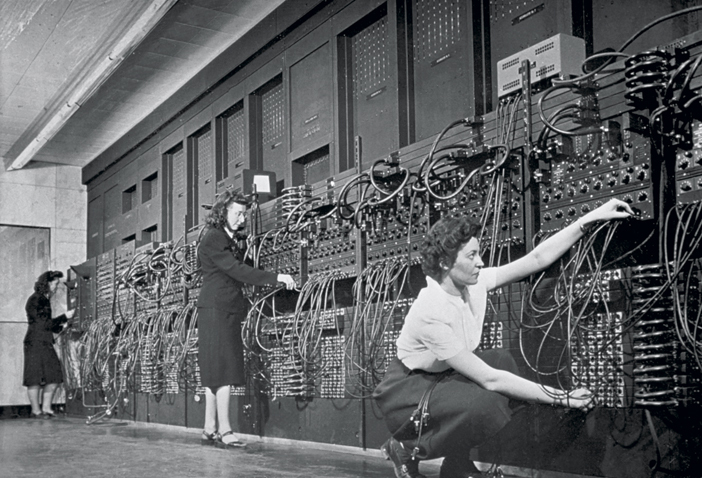
\includegraphics[width=.53\textwidth]{background/pix/rewiring.jpg} \\
%   \begin{credit}
%     \textit{ENIAC Programmers, 1946} \href{https://artsandculture.google.com/asset/eniac-programmers-united-states-army-united-states-army/4AFgcMwMqg1mRw}{U. S. Army Photo from Army Research Labs Technical Library}
%     % (US government works not subject to copyright.)
%   \end{credit}
%   \captionof{figure}{\protect\citetext{ENIAC, reconfigure by rewiring.}{Jean Jennings (left), Marlyn Wescoff (center), and Ruth Lichterman program the ENIAC, circa 1946. U. S. Army Photo}}
% \end{center}


\begin{fig}[eniac]{\protect\citetext{ENIAC，通过重新接线来重新配置。}{照片中，Jean Jennings（左）、Marlyn Wescoff（中）和 Ruth Lichterman 正在为 ENIAC 编程，约1946年。美国陆军照片。}}  \small
  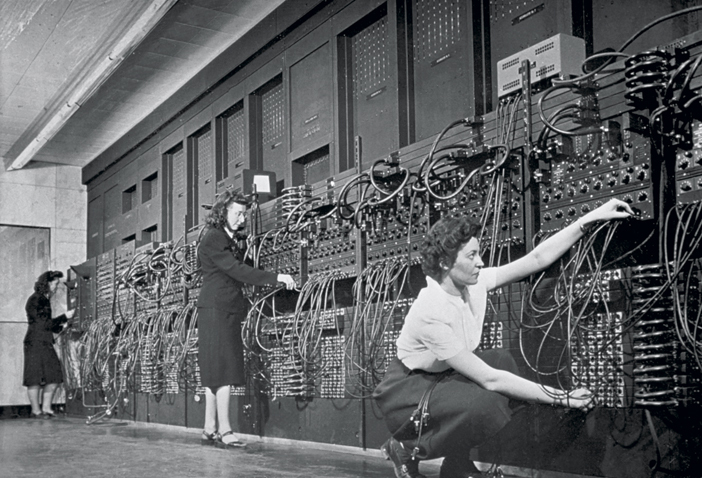
\includegraphics[width=.53\textwidth]{background/pix/rewiring.jpg} \\
  \begin{credit}
    \textit{ENIAC 程序员，1946} \href{https://artsandculture.google.com/asset/eniac-programmers-united-states-army-united-states-army/4AFgcMwMqg1mRw}{U. S. Army Photo from Army Research Labs Technical Library}
    % (US government works not subject to copyright.)
  \end{credit}
\end{fig}


\noindent 想象一下，你有一部手机，当你想从运行浏览器切换到接电话时，
必须拔下一块芯片并换上另一块。\index{hardware}
图中的接线方式比起电烙铁来已经是一种改进，但这还不是最终的答案。
% We want our machines to have their behavior changed by software, not hardware.

\subsection{通用 Turing 机}\index{Universal Turing machine|(}\index{Turing machine!universal|(}
\citetext{技术发展的一个规律是，硬件完成的工作会迁移到软件中}{%
  有一个故事可以说明这种迁移是多么自然，它涉及英国数学家 C~Babbage（查尔斯·巴贝奇）和他的门生 A~Lovelace（阿达·洛夫莱斯）。
  1812年，Babbage 正在编制对数表。
  这些表是由“computers”计算的\Dash 这个词在当时指的是手工进行这些计算的人。\index{computer!person}
  为了检查准确性，他让两个人计算同一张表，然后进行比对。
  他对大量出现的计算结果不一致感到恼火，
  于是萌生了制造一台机器来进行计算的想法。
  他获得了一笔政府拨款，用以设计和建造一台名为“差分机”的机器，
  并于1822年开始建造。
  这是一台单一用途的设备，也就是我们今天所说的计算器。
  当时有一位对他的计算工作产生兴趣的人，是他的熟人 Lovelace（当时她姓 Byron，因为她是诗人 Byron 勋爵的女儿）。
  \protect

\begin{center}
  \protect\small
  \protect\begin{tabular}[t]{c}
  \protect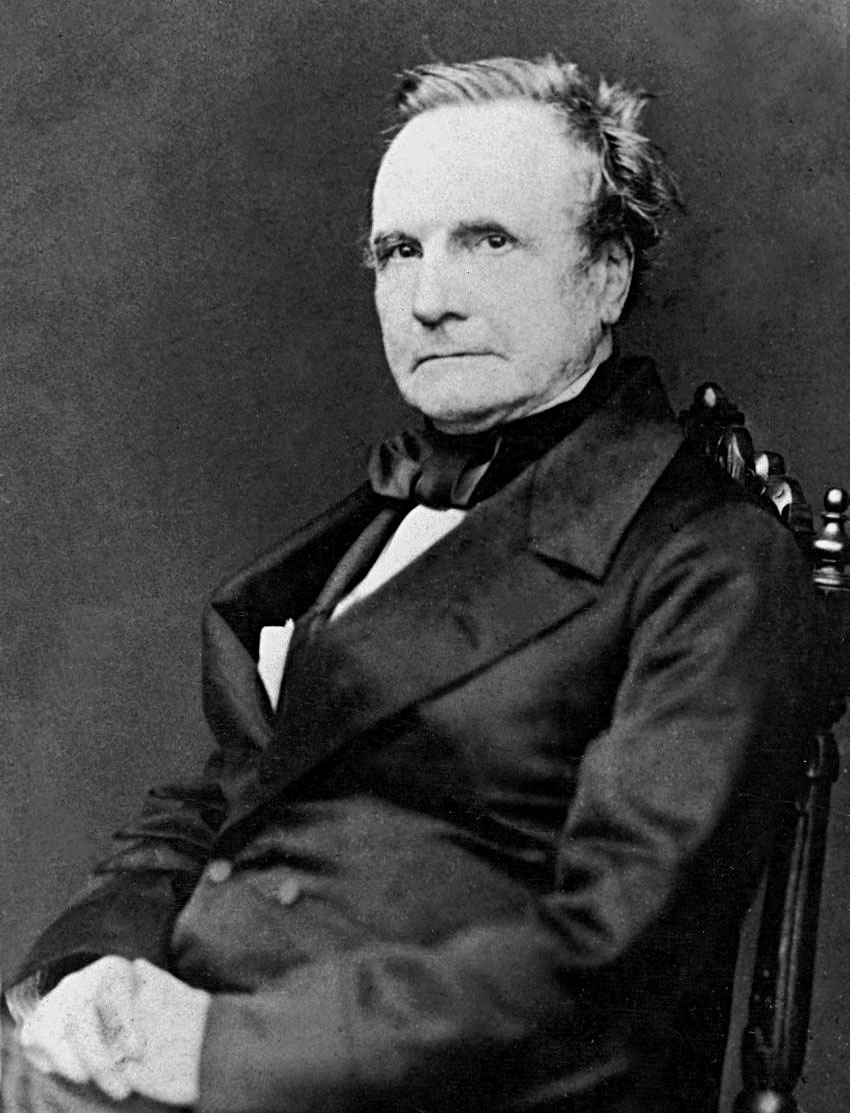
\includegraphics[height=1in]{background/pix/babbage.jpg} \\
  \protect\label{fig:babbage}\protect\href{https://en.wikipedia.org/wiki/Charles_Babbage}{Charles Babbage（查尔斯·巴贝奇），1791--1871} % wikipedia
  \protect\end{tabular}
  \protect\hspace{3em}
  \protect\begin{tabular}[t]{c}
  \protect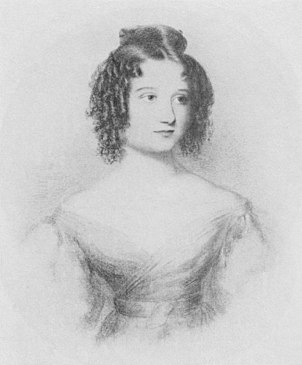
\includegraphics[height=1in]{background/pix/adabyron.jpg} \\
  \protect\label{fig:adabyron}\protect\href{https://en.wikipedia.org/wiki/Ada_Lovelace}{Ada Lovelace（阿达·洛夫莱斯），1815--1852} %
  \protect\end{tabular}
  \protect\end{center}


  然而，这台机器从未完成，因为
  Babbage 又有了制造一台可编程设备的想法，而这诱惑力太大了。\index{programmer!first}
  Lovelace 为一台设想的新机器——分析机——贡献了大量笔记，并因此闻名，被视为第一位程序员。}
典型的例子是编织。\index{weaving}


\begin{center}
  % http://commons.wikimedia.org/wiki/File:Loomwork.jpg
  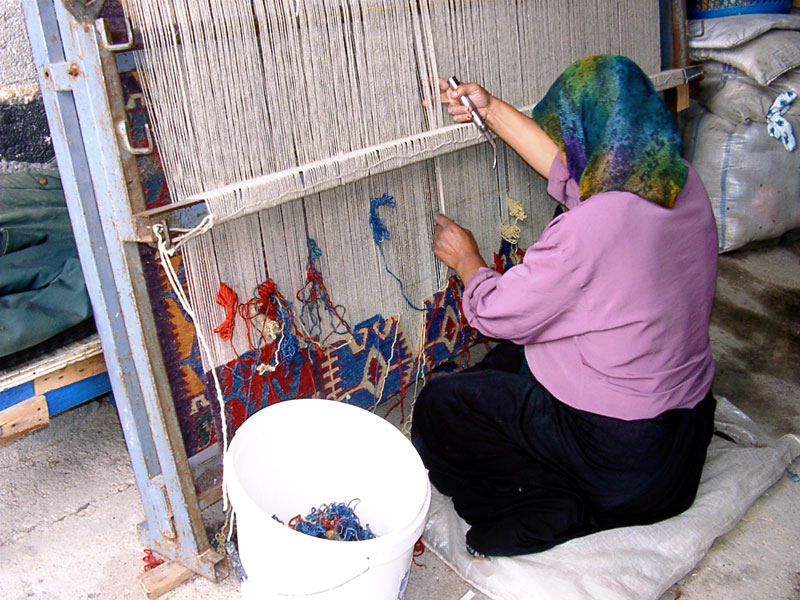
\includegraphics[width=.33\textwidth]{background/pix/loom.jpg}
  \hspace*{2em}
  % http://commons.wikimedia.org/wiki/File:Deutsches_Technikmuseum_Berlin_February_2008_0013.JPG
  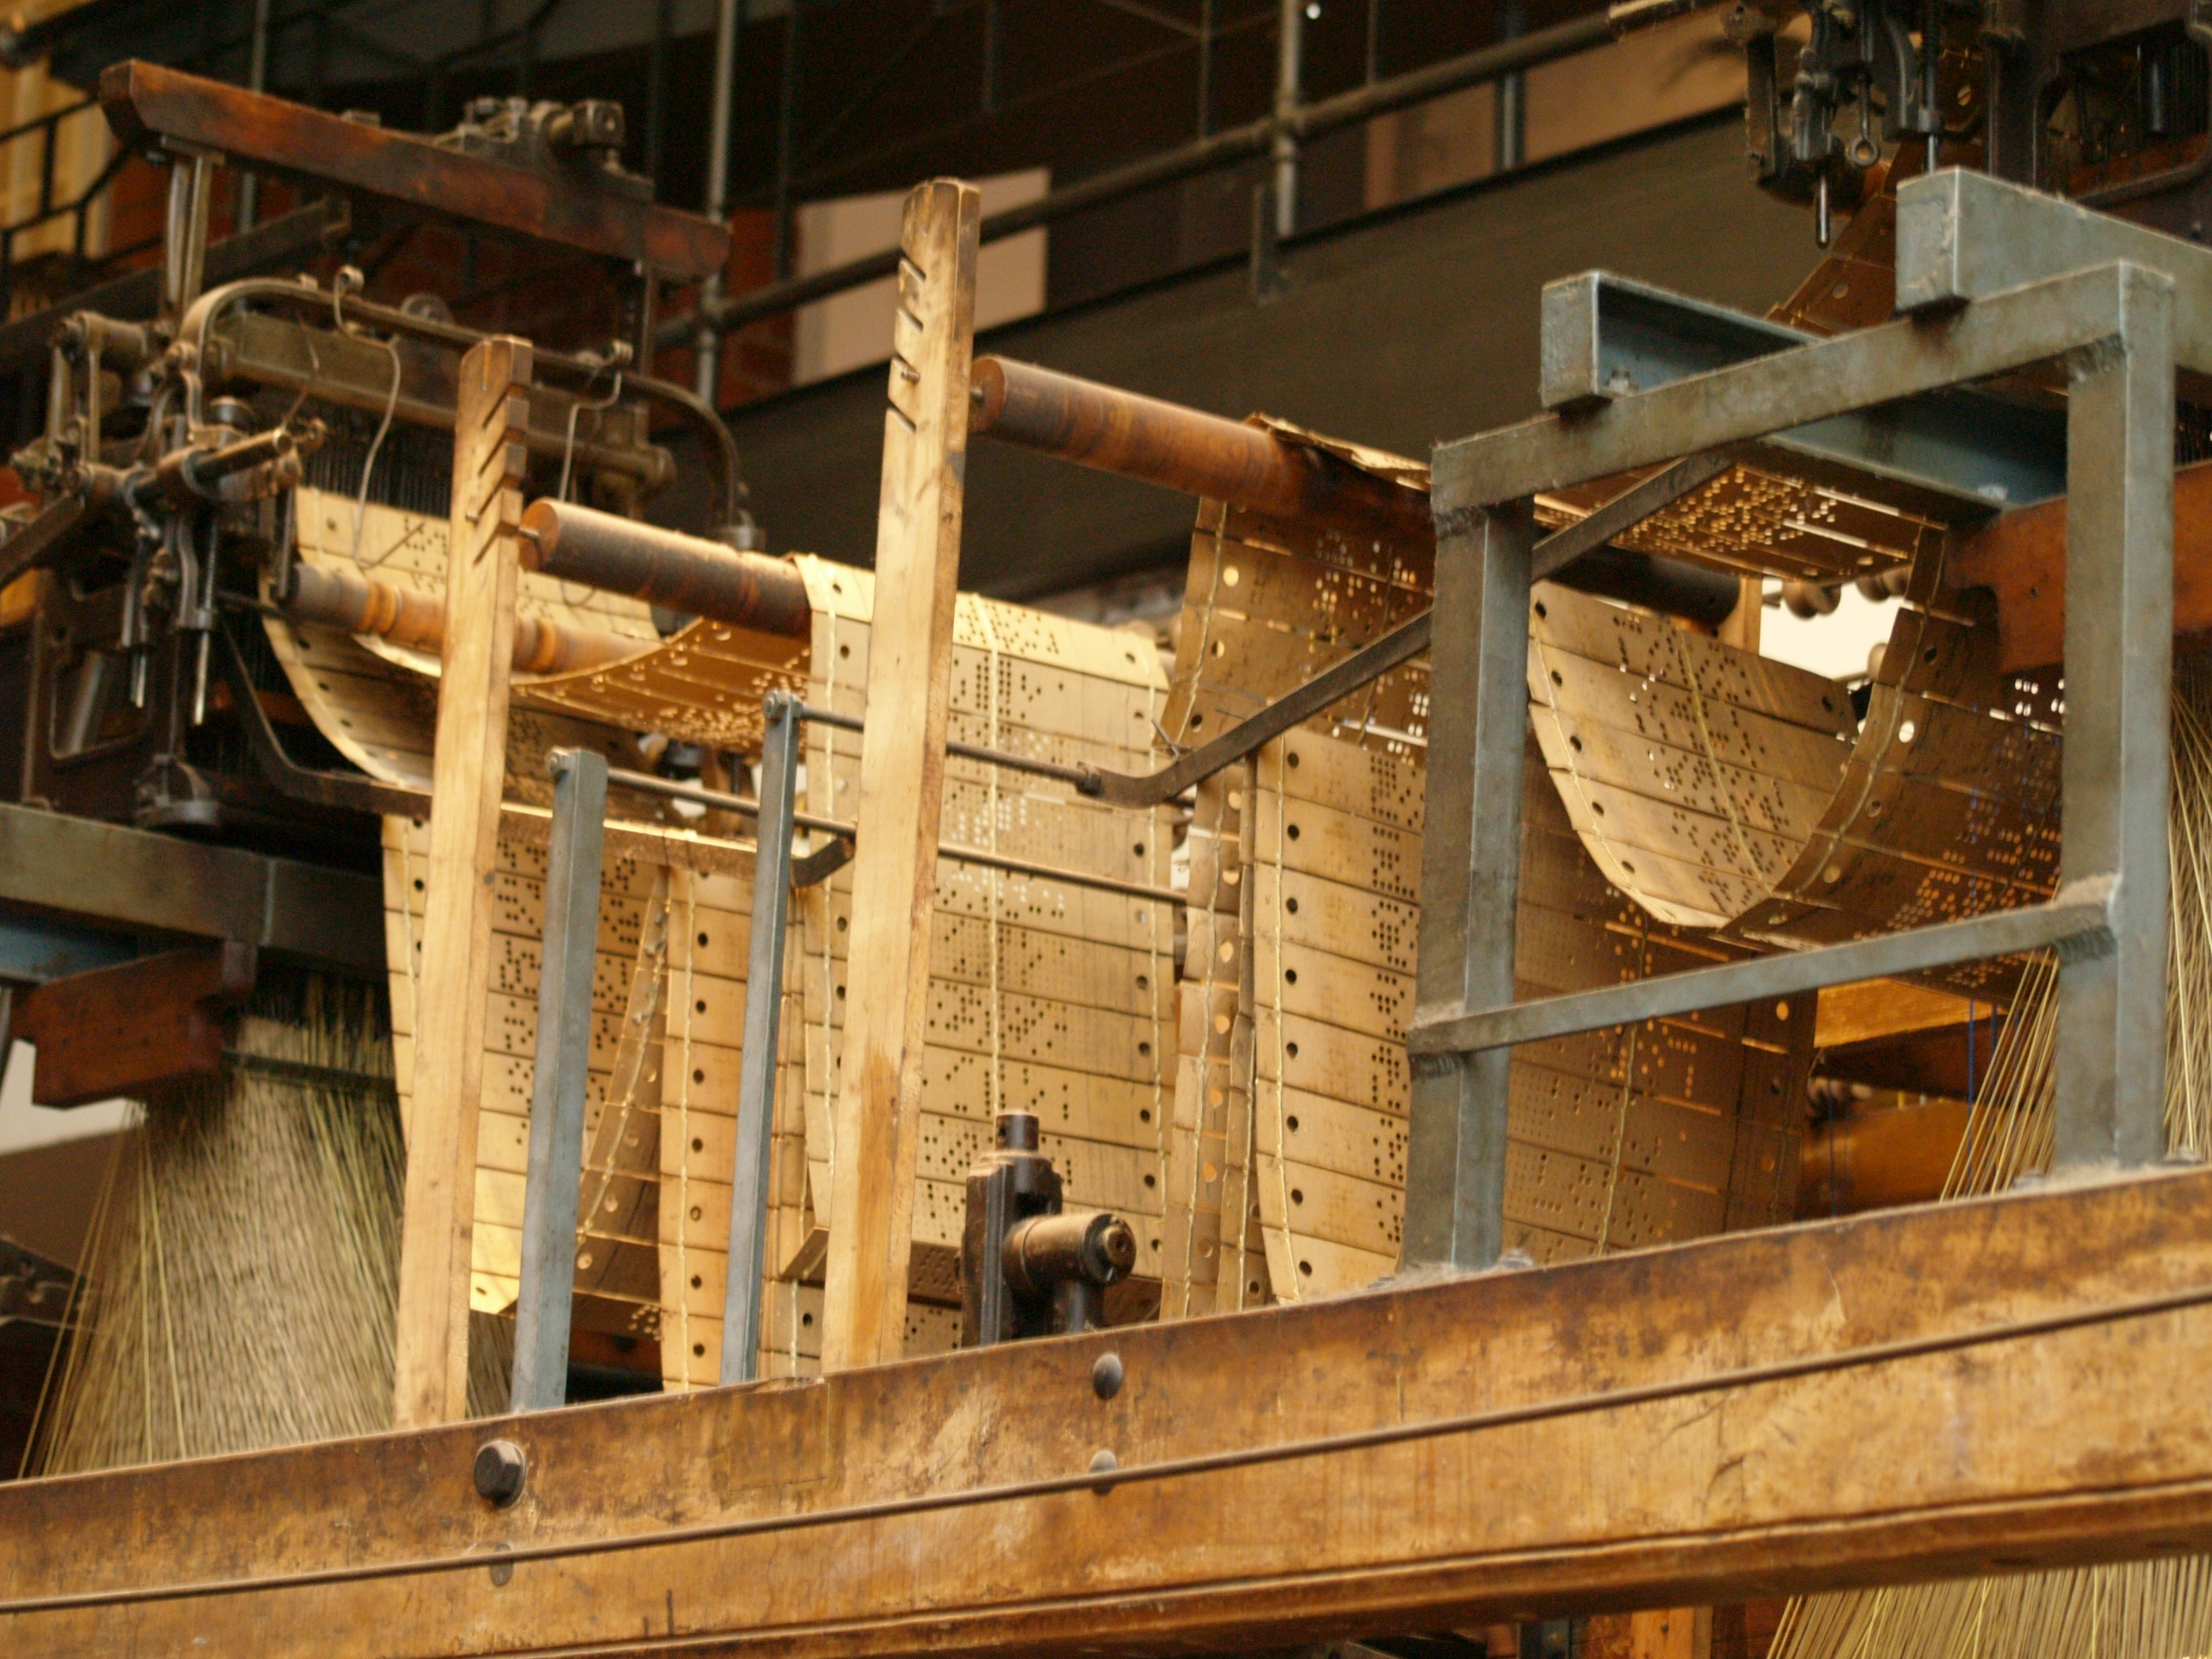
\includegraphics[width=.33\textwidth]{background/pix/jaquardpunchedcards.jpg}
\end{center}


手工织布，如左侧那位织机操作员正在做的，既复杂又缓慢。
我们可以造一台机器来复制她的图案。
但如果我们想要一个不同的图案呢？是否需要另一台机器？
1801年，
\href{https://en.wikipedia.org/wiki/Jacquard_weaving}{J~Jacquard（约瑟夫·玛丽·雅卡尔）}
制造了如右图所示的织布机，\citetext{由卡片控制}{%
  它通过钩子进行编织，钩子提起或放下的位置由卡片上的孔洞决定}。
要获得不同的图案并不需要一台新的织布机，只需要更换一套卡片组即可。

%<*discussion:UniversalTM>
Turing 为计算机引入了与此类似的机制。\index{Turing, Alan}
他构造了一台 Turing 机~$\UTM$，可以向它输入一条纸带，该纸带包含对某台 Turing 机~$\mathcal{M}$ 的描述以及该机器的输入。
然后，$\UTM$ 将表现出与 $\mathcal{M}$ 相同的输入-输出行为。
如果~$\mathcal{M}$
在该输入上停机，那么 $\UTM$ 也将停机并给出相同的输出；
而如果 $\mathcal{M}$ 在该输入上不停机，
那么 $\UTM$ 也不会停机。

只需这一台单独的机器，就能让它表现出任何想要的可计算行为。
因此，我们不需要无穷多台不同的机器，只用 $\UTM$ 就够了。
% This was what we meant by
% saying that a good first take on Turing machines is that they
% are more like a modern computer program than a modern computer\Dash
% on a modern computer, to change behavior we don't change
% the hardware.
%</discussion:UniversalTM>

\margingraphic[l]{0.2\textwidth}{background/pix/snake.png}{\label{fig:ouroboros}\href{https://commons.wikimedia.org/w/index.php?curid=36915535}{衔尾蛇，一条吞食自己尾巴的蛇}}\index{ouroboros}
在陈述 Turing 定理之前，我们先来回答一个经常被问到的问题。
机器~$\UTM$ 似乎引出了一个鸡与蛋的问题：~我们怎么能把一台 Turing 机作为输入给另一台 Turing 机呢？
特别是，既然 $\UTM$ 本身也是一台 Turing 机，
该定理似乎允许将它自身作为输入提供给它自身\Dash 将一台机器喂给它自己，会不会导致无限回归？

\label{page:RepresentingTM}
我们运行 Turing 机，是在纸带上装载好符号，然后按下 \texttt{Start}。
所以我们并不是把机器喂给机器；我们喂给它们的是符号，即事物的表示。
确实，我们可以喂给 $\UTM$ 一个关于它自身的描述，比如一对数 $e,x$，
其中~$e$ 是 $\UTM$ 的索引号（因此在计算上等价于那台机器的源代码），而 $x$ 是输入。
即便如此，宇宙也不会崩溃\Dash
我们完全可以用文本编辑器编辑它自己的源代码，或者让编译器生成它自己的可执行文件。
同理，我们也可以把 $\UTM$ 自己的索引号喂给它。
这样做会引发许多有趣的事情，但首先可以肯定，不存在内在的不可能性。

%<*th:UniversalTM>


\begin{theorem}[Turing, 1936] \label{th:UTM}
存在一台 Turing 机，当输入 $e$ 和 $x$ 时，其输出行为与 $\TM_e$ 在输入 $x$ 上的行为\citetext{相同}{%
  一个技术细节：Turing 机有纸带字母表。
  所以一台通用机的输入或输出只能涉及它被定义为可使用的符号。
  如果另一台机器有不同的纸带字母表，那么通用机该如何模拟它呢？
  和通常一样，我们通过设定让通用机处理另一台机器字母表的表示。
  这类似于日常计算机用二进制来表示十进制数。}。
\end{theorem}


%</th:UniversalTM>

\margingraphicnomag*{0.2\textwidth}{\asydir hp/hp14.pdf}
这就是一台\definend{通用 Turing 机}。\footnote{%
  我们也可以定义一台通用 Turing 机，让它接受单个数 $\cantor(e,x)$ 作为输入。}
\index{Universal Turing machine}\index{Turing machine!universal}%
% We denote such a machine with~$\UTM$.
% Universal machines
% change hardware behavior in software.
% \citetext{This is what a computer's operating
% system does}{%
% }.
此图\footnote{%
  这是一张
\ifbool{MakingPaperCopy}{%
  流程图
}{%
  \citetext{流程图}{%
    流程图被广泛用于勾勒算法；这里有一张来自 XKCD 的图。
    \protect

\begin{center}
    \protect\small
    \protect\begin{tabular}{c}
      \protect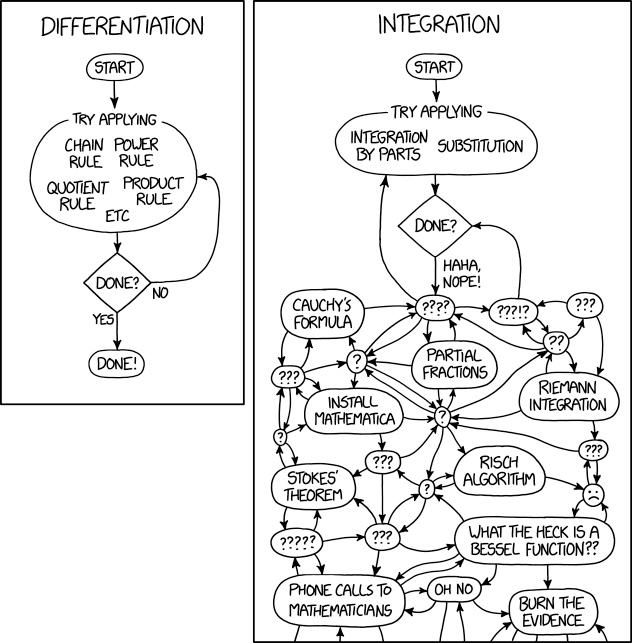
\includegraphics[width=0.25\textwidth]{background/pix/xkcdcalc.png} \\
      \protect\label{fig:xkcdcalc}\protect\href{https://xkcd.com/2117/}{Courtesy xkcd} % wikipedia
    \protect\end{tabular}
    \protect\end{center}

（另参见~\protect\url{http://archive.computerhistory.org/resources/text/Remington_Rand/Univac.Flowmatic.1957.102646140.pdf}）。},
}
  它给出了一个例程的高层示意图。
  我们使用了三种方框。
  圆角方框用于 \protect\texttt{Start} 和
  \protect\texttt{End}。
  矩形方框用于普通的数据操作。
  在后面的图表中我们还会看到菱形方框，
  用于决策，即 \protect\texttt{if} 语句。}\index{flow chart}
勾勒了这样一台机器的行为。

在论证通用机存在之前，我们首先注意到，
通用机器在日常计算中其实很常见。
一方面，
我们可以将此流程图与计算机操作系统的行为进行对比。
操作系统接收一个要运行的程序以及要输入给该程序的数据。
我们可以将程序视作 $\TM_e$，
而将数据视作可解释为数字~$x$ 的比特串。
% The operating system's job is to load the program and feed it the input.
%
操作系统会安排底层硬件表现得如同处理输入~$x$ 的机器~$e$ 一样。
简而言之，与操作系统类似，通用 Turing 机
通过软件改变其行为，
而无需重新插接线。

另一种类似于通用机器的日常计算体验是语言解释器。
下面是与 Racket 解释器的一个交互示例。
在第一个提示符下，我们输入一个例程，它接收
\codeinline!x! 并返回前 \codeinline!x!~个数的和。
在第二个提示符下，我们指定该例程的输入为~$x=4$。
\begin{lstlisting}
$ racket
Welcome to Racket v8.2 [cs].
> (define (triangular x)
      (if (= x 0)
          0
          (+ x (triangular (sub1 x)))))
> (triangular 4)
10
\end{lstlisting}  % $
\label{page:UTM}

计算系统作为通用机器的最直接例子，
是编程语言中的 \codeinline!eval! 语句。\index{eval statement@\texttt{eval} statement}
在下面的第一个提示符下，我们定义了一个例程，它
\citetext{让解释器对输入的表达式求值}{%
  编写一个允许普通用户
  执行任意代码的程序，
  虽然功能强大但并不安全，
  尤其是当这些用户只是从互联网上随意访问时。
  限制用户可以执行的命令，
  即所谓的沙箱化，是谨慎运用这种能力的一部分。
  然而，对我们而言，这些软件工程问题并不相关。}。
在下一个提示符下，我们定义了一个列表（加了引号以防止被求值）。
列表
\codeinline!lambda (i) ...! 描述了一个单输入函数。\footnote{%
  它用“lambda”开始一个函数的定义，因为
  这是 Church 所使用的写法。}
% (in contrast to the definitions
% of the functions \codeinline!triangular! and \codeinline!utm!,
% this function does not have a name and so the definition syntax is
% different).
在第三和第四个提示符下，
解释器对列表中描述的例程求值，
并将其应用于数字~$5$ 和~$0$。
也就是说，就像织布机的打孔卡片一样，
我们可以通过向 \codeinline!utm! 提供任意所需例程的描述，
来改变其行为。
\begin{lstlisting}
> (define (utm s)
      (eval s))
> (define test '(lambda (i) (if (= i 0) 1 0)))
> ((utm test) 5)
0
> ((utm test) 0)
1
\end{lstlisting}

最后，关于该定理的证明，
证明某物存在的最简单方法就是将其构造出来。
我们已经展示过一个本质上就是通用 Turing 机的实例。
在第一章末尾的第~\pageref{extra:TuringMachineSimilator} 页，
我们使用过一个 Turing 机模拟器程序，它
从文件中读取 Turing 机的描述，
然后运行它。
该代码是用 Racket 写的，但
Church 论题断言，我们同样可以写出一台
具有相同行为的 Turing 机。
% (For a Universal Turing machine that meets the criteria, we must not input
% the arbitrary Turing machine from a file, but instead we
% input its index, which we then convert to a Turing machine.
% But we've already argued that we can write a routine to go from
% the index to the Turing machine.)
\index{Universal Turing machine|)}\index{Turing machine!universal|)}

\subsection{一致性}\index{uniformity|(}
考虑这样一个任务：给定一个实数 $r\in\R$，
编写一个程序来输出它的各位数字。
更准确地说，构造一台 Turing 机 $\TM_r$，
使得当输入 $n\in\N$ 时，$\TM_r$ 输出
\citetext{$r$ 的第 $n$ 位小数}{%
  如果数字 $r$ 有不止一种表示法，那么我们可以，
  比如说，输出以 $0$ 结尾的那一种。}
（当~$n=0$ 时，
它输出小数点左边的整数部分）。

我们知道，
并非对所有~$r$ 都能做到这一点，因为虽然
存在不可数多个实数，但 Turing 机只有可数多个。
但究竟是什么阻碍了我们呢？
编程的乐趣之一就在于感觉能让机器做任何事\Dash
为什么不能编写一个程序来输出我们想要的任何数字呢？

确实存在一些实数，可以为它们编写这样的程序，
比如~$11.25$。
\begin{lstlisting}
(define (one-quarter-decimal-places n)
  (cond
      [(= n 0) 11]
      [(= n 1) 2]
      [(= n 2) 5]
      [else 0]))
\end{lstlisting}
对于一个更一般的数，比方说 $r=0.703\ldots$\,，
我们可能会一时想到用穷举法来处理它。
\begin{lstlisting}
(define (r-decimal-place n)
  (cond
    [(= n 0) 0]
    [(= n 1) 7]
    [(= n 2) 0]
    [(= n 3) 3]
    ...
  ))
\end{lstlisting}
但这很可笑。
程序长度有限，因此
不可能包含无限多个分支。

也就是说，由于 \codeinline!if! 语句，
如下程序在输入~$n=7$ 时的行为，
与它在其他输入上的行为互不相关。
\begin{lstlisting}
(define (foo n)
  (if (= n 7)
      42
      (* 2 n)))
\end{lstlisting}
但一个程序只能包含有限多个这样
行为不同的分支。
Turing 机仅有有限条指令这一事实，
对其行为施加了一致性条件。

\begin{example} \label{ex:NineInPi}
以这种方式将“某物可计算”与“它是一致可计算的”这两个观念联系起来，会产生一些令人惊讶的后果。
考虑这样一个问题：编写一个程序，它接收一个数~$n$ 作为输入，然后
判定在 $\pi=3.14159\ldots$ 的十进制展开中，是否
存在 $n$ 个
\citetext{连续的 $9$}{%
  在第 $762$ 位小数处，连续出现了六个 $9$。
  这被称为 Feynman（费曼）点；参见
  \protect\url{https://en.wikipedia.org/wiki/Feynman_point}。
  大多数专家猜想，对于任何~$n$，$\pi$ 的十进制
  展开中都包含连续 $n$ 个 $9$ 的序列，但至今既无人证明也无人推翻这一点。}。

这有两种可能。
要么对于所有~$n$，这样的序列都存在；要么存在某个 $N$，
使得当长度小于~$N$ 时存在连续的 $9$ 序列，
而当 $n\geq N$ 时不存在这样的序列。
因此，这个问题实际上已经解决：以下两个程序之一就是正确的程序
（为说明起见，此处取 $N=1234$）。\label{disc:HP}
\begin{center}
\vspace*{-4ex}
\begin{minipage}[t]{0.4\linewidth}%
\begin{lstlisting}
(define (sequence-of-nines-0 n)
  1)
\end{lstlisting}%
\end{minipage}%
\hspace*{2em}
\begin{minipage}[t]{0.4\linewidth}%
\begin{lstlisting}
(define (sequence-of-nines-1 n)
  (if (< n 1234)
      1
      0))
\end{lstlisting}%
\end{minipage}%
\vspace*{-2ex}
\end{center}

这个论证的一个惊人之处在于，这两个例程似乎与 $\pi$ 并没有多大关系。
同样惊人且或许令人不安的是，我们在没有展示具体解法的情况下，就证明了该问题是可解的。
也就是说，
\citetext{“证明这个函数是可计算的”与“拥有计算它的算法”是两回事}{%
  这有点类似于
  Schr\"odinger（薛定谔）的猫悖论
  (参见 \protect\url{https://en.wikipedia.org/wiki/Schr\%C3\%B6dinger's_cat})，
  因为看起来两者中总有一个是对的，
  但我们就是不知道是哪一个。
  }
\begin{equation*}
  f(n)=
  \begin{cases}
    1 &\case{if $\pi$ has $n$ consecutive nines}  \\
    0 &\case{otherwise}
  \end{cases}
\end{equation*}
这表明，
\citetext{“如果你能为某个东西编写程序，那它就是可计算的”这种说法}{引自 \autocite{SE:JohnL}：
  “我相信大多数人第一次遇到这种证明/结论时，都会感到有些困惑。
  % Or at least myself.
  % The essential point is
  % we do not have to identify/construct/bind to one
  % algorithm that decides [it].
  \ldots{}
  我们并不需要完全理解[那个问题]是什么。
  我们只需要知道，存在一个算法能够判定[它]，无论[答案]最终是什么。
  这偏离了……你可能在接触计算理论之前就有的……那种朴素的可判定性观念。”}
作为一种初步理解或许有用，但至少
遗漏了一些重要的微妙之处。

相比之下，假设我们有一个例程 \codeinline{pi_decimals}
它接收输入~$i\in\N$ 并输出
\citetext{$\pi$ 的第 $i$ 位小数}{%
  如前所述，有些实数有两种十进制
  表示，一种以 $0$ 结尾，一种以 $9$ 结尾。
  但所有这样的数都是有理数（正如“以 $0$ 结尾”所暗示的），
  而 $\pi$ 不是有理数，所以 $\pi$ 不属于这类数。}。
利用它，我们可以编写一个程序，接收输入~$n$，然后
遍历 $\pi$ 的各位数字，
查找连续的 $n$ 个 $9$。
这种方法的好处是，它不仅给出了答案是否存在的结论，还实际构造出了答案。
这种方法也具有“一致性”，因为我们可以
修改它以使用其他例程（如 \codeinline{e_decimals}），
从而在其他数字中寻找连续的 $9$ 串。
然而，这种方法也有一个缺点：如果存在某个 $N$，
使得对于 $n\geq N$，$\pi$ 的十进制展开中都不存在连续 $n$ 个 $9$，
那么这个程序将
无休止地搜索下去，永远无法发现这一情况。
\end{example}


\index{uniformity|)}

\subsection{参数化}\index{parametrization|(}
通用性意味着，存在一台 Turing 机，它
接收输入 $e$ 和~$x$，并返回与在输入~$x$ 上运行 $\TM_e$ 所得相同的值，
包括当 $\TM_e$ 在该输入上不停机时，它也不停机。
也就是说，存在一个可计算
函数 $\map{\phi}{\N^2}{\N}$，使得
若 $\TMfcn_e(x)\converges$ 则 $\phi(e,x)=\TMfcn_e(x)$，若 $\TMfcn_e(x)\diverges$ 则 $\phi(e,x)\diverges$。

在这里，参数~$e$ 从函数的自变量转变为索引，
从而使得 $\phi(e,x)$ 变成了 $\TMfcn_e(x)$。
我们现在将其推广。
从一个接收两个输入的程序开始，
例如下面这个。
\begin{lstlisting}
(define (P x y)
  (+ x y))
\end{lstlisting}
冻结第一个自变量，
结果得到一个单输入程序。
这里，我们先将 $x$ 冻结为~$7$，然后冻结为 $8$。


\begin{center}
\vspace*{-4ex}
\begin{minipage}[t]{0.4\linewidth}%
\begin{lstlisting}
(define (P_7 y)
  (P 7 y))
\end{lstlisting}
\end{minipage}%
\hspace*{2em}
\begin{minipage}[t]{0.4\linewidth}%
\begin{lstlisting}
(define (P_8 y)
  (P 8 y))
\end{lstlisting}
\end{minipage}%
\vspace*{-2ex}
\end{center}

这称为\citetext{\definend{部分应用（partial application）}}{%
  参见 \autocite{wiki:PartialApplication}。}，
因为我们没有冻结所有的输入变量。
相反，我们对
\citetext{\definend{变量~$x$ 进行参数化}}{%
  参数（parameter）是在同一种形式的方程中变化的常数。
  例如，研究二次函数的人可能会考虑方程族 $y=ax^2$；这里 $a$ 就是一个参数。
  所以参数是一种固定的变量。
  （令人难忘的是 A~Perlis 的一句警句，
  “一个人的常量是另一个人的变量。”
  \autocite{Perlis}）
}\index{parametrizing}\index{parameter}
，从而得到一族程序
\codeinline!P_0!、\codeinline!P_1! 等等。

显然，这一族程序与起始程序是相关的。
记上述起始程序~\codeinline{P} 所计算的函数为 $\psi(x,y)=x+y$，
部分应用便给出了如下的函数族：
$\psi_0(y)=y$、$\psi_1(y)=1+y$、$\psi_2(y)=2+y$、\ldots\sentencespace
一般而言，下面的结果表明，
从一个起始 Turing 机（或可计算函数）的索引以及被冻结的值，
我们可以计算出这一族成员的索引。

%<*th:smn>


\begin{theorem}[\smn{} 定理，或称参数定理] \label{th:smn}
\index{Parameter theorem}\index{s-m-n theorem@$s$-$m$-$n$ theorem}
对任意 $m,n\in\N$，存在一个可计算的全函数 $\map{s_{m,n}}{\N^{1+m}}{\N}$
使得对任意 $m+n$ 元函数
$\TMfcn_e(x_0,\ldots\, x_{m-1},x_m,\ldots\, x_{m+n-1})$，
将前 $m$ 个变量冻结于 $a_0,\ldots\, a_{m-1}\in\N$
便得到 $n$ 元可计算函数
$\TMfcn_{s(e,a_0,\ldots a_{m-1})}(x_m,\ldots\, x_{m+n-1})$。% \footnotemark[1]
\end{theorem}


% \footnotetext[1]{%
%   This result is stated in terms of functions, not machines, because
%   the machines need not be the same.
%   That is, they may be unequal as sets of four-tuples.
%   But they will have the same input-output behavior, which means
%   the same function.}
%</th:smn>
% The function $\TMfcn_e(x_0,\ldots x_{m-1},x_m,\ldots x_{m+n-1})$ could be
% partial, that is, it could be that the Turing machine
% $\TM_e$ fails to halt on some inputs $x_0,\ldots x_{m-1},x_m,\ldots x_{m+n-1}$.

\begin{proof}
%<*pf:smni>
我们将构造函数~$s$ 来满足三个
要求：~\citetext{它必须是有效的}{%
  事实上，仔细分析表明它是原始递归的。}；
它必须以索引~$e$ 和一个 $m$ 元组 $a_0,\ldots\, a_{m-1}$ 作为输入；
并且它必须输出一台机器~$\hat{\TM}$ 的索引，使得该机器
在给定输入 $x_m,\ldots\, x_{m+n-1}$ 时，
将返回值 $\TMfcn_e(a_0,\ldots\, a_{m-1},x_m,\ldots\, x_{m+n-1})$，
若该函数发散则不停机。

其思想是：计算~$s$ 的机器将构建~$\hat{\TM}$ 的指令集。
我们能从指令集有效地得出索引，由此即可完成证明。
%</pf:smni>

%<*pf:smnii>
下方左侧是计算函数~$s$ 的机器的流程图。
在其第三个方框中，它生成了右侧简图所示的四元组指令集
$\hat{\TM}$。
左边的机器需要 $a_0,\ldots\, a_{m-1}$ 用于
右侧流程图的第二、三、四框，
还需要 $e$ 用于 $\hat{\TM}$ 的第五框。
%</pf:smnii>
（我们通常尽量避免纠缠于 Turing 机输入输出表示的细节，
但为了尽可能清晰，在右侧的流程图中，我们假设其输入为一元表示，
输入之间用空白符分隔，且机器启动时读写头位于输入最左边的
\str{1} 下方。）
%<*pf:smniii>
\begin{center}
  \vcenteredhbox{\includegraphics{\asydir flowcharts/flowcharts00.pdf}}
  \hspace{3em}
  \vcenteredhbox{\includegraphics{\asydir flowcharts/flowcharts01.pdf}}
\end{center}

最后，注意左边的例程并不运行右边的例程。
相反，它返回实现右侧流程图的 Turing 机 $\hat{\TM}$ 的索引。
它可以在不知道右侧例程是否会停机的情况下生成右侧流程图的源代码，
并由此源代码计算出索引。
因此，由左侧流程图计算的函数~$s$ 是全函数。
%</pf:smniii>
\end{proof}

在记号 $s_{m,n}$ 中，
下标~$m$ 是被冻结的输入个数，
而下标~$n$ 是剩余的自由输入个数。
这些下标可能略显繁琐，我们通常省略它们。

\smn{} 定理的关键点在于它给出的不仅是一个可计算函数，更是一族相关的函数。

\begin{example}
考虑由该流程图描述的双输入例程。
\begin{equation*}
  \vcenteredhbox{\includegraphics{\asydir flowcharts/flowcharts1007.pdf}}
  \tag{$*$}
\end{equation*}
由 Church 论题，存在一台 Turing 机与该草图匹配。
% computing the function $\psi(x,y)=x\cdot y$.
记其索引为~$e_0$。
（下标 ‘0’ 意在强调这个索引是固定的，而非变量；它是某一特定 Turing 机的编号。）

下方左侧是机器 $\TM_{s(e_0,0)}$ 的流程图，它将~$x$ 的值固定为~$0$，从而计算函数 $\TMfcn_{s(e_0,0)}(y)=0$。
例如，$\TMfcn_{s(e_0,0)}(5)=0$。
类似地，另外两个是概括 $\TM_{s(e_0,1)}$ 和~$\TM_{s(e_0,2)}$ 的流程图，
% freezing the value of $x$ at $1$ and~$2$ and therefore
它们计算函数 $\TMfcn_{s(e_0,1)}(y)=y$ 和 $\TMfcn_{s(e_0,2)}(y)=2y$。
\begin{center}
  \vcenteredhbox{\includegraphics{\asydir flowcharts/flowcharts1008.pdf}}
  \hspace{2em}
  \vcenteredhbox{\includegraphics{\asydir flowcharts/flowcharts1009.pdf}}
  \hspace{2em}
  \vcenteredhbox{\includegraphics{\asydir flowcharts/flowcharts1010.pdf}}
  \hspace{2em}\ldots
\end{center}
以下是一般的家族成员，$\TM_{s(e_0,x)}$。
\begin{equation*}
  \vcenteredhbox{\includegraphics{\asydir flowcharts/flowcharts1011.pdf}}
  \tag{$**$}
\end{equation*}
将 ($**$) 与~($*$) 对比。
不同之处在于，($**$) 中的机器并不读入~$x$；相反，若将它们视为程序而非 Turing 机，则 $x$ 被硬编码在源代码的体部中。
\end{example}

该示例展示了 \smn{} 定理如何使我们从单个可计算函数 $\TMfcn_{e_0}$ 得到函数序列
$\TMfcn_{s(e_0,x)}$。
这是一个相关的函数族，
\citetext{它是由~$x$ 参数化的}{%
  如果我们从一个双输入函数
  $\map{\TMfcn_{e_0}(x,y)}{\N^2}{\N}$ 开始，那么对于每个~$x$，\smn{}
  定理实际上产生了一个单输入函数 $\map{\TMfcn_{s(e_0,x)}}{\N}{\N}$。
  也就是说，将 $\N$、$\N$ 和 $\N$ 分别替换为 $A$、$B$ 和 $C$，
  它就把从 $A\times B$ 到~$C$ 的二元映射集合，变换为从 $A$ 到~$D$ 的映射集合中的一个成员，其中 $D$
  是从 $B$ 到~$C$ 的映射集合。
  在某些语境下，例如函数式编程中，这被称为
  \definend{柯里化（currying）}.\index{currying}
}，因为 $e_0$ 是固定的。

换句话说，这个函数族是一致可计算的\Dash 那个单一的可计算函数~$s$（更精确地说是 $s_{1,1}$）从索引~$e_0$ 和参数值~$x$ 出发，映射到 ($**$) 中结果的索引。
所以 \smn{} 定理是关于一致性的。
\index{parametrization|)}

% ..............................................................
\begin{exercises}
\recommended


\begin{exercise}
\begin{credit}
  始于\href{https://cs.stackexchange.com/questions/69197/difference-between-turing-machine-and-universal-turing-machine}{Stack Exchange}
\end{credit}
你的学习小组里有人问：
“通用 Turing 机能做哪些普通 Turing 机做不到的事？”
帮他们理解一下。
\begin{answer}\verified
  通用 Turing 机本身也是一台普通的 Turing 机，因为它只是列表 $\TM_0$、$\TM_1$、\ldots\sentencespace 中的另一台而已。
  或许你的朋友想问的是：“通用 Turing 机能做哪些非通用的 Turing 机做不了的事？”
  每台 Turing 机都执行一项任务。
  有些机器接受单个输入然后将其翻倍，
  有些则将其输入解释为两个数字然后相加。
  通用 Turing 机期待两个输入，$e$ 和~$x$，
  而它的输出与机器 $\TM_e$ 在输入~$x$ 上的输出相同，
  若那台机器不停机，它也不停机。
  它的通用性在于，任何能被机械地产生的输入-输出行为，都可以由这一台设备产生。
\end{answer}
\end{exercise}

\begin{exercise}
是否有人曾建造出通用 Turing 机，
或与之等效的设备？抑或它仅仅停留在理论层面？
\begin{answer}\verified
  每一台通用计算机，包括任何标准的笔记本电脑或手机，
  本质上都是一台通用 Turing 机。

  \textit{注：}
  有些观察者反对“通用计算机本质上是 Turing 机”这一论断，
  理由是笔记本电脑并不具有无限多的内存。
  确实如此。
  但同样不可否认的是，这样的机器可以连接到外部存储器——
  也许是云存储，也许是允许它在纸带上做标记的设备——
  从而它并不受限于内置的 RAM。

  有人还会继续反驳说，物理宇宙中只有数量有限的基本粒子可以用来构成比特，
  因此内存终究不是无限的。
  这或许是真的\Dash 它似乎与当前的物理学相符，
  尽管我们也可以回击说，在大爆炸演变为大挤压（或未来无论发生什么）之前，
  我们根本没有足够的时间去耗尽现有的所有比特。

  然而，在关于 Church 论题的章节中我们曾指出，
  Turing 机的定义将直观上的可计算概念精确化了。
  也就是说，“Turing 机”的关键在于，
  它是思考算法的正确模型；它是一种数学理想化。
  笔记本电脑则是同一概念的物理实例化。

  确实，从某种意义上说它们不能是同一事物，因为那将是类型错误\Dash
  一个的类型是“数学对象”，而另一个的类型是“物理对象”。
  同理，木工用的丁字尺是直角这一数学理想的实例化。
  以无人能制造出精确到小数位数超过宇宙中基本粒子数的完美直角为由，
  断言丁字尺是不合法的，这似乎忘记了我们为何觉得思考模型是有用的。
  实例化的本质即是理想化。
\end{answer}
\end{exercise}

\begin{exercise}
一台通用 Turing 机能够模拟另一台通用 Turing 机吗？
甚至，它能模拟它自己吗？
\begin{answer}\verified
  能。
  如果 $\TM_{e_0}$ 和 $\TM_{e_1}$ 是通用 Turing 机，
  那么给第一台输入 $e_1$ 和 $x$，
  将产生与第二台完全相同的输入输出行为。
  同样地，给 $\TM_{e_0}$ 输入 $e_0$ 和 $x$，
  其行为将与它自身完全一致。
\end{answer}
\end{exercise}

\recommended

\begin{exercise}
\begin{credit}
  来自
  \href{https://cs.stackexchange.com/q/41854/67754}{Stack Exchange 上的一个问题}.
\end{credit}
你们班上有同学说：
“我搞不懂通用 Turing 机。
一台机器怎么能模拟拥有更多状态的另一台机器呢？”
请纠正他们的错误认识。
\begin{answer}\verified
  通用机并不是使用自己的状态去模拟另一台机器的状态。
  相反，它拥有这些状态的编码，并对这些编码进行操作。
  简而言之，它通过软件进行模拟，因此通用机自身的状态数量与此无关。
\end{answer}
\end{exercise}

\begin{exercise}
是否存在不止一台通用 Turing 机？
\begin{answer}\verified
是的，根据~\zcref{lem:EveryCompFcnHasInfManyIndices}，
每个可计算函数都有无穷多个索引。
因此，如果 $\TM_e$ 是通用的，那么其关联函数~$\TMfcn_e$
就有无穷多个互不相同的索引：
$\TMfcn_e=\TMfcn_{e_0}=\TMfcn_{e_1}=\cdots\,$。
这些机器
$\TM_{e_0}$, $\TM_{e_1}$, \ldots{} 各不相同，但它们具有相同的
输入输出行为，因此都是通用的。
\end{answer}
\end{exercise}

% \begin{exercise}
% What happens if we feed a Universal Turing machine to itself?
% For instance, where the index~$e_0$ is such that
% $\TMfcn_{e_0}(e,x)=\TMfcn_e(x)$ for all~$x$,
% what is the value of
% $\TMfcn_{e_0}(e_0,5)$?
% \begin{answer}
% We know that $5$ equals $\cantor(2,0)$, that is, $\pair(5)=\sequence{2,0}$.
% So in $\TMfcn_{e_0}(e_0,5)$ the argument to $\TMfcn_{e_0}$ is the
% value of $\TMfcn_2(0)$.
% So, where $\pair(\TMfcn_2(0))=\sequence{a,b}$, the value of
% $\TMfcn_{e_0}(e_0,5)$ is $\TMfcn_a(b)$.
% \end{answer}
% \end{exercise}

\recommended

\begin{exercise}
考虑函数 $f(x_0,x_1)=3x_0+x_0\cdot x_1$。
\begin{exparts}
\item 将 $x_0$ 冻结为值~$4$。
  得到的一元函数是什么？
\item 将 $x_0$ 冻结为~$5$。
  得到的一元函数是什么？
\item 将 $x_1$ 冻结为~$0$。
  得到的函数是什么？
\end{exparts}
\begin{answer}\verified
我们将 $x_i$ 冻结为值~$a$ 所得的函数记作 $f_{i,a}$。
\begin{exparts}
\item 得到的一元函数是 $f_{0,4}(x_1)=12+4x_1$。
\item 得到的一元函数是 $f_{0,5}(x_1)=15+5x_1$。
\item 得到的一元函数是 $f_{1,0}(x_0)=3x_0$。
\end{exparts}
\end{answer}
\end{exercise}

\begin{exercise}
考虑
$f(x_0,x_1,x_2)=x_0+2x_1+3x_2$。
\begin{exparts}
\item 将 $x_0$ 冻结为值~$1$。
  得到的二元函数是什么？
\item 将 $x_0$ 冻结为 $2$ 会得到什么二元函数？
\item 设 $a$ 为自然数。
  将 $x_0$ 冻结为 $a$ 会得到什么二元函数？
\item 将 $x_0$ 冻结为~$5$，$x_1$ 冻结为~$3$。
  得到的一元函数是什么？
\item 对于 $a,b\in\N$，将 $x_0$ 冻结为~$a$，$x_1$ 冻结为~$b$ 会得到什么一元函数？
\end{exparts}
\begin{answer}\verified
我们用 $\hat{f}$ 来命名各个函数。
\begin{exparts}
\item 得到的二元函数是
  $\hat{f}(x_1,x_2)=1+2x_1+3x_2$。
\item 结果是二元函数
  $\hat{f}(x_1,x_2)=2+2x_1+3x_2$。
\item 这给出
  $\hat{f}(x_1,x_2)=a+2x_1+3x_2$。
\item 这得到一元函数
  $\hat{f}(x_2)=11+3x_2$。
\item 结果是
  $\hat{f}(x_2)=a+2b+3x_2$。
\end{exparts}
\end{answer}
\end{exercise}

\recommended


\begin{exercise}
假设由该流程图描绘的 Turing 机的索引为~$e_0$。
\begin{center}
  \includegraphics{\asydir flowcharts/flowcharts1000.pdf}
\end{center}
\begin{exparts}
\item 描述函数 $\TMfcn_{s_{1,1}(e_0,1)}$。
\item 求 $\TMfcn_{s_{1,1}(e_0,1)}(0)$、
  $\TMfcn_{s_{1,1}(e_0,1)}(1)$ 和~$\TMfcn_{s_{1,1}(e_0,1)}(2)$ 的值。
\item 描述函数 $\TMfcn_{s_{1,1}(e_0,0)}$。
\item 求 $\TMfcn_{s_{1,1}(e_0,0)}(0)$、
  $\TMfcn_{s_{1,1}(e_0,0)}(1)$ 和~$\TMfcn_{s_{1,0}(e_0,0)}(2)$ 的值。
\end{exparts}
\begin{answer}\verified
由机器的流程图，我们得到其关联函数
$\TMfcn_{e_0}(x_0,x_1)=x_0+x_1$。
\begin{exparts}
\item $s_{1,1}$ 的两个下标意味着
  我们将冻结第一个输入，并将第二个保留为变量。
  所以 $\TMfcn_{s_{1,1}(e_0,1)}$ 将是一个一元函数。
  参数 $e_0$ 和~$1$ 表明我们正在处理
  Turing 机~$e_0$（即题目中给出流程图的那台机器），
  且输入被冻结为 $x_0=1$。
  此流程图给出了结果的示意。
  \begin{center}
    \includegraphics{\asydir flowcharts/flowcharts1001.pdf}
  \end{center}
  该函数为 $\TMfcn_{s_{1,1}(e_0,1)}(x_1)=1+x_1$。
\item 其值为 $\TMfcn_{s_{1,1}(e_0,1)}(0)=1$、
  $\TMfcn_{s_{1,1}(e_0,1)}(1)=2$ 和~$\TMfcn_{s_{1,1}(e_0,1)}(2)=3$。
\item 记号 $s_{1,1}(e_0,0)$ 表示我们处理 Turing 机~$e_0$，
  将第一个输入冻结为 $x_0=0$，
  并将第二个输入保留为变量。
  此流程图展示了其大意。
  \begin{center}
    \includegraphics{\asydir flowcharts/flowcharts1002.pdf}
  \end{center}
  该函数为 $\TMfcn_{s_{1,1}(e_0,1)}(x_1)=0+x_1=x_1$。
\item 我们有 $\TMfcn_{s_{1,1}(e_0,0)}(0)=0$、
  $\TMfcn_{s_{1,1}(e_0,0)}(1)=1$ 和~$\TMfcn_{s_{1,1}(e_0,0)}(2)=2$。
\end{exparts}
\end{answer}
\end{exercise}

\begin{exercise}
设由该流程图描绘的 Turing 机的索引为~$e_0$。
\begin{center}
  \includegraphics{\asydir flowcharts/flowcharts1003.pdf}
\end{center}
\begin{exparts}
\item 描述函数 $\TMfcn_{s_{1,2}(e_0,1)}$。
\item 求 $\TMfcn_{s_{1,2}(e_0,1)}(0,1)$、
  $\TMfcn_{s_{1,2}(e_0,1)}(1,0)$ 和~$\TMfcn_{s_{1,2}(e_0,1)}(2,3)$。
\item 描述函数 $\TMfcn_{s_{2,1}(e_0,1,2)}$。
\item 求 $\TMfcn_{s_{2,1}(e_0,1,2)}(0)$、
  $\TMfcn_{s_{2,1}(e_0,1,2)}(1)$ 和~$\TMfcn_{s_{2,1}(e_0,1,2)}(2)$。
\end{exparts}
\begin{answer}\verified
由机器的流程图可知，关联函数为
$\TMfcn_{e_0}(x_0,x_1,x_2)=x_0+x_1\cdot x_2$。
\begin{exparts}
\item 记号 $s_{1,2}(e_0,1)$ 表示
  我们处理 $\TM_{e_0}$，
  将第一个输入冻结为 $x_0=1$，
  并将第二个和第三个输入保留为变量。
  此流程图勾勒了其行为。
  \begin{center}
    \includegraphics{\asydir flowcharts/flowcharts1004.pdf}
  \end{center}
  该函数为 $\TMfcn_{s_{1,2}(e_0,1)}(x_1,x_2)=1+x_1\cdot x_2$。
\item 我们有 $\TMfcn_{s_{1,2}(e_0,1)}(0,1)=1$、
  $\TMfcn_{s_{1,2}(e_0,1)}(1,0)=1$ 和~$\TMfcn_{s_{1,2}(e_0,1)}(2,3)=7$。
\item $s_{2,1}(e_0,1,2)$ 表示我们从 $\TM_{e_0}$ 出发，
  将第一个输入冻结为 $x_0=1$，第二个输入冻结为 $x_1=2$，
  并将第三个输入保留为变量。
  此流程图勾勒了结果。
  \begin{center}
    \includegraphics{\asydir flowcharts/flowcharts1005.pdf}
  \end{center}
  该函数为 $\TMfcn_{s_{2,1}(e_0,1,2)}(x_2)=1+2\cdot x_2$。
\item 其值为 $\TMfcn_{s_{2,1}(e_0,1,2)}(0)=1$、
  $\TMfcn_{s_{2,1}(e_0,1,2)}(1)=3$ 和~$\TMfcn_{s_{2,1}(e_0,1,2)}(2)=5$。
\end{exparts}
\end{answer}
\end{exercise}

\recommended


\begin{exercise}
假设由该流程图描绘的 Turing 机的索引为~$e_0$。
\begin{center}
  \includegraphics{\asydir flowcharts/flowcharts1006.pdf}
\end{center}
\begin{exparts*}
\item 描述 $\TMfcn_{s_{1,1}(e_0,0)}$。
\item 求 $\TMfcn_{s_{1,1}(e_0,0)}(5)$。
\item 描述 $\TMfcn_{s_{1,1}(e_0,1)}$。
\item 求 $\TMfcn_{s_{1,1}(e_0,1)}(5)$。
\item 描述 $\TMfcn_{s_{1,1}(e_0,2)}$。
\item 求 $\TMfcn_{s_{1,1}(e_0,2)}(5)$。
\end{exparts*}
\begin{answer}\verified
由机器的流程图可知，关联函数如下：
\begin{equation*}
  \TMfcn_{e_0}(x_0,x_1)=
  \begin{cases}
    x_1  &\case{if $x_0\leq 1$}  \\
    \,\diverges &\case{otherwise}
  \end{cases}
\end{equation*}
\begin{exparts}
\item $\TMfcn_{s_{1,1}(e_0,0)}(x_1)=x_1$
\item $\TMfcn_{s_{1,1}(e_0,0)}(5)=5$
\item $\TMfcn_{s_{1,1}(e_0,1)}(x_1)=x_1$
\item $\TMfcn_{s_{1,1}(e_0,1)}(5)=5$
\item $\TMfcn_{s_{1,1}(e_0,2)}(x_1)\diverges$
\item $\TMfcn_{s_{1,1}(e_0,2)}(5)\diverges$
\end{exparts}
\end{answer}
\end{exercise}

\recommended

\begin{exercise}
设由该流程图所概略描述的 Turing 机的索引为~$e_0$。
\begin{center}
  \includegraphics{\asydir flowcharts/flowcharts1012.pdf}
\end{center}
我们将描述一个以自变量~$x_0$ 和~$x_1$ 为参数的函数族。
\begin{exparts}
\item 如同在 \smn{} 定理中那样，固定 $x_0=0$ 和~$x_1=3$。
  描述 $\TMfcn_{s(e_0,0,3)}$。
  $\TMfcn_{s(e_0,0,3)}(5)$ 是多少？
\item
  描述 $\TMfcn_{s(e_0,1,3)}$。
  $\TMfcn_{s(e_0,1,3)}(5)$ 是多少？
\item 描述 $\TMfcn_{s(e_0,a,b)}$。
\end{exparts}
\begin{answer}
从该机的流程图可以看出，与之关联的函数为：
\begin{equation*}
  \TMfcn_{e_0}(x_0,x_1,y)=
  \begin{cases}
    x_1\cdot y  &\case{if $x_0$ is even}  \\
    x_1+y       &\case{otherwise}
  \end{cases}
\end{equation*}
\begin{exparts}
\item 此函数 $\TM_{s(e_0,0,3)}$ 有 $x_0=0$，因此 $x_0$ 是偶数。
  \begin{center}
    \includegraphics{\asydir flowcharts/flowcharts1013.pdf}
  \end{center}
  因此该函数是 $\TMfcn_{s(e_0,0,3)}(y)=3y$。
  于是，$\TMfcn_{s(e_0,0,3)}(5)=15$。
\item 此函数有 $x_0=1$，因此 $x_0$ 是奇数。
  此流程图概略描述了 $\TM_{s(e_0,1,3)}$。
  \begin{center}
    \includegraphics{\asydir flowcharts/flowcharts1014.pdf}
  \end{center}
  计算出的函数是 $\TMfcn_{s(e_0,1,3)}(y)=3+y$，
  因而 $\TMfcn_{s(e_0,1,3)}(5)=8$。
\item
  这是概略描述 $\TM_{s(e_0,a,b)}$ 的流程图。
  \begin{center}
    \includegraphics{\asydir flowcharts/flowcharts1015.pdf}
  \end{center}
  此流程图与问题陈述中的流程图之间的区别在于，此处的机器并不读取~$x_0$ 或~$x_1$。
  参数 $a$ 和~$b$ 被硬编码在程序体中。
  这是一个以~$a$ 和~$b$ 为参数的函数族，且利用 \smn{} 函数~$s$，这些函数的索引可以从 $e_0$、$a$ 和~$b$ 一致可计算。
  \begin{equation*}
    \TMfcn_{s(e_0,a,b)}(y)=
    \begin{cases}
      b\cdot y  &\case{if $a$ is even}  \\
      b+y       &\case{otherwise}
    \end{cases}
  \end{equation*}
\end{exparts}
\end{answer}
\end{exercise}

% \recommended
% \begin{exercise}
% \begin{exparts*}
% \item Argue that the function $\map{\psi}{\N^2}{\N}$ given by $\psi(x,y)=3x+y$
%   is computable.
% \item Show that there
%   is a family of computable functions $\psi_n$ parameterized by~$n$ such
%   that $\psi_n(y)=3n+y$.
% \item Argue that $n$ is computable.
% \end{exparts*}
% \begin{answer}\verified
% \begin{exparts}
% \item The function  $\psi(x,y)=3x+y$ is computable by Church's Thesis,
%   as sketched in this flowchart.
%   \begin{center}
%     \includegraphics{\asydir flowcharts/flowcharts1018.pdf}
%   \end{center}
% \item  By the prior item there is a Turing machine that
%   computes the function~$\psi$.
%   Suppose that it is~$\TM_{e_0}$.
%   The \smn{} theorem gives that
%   $\TM_{s_{1,1}(e_0,n)}$ computes the function $y\mapsto 3n+y$.
%   Take $\psi_n=\TMfcn_{s_{1,1}(e_0,n)}$.
% \end{exparts}
% \end{answer}
% \end{exercise}

\recommended


\begin{exercise}
证明存在一个全可计算函数 $\map{g}{\N}{\N}$，
使得 Turing 机 $\TM_{g(n)}$ 计算函数 $y\mapsto y+n^2\!$。
\begin{answer}\verified
  考虑由 $\psi(x,y)=y+x^2\!$ 定义的函数 $\map{\psi}{\N^2}{\N}$。
  它直观上是可计算的，因为它可由该流程图所概略描述的机器计算。
  \begin{center}
    \includegraphics{\asydir flowcharts/flowcharts1016.pdf}
  \end{center}
  依据 Church 论题，存在一台 Turing 机计算它。
  设该机器的索引为~$e_0$，即假设 $\psi(x,y)=\TMfcn_{e_0}(x,y)$。
  根据 \smn{} 定理，存在一个以~$n$ 为参数的可计算函数族 $\TMfcn_{s_{1,1}(e_0,n)}$，
  具有期望的行为 $\TMfcn_{s_{1,1}(e_0,n)}(y)=y+n^2$。
  取 $g(n)$ 为~$s_{1,1}(e_0,n)$（$e_0$ 不是变量，它是上述机器的固定索引）。
\end{answer}
\end{exercise}

\recommended


\begin{exercise}
证明存在一个全可计算函数 $\map{g}{\N^2}{\N}$，
使得 Turing 机 $\TM_{g(m,b)}$ 计算函数 $x\mapsto mx+b$。
\begin{answer}\verified
  考虑函数 $\psi(u,v,x)=ux+v$。
  它直观上是可计算的，如该流程图所概略描述的那样。
  \begin{center}
    \includegraphics{\asydir flowcharts/flowcharts1017.pdf}
  \end{center}
  依据 Church 论题，存在一台 Turing 机计算它。
  设该机器的索引为~$e_0$，即假设 $\psi(u,v,x)=\TMfcn_{e_0}(u,v,x)$。
  \smn{} 定理给出了一个以~$m$ 和~$b$ 为参数的可计算函数族
  $\TMfcn_{s_{2,1}(e_0,m,b)}$，
  具有期望的行为 $\TMfcn_{s_{2,1}(e_0,m,b)}(x)=m\cdot x+b$。
  取 $g(m,b)$ 为 $s_{2,1}(e_0,m,b)$
  （注意：$e_0$ 不是变量，它是该流程图对应的 Turing 机的固定索引）。
\end{answer}
\end{exercise}

\recommended


\begin{exercise}
假设 $e_0$ 满足：$\TMfcn_{e_0}$ 是由一台通用 Turing 机计算的函数，这意味着若输入为 $\cantor(e,x)$，则它返回与 $\TM_e(x)$ 相同的值。
再假设~$e_1$ 满足：对所有~$x\in\N$，$\TMfcn_{e_1}(x)=4x$。
如果可能，求出以下各项的值（如果不可能，则简要说明理由）。
\begin{exparts}
\item $\TMfcn_{e_0}(\cantor(e_1,5))$
\item $\TMfcn_{e_1}(\cantor(e_0,5))$
\item $\TMfcn_{e_0}(\cantor(e_0,\cantor(e_1,5)))$
\end{exparts}
\begin{answer}\verified
\begin{exparts}
\item
  这与 $\TMfcn_{e_1}(5)$ 的结果相同，即它收敛并给出~$20$。
\item
  这将返回 $\cantor(e_0,5)$ 值的~$4$ 倍。
  我们不知道~$e_0$ 的值，所以最多只能得出这些。
\item 由第一项可知，这将返回 $\TMfcn_{e_0}(20)$。
  因为 $\pair(20)=\sequence{5,0}$，所以这是 $\TMfcn_5(0)$ 的值，无论其具体是多少。
\end{exparts}
\end{answer}
\end{exercise}

\begin{exercise}
假设 $e_0$ 满足：$\TMfcn_{e_0}(\cantor(e,x))$
返回的值与 $\TMfcn_e(x)$ 相同（或者在该函数不收敛时也不收敛）。
再假设 $\TMfcn_{e_1}(x)=x+2$，
并且对所有~$x\in\N$ 都有 $\TMfcn_{e_2}(x)=x^2$。
如果可能，求出以下各项的值（如果不可能，请简要说明原因）。
\begin{exparts}
\item $\TMfcn_{e_0}(4)$
\item $\TMfcn_{e_0}(\cantor(e_1,4))$
\item $\TMfcn_{e_0}(\cantor(4,e_1))$
\item $\TMfcn_{e_1}(\cantor(e_0,4))$
% \item $\TMfcn_{e_0}(\cantor{e_0,\cantor{e_2,e_1}})$
\end{exparts}
\begin{answer}\verified
\begin{exparts}
\item 因为 $\pair(4)=\sequence{1,1}$，它返回的值与 $\TMfcn_1(1)$ 相同，无论该值是什么。
\item
  这与 $\TMfcn_{e_1}(4)$ 的结果相同，即 $6$。
\item
  它返回 $\phi_4(e_1)$ 的值，无论该值是什么。
\item 它返回 $2+\cantor(e_0,4)$。
$\cantor(e_0,4)$ 的值依赖于 $e_0$，而我们不知道 $e_0$。
我们最多只能说 $\cantor(e_0,4)=e_0+(e_0+4)(e_0+5)/2$。
\end{exparts}
\end{answer}
\end{exercise}

\begin{exercise}
编写一个能读取文件并返回其首字符的程序。
将该程序应用于它自身的源代码。
\begin{answer}\verified
图 \figureref{fig:RacketReadSource} 中提供了 Racket 代码。
\begin{figure}
  \centering
  \lstinputlisting[firstline=3]{scheme/background/first-char.rkt}
  \caption{返回文件首字符的 Racket 代码。}
  \label{fig:RacketReadSource}
\end{figure}
以下是在其自身源代码上运行的结果。
\begin{lstlisting}
> (first-char "first-char.rkt")
#\#
\end{lstlisting}
\end{answer}
\end{exercise}

\begin{exercise}
编写一个自修改程序。
具体来说，编写一个设置变量 \codeinline{COUNTER} 的程序，要求它在运行时能在源代码中递增该变量，并打印出新值。
\begin{answer}\verified
图 \figureref{fig:RacketSelfModifying} 中提供了 Racket 代码。
\begin{figure}
  \centering
  \lstinputlisting{scheme/background/self-modifying.rkt}
  \caption{自修改的 Racket 代码。}
  \label{fig:RacketSelfModifying}
\end{figure}
以下是在其自身源代码上运行的结果。
\begin{lstlisting}
jim@millstone:~/computing/src/scheme/background$ ./self-modifying.rkt
Counter=11
jim@millstone:~/computing/src/scheme/background$ ls -l self-modifying.rkt
-rw-rw-r-- 1 jim jim 1463 Aug 28 10:17 self-modifying.rkt
jim@millstone:~/computing/src/scheme/background$ chmod u+x self-modifying.rkt
jim@millstone:~/computing/src/scheme/background$ ./self-modifying.rkt
Counter=12
\end{lstlisting}
运行后，源代码的第三行现在变为 \codeinline{(define COUNTER 12)}。
\end{answer}
\end{exercise}


\end{exercises}
\index{universality|)}

%================================================
\section{停机问题}\index{Halting problem@\probname{Halting} problem|(}\index{unsolvability|(}\index{unsolvable problem|(} \label{sec:HaltingProblem}
我们已经证明了存在一些函数是无法机械计算的。
我们给出了一个计数论证：Turing 机有可数多台，但函数有不可数多个，因此有些函数没有对应的机器。
尽管了解这一事实是好的，但能展示一个具体的不可解函数则更有价值。
我们现在就来做这件事。

\subsection{定义} \label{sec:Unsolvability}
要构造这样一个函数，自然的思路是利用 Cantor 定理并将其“可计算化”，把这个证明变成一个具体的构造。

下面是一个示例表格，改编自第~\pageref{ex:DiagonalizationTable}页关于 Cantor 定理的讨论。\index{diagonalization!effectivized}
设想这个表格的行是可计算函数，列是输入。
例如，这个表格列出了 $\phi_2(3)=5$。


\begin{center} \small \label{HPDiagonalizationTable}
  %<*table:CantorThmEffectivization>
  \setlength{\arraycolsep}{0.75\arraycolsep}
  \begin{minipage}{4em}\vspace*{0cm}\tabulartext{函数}\end{minipage}
  \begin{tabular}{r|ccccccc@{\hspace*{1em}$\ldots$}}
    \multicolumn{1}{r}{\ }
    &\multicolumn{7}{c}{\text{\tabulartext{输入}}}  \\
     % \multicolumn{1}{c}{\text{\tabulartext{Function}}}
     \multicolumn{1}{c}{\ }
    &$0$ &$1$ &$2$ &$3$ &$4$ &$5$ &$6$ \\
   \cline{2-8}
   \rule{0em}{2.15ex}% bit more vertical room
   $\phi_0$  &$3$  &$1$  &$2$  &$7$  &$7$  &$0$  &$4$  \\
   $\phi_1$  &$0$  &$5$  &$0$  &$0$  &$0$  &$0$  &$0$  \\
   $\phi_2$  &$1$  &$4$  &$1$  &$5$  &$9$  &$2$  &$6$  \\
   $\phi_3$  &$9$  &$1$  &$9$  &$1$  &$9$  &$1$  &$9$  \\
   $\phi_4$  &$1$  &$0$  &$1$  &$0$  &$0$  &$1$  &$0$  \\
   $\phi_5$  &$6$  &$2$  &$5$  &$5$  &$4$  &$1$  &$8$  \\
   \multicolumn{1}{r}{$\vdotswithin{0}$}
    &\multicolumn{6}{c}{$\vdotswithin{0}$}
  \end{tabular}
  %</table:CantorThmEffectivization>
  \hspace*{2em plus 0.75fil}
  \vcenteredhbox{\includegraphics{\asydir hp/hp02.pdf}}
\end{center}


%<*discussion:HP>
对角化意味着考虑右边的机器。
它沿着数组的对角线向下移动，改变~$3$，改变~$5$，等等。
因此，当~$e=0$ 时输出是~$4$，当~$e=1$ 时输出是~$6$，等等。
我们设计这台机器的目的是要确保没有任何可计算函数，也就是表格中的任何一行，与这台机器有相同的输入–输出关系。

但这引出了一个谜题。
该流程图勾勒了一个有效的过程——我们可以在其第三个框中利用通用 Turing 机来实现它——因此，它的输出似乎应该是表格中的某一行。

这个谜题的解答是什么呢？
流程图中第一个、第二个、第四个和第五个方框都是平凡的，
所以答案必然出在第三个方框上。
必然存在一个 $e\in\N$ 使得 $\phi_e(e)\diverges$，
从而对于这个数，流程图中的机器永远无法通过其中间方框，
因此永远无法给出任何输出。
也就是说，
为了避免矛盾，上面的表格中必须包含 $\uparrow\,$。

于是这个谜题引出了一个关键见解：
某些计算在某些输入上不停机，这一事实对整个学科至关重要。
%</discussion:HP>

%<*prob:HP>


\begin{problem}[\HP]\hspace*{-0.25em}\footnotemark %
\index{Halting problem@\probname{Halting} problem}\index{Halting problem@\probname{Halting} problem!definition}\label{prob:HaltingProblem}
给定~$e\in\N$，判定 $\TMfcn_e(e)\converges$ 是否成立，
即 Turing 机~$\TM_e$ 在输入~$e$ 上是否停机。
\end{problem}

\footnotetext{%
  我们使用一种特殊的字体来表示问题名称，
  例如“\protect\probname{Halting}”。}
%</prob:HP>

%<*def:K>


\begin{definition}\index{K, the Halting problem set@$K$, the Halting problem set}
  \definend{停机问题集}是 $\definend{K}=\set{e\in\N \suchthat \text{$\TMfcn_e(e)\converges$}}$。
\end{definition}


%</def:K>

%<*th:HPIsUnsolvable>


\begin{theorem} %[Unsolvability of the \HP]
\label{th:HPIsUnsolvable}\index{Halting problem@\probname{Halting} problem!unsolvability}
\citetext{停机问题是任何 Turing 机都无法解决的。}{%
  停机问题的形式化及其不可解性结果通常被归功于 Turing。
  但实际上，它出现在二十年之后，见于 S~Kleene 和 M~Davis 的著作。}
\end{theorem}


%</th:HPIsUnsolvable>

\begin{proof}
%<*pf:HPIsUnsolvablei>
假定并非如此，即存在一台具有此行为的 Turing 机。
\begin{equation*}
  \charfcn{K}(e)=K(e)=
  \computablefunction{halt\_decider}(e)=
  \begin{cases}
  1  &\case{if $\TMfcn_e(e)\converges$}  \\
  0  &\case{if $\TMfcn_e(e)\diverges$}
  \end{cases}
\end{equation*}
该假设意味着下面的函数~$f$ 也是机械可计算的。
(\citetext{下面，第一种情形的具体输出值 $42$ 并不重要}{%
  本书中需要通用输出值时，我们常使用 $42$，
  因为它与《银河系漫游指南》有关联，见\autocite{Adams}。
  它也是第一个等于其非素因子之和的数，同时是 Jackie Robinson 的球衣号码。
  关于通用值的更多内容，请参阅\autocite{wiki:foobar}。}，
重要的是~$f$ 收敛。)
下面的流程图展示了 $f$ 是如何构造的；
它在判断框中使用了上述函数 % $\charfcn{K}(e)$
$\computablefunction{halt\_decider}$。
%</pf:HPIsUnsolvablei>
\begin{center}
\begin{minipage}{0.35\textwidth}
  \begin{equation*}
  f(e)=
    \begin{cases}
    42    &\case{if $\TMfcn_e(e)\diverges$}  \\
    \uparrow  &\case{if $\TMfcn_e(e)\converges$}
    \end{cases}
  \end{equation*}
\end{minipage}
\hspace{2.5em}
\vcenteredhbox{\includegraphics{\asydir flowcharts/flowcharts02.pdf}}
\end{center}
%<*pf:HPIsUnsolvableii>
由于 $f$ 是机械可计算的，它具有一个 Turing 机索引。
记该索引为~$e_0$，从而对任意输入~$x$ 有 $f(x)=\TMfcn_{e_0}(x)$。

现在考虑 $f(e_0)=\TMfcn_{e_0}(e_0)$
（即将机器 $\TM_{e_0}$ 自身的索引作为输入提供给它）。
如果它发散，那么根据 $f$ 定义中的第一个分支，$f(e_0)$ 收敛，
这与发散的假设相矛盾。
如果它收敛，那么根据 $f$ 的第二个分支，
$f(e_0)$ 发散，同样导致矛盾。
两种可能性均导致矛盾。
既然假设 $\computablefunction{halt\_decider}$ 是机械可计算的会导致矛盾，
该函数就不是机械可计算的。
%</pf:HPIsUnsolvableii>
\end{proof}

如果没有 Turing 机具有期望的输入-输出行为，
我们就称该问题是
\definend{不可解}\index{unsolvable problem}\index{problem!unsolvable}
的。
如果问题是计算对“是”或“否”问题的答案，即判定集合的成员资格，
那么我们称该集合是
\citetext{\definend{不可判定的}}{%
  “不可判定”一词在数学中有两种不同的用法。
  这里的定义当然适用于计算理论。
  在与 Gödel 定理等结果相关的领域，它指的是一个命题
  在给定的形式系统中既不能被证明为真，也不能被证明为假。}。\index{undecidable set}\index{set!undecidable}
考虑到 Church 论题，我们将其解释为该问题或集合无法由任何离散机制解决。

%================================================
\subsection{一般不可解性}\index{general unsolvability|(}
我们已经指出了一个任何机械装置都无法解决的任务——停机问题。
接下来，我们将利用它来得出许多同样无法完成的任务。
因此，停机问题是一个更广泛的不可解性现象的一部分。
% Indeed, it is the prototype of an unsolvable problem.

\begin{example} \label{ex:HaltOnThree}
考虑这个问题：我们希望有一个算法，能够判断一台给定的 Turing 机在输入~$3$ 上是否停机。\index{Halts On Three problem@\probname{Halts On Three} problem}
也就是说：给定~$e$，$\TMfcn_e(3)\converges$ 是否成立？

我们将证明，如果这个 \begin{equation*}
  \computablefunction{halts\_on\_three\_decider}(e)=
  \begin{cases}
    1 &\case{if $\TMfcn_e(3)\converges$}  \\
    0 &\case{otherwise}
  \end{cases}
\end{equation*} 是可计算函数，那么我们就能计算出停机问题的解。
但这不可能，因此可知 $\computablefunction{halts\_on\_three\_decider}$ 也是不可计算的。
% \margingraphicnomag*[r]{.3\textwidth}{\asydir hp/hp06.pdf}

我们的策略是构造一种方案，使得若能判定任意一台机器在~$3$ 上是否停机，我们就能解决停机问题。
假设我们有一个~$x$，并且想知道 $\TMfcn_x(x)\converges$ 是否成立。
考虑下方右侧概述的机器。
它读取输入~$y$ 并将其忽略，同时给出一个通用输出。
其操作在中间框内，其中的代码使用一台通用 Turing 机来模拟 $\TM_x$ 在输入~$x$ 上的运行。
如果该模拟停机，那么右侧的机器整体就会停机，无论输入是什么。
否则，它就永远无法完成中间框的操作，因此整台机器永不停机。

\begin{center}
  \includegraphics{\asydir hp/hp06.pdf}
  \hspace*{4em}
  \includegraphics{\asydir hp/hp07.pdf}
\end{center}
具体来说，右侧的机器在输入 $y=3$ 上停机，当且仅当
$\TM_x$ 在~$x$ 上停机（$\TM_x$ 在~$x$ 上停机也意味着对所有其他输入~$y$ 同样停机，但这与我们的策略无关）。
因此，有了右侧的机器，如果我们能够回答“在~$3$ 上是否停机”的问题，就能利用这一能力来判定 $\TM_x$ 是否在~$x$ 上停机。

现在进行正式论证：考虑这个函数。
\begin{equation*}
  \psi(x,y)=
  \begin{cases}
    42 &\case{if $\phi_x(x)\converges$} \\
    \uparrow &\case{otherwise}
  \end{cases}
\end{equation*}
它是由上方左侧的流程图所描述的机器计算出的。
根据 Church 论题，
存在一台 Turing 机，其输入-输出行为为 $\psi$。
那台机器具有某个索引，记作~$e_0$，即 $\psi=\TMfcn_{e_0}$。

使用 \smn{} 定理对~$x$ 进行参数化，得到 $\phi_{s(e_0,x)}$。
这是一族函数，一个对应于~$x=0$，一个对应于~$x=1$，等等。%\sentencespace
下方是对应的机器示意图。
注意每台机器都有“读~$y$”但没有“读~$x$”；对于这些机器中的每一台，在其中间框里使用的 $x$ 值都硬编码在它的源代码中。
还要注意，右侧的流程图与上方策略讨论中的右侧图相同。
也就是说，机器 $\TM_{s(e_0,x)}$ 在输入 $y=3$ 上停机，当且仅当 $\TM_x$ 在输入~$x$ 上停机。
\begin{center}
  \vcenteredhbox{\includegraphics{\asydir hp/hp15.pdf}}
  \hspace*{3em}
  \vcenteredhbox{\includegraphics{\asydir hp/hp16.pdf}}
  \hspace*{2em}\ldots{}\hspace*{2em}
  \vcenteredhbox{\includegraphics{\asydir hp/hp07.pdf}}
  \hspace*{2em}\ldots{}
\end{center}

因此，对于所有 $x\in\N$，我们有：
\begin{equation*}
 \phi_x(x)\converges
  \quad\text{当且仅当}\quad
 \computablefunction{halts\_on\_three\_decider}(\,s(e_0,x)\,)=1
  \tag{$*$}
\end{equation*}
函数~$s$ 是可计算的，所以如果 $\computablefunction{halts\_on\_three\_decider}$ 是可计算的，那么等式 ($*$) 的整个右侧就是可计算的。
这将进而意味着左侧的停机问题是可计算可解的，但事实并非如此。
因此 $\computablefunction{halts\_on\_three\_decider}$ 是不可计算的。
\end{example}

% \begin{remark}
% The subscript~$0$ is there to
% signal that $e_0$ is constant, since it is the index of the
% machine that computes~$\psi$.
% In the above family of infinitely many computable functions,
% the parameter~$x$ is what varies, not~$e_0$.
% % We use that in~($*$).
% \end{remark}

\begin{example} \label{ex:OutputsSeven}
我们将证明这个问题不是机械可解的：给定~$e$，判断 $\TM_e$ 是否会对某个输入输出~$7$。
\begin{equation*}
  \computablefunction{outputs\_seven\_decider}(e)=
  \begin{cases}
    1 &\case{if $\TMfcn_e(y)=7$ for some~$y$}  \\
    0 &\case{otherwise}
  \end{cases}
\end{equation*}
论证和前例非常相似。
考虑这个。
\begin{equation*}
  \psi(x,y)=
  \begin{cases}
    7 &\case{if $\phi_x(x)\converges$} \\
    \uparrow &\case{otherwise}
  \end{cases}
\end{equation*}
下方左侧的流程图勾勒了如何计算~$\psi$\!。
因此，$\psi$ 直觉上是机械可计算的，
并且根据 Church 论题，存在一台 Turing 机，其输入-输出行为为~$\psi$\!。
那台 Turing 机具有某个索引，记作~$e_0$，使得~$\psi=\TMfcn_{e_0}$。
\begin{center}
  \includegraphics{\asydir hp/hp08.pdf}
  \hspace*{2em plus 0.5fil}
  \includegraphics{\asydir hp/hp09.pdf}
\end{center}
\smn{} 定理给出一族由 $x$ 参数化的函数 $\phi_{s(e_0,x)}$，
即由机器 $\TM_{s(e_0,0)}$、$\TM_{s(e_0,0)}$、…… 计算的那些函数。
% As in the prior example, there is an associated family of
% infinitely many different machines,
% one with $x=0$, one with $x=1$, etc.  %\sentencespace
右侧是机器 $\TM_{s(e_0,x)}$ 的流程图。
和前例一样，注意~$x$ 是硬编码在其源代码中的，所以这是一台单输入机器。

这台机器 $\TM_{s(e_0,x)}$ 具有如下性质：$\TM_x$ 在~$x$ 上停机，当且仅当存在一个输入~$y$，
使得该机器输出一个~$7$。
（不仅是当且仅当存在这样的输入时结论成立，事实上当且仅当这对每一个输入都成立时结论也成立。
但这与论证无关。）
因此，$\phi_x(x)\converges$ 当且仅当
$\computablefunction{outputs\_seven\_decider}(s(e_0,x))=1$。
如果函数 $\computablefunction{outputs\_seven\_decider}$ 是可计算的，
那么由于两个可计算函数的复合 $\composed{\computablefunction{outputs\_seven\_decider}}{\mspace{2mu}s}$ 是可计算的，
我们将得出停机问题可计算可解的结论，而这是不成立的。
因此 $\computablefunction{outputs\_seven\_decider}$ 是不可计算的。
\end{example}

\begin{example} \label{ex:Doubles}
接下来我们证明这个问题是不可解的：给定 $e$，
判定 $\TMfcn_e$ 是否为加倍函数，也就是判定是否对所有 $y$ 都有 $\TMfcn_e(y)=2y$。

我们将证明这个函数不是可计算的。
\begin{equation*}
  \computablefunction{doubler\_decider}(e)=
  \begin{cases}
    1 &\case{if $\TMfcn_e(y)=2y$ for all~$y$}  \\
    0 &\case{otherwise}
  \end{cases}
\end{equation*}
下式左边的函数，直观上可通过中间的流程图计算。
\begin{center}
  $
  \psi(x,y)=
  \begin{cases}
    2y &\case{if $\phi_x(x)\converges$} \\
    \uparrow &\case{otherwise}
  \end{cases}
  $
  \qquad
  \vcenteredhbox{\includegraphics{\asydir hp/hp10.pdf}}
  \qquad
  \vcenteredhbox{\includegraphics{\asydir hp/hp11.pdf}}
\end{center}
因此，Church 论题断言存在一台 Turing 机能计算它。
记那台机器的索引为 $e_0$。
应用 \smn{} 定理，可以得到一族函数 $\phi_{s(e_0,0)}$, $\phi_{s(e_0,1)}$, \ldots\sentencespace
该族函数的一个一般成员 $\TM_{s(e_0,x)}$ 由右边的流程图示意。
这表明 $\phi_x(x)\converges$ 当且仅当 $\computablefunction{doubler\_decider}(s(e_0,x))=1$。
所以，假设 $\computablefunction{doubler\_decider}$ 可计算，
就会推出停机问题 \HP{} 可解，但这是错误的。
\end{example}

这些例子表明，停机问题 \HP{} 可作为不可解性的试金石\Dash
我们常常通过证明“若某问题可解，则 \HP{} 可解”来证明该问题不可解。
我们说 \HP{} \definend{归约到}\index{reduction from the Halting problem to another}\index{Halting problem@\probname{Halting} problem!reduction to another problem}\index{reductions between problems}\label{pageref:reducesto}
给定的问题。\footnote{%
  初学者常常会弄反这个术语的方向。
  \protect\citetext{我们使用“归约到”}{%
      一位工程师、一位物理学家和一位数学家住在一家会议酒店，他们的咖啡机突然着火了。
      工程师抓起灭火器，一阵猛喷，火灭后大家又回去睡觉。

      接着，房间里的冰箱也着火了。
      物理学家记得灭火器已经空了，快速估算了火焰的温度和能量输出，
      然后在垃圾桶里装了适量的水，把火扑灭。
      大家又回去睡觉。

      难以置信的是，现在电视机又起火了。
      数学家醒来，记起之前发生的事情，把垃圾桶递给物理学家，
      从而将问题归约到了先前的解决方案。}
    的含义，与我们在说下面这句话时的含义相同：
    % in Calculus,
    % ``finding the area under the graph of a function reduces to
    % antidifferentiating that function.''
    % If we can antidifferentiate then we can find the area.
    ——其中 $A$ 是
    解答数学中所有问题的\textit{判定问题}（\textit{Entscheidungsproblem}），
    而 $B$ 是 Goldbach 猜想，
    那么 $B$ 归约到 $A$，
    因为如果我们能解决 $A$，那么就能作为附带结果得到 $B$ 的解。
    类似地，这里如果我们能解决
    \protect\probname{Halts On Three} 问题，那么
    我们就能解决 \protect\HP{}。
    可以非正式地将“$B$ 归约到 $A$”理解为 $A$
    至少和 $B$ 一样难，或者至少知道得一样多。}
例如，\HP{} 就归约到判定给定 Turing 机在输入 $3$ 上是否停机的问题。
\index{general unsolvability|)}

\subsection{讨论}\index{Halting problem@\probname{Halting} problem!discussion|(}
停机问题 \HP{} 的不可解性是计算理论中最重要的结果之一。
我们将以几点讨论来结束本节。

首先，重申一下，说一个问题不可解，意味着它无法由某种机制解决，
也就是没有 Turing 机能计算出该问题的解。
确实存在一个能解决它的函数，但那个函数是
\citetext{非有效可计算的}{%
  \autocite{wiki:ouija}}。

其次，
\HP{} 不可解这一事实，并不意味着对于所有计算，我们都无法判断它是否停机。
这里有一个对每个输入都明显停机的计算。
\begin{lstlisting}
> (define (successor i)
    (+ 1 i))
\end{lstlisting}
它也不意味着对于所有计算，我们都无法判断它是否不停机。
这个计算一旦启动，就会一直运行下去
（下面用 control-C 中断了它的运行）。
\begin{lstlisting}
> (define (f x)
    (displayln x)
    (f (+ 1 x)))
> (f 0)
0
1
  ...
97806
97807
; user break [,bt for context]
\end{lstlisting}
\noindent 而是，\HP{} 的不可解性说的是，不存在一个单一的程序，
能对所有 $e$ 都在有限时间内正确判定 $\TM_e$ 在输入 $e$ 上是否停机。

这个句子包含了限定语“单一程序”，是因为对于任意索引 $e$，
要么 $\TM_e$ 在 $e$ 上停机，要么不停机。
因此，对于任意 $e$，
\citetext{这两个程序之一会产生正确答案}{%
  参见 \url{https://en.wikipedia.org/wiki/Yes_(Unix)}}。


\begin{center}
% \vspace*{-4ex}
\vspace*{-\ht\strutbox}
\begin{minipage}[t]{0.4\linewidth}%
\begin{lstlisting}
(define (yes e)
  (display 1))
\end{lstlisting}%
\end{minipage}%
\hspace*{2em plus 0.5fil}
\begin{minipage}[t]{0.4\linewidth}%
\begin{lstlisting}
(define (no e)
  (display 0))
\end{lstlisting}%
\end{minipage}%
% \vspace*{-2ex}
\end{center}


当然，在考虑解决 \HP{} 时，靠猜这两种情况哪一种成立，并不是我们心目中的“解决”。
我们需要统一性。
我们需要一个单一的有效过程，即一个程序，它输入~$e$
并输出正确答案。

同一个句子还包含了“有限时间”这个限定语。
我们可以写一段代码，读取输入~$e$ 并模拟 $\TM_e$ 在输入~$e$ 上的运行。
这是一种统一的方法，因为它是一个单一的程序。
如果 $\TM_e$ 在输入~$e$ 上停机，那么我们的代码会发现这一点。
但如果它不停机，那么我们的代码将无法在有限时间内得出这一结果。

简而言之，第二点在于，停机问题的不可解性，即不存在一个能对所有索引都适用的单一程序。
\zcref{th:HPIsUnsolvable} 正是针对统一性而言的\Dash
具体来说，它断言统一性是不可能的。

% \subsection{Significance}\index{Halting problem@\probname{Halting} problem!significance|(}  \label{subsec:Significance}
我们的第三点，是关于为什么 \HP{} 的不可解性在本学科中如此重要。\index{Halting problem@\probname{Halting} problem!significance}
初级编程课程可能会给人留下这样的印象：如果一个程序不停机，那它只是存在 bug，是可以修复的。
因此，修这门课的学生可能会觉得，\HP{} 没那么深刻有趣。

这种印象是错误的。
试想，如果我们能以某种方式编写一个工具 $\computablefunction{always\_halts}$，
它接收任意源码~$\TM$ 并对其进行调整，使得在 $\TM$ 不停机的那些输入上，
修改后的程序都将停机（并输出某个通用结果），而在 $\TM$ 停机的那些输入上，该工具不改变其输出。
那么，这将给出一个像第~\pageref{HPDiagonalizationTable} 页上那样的全函数列表，而对角化将导致矛盾。
因此，在任何通用的计算方案中，必然存在一些在所有输入上都停机的计算，
一些在所有输入上都不停机的计算，
以及一些\citetext{在某些输入（输入集合的真子集）上停机而在其余输入上不停机的计算}{%
  一台
  Turing 机可能因陷入无限循环而不停机。
  Turing 机
  $\TM_0=\set{\tminstruction{0}{B}{B}{0},
    \tminstruction{0}{1}{1}{0}}$
  就永不停机，它在状态 $q_0$ 下无限循环。
  我们可以修补这个缺陷；我们可以写一个程序
  $\computablefunction{inf\_loop\_decider}$，在每一步检查机器在当前计算中是否曾出现与当前相同的格局。
  这个程序将能检测出前面那种无限循环。

  然而，请注意，有些机器虽不停机，却
  没有循环，因为它们从不重复同一个格局。
  例如 $\TM_1=\set{\tminstruction{0}{B}{1}{1},
        \tminstruction{1}{1}{R}{0}}$
  在空白带上启动后会无限地向右移动，
  并不断写入 \str{1}。}。
\HP{} 的不可解性是计算本质中固有的。

单凭这一点就足以证明研究该问题的价值，但我们的第四点是，还有另一个原因使我们对其感兴趣。
如果我们拥有一个可计算的 $\computablefunction{halt\_decider}$，我们就能解决许多其他问题。
一些在本节前面我们已经见过，但也存在另一些我们目前不知道如何解决的、涉及无界搜索的问题。

例如，\definend{完全数}\index{perfect number}
是等于其所有真因子之和的自然数。
例如，$6$ 是完全数，因为 $6=1+2+3$。
另一个是 $28 = 1 + 2 + 4 + 7 + 14$。
接下来的两个完全数是
\citetext{$496$ 和 $8128$}{%
  $496$ 的因子是
  $1$、$2$、$4$、$8$、$16$、$31$、$62$、$124$、$248$ 和 $496$。
  $8128$ 的因子是
  $1$、$2$、$4$、$8$、$16$、$32$、$64$、$127$、$254$、$508$、
  $1016$、$2032$、$4064$ 和 $8128$。}。
这些数自 Euclid 以来就被研究，
如今我们
\citetext{已经了解了所有偶完全数的形式}{%
  一个数是偶完全数，当且仅当它具有形式
  $(2^p-1)\cdot 2^{p-1}$ 其中 $2^p-1$ 是素数。}。
但没有人知道是否存在奇完全数。\footnote{%
  人们已经用计算机检查到 $10^{1500}$，仍未发现任何奇完全数。}

\margingraphicnomag*[l]{.425\textwidth}{\asydir hp/hp00.pdf}
如果能解决停机问题，我们就能解决这个疑问。
这里勾勒出的程序会搜索奇完全数。\footnote{%
  这个程序接收一个
  输入 $x$ 但忽略它；在本书中
  \protect\citetext{我们倾向于让所使用的机器接收输入，并且（如果它们停机）也给出输出}{这使得机器的复合\Dash 即将一台机器的输出作为另一台机器的输入链接起来\Dash 更加自然。}。}
如果找到一个，它就停机。
如果找不到，它就不停机。
因此，如果我们有一个 $\computablefunction{halt\_decider}$，并将这个程序的索引给它，那么
就能判定是否存在任何奇完全数。

有很多开放问题能\citetext{用这种方法解决}{%
  一个能解决停机问题的计算机程序，如果真的存在，可能会非常慢。
  因此这可能不是解决这个问题的可行方式。
  但我们研究的是原则上能做什么。}。
再举一个例子：没有人知道是否\citetext{存在 $n>4$ 使得 $2^{(2^n)}+1$ 是素数}{%
  这种形式的素数称为费马素数。
  对于 $n=0$ 到 $4$，它们分别是 $3$、$5$、$17$、$257$ 和 $65537$，全都是素数。
  计算机搜索直到 $n=30$ 也没有发现更多。}。
我们可以通过编写一台 $\TM$ 来搜索这样的 $n$，并将其索引交给 $\computablefunction{halt\_decider}$ 来回答这个问题。

在转向最后一点之前，请注意无界搜索是本学科的一个主题。
我们在用 $\mu$~递归定义一般递归时就见过它。
同样，测试 $\phi_e(e)\converges$ 的直观方法就是搜索计算停机的阶段。
它甚至潜藏在本书的第一页，因为解决\textit{Entscheidungsproblem}\index{Entscheidungsproblem@\textit{Entscheidungsproblem}!unsolvability}的自然算法是：输入一个命题，然后从公理出发，对定理进行广度优先枚举，以寻找给定的命题。
Turing 和 Church 各自独立地使用了与本节类似的方法，证明了\textit{Entscheidungsproblem}是不可解的：如果存在一种可计算的方法能回答所有数学问题，那么我们就能用它来回答关于 Turing 机的问题，包括它们是否会停机。
%\index{Halting problem@\probname{Halting} problem!significance|)}

我们讨论的最后一点从指出以下事实开始：并非所有涉及 Turing 机的问题都是不可解的。
有一些以“给定 $e$”开头的问题是我们能够解决的。
一个例子是：给定~$e$，判断 $\TM_e$ 中的某条指令是否为 $\tminstruction{0}{B}{L}{1}$。

这个问题与本节前面那些问题的区别在于，这个可解的问题关注的是机器的源代码，而我们见过的那些不可解的问题关注的是机器的行为。
当我们试图机械地分析一台机器将做什么，而不是仅仅关注它的结构本身时，似乎就会遇到麻烦。

这一点将我们带回到第一章的开头，在那里我们说过，我们主要的兴趣在于机器的输入-输出行为，即它们做什么，而不是它们的内部构造。
\index{Halting problem@\probname{Halting} problem!discussion|)}

\begin{exercises}
% \begin{exercise}
% True or false?
% \begin{exparts}
% \item For each Turing machine, we cannot mechanically decide
% whether it halts on all inputs.
% \item For each Turing machine, we can mechanically decide
% whether it halts on all inputs.
% \end{exparts}
% \begin{answer}
% \begin{exparts}
% \item False.
% The theorem is that there is no single algorithm that will
% work for all input machines.
% Consider the machine that reads it input, ignores it, and then outputs $42$ and
% then halts.
% There is a decider that, given an index~$e$ of that machine, will correctly
% halt and output~$1$, namely any mathine that always halts and outputs a~$1$.

% \item True.
% Fix the given Turing machine~$\TM$.
% One of these two correctly decides whether it halts on all inputs:~the machine
% that ignores its input and outputs~$0$, or the machine that ignores its
% input and outputs~$1$.
% \end{exparts}
% \end{answer}
% \end{exercise}

\begin{exercise}
有人和教授讨论：“我不明白 \HP{} 有什么意义。这根本不是我想要做的工作，甚至也不像任何类似的工作。”该如何回应？
\begin{answer}\verified
关键在于，我们已经证明了存在计算机无法完成的任务，而 \HP{} 正是此类任务的一个具体实例。
我们还会看到更多，但它确实是基准实例。

至于它为何令人感兴趣，Turing 机定义的目的是提供一个运行算法的模型平台。
我们所建模的算法，即使在给予无界运行机会的情况下是否会停机，既重要又有趣。
\end{answer}
\end{exercise}

\begin{exercise}
以下陈述是对还是错：不存在能解决停机问题的函数，也就是说，不存在这样的 $f$，使得若 $\phi_e(e)\converges$ 则 $f(e)=1$，若 $\phi_e(e)\diverges$ 则 $f(e)=0$？
\begin{answer}\verified
错误。
这样的函数是存在的，只不过它不可计算。
也就是说，不存在行为是该函数的 Turing 机。
\end{answer}
\end{exercise}

\recommended


\begin{exercise}
对于下列每对陈述，哪一个是“归约到”的正确用法？
\begin{exparts}
\item “买面包的问题归约到找到商店的问题”
或者
“找到商店的问题归约到买面包的问题。”
\item “证明一个数是非素数的问题归约到找出它的一个因子的问题”
或者
“找出一个数的因子的问题归约到证明这个数是非素数的问题。”
\item “获得最多选票的问题归约到赢得选举的问题”
或者
“赢得选举的问题归约到获得最多选票的问题。”
\end{exparts}
\begin{answer}\verified
\begin{exparts}
\item 第一个正确。
如果我们能找到商店，就能买到面包。
\item 第一个正确。
如果我们能找出一个因子，就能证明这个数是非素数。
\item 第二个正确。
\end{exparts}
\end{answer}
\end{exercise}

\begin{exercise}
你的学习伙伴问你：“Turing 机 $\TM=\set{\tminstruction{0}{B}{B}{0},\tminstruction{0}{1}{1}{0}}$ 在所有输入上都不停机，这很明显。
但这些不可解性结果却说我无法知道这一点。
为什么？”
解释他们遗漏了什么。
\begin{answer}\verified
不可解性结果并不是说你不能证明某台特定的机器做了某件特定的事。
给定的这台机器确实在所有输入上都不停机，而且这确实很明显。
相反，这些结果是关于通用性的：它们说的是，没有一台机器能够接收任意的索引~$e$ 并正确判断 $\TM_e$ 是否具有那种行为。
\end{answer}
\end{exercise}

\recommended


\begin{exercise}
你班上有人问：“这种解决 \HP{} 的方法有什么问题？
要想不停机，机器必须进入一个无限循环，对吧？
任何特定的 Turing 机都有有限多个状态，而且纸带字母表也是有限的，对吧？
所以只有有限多种可能出现的状态-字符对。
当机器运行时，只需监测是否有某个对重复出现。
重复就意味着机器在循环，因此它不会停机。”
他们遗漏了什么？
\begin{answer}\verified
首先，我们不仅要看重复的状态-字符对，而是要看重复的格局，即由状态、字符、读写头位置和纸带内容组成的元组是否重复。

但除此之外，\HP{} 不仅仅是检测机器是否有重复格局的问题。
还有其他方式会导致不停机。
这里有一台机器可以永不重复格局地永远运行下去。
\begin{equation*}
  \TM=\set{\tminstruction{0}{B}{1}{0},
            \tminstruction{0}{1}{R}{0}}
\end{equation*}
它不断地写一个 \str{1} 然后向右移动。
\end{answer}
\end{exercise}

\begin{exercise}
\begin{credit}
  CS SE 用户 Kyle Strand \url{https://cs.stackexchange.com/q/11645/50343}.
\end{credit}
一个学生向教授发起挑战：
“我的笔记本电脑是有限的（暂且忽略将数据存储在云端）。
我将这台机器的格局定义为一个元组，包含所有相关内存、栈和堆、寄存器以及指令指针。
由于整个机器是有限的，它只有有限多个格局。
它的动作是从一个格局转移到另一个格局，而一个计算不停机当且仅当它重复了某个格局。
那么，为什么我不能通过像这样监控我的计算机运行时来解决 \HP{}：在执行程序~$e$ 对输入~$x$ 的计算时，每执行一条指令后，它将机器的格局快照存储在一个外部设备上，然后与所有先前的快照进行比较。
如果有重复，它就声明计算 $\sequence{e,x}$ 不会停机。”
该如何回应？
\begin{answer}\verified
当然，我们可以让运行时环境做到这一点。
（尽管监测设备必须比笔记本电脑更大。）

但 \HP{} 并不是说我们无法判断程序~$e$ 在输入~$x$ 下是否会在像这样的计算机上停机。
它适用于具有潜在无界资源的机器类。
在这样的机器上，计算并不局限于有限多个格局。
下面是一个例子，这段代码只是不断地加~$1$。
\begin{display}
  \lstinputlisting[firstline=3]{scheme/background/no-inf-loop.rkt}
\end{display}
在无界设备上，上述运行时环境将不会标记由这段代码产生的计算
\begin{display}
\begin{lstlisting}
> i=0
> i=1
> i=2
> :
\end{lstlisting}
\end{display}
（在这位学生的计算机上，这个 Racket 程序最终会内存溢出，从而以这种方式重复一个格局）。
\end{answer}
\end{exercise}

\begin{exercise}
\begin{credit}
  由 SE 用户 npostavs 贡献，\url{https://cs.stackexchange.com/a/44875/50343}
\end{credit}
这就是\definend{冰雹函数},\index{hailstone function}
它以自然数为输入。
\begin{equation*}
  h(n)=
  \begin{cases}
    1      &\case{if $n=0$ or $n=1$}  \\
    h(n/2)  &\case{if $n$ is even}     \\
    h(3n+1) &\case{else}
  \end{cases}
\end{equation*}
\definend{Collatz 猜想}\index{Collatz conjecture}
断言对所有$n\in\N$都有$h(n)=1$，也就是说，$h(n)$会停机，而不会无限膨胀。
没有人知道 Collatz 猜想是否为真。
判定$h$是否在所有输入上都停机，是一个不可解的问题吗？
\begin{answer}\verified
不是，这不是一个不可解问题。
要么$f$在所有输入上都停机，要么并非如此。
这只有两种可能。
因此，正如书中讨论 \HP{} 时那样，% wrong page? on page~\pageref{disc:HP},
总而言之，这个问题可由某个计算机程序解决——要么是那个对任何输入都打印 ‘yes’ 的程序，要么是那个打印 ‘no’ 的程序。
（我们不知道两个判定程序中哪一个适用，但两者都是可计算的，这或许令人有些不安。）
\end{answer}
\end{exercise}

\recommended


\begin{exercise}
判断对错？
\begin{exparts}
\item
给定 $e$，判定 $\TMfcn_e(3)\converges$ 的问题是不可解的，因为不存在这样的函数
$\computablefunction{halts\_on\_three\_decider}$。
\item
不可解问题的存在表明计算模型存在缺陷，我们需要更强的模型。
% \item
% Rice's Theorem says that every nontrivial problem is unsolvable.
\end{exparts}
\begin{answer}\verified
\begin{exparts}
\item
错。
这样的函数是存在的。
确切地说，我们说该问题不可解，是因为不存在这样的机械可计算函数。
\item
错。
Church 论题断言 Turing 机是能力最强的计算模型。
不可解问题的存在是有效计算所固有的。
% \item
% False.
% Rice's Theorem says that every nontrivial problem of a certain kind
% (about index sets) is unsolvable.
% There are plenty of solvable problems.
\end{exparts}
\end{answer}
\end{exercise}

\begin{exercise}
如果一个集合的特征函数是可计算函数，那么该集合就是可计算的。
考虑这样一个集合：如果 1924 年 G~Mallory 登上了珠穆朗玛峰的峰顶，则它仅由数字~$1$ 构成；否则仅由数字~$0$ 构成。
这个集合是可计算的吗？
\begin{answer}
任何有限集都是可计算的，所以答案是肯定的，它是可计算的。
将“可计算”与“可知”混为一谈，这其中存在微妙之处。
\end{answer}
\end{exercise}

\begin{exercise}
描述通过应用 \smn{} 定理对每个函数中的~$x$ 进行参数化后，所得的可计算函数族。
并给出 $x=0$、$x=1$ 和 $x=2$ 时关联机器的流程图草图。
\begin{exparts*}
\item $f(x,y)=3x+y$
\item $f(x,y)=xy^2$
\item
  $f(x,y)=
  \begin{cases}
    x  &\case{if $x$ is odd} \\
    0  &\case{otherwise}
  \end{cases}$
\end{exparts*}
\begin{answer}\verified
\begin{exparts}
\item 函数 $f(x,y)=3x+y$ 是直观可计算的，如 \figureref{fig:FamilyFcnsThreeXPlusY} 左侧的草图所示。
  Church 论题表明，存在一台具有该行为的 Turing 机；令该机器的索引为 $e_0$，使得
  $f(x,y)=\TMfcn_{e_0}(x,y)$ 对所有 $x,y\in\N$ 成立。
  \begin{figure}
    \centering
    \vcenteredhbox{\includegraphics{\asydir hp/hp1008.pdf}}
    \hspace*{3em}
    \vcenteredhbox{\includegraphics{\asydir hp/hp1009.pdf}}
    \quad
    \vcenteredhbox{\includegraphics{\asydir hp/hp1010.pdf}}
    \quad
    \vcenteredhbox{\includegraphics{\asydir hp/hp1011.pdf}}
    \caption{与函数 $f=\TMfcn_{e_0}$ 关联的机器，以及当 $x=0$、$x=1$、$x=2$ 时与 $\TMfcn_{s(e_0,x)}$ 关联的机器。}
    \label{fig:FamilyFcnsThreeXPlusY}
  \end{figure}
  应用 \smn{} 定理对 $x$ 进行参数化，得到这个可计算函数族：
  $\TMfcn_{s(e_0,x)}(y)=3x+y$，对任意 $x$，它都是一个单输入函数。
  一些关联机器的流程图草图见 \figureref{fig:FamilyFcnsThreeXPlusY} 的右侧。
\item 函数 $f(x,y)=xy^2$ 是直观可计算的，如 \figureref{fig:FamilyFcnsXYSquared} 所示。
  Church 论题表明，存在一台具有该行为的 Turing 机~$\TM_{e_0}$，使得
  $f(x,y)=\TMfcn_{e_0}(x,y)$ 对所有 $x,y\in\N$ 成立。
  \begin{figure}
    \centering
    \vcenteredhbox{\includegraphics{\asydir hp/hp1012.pdf}}
    \hspace*{3em}
    \vcenteredhbox{\includegraphics{\asydir hp/hp1013.pdf}}
    \quad
    \vcenteredhbox{\includegraphics{\asydir hp/hp1014.pdf}}
    \quad
    \vcenteredhbox{\includegraphics{\asydir hp/hp1015.pdf}}
    \caption{与函数 $f=\TMfcn_{e_0}$ 关联的机器，以及当 $x=0$、$x=1$、$x=2$ 时与 $\TMfcn_{s(e_0,x)}$ 关联的机器。}
    \label{fig:FamilyFcnsXYSquared}
  \end{figure}
  应用 \smn{} 定理对 $x$ 进行参数化，得到
  $\TMfcn_{s(e_0,x)}(y)=xy^2$，这是一个单输入函数族。
  一些关联机器的流程图草图见 \figureref{fig:FamilyFcnsXYSquared} 的右侧。
\item 函数 $f$ 是直观可计算的，如 \figureref{fig:FamilyFcnsChoiceOnX} 左侧的草图所示。
  Church 论题表明，存在一台具有该行为的 Turing 机~$\TM_{e_0}$，使得
  $f(x,y)=\TMfcn_{e_0}(x,y)$ 对所有 $x,y\in\N$ 成立。
  \begin{figure}
    \centering
    \vcenteredhbox{\includegraphics{\asydir hp/hp1016.pdf}}
    \hspace*{3em}
    \vcenteredhbox{\includegraphics{\asydir hp/hp1017.pdf}}
    \quad
    \vcenteredhbox{\includegraphics{\asydir hp/hp1018.pdf}}
    \quad
    \vcenteredhbox{\includegraphics{\asydir hp/hp1019.pdf}}
    \caption{函数 $f=\TMfcn_{e_0}$ 的机器草图，以及当 $x=0$、$x=1$、$x=2$ 时与 $\TMfcn_{s(e,x_0)}$ 关联的机器的草图。}
    \label{fig:FamilyFcnsChoiceOnX}
  \end{figure}
  应用 \smn{} 定理对 $x$ 进行参数化。
  得到的单输入函数族如下。
  \begin{equation*}
    \TMfcn_{s(e_0,x)}(y)=
      \begin{cases}
         x  &\case{if $x$ is odd}  \\
         0  &\case{otherwise}
      \end{cases}
  \end{equation*}
  关联机器的流程图草图见 \figureref{fig:FamilyFcnsChoiceOnX} 的右侧。
\end{exparts}
\end{answer}
\end{exercise}

\begin{exercise}
证明下列每个问题都是可解的。
\begin{exparts*}
\item 给定索引~$e$，判断 Turing 机~$\TM_e$ 在输入~$3$ 上是否至少运行 $42$ 步。
\item 给定索引~$e$，判断 $\TM_e$ 在输入~$e$ 上是否至少运行 $42$ 步。
\item 给定~$e$，判定~$\TM_e$ 在输入~$e$ 上是否至少运行 $e$ 步。
\end{exparts*}
\begin{answer}\verified
三个问题的答案相同。
让一台 Turing 机运行固定的步数是可判定的
（并且在第三项中，对于任何给定的输入~$e$，
步数也是固定的）。
\end{answer}
\end{exercise}

\exerciseinstructions{从练习 \ref{exer:FirstReduceExercise} 到 \ref{exer:FinalReduceExercise}，每个都陈述了一个问题。请通过将 \HP{} 归约到该问题来证明它是不可解的。}

\recommended


\begin{exercise}\label{exer:FirstReduceExercise}
% \textit{See the instructions above.}
\refexerciseinstructions{}
给定
索引~$e$，
判定 $\TMfcn_e$ 是否为全函数，即，
是否对每个输入都收敛。
\begin{answer}\verified
  我们将证明这个函数不是机械可计算的。
  \begin{equation*}
    \computablefunction{total\_decider}(e)=
    \begin{cases}
      1 &\case{if $\TMfcn_e(y)\converges$ for all~$y$}  \\
      0 &\case{otherwise}
    \end{cases}
  \end{equation*}
  函数
  \begin{equation*}
    \psi(x,y)=
    \begin{cases}
      42        &\case{if $\TMfcn_x(x)\converges$}  \\
      \uparrow   &\case{otherwise}
    \end{cases}
  \end{equation*}
  由 \figureref{fig:DetermineTotalNotComputable} 左侧的流程图可知是直观可计算的。
  因此，Church 论题表明存在一台计算它的
  Turing 机；
  令该机器的索引为~$e_0$，使得 $\psi(x,y)=\TMfcn_{e_0}(x,y)$。
  \begin{figure}
    \centering
    \vcenteredhbox{\includegraphics{\asydir hp/hp1004.pdf}}
    \qquad
    \vcenteredhbox{\includegraphics{\asydir hp/hp1005.pdf}}
    \caption{与函数 $\psi=\TMfcn_{e}$ 关联的机器，以及 $\TMfcn_{s(e,x)}$ 对应的机器。}
    \label{fig:DetermineTotalNotComputable}
  \end{figure}
  \smn{} 定理给出了一个
  由~$x$ 参数化的单输入函数族。
  此类机器的一般形式草图如该图右侧所示。
  注意，
  $\TMfcn_x(x)\converges$
  当且仅当
  $\computablefunction{total\_decider}(s(e_0,x))=1$。

  由于~$s$ 是可计算的，如果
  我们能机械地计算 $\computablefunction{total\_decider}$，
  那么我们就能机械地解决 \HP{}。
  我们无法机械地解决 \HP{}，因此我们无法机械地
  计算  $\computablefunction{total\_decider}$。
\end{answer}
\end{exercise}

\recommended


\begin{exercise}
\refexerciseinstructions[exer:FirstReduceExercise]
给定索引~$e$，判定 Turing 机~$\TM_e$ 是否计算其输入的平方。
也就是说，判定 $\TMfcn_e$ 是否关联 $y\mapsto y^2$\!。
\begin{answer}\verified
  我们将证明这个函数不是机械可计算的。
  \begin{equation*}
    \computablefunction{square\_decider}(e)=
    \begin{cases}
      1 &\case{if $\TMfcn_e(y)=y^2$ for all~$y$}  \\
      0 &\case{otherwise}
    \end{cases}
  \end{equation*}
  首先考虑这个函数。
  \begin{equation*}
    \psi(x,y)=
    \begin{cases}
      y^2        &\case{if $\TMfcn_x(x)\converges$}  \\
      \uparrow   &\case{otherwise}
    \end{cases}
  \end{equation*}
  \figureref{fig:DetermineSquaringFunctionNotComputable} 左侧的流程图表明
  $\psi$ 是直观可计算的。
  因此，根据 Church 论题，存在一台 Turing 机计算它。
  令该机器的索引为~$e_0$。
  \begin{figure}
    \centering
    \vcenteredhbox{\includegraphics{\asydir hp/hp1000.pdf}}
    \qquad
    \vcenteredhbox{\includegraphics{\asydir hp/hp1001.pdf}}
    \caption{与函数 $\psi=\TMfcn_{e_0}$ 关联的机器，以及与 $\TMfcn_{s(e_0,x)}$ 关联的机器。}
    \label{fig:DetermineSquaringFunctionNotComputable}
  \end{figure}
  应用 \smn{} 定理得到一个由~$x$ 参数化的函数族。
  匹配的机器如该图右侧所示。
  于是，$\TMfcn_x(x)\converges$
  当且仅当
  $\computablefunction{square\_decider}(s(e_0,x))=1$。

  根据这一等价关系，
  由于函数~$s$ 是可计算的，如果
  我们能机械地计算 $\computablefunction{square\_decider}$，
  那么我们就能机械地解决 \HP{}。
  但我们无法机械地解决 \HP{}，因此也就无法机械地
  计算  $\computablefunction{square\_decider}$。
\end{answer}
\end{exercise}

\begin{exercise}
\refexerciseinstructions[exer:FirstReduceExercise]
给定~$e$，判定函数~$\TMfcn_e$ 是否在两个连续输入上停机并返回相同的值，
  即对于某个~$y\in\N$，$\TMfcn_e(y)=\TMfcn_e(y+1)$。
\begin{answer}\verified
  我们将证明这是不可计算的。
  \begin{equation*}
    \computablefunction{same\_value\_decider}(e)=
    \begin{cases}
      1 &\case{if $\TMfcn_e(y)=\TMfcn_e(y+1)$ for some~$y$}  \\
      0 &\case{otherwise}
    \end{cases}
  \end{equation*}
  函数
  \begin{equation*}
    \psi(x,y)=
    \begin{cases}
      42        &\case{if $\TMfcn_x(x)\converges$}  \\
      \uparrow   &\case{otherwise}
    \end{cases}
  \end{equation*}
  由 \figureref{fig:DetermineSameutoutsConsecInputsNotComputable} 左侧的流程图可知是直观可计算的。
  因此，根据 Church 论题，存在一台
  Turing 机计算 $\psi$；令该机器的索引为~$e_0$，
  使得 $\psi(x,y)=\TMfcn_{e_0}(x,y)$。
  \begin{figure}
    \centering
    \vcenteredhbox{\includegraphics{\asydir hp/hp1002.pdf}}
    \qquad
    \vcenteredhbox{\includegraphics{\asydir hp/hp1003.pdf}}
    \caption{与函数 $\psi=\TMfcn_{e_0}$ 关联的机器，以及 $\TMfcn_{s(e_0,x)}$ 对应的机器。}
    \label{fig:DetermineSameutoutsConsecInputsNotComputable}
  \end{figure}
  应用 \smn{} 定理得到一个由~$x$ 参数化的函数族，即 $\TMfcn_{s(e_0,x)}$，
  其关联机器的草图如该图右侧所示。
  当且仅当机器能通过中间模块时，这些机器产生的函数才输出常数值~$42$。
  也就是说，
  $\TMfcn_x(x)\converges$
  当且仅当
  $\computablefunction{same\_value\_decider}(s(e_0,x))=1$。

  由于函数~$s$ 是可计算的，由上一句话可知，如果
  我们能机械地计算 $\computablefunction{same\_value\_decider}$，
  那么我们就能机械地解决 \HP{}。
  但我们无法做到这一点。
\end{answer}
\end{exercise}

\recommended

\begin{exercise}
\refexerciseinstructions[exer:FirstReduceExercise]
给定~$e$，判定 $\TMfcn_e$ 在输入~$5$ 上是否不收敛。
\begin{answer}\verified
    我们将说明此函数不可计算；没有 Turing 机具有此输入-输出行为。
    \begin{equation*}
      \computablefunction{diverges\_on\_five\_decider}(e)=
      \begin{cases}
        1 &\case{if $\TMfcn_e(5)\diverges$}  \\
        0 &\case{otherwise}
      \end{cases}
    \end{equation*}
    函数
    \begin{equation*}
      \psi(x,y)=
      \begin{cases}
        42        &\case{if $\TMfcn_x(x)\converges$}  \\
        \uparrow   &\case{otherwise}
      \end{cases}
    \end{equation*}
    直观上可由 \figureref{fig:DivergeOnFiveNotComputable} 左侧的流程图计算。
    因此 Church 论题断言，存在一台计算它的 Turing 机。
    设该机器的索引为~$e_0$，
    即 $\psi(x,y)=\TMfcn_{e_0}(x,y)$。
    \begin{figure}
      \centering
      \vcenteredhbox{\includegraphics{\asydir hp/hp1006.pdf}}
      \qquad
      \vcenteredhbox{\includegraphics{\asydir hp/hp1007.pdf}}
      \caption{与 $\psi=\TMfcn_{e_0}$ 关联的机器，以及计算 $\TMfcn_{s(e_0,x)}$ 的机器。}
      \label{fig:DivergeOnFiveNotComputable}
    \end{figure}
    s-m-n 定理给出一族以~$x$ 为参数的函数，
    其对应机器在同一图的右侧以草图勾勒。
    那么，
    $\TMfcn_x(x)\converges$
    当且仅当
    $\computablefunction{diverges\_on\_five\_decider}(s(e_0,x))=0$。
    （我们也可以这样表述：
    $\TMfcn_x(x)\converges$
    当且仅当
    $1-\computablefunction{diverges\_on\_five\_decider}(s(e_0,x))=1$。）
    由于函数~$s$ 是机械可计算的，这意味着，
    如果我们能机械地计算
    $\computablefunction{diverges\_on\_five\_decider}$，
    我们就能机械地解决停机问题。
    但我们不能机械地解决停机问题，因此
    我们不能机械地
    计算 $\computablefunction{diverges\_on\_five\_decider}$。
\end{answer}
\end{exercise}

\begin{exercise}
\refexerciseinstructions[exer:FirstReduceExercise]
给定一个索引，判定具有该索引的可计算函数是否在所有奇数上都不收敛。
\begin{answer}\verified
    我们要说明此函数不可计算。
    \begin{equation*}
      \computablefunction{diverge\_on\_odds\_decider}(e)=
      \begin{cases}
        1 &\case{if $\TMfcn_e(y)\diverges$ for all odd $y\in\N$}  \\
        0 &\case{otherwise}
      \end{cases}
    \end{equation*}
    前一项中的论证在此同样适用。
\end{answer}
\end{exercise}

\begin{exercise}
\refexerciseinstructions[exer:FirstReduceExercise]
给定~$e$，判定函数~$\TMfcn_e$ 是否具有行为 $x\mapsto x+1$。
\begin{answer}\verified
    我们将说明没有 Turing 机具有此输入-输出行为。
    \begin{equation*}
      \computablefunction{successor\_decider}(e)=
      \begin{cases}
        1 &\case{if $\TMfcn_e(y)=y+1$ for all $y\in\N$}  \\
        0 &\case{otherwise}
      \end{cases}
    \end{equation*}

    函数
    \begin{equation*}
      \psi(x,y)=
      \begin{cases}
        y+1        &\case{if $\TMfcn_x(x)\converges$}  \\
        \uparrow   &\case{otherwise}
      \end{cases}
    \end{equation*}
    直观上可由 \figureref{fig:DetermineIfSuccessorNotComputable} 左侧的流程图计算。
    因此 Church 论题断言，存在一台计算它的 Turing 机。
    设该机器的索引为~$e_0$，
    即 $\psi(x,y)=\TMfcn_{e_0}(x,y)$。
    \begin{figure}
      \centering
      \vcenteredhbox{\includegraphics{\asydir hp/hp1020.pdf}}
      \qquad
      \vcenteredhbox{\includegraphics{\asydir hp/hp1021.pdf}}
      \caption{与 $\psi=\TMfcn_{e_0}$ 关联的机器，以及计算 $\TMfcn_{s(e_0,x)}$ 的机器。}
      \label{fig:DetermineIfSuccessorNotComputable}
    \end{figure}
    s-m-n 定理给出一族以~$x$ 为参数的函数，
    其对应机器在该图的右侧以草图勾勒。
    那么，
    $\TMfcn_x(x)\converges$
    当且仅当
    $\computablefunction{successor\_decider}(s(e_0,x))=1$。
    函数~$s$ 是机械可计算的，
    因此，如果我们能机械地计算 $\computablefunction{successor\_decider}$，
    我们就能机械地解决停机问题。
    但我们无法做到这一点，因此我们不能机械地计算 $\computablefunction{successor\_decider}$。
\end{answer}
\end{exercise}

\begin{exercise} \label{exer:FinalReduceExercise}
\refexerciseinstructions[exer:FirstReduceExercise]
给定~$e$，判定函数~$\phi_e$ 是否对某个~$x$，在输入 $x$ 和~$2x$ 上都不收敛。
\begin{answer}\verified
    我们将说明没有 Turing 机具有此输入-输出行为。
    \begin{equation*}
      \computablefunction{diverges\_on\_twice\_input\_decider}(e)=
      \begin{cases}
        1 &\case{when for some $y\in\N$, both $\TMfcn_e(y)\diverges$ and $\TMfcn_e(2y)\diverges$}  \\
        0 &\case{otherwise}
      \end{cases}
    \end{equation*}
    函数
    \begin{equation*}
      \psi(x,y)=
      \begin{cases}
        42        &\case{if $\TMfcn_x(x)\converges$}  \\
        \uparrow  &\case{otherwise}
      \end{cases}
    \end{equation*}
    直观上可由 \figureref{fig:ConvergeXAndTwoXNotComputable} 左侧的流程图计算。
    因此 Church 论题断言，存在一台计算它的 Turing 机。
    设该机器的索引为~$e_0$。
    \begin{figure}
      \centering
      \vcenteredhbox{\includegraphics{\asydir hp/hp1022.pdf}}
      \qquad
      \vcenteredhbox{\includegraphics{\asydir hp/hp1023.pdf}}
      \caption{计算 $\psi=\TMfcn_{e_0}$ 的机器以及计算 $\TMfcn_{s(e_0,x)}$ 的机器的概略图。}
      \label{fig:ConvergeXAndTwoXNotComputable}
    \end{figure}
    应用 s-m-n 定理，得到一族以~$x$ 为参数的函数，
    其对应机器在图的右侧以草图勾勒。
    那么，
    $\TMfcn_x(x)\converges$
    当且仅当
    $\computablefunction{diverges\_on\_twice\_input\_decider}(s(e_0,x))=0$。
    （我们也可以写成：$\TMfcn_x(x)\converges$
    当且仅当
    $1-\computablefunction{diverges\_on\_twice\_input\_decider}(s(e_0,x))=1$。）
    因此，如果我们能有效计算
    $\computablefunction{converges\_on\_twice\_input\_decider}$，
    我们就能有效地解决停机问题。
    但我们不能有效地解决停机问题，所以我们不能有效地
    计算 $\computablefunction{converges\_on\_twice\_input\_decider}$。
\end{answer}
\end{exercise}

\begin{exercise}
以下两个问题，一个可解，一个不可解。哪个可解，哪个不可解？
\begin{exparts}
\item 给定索引~$e$，判定 $\TM_e$ 在输入~$153$ 上是否停机。
\item 给定索引~$e$，判定 $\TM_e$ 在输入~$153$ 上是否在不到 $1000$ 步内停机。
\end{exparts}
\begin{answer}\verified
第二个可解：只需运行机器一千步。
第一个不可解。
对于证明，我们可以借用前一个练习的填空：
(1)~$\computablefunction{halts\_on\_153}$,
(2)~$\TMfcn_e(153)\converges$,
(3)~$42$,
(4)~\texttt{Print $42$}。
\end{answer}
\end{exercise}

\begin{exercise}
固定整数 $a,b,c\in\N$，考虑问题 $\prob_{a,b,c}$：判定是否存在单数输入 $\cantor(x,y)$ 使得 $ax+by=c$。这个问题是可解还是不可解？
\begin{answer}\verified
  这个问题可解。
  因为 $x$ 和~$y$ 不可能大于~$c$，
  我们只需写一个程序，针对 $0\leq x,y\leq c$ 输入 $\cantor(x,y)$，
  应用解配对函数得到 $x$ 和~$y$，
  然后代入 $ax+by$，看结果是否等于~$c$。
  这是一个有界搜索，它会停机。
\end{answer}
\end{exercise}

\begin{exercise}
对于每个问题，判定它是可解、不可解，还是无法确定。只需判定，无需证明。
\begin{exparts*}
\item 给定 $e$，判定 $\TM_{e}$ 是否在所有偶数~$y$ 上都停机。
\item 给定 $e$，判定 $\TM_{e}$ 是否在不超过三个输入~$y$ 上停机。
\item 给定 $e$，判定 $\TM_4$ 在输入~$e$ 上是否停机。
\item 给定 $e$，判定 $\TM_e$ 是否包含一条状态为 $q_e$ 的指令。
\end{exparts*}
\begin{answer}\verified
\begin{exparts}
\item 不可解。
  （验证类似于本节其他练习。）
\item 不可解。
  （验证类似于本节的许多其他练习。）
\item 无法确定；此问题是否可解取决于 Turing 机编号方式的具体情况，即取决于 $\TM_4$ 的细节。
\item 可解。
  由~$e$ 我们可以确定 $\TM_e$ 的五元组集合。
  它是有限的，所以我们可以直接搜索所需的指令。
\end{exparts}
\end{answer}
\end{exercise}

\recommended


\begin{exercise}
对于每个问题，填空以证明该问题不可解。
\begin{quotation}\it
\noindent
我们将证明这不是机械可计算的。
\begin{equation*}
    \computablefunction{\fillinblankLabelled{(1)}\_decider}(e)=
   \begin{cases}
     1  &\case{if \fillinblankLabelled{(2)}}   \\
     0  &\case{otherwise}
   \end{cases}
\end{equation*}
为此，考虑这个函数。
\begin{equation*}
    \psi(x,y)=
   \begin{cases}
     \text{\fillinblankLabelled{(3)}}
       &\case{if $\TMfcn_x(x)\converges$}   \\
     0  &\case{otherwise}
   \end{cases}
\end{equation*}
左侧的流程图表明 $\psi$ 直观上是机械可计算的。
\begin{center}
  \includegraphics{\asydir hp/hp1050.pdf}
  \qquad\qquad
  \includegraphics{\asydir hp/hp1051.pdf}
\end{center}
由 Church 论题，存在具有该行为的 Turing 机。
设该机器的索引为~$e_0$，即
$\psi(x,y)=\TMfcn_{e_0}(x,y)$。
应用 s-m-n 定理对~$x$ 进行参数化。
所得 Turing 机族的一个成员草图如右图所示。
注意到
$\TMfcn_x(x)\converges$ 当且仅当
$\computablefunction{\fillinblankLabelled{(1)}\_decider}(s(e_0,x))=1$。
因为函数~$s$ 是机械可计算的，如果
$\computablefunction{\fillinblankLabelled{(1)}\_decider}$ 是机械可计算的，那么停机问题将是机械可解的。
但停机问题不是机械可解的。
因此 $\computablefunction{\fillinblankLabelled{(1)}\_decider}$ 不是机械可计算的。
\end{quotation}
\begin{exparts}
\item 给定机器索引 $e$，
  判定是否存在 $y\in\N$ 使得 $\TM_e$ 在输入~$y$ 上输出 $y$。
\item 给定 $e$，
  判定是否存在 $y$ 使得 $\TMfcn_e(y)=42$。
\item 给定 $e$，
  判定是否存在 $y$ 使得 $\TMfcn_e(y)=y+2$。
\end{exparts}
\begin{answer}\verified
\begin{exparts}
\item
(1)~$\computablefunction{same\_output\_as\_input}$,
(2)~存在 $y\in\N$ 使得 $\TMfcn_e(y)=y$,
(3)~$y$,
(4)~\texttt{Print $y$}。
\item
(1)~$\computablefunction{outputs\_42}$,
(2)~存在 $y\in\N$ 使得 $\TMfcn_e(y)=42$,
(3)~$42$,
(4)~\texttt{Print $42$}。
\item
(1)~$\computablefunction{ever\_adds\_2}$,
(2)~存在 $y\in\N$ 使得 $\TMfcn_e(y)=y+2$,
(3)~$y+2$,
(4)~\texttt{Print $y+2$}。
\end{exparts}
\end{answer}
\end{exercise}

\begin{exercise}
在某种意义上，比 $K=\set{e\in\N\suchthat \TMfcn_e(e)\converges}$ 更自然的集合是 $K_0=\set{\sequence{e,x}\in\N^2\suchthat \TMfcn_e(x)\converges}$。\index{K0, set of halting pairs@$K_0$, set of halting pairs}
利用 $K$ 不可计算的事实证明 $K_0$ 也不可计算。
\begin{answer}\verified
假设我们能计算 $K_0$。
即假设存在 Turing 机~$\TM_{e_0}$，使得
当 $\TMfcn_e(x)\converges$ 时 $\TMfcn_{e_0}(\sequence{e,x})=1$，且当 $\TMfcn_e(x)\diverges$ 时 $\TMfcn_{e_0}(\sequence{e,x})=0$。
那么我们就能解决停机问题——只需将~$\TM_{e_0}$ 作用于输入~$\sequence{e,e}$，便可判定~$K$ 中的成员资格。
\end{answer}
\end{exercise}

\begin{exercise}
判定集合 $K=\set{e\suchthat \TMfcn_e(e)\converges}$ 的成员资格这一停机问题 \HP{}，似乎是一个聚合体，或者说，它贯穿了所有 Turing 机，因为对于每一台 Turing 机，关于该机的一条信息都构成了~$K$~的一部分。
\begin{exparts}
\item
构造一台单一的 Turing 机~$\TM_e$，使得判定 $\set{y\suchthat \TMfcn_{e}(y)\converges}$ 的成员资格的问题是不可判定的。
\item
固定一个数~$y$。证明判断 $\TM_e$ 是否在~$y$ 上停机的问题是可判定的。
\end{exparts}
\begin{answer}\verified
\begin{exparts}
\item
其中一台这样的机器接受输入~$e$，使用一台通用 Turing 机在输入~$e$ 上运行 $\TM_e$，然后退出。
\figureref{fig:SingleMachineHP} 给出了它的流程图。
  \begin{figure}
    \centering
    \vcenteredhbox{\includegraphics{\asydir hp/hp1027.pdf}}
    \caption{一个定义域不可判定的单台机器。}
    \label{fig:SingleMachineHP}
  \end{figure}
为了说明计算相关可计算函数的定义域不是机械可计算的，请注意，如果我们能够计算其定义域，那么我们就能计算出 \HP{} 的解。
\item
对于任意 Turing 机 $\TM_e$ 和任意固定的输入~$y$，答案要么是“是的，它在~$y$ 上停机”，要么是“不，它不停机”。我们可以写出两个程序，各对应一个答案，并且其中一个程序是正确的。
\end{exparts}
\end{answer}
\end{exercise}

\recommended


\begin{exercise}
对于以下每个问题，如果是可机械解决的，则概述解决它的算法；如果是不可解的，则予以证明。
\begin{exparts}
\item 给定 $e\in\N$，确定 $\TM_e$ 中的状态数。
\item 给定 $e$，判断 $\TM_e$ 在输入为空串时是否停机。
\item 给定 $e$，判断 $\TM_e$ 在输入~$n$ 上是否在一百步内停机。
\end{exparts}
\begin{answer}\verified
  \begin{exparts}
  \item 这是可解的。
  索引~$e$ 在计算上等价于源代码，因为我们使用的机器编号在第~\pageref{def:AcceptableNumbering}~页所定义的意义下是可接受的。
  所以，给定~$e$，首先将其转换为一组 Turing 机指令，即~$\TM_e$。
  最后，统计出现在该 Turing 机源代码中的状态数量即可。
  \item 这是不可解的；函数 \begin{equation*}
      \computablefunction{halts\_on\_empty\_decider}(e)=
      \begin{cases}
         1  &\case{if $\TM_e$ halts when started on an empty tape}   \\
         0  &\case{otherwise}
       \end{cases}
    \end{equation*} 不是机械可计算的。
  因为，考虑这个函数 \begin{equation*}
    \psi(x)=
    \begin{cases}
      42          &\case{if $\TMfcn_x(x)\converges$} \\
      \uparrow    &\case{otherwise}
    \end{cases}
  \end{equation*}。
  直观上它是机械可计算的，因此根据 Church 论题，存在一台计算它的 Turing 机。
  设该机的索引为~$e_0$。
  应用 \smn~定理对~$x$ 进行参数化，得到一个一致可计算的函数族~$\TMfcn_{s(e_0,x)}$。
  （这些 $\TMfcn_{s(e_0,x)}$ 是无输入的函数；这没有问题，因为对应的 Turing 机根本不从纸带上读取任何输入。）

  于是，$\TMfcn_x(x)\converges$ 当且仅当 $\computablefunction{halts\_on\_empty\_decider}(s(e_0,x))=1$。
  如果 $\computablefunction{halts\_on\_empty\_decider}$ 是机械可计算的，
  那么我们就能机械地解决 \HP{}。
  因此 $\computablefunction{halts\_on\_empty\_decider}$ 不是机械可计算的。
  \item 这是可解的。
  给定索引~$e$，使用一台通用 Turing 机在输入~$e$ 上运行~$\TM_e$ 一百步。
  到那时，它要么已经停机，要么没有。
  \end{exparts}
\end{answer}
\end{exercise}

\begin{exercise}
停机集 $K$ 是无限的吗？
\begin{answer}\verified
是。
因为如果 $K$ 是有限的，那么它就是可计算的，
这是由于任何有限集都是可计算的。
例如，对于有限集，我们可以用一串 if-then-else 语句来判定一个元素是否属于它。
\end{answer}
\end{exercise}

\begin{exercise}
判断真假：不可解问题的数量是可数无限的。
\begin{answer}\verified
假；它的确是无限的，但它是不可数无限的。
存在不可数无穷多个问题，即从 $\N$ 到~$\N$ 的函数。
但是 Turing 机只有可数多台，因此可解问题也只有可数个。
所以，不可解问题有不可数多个。
\end{answer}
\end{exercise}

\begin{exercise}
\begin{credit}
  SE 用户 Raphael \url{https://cs.stackexchange.com/a/44901/50343}
\end{credit}
证明：对于任意一台 Turing 机，判断它是否在所有输入上都停机的问题是可解的。
\begin{answer}\verified
要么 $\TM_e$ 确实在所有输入上都停机，要么不是。
因此只有两种可能性，且这两种可能都是可计算的（答案要么是“是”，要么是“否”）。

注意，这与下述不可解问题形成对比：给定 $e\in\N$，判定 $\TM_{e}$ 是否在所有输入上都停机。
如题所述，本题并不寻求一个对索引~$e$ 统一的算法。
\end{answer}
\end{exercise}

\begin{exercise}
\definend{Goldbach 猜想}\index{Goldbach's conjecture}
指的是：每个大于二的偶数都是两个素数之和。
这是数学中最著名的未解问题之一。
证明：如果我们能够解决 \HP{}，那么我们原则上就能够判定 Goldbach 猜想。
\begin{answer}\verified
考虑一台 Turing 机，它对于任何输入都忽略输入，只是循环搜索大于二且不是两个素数之和的偶数。
如果这台 Turing 机停机，那么该猜想就是假的。
否则，该猜想就是真的。
因此，如果我们能解决 \HP{}，就可以将它应用于这台机器，从而判定这个问题。

XKCD 对 Goldbach 的演绎参见 \figureref{fig:GoldbachsConjectures}。
  \begin{figure}
    \centering
    \vcenteredhbox{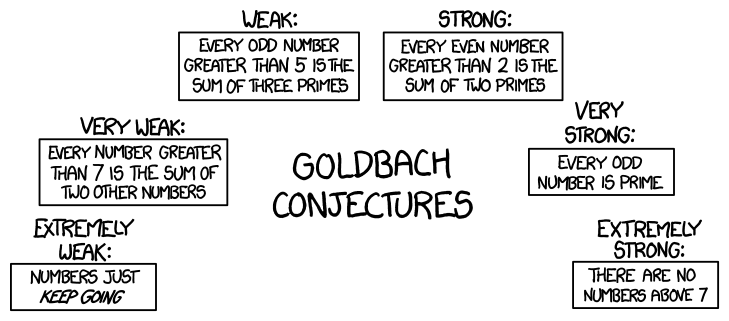
\includegraphics[width=0.5\textwidth]{background/pix/goldbach_conjectures.png}}
    \caption{Goldbach 的种种猜想。（致谢 \protect\href{https://xkcd.com/1310/}{\texttt{xkcd.com}}）}
    \label{fig:GoldbachsConjectures}
  \end{figure}
\end{answer}
\end{exercise}

\begin{exercise}
\definend{Brocard 问题}\index{Brocard's problem}
即是否存在除 $4$、$5$ 和~$7$ 以外的数，使得 $n!+1$ 是一个完全平方数
（计算机搜索最高已达
\citetext{一千万亿，即 $1\times 10^{15}$}{
  参见 \url{https://github.com/jhg023/brocard}.}，尚未发现其他解）。
证明：如果我们能够解决 \HP{}，那么我们原则上就能够判定这个问题。
\begin{answer}\verified
我们可以写一个程序，它接受输入，忽略输入，并执行一个循环来搜索大于~$7$ 的解，一旦找到就停机。
只要有了 \HP{} 的解法，我们就能检查该程序是否会停机，从而判定这个问题。
\end{answer}
\end{exercise}

% \begin{exercise}
% If we could solve the \HP{} then could we solve all problems?
% \begin{answer}
% No.
% \end{answer}
% \end{exercise}

\begin{exercise}
通过证明存在不可数无穷多个无法被任何 Turing 机计算的函数 $\map{f}{\N}{\N}$，而可计算的函数数量是可数的，来证明大多数问题都是不可解的。
\begin{answer}\verified
  所有函数 $\map{f}{\N}{\N}$ 的集合是两个子集的不交并：可计算的函数和不可计算的函数。
  我们知道可计算函数的集合是可数的。
  因为两个可数集的并集仍然是可数集，所以如果不可计算函数的集合也是可数的，那么总体上就只有可数多个函数，但事实并非如此。
  因此，不可计算函数的集合是不可数的。
\end{answer}
\end{exercise}

\begin{exercise}
给出一个全可计算函数（即对所有输入都收敛）的例子，使得其值域是不可计算的。
\begin{answer}
  固定一个元素 $k\in K$。
  以下函数 $\map{f}{\N^2}{\N}$ 的值域是~$K$。
  \begin{equation*}
    f(x,n)=
    \begin{cases}
    x  &\case{if $\TM_x$ with input~$x$ halts in $n$ steps}  \\
    k  &\case{otherwise}
    \end{cases}
  \end{equation*}
  显然该函数是可计算的，并且对所有输入对 $x,n\in\N^2$ 都收敛。
  对于 $K$ 的所有元素，都存在一个 $n$ 使得 $x$ 出现在值域中。
  同理，只有~$K$ 中的元素才会出现在值域中。
\end{answer}
\end{exercise}

\begin{exercise}
若一个比特串集合的特征函数是可计算的，则称其为
\definend{可判定语言}\index{decidable!language}\index{language!decidable}。
证明以下各条。
\begin{exparts*}
\item
两个可判定语言的并集是可判定语言。
\item
两个可判定语言的交集是可判定语言。
\item
一个可判定语言的补集是可判定语言。
\end{exparts*}
\begin{answer}\verified
  设有两个可判定语言~$\lang_0$ 和~$\lang_1$。
  因为它们是可判定的，所以存在 Turing 机 $\TM_{e_0}$ 和 $\TM_{e_1}$ 来判定其成员归属。
  \begin{equation*}
    \TMfcn_{e_0}(x)=
    \begin{cases}
      1  &\case{if $x\in\lang_0$}  \\
      0  &\case{if $x\notin\lang_0$}
    \end{cases}
    \qquad
    \TMfcn_{e_1}(x)=
    \begin{cases}
      1  &\case{if $x\in\lang_1$}  \\
      0  &\case{if $x\notin\lang_1$}
    \end{cases}
  \end{equation*}
  注意，这些机器在所有输入上都停机。
  \begin{figure}
    \centering
    \vcenteredhbox{\includegraphics{\asydir hp/hp1024.pdf}}
    \qquad
    \vcenteredhbox{\includegraphics{\asydir hp/hp1025.pdf}}
    \caption{判定可判定语言并集与交集的机器草图。}
    \label{fig:DecidableLangsUnionInt}
  \end{figure}
  \begin{exparts}
  \item
  判定 $\lang_0\cup\lang_1$ 成员资格的机器草图如 \figureref{fig:DecidableLangsUnionInt} 左侧所示。
  如果一个数是其中至少一个集合的成员，那么它就是并集的元素。
  因此，给定~$x$，这台机器首先在~$x$ 上运行 $\TM_{e_0}$。
  如果它返回~$1$，那么 $x$ 就是并集的成员，于是新机器输出~$1$。
  否则，新机器在~$x$ 上运行~$\TM_{e_1}$ 并返回其结果。
  \item
  判定 $\lang_0\cap\lang_1$ 成员资格的机器草图在同一图的右侧。
  如果一个数同时是这两个集合的成员，那么它就是交集的元素。
  因此，给定~$x$，这台机器首先在~$x$ 上运行 $\TM_{e_0}$。
  如果它返回~$0$，那么 $x$ 不是交集的成员，于是新机器输出~$0$。
  否则，新机器在~$x$ 上运行~$\TM_{e_1}$ 并返回其结果。
  \item
  补集的情况直截了当。
  对于~$\lang_0$ 的补集，新机器只需运行 $\TM_{e_0}$，并将其结果从~$1$ 中减去。
  \end{exparts}
\end{answer}
\end{exercise}


\end{exercises}
\index{Halting problem@\probname{Halting} problem|)}
\index{unsolvability|)}\index{unsolvable problem|)}

%================================================
\section{Rice 定理}\index{Rice's theorem|(}\label{sec:RicesThm}
我们在上一节最后指出，那里的结果和例子提供了一种直觉：我们无法
机械地分析 Turing 机的行为。
在本节中，我们将使这一直觉变得精确。

机械分析确实适用于 Turing 机的某些属性。
我们可以编写一个例程，给定~$e$，
判定 $\TM_e$ 是否有一条四元组指令，其第一项是状态~$q_5$。
在普通编程中，类似的情形是我们可以写一个程序来解析源代码，寻找名为 \str{x1} 的变量。
但这些并不是我们所说的“行为”。
相反，它们是实现层面的属性。

% A property is
% \definend{semantic}\index{semantic property}\index{property!semantic}
% if it has to do with the meaning of a thing; in our case,
% with what the machine does.\footnote{%
%   Often writers contrast these with properties that are
%   \definend{syntactic},\protect\index{syntactic property}\protect\index{property!syntactic}
%   which have to do with how a formal object is constructed.
%   We covered the syntax of Turing machines in the book's first section.}
% Briefly, a property is semantic if it is about $\TMfcn$ more than~$\TM\!$.
% For example,
% consider a Turing machine~$\TM$ that inputs a natural number and outputs~$1$
% if the number is prime and~$0$ otherwise.
% This machine's behavior is that it
% acts as the characteristic function of the set of primes.
% In contrast, suppose that it has a state~$q_5$ but no state~$q_6$.
% If we change all of the $q_5$'s in its transition table to some unused state
% such as $q_{1000}$'s
% then we get a different machine but the same behavior.

%<*def:SameBehavior>


\begin{definition}
两个可计算函数
\definend{具有相同行为，$\TMfcn_{e}\samebehavior\TMfcn_{\hat{e}}$}，\index{same behavior, functions with}\index{functions!same behavior}
如果它们在相同的输入~$x\in\N$ 上收敛，
且在收敛时具有相同的输出。\footnotemark[2]
\end{definition}

\footnotetext[2]{%
  严格来说，我们并不需要符号~$\samebehavior$。
  根据定义，函数是一个有序对的集合。
  如果
  $\TMfcn_e(0)\converges$ 而~$\TMfcn_e(1)\diverges$，那么集合 $\TMfcn_e$
  包含一个第一项为~$0$ 的有序对，但不包含任何第一项为~$1$ 的有序对。
  因此对于偏函数，如果它们在相同的输入上收敛，且在收敛时输出相同，那么我们可以直接说
  这两个函数相等，$\TMfcn=\hat{\TMfcn}$。
  但我们使用 $\samebehavior$ 来提醒自己这些函数可能是偏的。}
%</def:SameBehavior>

%<*def:IndexSet>


\begin{definition}
自然数集合 $\mathcal{I}$ 是一个
\definend{索引集}\footnotemark[1]\index{index set}\index{set!index}，
如果对所有~$e,\hat{e}\in\N$，
只要 $e\in\mathcal{I}$ 且 $\TMfcn_e\samebehavior\TMfcn_{\hat{e}}$，
则 $\hat{e}\in\mathcal{I}$ 也成立。
\end{definition}

\footnotetext[1]{%
  之所以称为索引集，是因为它是索引的集合。}
%</def:IndexSet>

\begin{example}
如果我们固定一种行为，并考虑所有具有该行为的 Turing 机
的索引，那么我们就得到了一个索引集。
因此，集合
$\mathcal{I}=\set{e\in\N\suchthat \text{$\phi_e(x)=2x$ for all $x$}}$
是一个索引集。
为了验证，假设 $e\in\mathcal{I}$ 且 $\hat{e}\in\N$ 满足
$\phi_e\samebehavior \phi_{\hat{e}}$。
那么 $\phi_{\hat{e}}$ 也将其输入翻倍：$\phi_{\hat{e}}(x)=2x$ 对所有~$x$ 成立。
因此 $\hat{e}\in\mathcal{I}$ 也成立。
\end{example}

\begin{example} \label{ex:IndexSetMultipleBehaviors}
我们也可以通过收集多种行为来得到一个索引集。
集合
$\mathcal{J}=\set{e\in\N\suchthat
      \text{$\phi_e(x)=3x$ for all $x$, or $\phi_e(x)=x^3$ for all~$x$}}
$
是一个索引集。
因为，假设 $e\in\mathcal{J}$ 且
$\phi_e\samebehavior \phi_{\hat{e}}$，其中 $\hat{e}\in\N$。
由于 $e\in\mathcal{J}\!$，要么
$\phi_e(x)=3x$ 对所有 $x$ 成立，要么 $\phi_e(x)=x^3$ 对所有~$x$ 成立。
从 $\phi_e\samebehavior \phi_{\hat{e}}$ 我们知道，
要么 $\phi_e(x)=3x$ 对所有 $x$ 成立，要么 $\phi_e(x)=x^3$ 对所有~$x$ 成立，从而
$\hat{e}\in\mathcal{J}\!$。
\end{example}

\begin{example} \label{ex:NotIndexSet}
集合 $\set{e\in\N\suchthat
      \text{$\TM_e$ contains an instruction starting with $q_{10}$}}$
不是一个索引集。
我们可以很容易地构造两台行为相同的 Turing 机，
其中一台包含这样一条指令，而另一台不包含。
\end{example}

%<*th:RicesTheorem>


\begin{theorem}[Rice 定理]\index{Rice's theorem}   \label{thm:RicesThm}
每个非平凡的索引集（即非空且不是全体自然数集~$\N$）都是不可计算的。
\end{theorem}


%</th:RicesTheorem>

\begin{proof}
%<*pf:RicesTheoremi>
设 $\mathcal{I}$ 是一个非平凡的索引集。
选取 $e\in\N$，使得 $\TMfcn_{e}(y)\diverges$ 对所有 $y$ 成立。
那么要么 $e\in\mathcal{I}$，要么 $e\notin\mathcal{I}$。
我们将证明在第二种情况下 $\mathcal{I}$ 是不可计算的。
第一种情况类似，留作练习~\zcref{exer:OtherHalfRicesThm}。

所以假设 $e\notin\mathcal{I}$。
由于 $\mathcal{I}$ 非空，它包含一个索引 $\hat{e}\in\mathcal{I}$。
因为 $\mathcal{I}$ 是一个索引集，$\TMfcn_{e}\not\simeq\TMfcn_{\hat{e}}$。
因此存在一个 $y$ 使得 $\TMfcn_{\hat{e}}(y)\converges$。

考虑下面的左流程图。
根据 Church 论题，存在一台具有该行为的 Turing 机。
记其为 $\TM_{e_0}$。
应用 \smn{} 定理将 $x$ 参数化，
得到一致可计算的函数族 $\TMfcn_{s(e_0,x)}$，其计算过程如右图所示。
%</pf:RicesTheoremi>
\begin{center}
  \vcenteredhbox{\includegraphics{\asydir hp/hp12.pdf}}
  \hspace{4em}
  \vcenteredhbox{\includegraphics{\asydir hp/hp13.pdf}}
\end{center}
%<*pf:RicesTheoremii>
我们构造了右边的机器，使得如果
$\TMfcn_x(x)\diverges$，那么 $\TMfcn_{s(e_0,x)}\samebehavior\TMfcn_{e}$，
从而 $s(e_0,x)\notin\mathcal{I}$。
同样，
如果 $\TMfcn_x(x)\converges$，那么 $\TMfcn_{s(e_0,x)}\samebehavior\TMfcn_{\hat{e}}$，
从而 $s(e_0,x)\in\mathcal{I}$。
由此可得，如果 $\mathcal{I}$ 是机械可计算的，从而我们能
有效检查是否 $s(e_0,x)\in\mathcal{I}$，
那么我们就能解决停机问题。
%</pf:RicesTheoremii>
\end{proof}

\begin{example}
我们将使用 Rice 定理证明此问题不可解：给定
$e$，判定 $\TMfcn_e(3)\converges$ 是否成立。
我们必须定义一个适当的集合~$\mathcal{I}$，然后验证它非空、
不等于全体自然数集，并且是一个索引集。

令
$
  \mathcal{I}=\set{e\in\N \suchthat \TMfcn_e(3)\converges}
$。
验证该集合非空的最简单方法是给出一个成员。
下面左侧的例程直觉上是可计算的，因此
根据 Church 论题，存在一台具有该行为的 Turing 机。
那台机器的索引是 $\mathcal{I}$ 的一个成员，
从而 $\mathcal{I}\neq\emptyset$。
\begin{center}
  \vcenteredhbox{\includegraphics{\asydir hp/hp1052.pdf}}
  \hspace{6em}
  \vcenteredhbox{\includegraphics{\asydir hp/hp1053.pdf}}
\end{center}
同样，为了验证 $\mathcal{I}$ 不包含每个数，
考虑右侧的例程。
Church 论题表明，存在一台具有该行为的 Turing 机。
那台机器的索引不是 $\mathcal{I}$ 的成员，
因此 $\mathcal{I}\neq\N$。

我们最后验证 $\mathcal{I}$ 是一个索引集。
假设 $e\in\mathcal{I}$，并令 $\hat{e}\in\N$ 满足 $\TMfcn_e\samebehavior\TMfcn_{\hat{e}}$。
由于 $e\in\mathcal{I}$，我们有 $\TMfcn_e(3)\converges$。
因为 $\TMfcn_e\samebehavior\TMfcn_{\hat{e}}$，我们也有
$\TMfcn_{\hat{e}}(3)\converges$，从而
$\hat{e}\in\mathcal{I}$。
因此 $\mathcal{I}$ 是一个索引集。
\end{example}

上面的例子与前一子节的第一个例子是同一个问题。
Rice 定理极大地简化了答案。
（当然，我们对这一定理的推导依赖于前节的工作。）

\begin{example}
我们可以用 Rice 定理来证明前一节的第二个问题不可解：给定 $e$，
判定是否存在某个 $x$ 使得 $\phi_e(x)=7$。
我们将构造一个适当的 $\mathcal{I}$
并验证它是一个非平凡的索引集。

令
$\mathcal{I}=\set{e\in\N \suchthat \text{$\TMfcn_e(x)=7$ for some $x$}}$。
这个集合非空，因为存在一台 Turing 机作为恒等函数，
即 $\TMfcn(x)=x$，
那台机器的索引是 $\mathcal{I}$ 的一个成员。
这个集合不等于全体自然数集，因为
存在一台永不停机的 Turing 机，对所有 $x$ 都有 $\TMfcn(x)\diverges$，
那台机器的索引不是 $\mathcal{I}$ 的成员。
因此 $\mathcal{I}$ 是非平凡的。

为了证明 $\mathcal{I}$ 是一个索引集，
假设 $e\in\mathcal{I}$，并令 $\hat{e}\in\N$ 满足
$\TMfcn_e\samebehavior\TMfcn_{\hat{e}}$。
由假设，存在某个输入 $x_0$ 使得 $\TMfcn_e(x_0)=7$。
由于两者具有相同行为，相同的输入会给出
$\TMfcn_{\hat{e}}(x_0)=7$。
因此，$\hat{e}\in\mathcal{I}$。
\end{example}

\begin{example}
这里是另一个不可解问题：给定~$e$，判定 $\TMfcn_e$ 是否等于 \begin{equation*}
  f(x)=
  \begin{cases}
    4  &\case{if $x$ is prime}  \\
    x+1 &\case{otherwise}
  \end{cases}
\end{equation*}。
令$\mathcal{I}=\set{j\in\N\suchthat \TMfcn_j=f}$。
集合~$\mathcal{I}$ 非空，因为我们可以写出具有这种行为的程序，因此根据 Church 论题，存在具有这种行为的 Turing 机，其索引就是~$\mathcal{I}$ 中的成员。
同时，$\mathcal{I}\neq\N$，因为存在一台在任何输入上都不停机的 Turing 机，它的索引不是~$\mathcal{I}$ 的成员。

为完成证明，我们论证~$\mathcal{I}$ 是一个索引集。
假设 $e\in\mathcal{I}$ 并且 $\hat{e}$ 满足 $\TMfcn_e\samebehavior\TMfcn_{\hat{e}}$。
因为 $e\in\mathcal{I}$，所以对所有输入~$x$ 均有 $\TMfcn_e(x)=f(x)$。
由于 $\TMfcn_e\samebehavior\TMfcn_{\hat{e}}$，我们对所有~$x$ 均有 $\TMfcn_{\hat{e}}(x)=\TMfcn_{e}(x)$，因此 $\hat{e}$ 也是~$\mathcal{I}$ 中的成员。
所以 $\mathcal{I}$ 是一个索引集。
\end{example}

最后，我们从一个稍高的层次重新审视这一定理。
本章首先展示了不可解问题是存在的。
然而，那个基于计数的证明并没有给出自然的例子。
在上一节中，我们得到了许多有趣且实用的不可解问题的例子，
这些例子让我们直观地认识到，我们无法机械地分析机器的行为。
本节我们形式化地定义了“行为”。
在此基础上，
Rice 定理指出，每一个有意义的行为集合，
即每一个非平凡索引集，都是不可解的。
因此，我们起初觉得不可解问题十分离奇，
接着认识到它们确实会出现，
直到现在，如果粗略地解读，甚至可能会让人觉得所有问题都是不可解的。

但这显然不对。
我们都编写过处理现实世界任务的程序，对于这些程序的行为，我们至少会非正式地认为它们是有趣的。
要化解这一矛盾，当然需要认识到 Rice 定理指出的只是：只有当问题属于特定类型时才是不可解的。
我们现在就来详述这种类型。

在下方的左图中，红点代表 Turing 机。
（当然机器的数量是无限的，但这只是一个示意图。）
有些成对的机器具有相同的输入/输出行为，也就是说它们
产生相同的可计算函数。\footnote{%
  实际上，第~\protect\pageref{lem:EveryCompFcnHasInfManyIndices}~页的 Padding 引理
  指出对于每个可计算函数都存在无穷多台机器。}
因此，存在多台机器其输入/输出行为是加倍函数 $f(x)=2x$，
多台机器在任何输入上都不停机，
等等。
图中的瓦片将具有相同行为、给出相同可计算函数的机器分在一组。


\begin{center}
  \includegraphics{\asydir indexsets/indexsets002.pdf}%
  \hspace*{4em}
  \includegraphics{\asydir indexsets/indexsets003.pdf}%
\end{center}

如果每当两台机器计算同一函数时——即每当它们出现在
同一块瓦片中时——它们要么都具有该性质，
要么都不具有，我们就说机器的这个性质是
\citetext{外延的}{%
  这个说法源自 A~Bauer，见 \url{https://cs.stackexchange.com/q/2811/67754}。\index{extensional property}
}。
Rice 定理断言，一个有效的（即可计算的）机器外延性质必须是平凡的，也就是说，它要么对所有机器都成立，要么对所有机器都不成立。

以下是机器的一些外延性质：


\begin{parenum}
\item 在输入~$3$ 上停机，
\item 存在一个输入使得输出为~$7$，
\item 存在一个输入使得机器不停机。
\end{parenum}


例如对于~(1)，由于它是一个
外延性质且非平凡，Rice 定理指出它不可能是
有效的，我们无法可计算地判定它。

以下是一些非外延性质，
Rice 定理对它们不适用：


\begin{parenum}
\item 在每个输入上都在 $100$ 步内停机，
\item 在输入~$0$ 上访问少于~$100$ 个带方格，以及
\item 包含状态~$q_{10}$。
\end{parenum}

那么，如果每个瓦片代表一种行为，什么是索引集呢？
正如我们之前所见，例如在 \zcref{ex:IndexSetMultipleBehaviors} 中，
一个索引集是多个瓦片的索引的并集；
右上方的图合并了其中的三个瓦片。
属于这个~$\mathcal{I}$ 这一性质是外延的，因为我们取的是
完整的瓦片。

总而言之，尽管 Rice 定理并不适用于所有问题，
但它对于理解仅凭机械分析能做什么具有特别重要的意义。
Rice 定理关注的是机器的这样一类性质，它们可以推广为机器所计算函数的性质。
例如，判定一个程序是否计算平方函数的问题是不可解的，
但判定其源代码是否包含字母 ‘\str{k}’ 的问题则不是。

% ...................................................
\begin{exercises}
% possible: https://cs.stackexchange.com/q/117066/50343

\begin{exercise}
你的朋友感到困惑，“根据 Rice 定理，所有事情都是不可能的。
计算机程序的每个性质都是不可计算的。
但我却一直在做这些本该不可能的事情！”
请帮他理清头绪。
\begin{credit}
  问题来自 StackExchange 用户 MathematicalOrchid，
  \url{https://cs.stackexchange.com/q/2811/67754},
  本节使用了 StackExchange 用户 Andrej Bauer 的答案。
  此处的答案并非来自 Andrej Bauer。
\end{credit}
\begin{answer}\verified
Rice 定理并没有说所有事情都是不可能的。
例如，它并没有说编写一个实现 $f(x)=x^2$ 的例程是不可能的。

它所断言不可能的事情是：编写一个例程，在给定源代码后，
能够正确判定这段源代码（无论写得多么巧妙，或故意混淆得多么晦涩）是否实现了~$f$。
（这种判定器之所以有意义，是因为我们可以把它应用到第一段提到的那个例程上，
从而确切地知道它在所有情况下都能正确工作。）
\end{answer}
\end{exercise}

\begin{exercise}
$\mathcal{I}=\set{e\suchthat \text{$\TM_e$ runs for at least $100$ steps on input~$5$}}$
是索引集吗？
\begin{answer}\verified
  不是，它不是索引集。
  我们可以写出两台行为相同的 Turing 机，例如，对任何输入~$x$，它们都输出~$x$。
  其中一台只需要很少几步就能做到这一点
  （平凡的 Turing 机~$\TM=\set{}$ 甚至只需零步），
  而另一台需要 $101$ 步。
  第二台机器的索引属于~$\mathcal{I}$，但第一台机器的索引不属于。
\end{answer}
\end{exercise}

\begin{exercise}
为什么 Rice 定理没有表明这个问题是不可解的：给定~$e$，判定是否
$\emptyset\subseteq\set{x\suchthat \TMfcn_e(x)\converges}$？
\begin{answer}\verified
使得
$\emptyset\subseteq\set{x\suchthat \TMfcn_e(x)\converges}$
成立的索引~$e\in\N$ 的集合是整个 $\N$。
这个问题是可解的，尽管其解是平凡的：对任何~$e$，答案都是“是”。
\end{answer}
\end{exercise}

\begin{exercise}
判断真假：以下关于机器的性质是外延的吗？简要说明理由。
\begin{exparts*}
\item 机器在输入~$5$ 上停机。
\item 它恰好有四条指令。
\item 它计算其输入的两倍。
\end{exparts*}
\begin{answer}\verified
\begin{exparts}
\item 真，这是关于机器的输入/输出行为的。
  如果两台机器具有相同的输入/输出行为，并且其中一台在输入~$5$ 上停机，
  那么另一台也必然如此。
\item 假，我们可以造出两台行为相同，但其中一台有四条指令而另一台没有四条指令的机器。
  例如，我们可以拿一台有四条指令的机器，然后通过添加不可达代码来造一台新机器，
  这些无实际作用的指令以原四条指令未曾引用过的状态为起始状态。
\item 真。
  如果两台机器计算相同的函数，并且第一台机器的函数是 $x\mapsto 2x$，
  那么第二台机器的函数也是如此。
\end{exparts}
\end{answer}
\end{exercise}

\begin{exercise}
简要说明为何本节列出的这些机器性质是非外延的。
\begin{exparts*}
\item 在任何输入上都能在 $100$ 步内停机的性质，
\item 在输入~$0$ 时访问少于~$100$ 个带方格的性质，以及
\item 包含状态~$q_{10}$ 的性质。
\end{exparts*}
\begin{answer}\verified
在每种情况下，我们都将论证：存在两台机器 $\TM$ 和~$\hat{\TM}$，
它们具有相同的输入/输出行为，$\TMfcn=\hat{\TMfcn}$，但其中一台机器具有该性质而另一台没有。
\begin{exparts}
\item 平凡的 Turing 机 $\TM=\set{}$ 在零步内停机，其行为是 $\TMfcn(x)=x$。
  我们可以轻易地造出另一台具有相同行为，但耗费超过一百步的机器。
\begin{equation*}
  \hat{\TM}=\set{
       \tminstruction{0}{B}{B}{1},
       \tminstruction{0}{1}{1}{1},
       \tminstruction{1}{B}{B}{2},
       \tminstruction{1}{1}{1}{2},
       \ldots\,
       \tminstruction{100}{B}{B}{101},
       \tminstruction{100}{1}{1}{101}
     }
\end{equation*}
\item 与上一条类似，平凡的机器在输入~$0$ 时使用零个带方格。
  下面这台机器在输入~$0$ 时访问一百零一个带方格。
\begin{equation*}
  \hat{\TM}=\set{
       \tminstruction{0}{B}{L}{1},
       \tminstruction{0}{1}{1}{102},
       \tminstruction{1}{B}{L}{2},
       \tminstruction{1}{1}{L}{2},
       \ldots\,
       \tminstruction{100}{B}{L}{101},
       \tminstruction{100}{1}{L}{101}
     }
\end{equation*}
  两台机器的行为相同，都是 $\TMfcn(x)=x$。
\item 平凡的机器不包含任何带有状态~$q_{10}$ 的指令。
  下面这台机器
\begin{equation*}
  \hat{\TM}=\set{\tminstruction{0}{B}{B}{1},
        \tminstruction{0}{1}{1}{1},
        \tminstruction{1}{B}{B}{2},
        \tminstruction{1}{1}{1}{2},
        \ldots\,
        \tminstruction{10}{B}{B}{11},
        \tminstruction{10}{1}{1}{11}
      }
\end{equation*}
  具有相同的行为，并且包含一条带有该状态的指令。
\end{exparts}
\end{answer}
\end{exercise}

\begin{exercise}
构造一个平凡的索引集：填空
$\mathcal{I}=\set{e\suchthat \text{\underline{\makebox[3em]{}}$\TM_e$\underline{\makebox[3em]{}}}}$
使得集合~$\mathcal{I}$ 是空集。
\begin{answer}\verified
  描述空集的方式有很多。
  一种是 $\set{e\suchthat \text{$\TM_e$ solves the \HP}}$。
\end{answer}
\end{exercise}

\begin{exercise}
构造一个平凡的索引集：填空
$\mathcal{I}=\set{e\suchthat \text{\underline{\makebox[3em]{}}$\TM_e$\underline{\makebox[3em]{}}}}$
使得集合~$\mathcal{I}$ 是整个 $\N$。
\begin{answer}\verified
  描述所有索引的集合~$\N$ 的一种方式是 $\set{e\suchthat \text{on input~$3$ machine $\TM_e$ either halts or does not}}$。
\end{answer}
\end{exercise}

\begin{exercise}
对于下列每个问题，构造一个适用于 Rice 定理的索引集。
你无需给出完整论证，只需给出这个集合即可。
\begin{exparts}
\item 给定 $e$，判断 $\TM_e$ 在输入 $7$ 上是否停机且输出 $7\!$。
\item 给定 $e$，判断 $\TM_e$ 在输入~$e$ 上是否停机且输出~$e$。
\item 给定 $e$，判断 $\TM_{2e}$ 是否对任意输入~$y$ 都输出 $7$。
\item 给定 $e$，判断 $\TM_e$ 在输入 $7$ 上是否停机并输出一个素数。
\end{exparts}
\begin{answer}\verified
记号 $\TMfcn_e(x)=y$ 表示 $\TMfcn_e(x)$ 收敛且输出值为~$y$。
\begin{exparts}
\item $\set{e\in\N\suchthat \text{$\TMfcn_e(7)=7$}}$
\item $\set{e\in\N\suchthat \text{$\TMfcn_e(e)=e$}}$
\item $\set{e\in\N\suchthat \text{there is a $y$ where $\TMfcn_{2e}(y)=7$}}$
\item $\set{e\in\N\suchthat \text{$\TMfcn_e(7)\converges$ and is prime}}$
\end{exparts}
\end{answer}
\end{exercise}

\exerciseinstructions{对于 \zcref{exer:FirstRiceExercise} 到 \zcref{exer:FinalRiceExercise} 中的每个问题，通过应用 Rice 定理来证明它是不可解的。（这些问题重复了 \zcref{exer:FirstReduceExercise} 到 \zcref{exer:FinalReduceExercise} 的问题。）}

\recommended


\begin{exercise}\label{exer:FirstRiceExercise}
\refexerciseinstructions{}
给定
索引~$e$，
判断 $\TMfcn_e$ 是否为全函数，即它是否在每个输入上都收敛。
\begin{answer}\verified
令 $\mathcal{I}=\set{e\in\N\suchthat\text{$\TMfcn_e$ is total}}$。
我们将证明它是一个非平凡的索引集。

首先证明~$\mathcal{I}$ 不是空集。
考虑 \figureref{fig:INotTrivialTotalFcnsNotComputable} 左侧草图所示的程序。
  \begin{figure}
    \centering
    \vcenteredhbox{\includegraphics{\asydir hp/hp1028.pdf}}
    \hspace*{4em}
    \vcenteredhbox{\includegraphics{\asydir hp/hp1029.pdf}}
    \caption{用于证明集合~$\mathcal{I}$ 非平凡的机器。}
    \label{fig:INotTrivialTotalFcnsNotComputable}
  \end{figure}
根据 Church 论题，存在一台符合此草图的 Turing 机。
它有一个索引，且该索引是~$\mathcal{I}$ 的元素。
所以 $\mathcal{I}$ 非空。

接下来证明~$\mathcal{I}$ 不是整个~$\N$。
考虑同一图右侧草图所示的程序。
根据 Church 论题，存在一台符合此草图的 Turing 机。
它的索引不是~$\mathcal{I}$ 的元素，因此
$\mathcal{I}$ 不是整个~$\N$。

最后，我们证明 $\mathcal{I}$ 是一个索引集。
假设 $e\in\mathcal{I}$ 且 $\hat{e}$ 满足 $\TMfcn_e\samebehavior\TMfcn_{\hat{e}}$。
因为 $e\in\mathcal{I}$，
我们知道对所有的 $a\in\N$ 有 $\TMfcn_e(a)\converges$。
由于 $\TMfcn_x\samebehavior\TMfcn_{\hat{e}}$，我们因此知道
对所有的 $a\in\N$ 有 $\TMfcn_{\hat{e}}(a)\converges$。
于是，$\hat{e}\in\mathcal{I}$，从而
$\mathcal{I}$ 是一个索引集。

因此，Rice 定理表明，
判定“全函数性”的问题，即给定~$e$ 时判定
Turing 机~$\TM_e$ 是否在所有输入上停机的问题，
是不可解的。
\end{answer}
\end{exercise}

\recommended


\begin{exercise}
\refexerciseinstructions[exer:FirstRiceExercise]
给定索引~$e$，判定 Turing 机~$\TM_e$ 是否计算其输入的平方。
也就是说，判定 $\TMfcn_e$ 是否实现映射 $y\mapsto y^2$。
\begin{answer}\verified
令 $\mathcal{I}=\set{e\in\N\suchthat\text{$\TMfcn_e(y)=y^2$ for all $y$}}$。
我们将证明它是一个非平凡的索引集。

首先证明~$\mathcal{I}$ 不是空集。
考虑 \figureref{fig:INotTrivialSquarerFcnsNotComputable} 左侧草图所示的程序。
  \begin{figure}
    \centering
    \vcenteredhbox{\includegraphics{\asydir hp/hp1030.pdf}}
    \hspace*{4em}
    \vcenteredhbox{\includegraphics{\asydir hp/hp1031.pdf}}
    \caption{用于证明平方函数的索引集 $\mathcal{I}$ 非平凡的机器。}
    \label{fig:INotTrivialSquarerFcnsNotComputable}
  \end{figure}
根据 Church 论题，存在一台符合此草图的 Turing 机。
它有一个索引，且该索引是~$\mathcal{I}$ 的元素。
所以 $\mathcal{I}$ 非空。

接下来证明~$\mathcal{I}$ 不是整个~$\N$。
考虑同一图右侧草图所示的程序。
根据 Church 论题，存在一台符合此草图的 Turing 机。
它的索引不是~$\mathcal{I}$ 的元素，因此
$\mathcal{I}$ 不是整个~$\N$。

最后我们证明 $\mathcal{I}$ 是一个索引集。
假设 $e\in\mathcal{I}$ 且 $\hat{e}$ 满足 $\TMfcn_e\samebehavior\TMfcn_{\hat{e}}$。
因为 $e\in\mathcal{I}$，
我们知道对所有 $y\in\N$ 有 $\TMfcn_e(y)=y^2$。
由于 $\TMfcn_e\samebehavior\TMfcn_{\hat{e}}$，我们因此知道
对所有 $y\in\N$ 有 $\TMfcn_{\hat{e}}(y)=y^2$。
于是，$\hat{e}\in\mathcal{I}$，从而
$\mathcal{I}$ 是一个索引集。

由此，Rice 定理表明，
给定~$e$，判定 Turing 机~$\TM_e$ 是否计算其输入的平方的问题，
是不可解的。
\end{answer}
\end{exercise}

\begin{exercise}
\refexerciseinstructions[exer:FirstRiceExercise]
给定~$e$，确定函数~$\TMfcn_e$ 是否在两个相邻输入上返回相同的值，
即存在某个~$y\in\N$ 使得 $\TMfcn_e(y)=\TMfcn_e(y+1)$。
\begin{answer}\verified
我们将证明
$\mathcal{I}=\set{e\in\N\suchthat\text{$\TMfcn_e(y)=\TMfcn_e(y+1)$ for some $y\in\N$}}$
是一个非平凡的索引集。

首先证明~$\mathcal{I}$ 非空。
考虑 \figureref{fig:IRepeatedValueFcnNotTrivial} 左侧草图所示的程序。
  \begin{figure}
    \centering
    \vcenteredhbox{\includegraphics{\asydir hp/hp1028.pdf}}
    \hspace*{4em}
    \vcenteredhbox{\includegraphics{\asydir hp/hp1029.pdf}}
    \caption{用于证明集合~$\mathcal{I}$ 非平凡的机器。}
    \label{fig:IRepeatedValueFcnNotTrivial}
  \end{figure}
它在直观上是可计算的，因此根据 Church 论题，存在一台符合此草图的 Turing 机。
该 Turing 机的索引是~$\mathcal{I}$ 的一个元素。
所以 $\mathcal{I}$ 非空。

接下来论证~$\mathcal{I}\neq\N$。
考虑同一图右侧草图所示的程序。
根据 Church 论题，存在一台符合此草图的 Turing 机。
它的索引不是~$\mathcal{I}$ 的元素，因此 $\mathcal{I}$ 不是整个~$\N$。

最后，证明 $\mathcal{I}$ 是一个索引集。
假设 $e\in\mathcal{I}$，并且 $\hat{e}$ 满足 $\TMfcn_e\samebehavior\TMfcn_{\hat{e}}$。
因为 $e\in\mathcal{I}$，存在 $y\in\N$ 使得 $\TMfcn_e(y)=\TMfcn_e(y+1)$。
由于 $\TMfcn_e\samebehavior\TMfcn_{\hat{e}}$，我们知道对于同一个~$y$，有 $\TMfcn_{\hat{e}}(y)=\TMfcn_{\hat{e}}(y+1)$。
因此，$\hat{e}\in\mathcal{I}$。
所以 $\mathcal{I}$ 是一个索引集。

于是，根据 Rice 定理，
判定是否属于 $\mathcal{I}$ 的问题是不可解的。
\end{answer}
\end{exercise}

\begin{exercise}
\refexerciseinstructions[exer:FirstRiceExercise]
给定索引~$e$，确定 $\TMfcn_e$ 在输入~$5$ 上是否发散。
\begin{answer}\verified
我们将证明
$\mathcal{I}=\set{e\in\N\suchthat\TMfcn_e(5)\diverges}$
是一个非平凡的索引集。

首先证明~$\mathcal{I}\neq\emptyset$。
考虑 \figureref{fig:IDivergesOnFiveNotTrivial} 左侧草图所示的程序。
  \begin{figure}
    \centering
    \vcenteredhbox{\includegraphics{\asydir hp/hp1029.pdf}}
    \hspace*{4em}
    \vcenteredhbox{\includegraphics{\asydir hp/hp1028.pdf}}
    \caption{用于证明~$\mathcal{I}$ 非平凡的 Turing 机草图。}
    \label{fig:IDivergesOnFiveNotTrivial}
  \end{figure}
它在直观上是可计算的，因此根据 Church 论题，存在一台符合此草图的 Turing 机。
该机器的索引是~$\mathcal{I}$ 的一个元素。

接下来论证~$\mathcal{I}\neq\N$。
考虑同一图右侧草图所示的程序。
根据 Church 论题，存在一台符合此草图的 Turing 机。
它的索引不是~$\mathcal{I}$ 的元素。

最后，证明 $\mathcal{I}$ 是一个索引集。
假设 $e\in\mathcal{I}$，并且 $\hat{e}$ 满足 $\TMfcn_e\samebehavior\TMfcn_{\hat{e}}$。
因为 $e\in\mathcal{I}$，我们知道 $\TMfcn_e(5)\diverges$。
但 $\TMfcn_e\samebehavior\TMfcn_{\hat{e}}$，所以我们也有 $\TMfcn_{\hat{e}}(5)\diverges$。
因此，$\hat{e}\in\mathcal{I}$。
所以 $\mathcal{I}$ 是一个索引集。

由此，Rice 定理表明判定是否属于 $\mathcal{I}$ 的问题是不可解的。
\end{answer}
\end{exercise}

\begin{exercise}
\refexerciseinstructions[exer:FirstRiceExercise]
给定一个索引，确定 Turing 机 $\TM_e$ 是否在所有奇数上均不停机。
\begin{answer}\verified
我们将证明
$\mathcal{I}=\set{e\in\N\suchthat\text{$\TMfcn_e(y)\diverges$ for all odd~$y$}}$
是一个非平凡的索引集。

首先证明~$\mathcal{I}\neq\emptyset$。
考虑 \figureref{fig:IDivergesOnOddNotTrivial} 左侧草图所示的程序。
  \begin{figure}
    \centering
    \vcenteredhbox{\includegraphics{\asydir hp/hp1029.pdf}}
    \hspace*{4em}
    \vcenteredhbox{\includegraphics{\asydir hp/hp1028.pdf}}
    \caption{用于证明~$\mathcal{I}$ 非平凡的机器。}
    \label{fig:IDivergesOnOddNotTrivial}
  \end{figure}
它在直观上是可计算的，因此根据 Church 论题，存在一台符合此草图的 Turing 机。
该机器的索引是~$\mathcal{I}$ 的一个元素。

接下来验证~$\mathcal{I}\neq\N$。
考虑同一图右侧草图所示的程序。
根据 Church 论题，存在一台符合此草图的 Turing 机。
它的索引不是~$\mathcal{I}$ 的元素。

最后，证明 $\mathcal{I}$ 是一个索引集。
假设 $e\in\mathcal{I}$，并且 $\hat{e}$ 满足 $\TMfcn_e\samebehavior\TMfcn_{\hat{e}}$。
因为 $e\in\mathcal{I}$，我们知道对于所有奇数输入~$y$，$\TMfcn_e(y)\diverges$。
由于 $\TMfcn_e\samebehavior\TMfcn_{\hat{e}}$，我们也知道对于所有奇数~$y$，$\TMfcn_{\hat{e}}(y)\diverges$。
因此，$\hat{e}\in\mathcal{I}$，
所以 $\mathcal{I}$ 是一个索引集。

由此，Rice 定理表明判定是否属于 $\mathcal{I}$ 的问题是不可解的。
\end{answer}
\end{exercise}

\begin{exercise}
\refexerciseinstructions[exer:FirstRiceExercise]
给定索引~$e$，判断由机器~$\TM_e$ 计算的函数~$\phi_e$ 是否实现映射 $x\mapsto x+1$。
\begin{answer}\verified
我们将证明
$\mathcal{I}=\set{e\in\N\suchthat\TMfcn_e(x)=x+1}$
是一个非平凡的索引集。

首先证明~$\mathcal{I}\neq\emptyset$。
考虑 \figureref{fig:ISuccessorNotTrivial} 左侧的程序草图。
  \begin{figure}
    \centering
    \vcenteredhbox{\includegraphics{\asydir hp/hp1032.pdf}}
    \hspace*{4em}
    \vcenteredhbox{\includegraphics{\asydir hp/hp1033.pdf}}
    \caption{用于证明~$\mathcal{I}$ 非平凡的机器。}
    \label{fig:ISuccessorNotTrivial}
  \end{figure}
它直观上是可计算的，因此由 Church 论题，存在一台 Turing 机符合此草图。
该机器的索引是~$\mathcal{I}$ 的一个元素。

接着证明~$\mathcal{I}\neq\N$。
考虑该图右侧的程序草图。
由 Church 论题，存在一台 Turing 机符合此草图。
它的索引不是~$\mathcal{I}$ 的元素。

最后证明 $\mathcal{I}$ 是一个索引集。
假设 $e\in\mathcal{I}$ 并且 $\hat{e}$ 满足
$\TMfcn_e\samebehavior\TMfcn_{\hat{e}}$。
因为 $e\in\mathcal{I}$，我们知道对所有输入~$x$ 都有 $\TMfcn_e(x)=x+1$。
由于 $\TMfcn_e\samebehavior\TMfcn_{\hat{e}}$，我们也知道
$\TMfcn_{\hat{e}}(x)=x+1$ 对所有~$x$ 成立。
因此，$\hat{e}\in\mathcal{I}$。
所以 $\mathcal{I}$ 是一个索引集。

于是，由 Rice 定理，
判定~$\mathcal{I}$ 的成员资格问题是不可解的。
\end{answer}
\end{exercise}

\begin{exercise} \label{exer:FinalRiceExercise}
\refexerciseinstructions[exer:FirstRiceExercise]
给定索引~$e$，判断函数~$\phi_e$ 是否对某个~$x$，在输入 $x$ 和~$2x$ 上均发散。
\begin{answer}\verified
我们将证明
$\mathcal{I}=\set{e\in\N\suchthat\text{both $\TMfcn_e(x)\diverges$ and $\TMfcn_e(2x)\diverges$ for some~$x$}}$
是一个非平凡的索引集。

首先证明~$\mathcal{I}\neq\emptyset$。
考虑 \figureref{fig:IDivergesOnXAndTwoXNotTrivial} 左侧的程序草图。
  \begin{figure}
    \centering
    \vcenteredhbox{\includegraphics{\asydir hp/hp1034.pdf}}
    \qquad
    \vcenteredhbox{\includegraphics{\asydir hp/hp1035.pdf}}
    \caption{用于证明~$\mathcal{I}$ 非平凡的机器。}
    \label{fig:IDivergesOnXAndTwoXNotTrivial}
  \end{figure}
它直观上是可计算的，因此由 Church 论题，存在一台 Turing 机符合此草图。
该机器的索引是~$\mathcal{I}$ 的一个元素。

接着证明~$\mathcal{I}\neq\N$。
考虑 \figureref{fig:IDivergesOnXAndTwoXNotTrivial} 右侧的程序草图。
由 Church 论题，存在一台 Turing 机符合此草图。
它的索引不是~$\mathcal{I}$ 的元素。

最后证明 $\mathcal{I}$ 是一个索引集。
假设 $e\in\mathcal{I}$ 并且 $\hat{e}$ 满足
$\TMfcn_e\samebehavior\TMfcn_{\hat{e}}$。
因为 $e\in\mathcal{I}$，我们知道存在某个输入~$x$，使得 $\TMfcn_e(x)\diverges$ 且 $\TMfcn_e(2x)\diverges$。
由于 $\TMfcn_e\samebehavior\TMfcn_{\hat{e}}$，我们知道对同一个~$x$，
$\TMfcn_{\hat{e}}(x)\diverges$ 且 $\TMfcn_{\hat{e}}(2x)\diverges$。
因此，$\hat{e}\in\mathcal{I}$。
所以 $\mathcal{I}$ 是一个索引集。

于是，由 Rice 定理，
判定~$\mathcal{I}$ 的成员资格问题是不可解的。
\end{answer}
\end{exercise}

\recommended


\begin{exercise}
应用 Rice 定理，证明下列每个问题都是不可解的。
\begin{exparts}
\item 判定一个函数是否为偏函数，即该函数是否在某个输入上发散。
\item 判定一个函数是否至少在某个输入上收敛。
\end{exparts}
\begin{answer}\verified
第一小题中的索引集，是 \ref{exer:FirstRiceExercise} 中那个索引集的补集。
  后续练习 \ref{exer:IndexSetsClosedSetOps} 会证明，索引集的补集也是索引集。
  但下面我们将不依赖这些练习，
  直接验证所给问题是不可解的。
\begin{exparts}
\item  问题是：给定索引~$e$，
  判定是否存在 $y\in\N$ 使得~$\TMfcn_e(y)\diverges$。
  为了证明它是不可解的，我们要验证 $\mathcal{I}=\set{e\in\N\suchthat
                     \text{$\TMfcn_e(y)\diverges$ for some $y\in\N$}}$
  是一个非平凡索引集。

  集合~$\mathcal{I}$ 非空，因为我们可以写一个在所有输入上都不停机的程序，
  然后由 Church 论题知，存在具有该行为的 Turing 机。
  该机器的索引属于~$\mathcal{I}$。

  该集合不等于全体自然数~$\N$，
  因为我们可以写一个程序，它直接返回其输入值，
  并由 Church 论题知，存在具有该行为的 Turing 机。
  该机器的索引不是~$\mathcal{I}$ 的成员。

  最后我们来验证~$\mathcal{I}$ 是一个索引集。
  假设 $e\in\mathcal{I}$，并且 $\hat{e}$ 满足 $\TMfcn_{e}\samebehavior\TMfcn_{\hat{e}}$。
  因为 $e\in\mathcal{I}$，我们知道存在至少一个
  $y\in\N$ 使得 $\TMfcn_e(y)\diverges$。
  由于两者行为相同，
  $\TMfcn_{\hat{e}}(y)\diverges$ 对至少一个~$y$ 也成立。
  因此 $\hat{e}\in\mathcal{I}$，于是 $\mathcal{I}$ 是索引集。
\item
  令 $\mathcal{I}=\set{e\in\N\suchthat
                     \text{$\TMfcn_e(y)\converges$ for some $y\in\N$}}$。
  我们将验证它是一个非平凡索引集。

  集合~$\mathcal{I}$ 非空，因为我们可以写一个在所有输入上都输出~$0$ 的程序。
  由 Church 论题可知，存在具有该行为的 Turing 机。
  该机器的索引属于~$\mathcal{I}$。

  集合~$\mathcal{I}$ 不等于全体自然数~$\N$，因为我们可以写一个在任何输入上都不停机的程序，
  再由 Church 论题，存在具有该行为的 Turing 机，并且该机器的索引不属于~$\mathcal{I}$。

  在确认了 $\mathcal{I}$ 是非平凡的之后，我们来完成最后一步，验证它是索引集。
  假设 $e\in\mathcal{I}$，并且 $\hat{e}$ 满足 $\TMfcn_{e}\samebehavior\TMfcn_{\hat{e}}$。
  因为 $e\in\mathcal{I}$，我们知道存在至少一个
  $y\in\N$ 使得 $\TMfcn_e(y)\converges$。
  由于两者行为相同，因此 $\TMfcn_{\hat{e}}(y)\converges$ 对至少一个~$y$ 也成立。
  因此 $\mathcal{I}$ 是一个索引集。
\end{exparts}
\end{answer}
\end{exercise}

\recommended


\begin{exercise}
对于每个问题，请填空以证明其不可解性。
\begin{quotation}\it
\quad 我们将证明
$\mathcal{I}=\set{e\in\N\suchthat\text{\fillinblankLabelled{(1)}}}$
是一个非平凡索引集。
然后，根据 Rice 定理，判定~$\mathcal{I}$ 的成员资格问题是算法不可解的。

\quad 首先我们论证 $\mathcal{I}\neq\emptyset$。
这里给出的程序草图：\fillinblankLabelled{(2)}
在直观上是可计算的，因此依据 Church 论题，存在这样的 Turing 机。
那台机器的索引就是 $\mathcal{I}$ 的一个元素。

\quad 接下来论证 $\mathcal{I}\neq\N$。
另一个程序草图：\fillinblankLabelled{(3)}
同样是直观可计算的，因此依据 Church 论题，存在这样的 Turing 机。
这台机器的索引不是 $\mathcal{I}$ 的元素。

\quad 最后，我们证明 $\mathcal{I}$ 是一个索引集。
假设 $e\in\mathcal{I}$，并且 $\hat{e}$ 满足
$\TMfcn_e\samebehavior\TMfcn_{\hat{e}}$。
由于 $e\in\mathcal{I}$，可知 \fillinblankLabelled{(4)}。
因为 $\TMfcn_e\samebehavior\TMfcn_{\hat{e}}$，可得
\fillinblankLabelled{(5)}。
因此，$\hat{e}\in\mathcal{I}$。
所以 $\mathcal{I}$ 是一个索引集。
\end{quotation}
\begin{exparts}
\item 给定索引~$e$，判定 Turing 机~$e$ 是否对所有是 5 的倍数的输入~$x$ 都停机。
\item 给定索引~$e$，判定 Turing 机~$e$ 是否曾输出 7。
\end{exparts}
\begin{answer}\verified
每个答案仅给出对应编号的填空。
\begin{exparts}
\item
(1)~$\TMfcn_e(x)\converges$ 对所有是 5 的倍数的输入~$x$ 皆成立。
(2)~及~(3) 见 \figureref{fig:FillInBlankIMultsOfFive}。
  \begin{figure}
    \centering
    \vcenteredhbox{\includegraphics{\asydir hp/hp1036.pdf}}
    \hspace*{4em}
    \vcenteredhbox{\includegraphics{\asydir hp/hp1037.pdf}}
    \caption{用于论证 $\mathcal{I}$ 非平凡性的机器。}
    \label{fig:FillInBlankIMultsOfFive}
  \end{figure}
(4)~$\TMfcn_e(5k)\converges$ 对所有~$k\in\N$ 成立。
(5)~$\TMfcn_{\hat{e}}(5k)\converges$ 对所有~$k\in\N$ 也成立。
\item
(1)~存在某个输入~$x$ 使得 $\TMfcn_e(x)=7$。
(2)~及~(3) 见 \figureref{fig:FillInBlankIEverOutputSeven}。
  \begin{figure}
    \centering
    \vcenteredhbox{\includegraphics{\asydir hp/hp1038.pdf}}
    \hspace*{4em}
    \vcenteredhbox{\includegraphics{\asydir hp/hp1039.pdf}}
    \caption{用于论证 $\mathcal{I}$ 非平凡性的机器。}
    \label{fig:FillInBlankIEverOutputSeven}
  \end{figure}
(4)~存在某个~$x\in\N$ 使得 $\TMfcn_e(x)=7$。
(5)~$\TMfcn_{\hat{e}}(x)=7$ 对同一个~$x$ 成立。
\end{exparts}
\end{answer}
\end{exercise}

\begin{exercise}
证明任何不可计算集都是无限集。
\begin{answer}\verified
所有有限集都是可计算的。
对于有限集，我们可以很容易地写出一个程序来充当其特征函数；只需考虑有限多种情况。
（依据 Church 论题，若存在这样的程序，就存在这样的 Turing 机。）
\end{answer}
\end{exercise}

\begin{exercise}
定义：若一台 Turing 机输入比特串，在所有输入上都停机，且当且仅当输入是~$\lang$ 的成员时输出~$1$，则称该机
\definend{判定}\index{Turing machine!decide a language}\index{language!decided by a Turing machine}
一个比特串集合 $\lang\subseteq\kleenestar{\B}$。
用 Rice 定理证明下列问题不可解。
\begin{exparts*}
\item
给定 $e\in\N$，判定 $\TM_e$ 是否判定一个无限语言。
\item
给定 $e\in\N$，判定 $\TM_e$ 是否接受串 \str{101}。
\end{exparts*}
\begin{answer}\verified
  \begin{exparts}
  \item
  我们将证明这是一个非平凡索引集：
  $\mathcal{I}=\set{e\in\N\suchthat \text{$\TM_e$ decides an infinite language}}$。

  首先验证 $\mathcal{I}$ 非空。
  我们可以构造一台对所有输入都输出~$1$ 的 Turing 机，该机接受 $\lang=\B$ 中的每一个串，而该集合是无限集。
  因此该 Turing 机的索引属于~$\mathcal{I}$。

  其次验证 $\mathcal{I}$ 不等于~$\N$。
  我们可以构造一台对所有输入都输出~$0$ 的 Turing 机。
  该机接受空集，而空集不是无限集。
  因此该 Turing 机的索引不是~$\mathcal{I}$ 的元素。

  最后，为验证 $\mathcal{I}$ 是索引集，假设
  $e\in\mathcal{I}$ 且 $\hat{e}\in\N$ 满足
  $\TMfcn_e\samebehavior\TMfcn_{\hat{e}}$。
  由于 $e\in\mathcal{I}$，$\TM_e$ 判定一个无限语言。
  因为 $\TMfcn_e\samebehavior\TMfcn_{\hat{e}}$，$\TM_{\hat{e}}$ 输出~$1$ 的比特串集合等于
  $\TM_e$ 输出~$1$ 的集合，所以 $\TM_{\hat{e}}$ 也判定一个无限语言。
  因此 $\hat{e}\in\mathcal{I}$，且 $\mathcal{I}$ 是索引集。
  \item
  我们将证明
  $\mathcal{I}=\set{e\in\N\suchthat \text{$\TM_e$ 接受 \str{101}}}$
  是一个非平凡索引集。
  首先，$\mathcal{I}$ 非空，因为我们可以构造一台对所有输入都输出~$1$ 的 Turing 机，该机接受串~\str{101}。
  该机的索引是~$\mathcal{I}$ 的一个元素。

  其次，$\mathcal{I}$ 不等于~$\N$，因为我们可以构造一台对所有输入都输出~$0$ 的 Turing 机，该机不接受串~\str{101}。
  该机的索引不是~$\mathcal{I}$ 的元素。

  最后，验证 $\mathcal{I}$ 是索引集。
  假设 $e\in\mathcal{I}$ 且 $\hat{e}\in\N$ 满足
  $\TMfcn_e\samebehavior\TMfcn_{\hat{e}}$。
  因为 $e\in\mathcal{I}$，机器 $\TM_e$ 接受~\str{101}。
  因为 $\TMfcn_e\samebehavior\TMfcn_{\hat{e}}$，
  机器 $\TM_{\hat{e}}$ 也接受~\str{101}。
  因此 $\hat{e}\in\mathcal{I}$，且 $\mathcal{I}$ 是索引集。
  \end{exparts}
\end{answer}
\end{exercise}

\begin{exercise}
如同前一练习，若一台 Turing 机输入比特串，在所有输入上都停机，且当输入是~$\lang$ 的成员时输出~$1$，否则输出~$0$，则称它
\definend{接受}
一个比特串集合 $\lang\subseteq\kleenestar{\B}$。
证明下列问题不可解：给定~$e$，
判定 $\TM_e$ 是否接受 $\kleenestar{\B}$ 本身。
证明下列问题是机械不可解的：给定~$e$，判定是否存在输入~$x$ 使得~$\TMfcn_e(x)\converges$。
\begin{answer}\verified
  我们用 Rice 定理，考虑
  $\mathcal{I}=\set{e\suchthat  \text{$\TM_e$ accepts every $\sigma\in\kleenestar{\B}$}}$。

  首先，我们可以构造一台在所有输入上都停机并输出~$1$ 的 Turing 机，该机的索引是~$\mathcal{I}$ 的成员，所以 $\mathcal{I}$ 不是空集。

  其次，我们可以构造一台在所有输入上都停机并输出~$0$ 的 Turing 机，该机的索引不是~$\mathcal{I}$ 的成员，所以 $\mathcal{I}\neq\N$。

  为证明 $\mathcal{I}$ 是索引集，
  假设 $e\in\mathcal{I}$ 且自然数~$\hat{e}$ 满足 $\TMfcn_e\samebehavior\TMfcn_{\hat{e}}$。
  因为 $e\in\mathcal{I}$，机器 $\TM_e$ 接受所有比特串。
  因为 $\TMfcn_e\samebehavior\TMfcn_{\hat{e}}$，机器 $\TM_{\hat{e}}$ 也
  接受所有比特串。
  因此 $\hat{e}\in\mathcal{I}$，且 $\mathcal{I}$ 是非平凡索引集。
\end{answer}
\end{exercise}

\begin{exercise}
若对于所有输入，机器在计算过程中都从未进入该状态，则称该 Turing 机有一个
\definend{不可达状态}\index{unreachable state}\index{state!unreachable}。
证明
$\mathcal{I}=\set{e\suchthat \text{$\TM_e$ has an unreachable state}}$
不是索引集。
\begin{answer}\verified
我们可以构造两台 Turing 机 $\TM_e$ 和~$\TM_{\hat{e}}$，
它们具有相同行为，$\TMfcn_e\samebehavior\TMfcn_{\hat{e}}$，
但 $e\in\mathcal{I}$ 而 $\hat{e}\notin\mathcal{I}$。
下面是两台这样的机器。
\begin{equation*}
  \TM_e =
  \set{\tminstruction{0}{B}{B}{0},
       \tminstruction{0}{1}{1}{0},
       \tminstruction{1}{B}{B}{1},
       \tminstruction{1}{1}{1}{1}
      }
  \qquad
  \TM_{\hat{e}} =
  \set{\tminstruction{0}{B}{B}{0},\tminstruction{0}{1}{1}{0}}
\end{equation*}
第一台具有不可达状态 $q_1$。
\end{answer}
\end{exercise}

\begin{exercise}
\begin{credit}
  \href{https://cs.stackexchange.com/q/86660}{SE 用户 Rajesh R}
  % https://cs.stackexchange.com/users/78255/rajesh-r), Whether TM accepts epsilon?, URL (version: 2018-01-13):
\end{credit}
你的同学说：“这一节最后说 Rice 定理是关于那些延伸为机器所计算的函数性质的机器性质。
但这里有一个问题，它也是关于机器性质的，并且是可解的：给定~$e$，判断 $\TM_e$ 是否仅在空输入带上停机。
要解决这个问题，给机器~$\TM_e$ 提供空输入，看它是停机还是继续运行。”
他们错在哪里？
\begin{answer}\verified
  这个问题是不可解的。
  我们不能通过机器是否“继续运行”（即没有立即停止）来判断任何事情。
  它可能继续做相当复杂的事情然后最终停止，或者做复杂的事情并且永远不停止。

  进一步地，我们可以将 \HP{} 归约到这个问题。
  考虑这个 $\map{\psi}{\N^2}{\N}$。
  \begin{equation*}
    \psi(x,y)=
    \begin{cases}
      42  &\case{if machine $\TM_x$ halts on~$x$ and $y=\emptystring$}  \\
      \uparrow &\case{otherwise}
    \end{cases}
  \end{equation*}
  （我们设这台机器的纸带字母表为
  $\Sigma=\set{\str{B},\str{1}}$。）
  这直观上是可计算的，所以由 Church 论题，存在一台具有该行为的 Turing 机，
  并且我们可以假设它的索引是~$e_0$。

  应用 \smn{} 定理对~$x$ 进行参数化，
  给出一族机器和相关的可计算函数，如下所示。
  \begin{equation*}
     \TMfcn_{s(e_0,x)}(y)=
     \begin{cases}
       42 &\case{if machine $\TM_x$ halts on~$x$ and $y=\emptystring$}  \\
      \uparrow &\case{otherwise}
     \end{cases}
  \end{equation*}
  那么 $\TMfcn_x(x)\converges$ 当且仅当函数
  $\TMfcn_{s(e_0,x)}$ 只在 $y=\emptystring$ 上停机。
  所以如果我们能机械地检查后者，那么我们就能机械地解决 \HP，
  这当然是不可能的。
\end{answer}
\end{exercise}

\begin{exercise}
证明任何非空有限集都不是索引集。
\begin{answer}\verified
填充引理（I.\ref{lem:EveryCompFcnHasInfManyIndices}）说每个可计算函数都有无限多个索引。
所以如果集合包含一个 $e\in\N$，那么它必须包含无限多个
索引~$\hat{e}$，使得 $\TMfcn_e\samebehavior\TMfcn_{\hat{e}}$。
\end{answer}
\end{exercise}

\begin{exercise}
证明以下每个集合都是索引集。
\begin{exparts}
\item
$\set{e\in\N\suchthat \text{machine $\TM_e$ halts on at least five inputs}}$
\item
$\set{e\in\N\suchthat \text{the function $\TMfcn_e$ is one-to-one}}$
\item
$\set{e\in\N\suchthat \text{the function $\TMfcn_e$ is either total or else $\TMfcn_e(3)\diverges$}}$
\end{exparts}
\begin{answer}\verified
  我们称每个集合为~$\mathcal{I}$。
  \begin{exparts}
  \item 假设 $e\in\mathcal{I}$ 且 $\hat{e}$ 满足
  $\TMfcn_{e}\samebehavior\TMfcn_{\hat{e}}$。
  因为 $e\in\mathcal{I}$，机器 $\TM_e$ 至少在五个输入上停机，
  即函数 $\TMfcn_e$ 至少在五个输入上收敛。
  因为 $\TMfcn_{e}\samebehavior\TMfcn_{\hat{e}}$，函数
  $\TMfcn_{\hat{e}}$ 也至少在五个输入上停机，即相同的这五个输入。
  因此 $\hat{e}\in\mathcal{I}$。
  \item 假设 $e\in\mathcal{I}$ 且 $\hat{e}\in\N$ 满足
  $\TMfcn_{e}\samebehavior\TMfcn_{\hat{e}}$。
  因为 $e\in\mathcal{I}$，函数 $\TMfcn_e$ 是一一的。
  因为 $\TMfcn_{e}\samebehavior\TMfcn_{\hat{e}}$，函数
  $\TMfcn_{\hat{e}}$ 也是一一的。
  因此 $\hat{e}\in\mathcal{I}$。
  \item 假设 $e\in\mathcal{I}$ 且 $\hat{e}\in\N$ 满足
  $\TMfcn_{e}\samebehavior\TMfcn_{\hat{e}}$。
  因为 $e\in\mathcal{I}$，函数 $\TMfcn_e$
  要么是全函数，要么 $\TMfcn_e(3)\diverges$。
  若 $\TMfcn_e$ 是全函数，
  因为 $\TMfcn_{e}\samebehavior\TMfcn_{\hat{e}}$，函数
  $\TMfcn_{\hat{e}}$ 也是全函数。
  若 $\TMfcn_e(3)\diverges$，
  因为它们行为相同，$\TMfcn_{\hat{e}}(3)\diverges$ 也发散。
  无论哪种情况，$\hat{e}\in\mathcal{I}$。
  \end{exparts}
\end{answer}
\end{exercise}

\begin{exercise}
在本节中，我们用下图刻画了索引集。
我们从全体整数的集合（即矩形框）开始，
当某些整数是相同可计算函数的索引时，就将它们分在一组。
然后，为了得到一个索引集，
选取其中的几个部分（如图中所示的三个），
并取它们的并集。
\begin{center}
  \vcenteredhbox{\includegraphics{\asydir indexsets/indexsets003.pdf}}
\end{center}
这里我们来验证这一图示的合理性。
\begin{exparts*}
\item
考虑自然数之间的如下关系 $\simeq$：
如果 $\phi_e\samebehavior\phi_{\hat{e}}$，则 $e\mathbin{\simeq}\hat{e}$。
证明这是一个等价关系。
\item
描述这些部分，即等价类。
\item
证明每个索引集都是一些等价类的并集。
\hint~证明如果一个索引集包含某个等价类的一个元素，
那么它包含该类的所有元素。
\end{exparts*}
\begin{answer}\verified
  \begin{exparts}
  \item
  关系~$\simeq$ 是自反的，
  因为 Turing 机 $\TM_e$ 与自身具有相同行为：$\phi_e\samebehavior\phi_e$。
  它是对称的，
  因为如果 $\TM_e$ 与 $\TM_{\hat{e}}$ 行为相同，
  那么反之也成立。
  传递性同样显然。
  \item
  每个等价类都是由自然数 $e\in\N$ 组成的集合。
  如果对应的 Turing 机 $\TM_e$ 和 $\TM_{\hat{e}}$
  的输入-输出行为相同，即~$\phi_e\samebehavior\phi_{\hat{e}}$，
  那么$e,\hat{e}\in\mathcal{C}$这两个整数就同属一个等价类。
  （例如，一个等价类包含所有将输入加倍的 Turing 机的索引，
  即$\mathcal{C}=\set{e\in\N\suchthat \text{$\phi_e(x)=2x$ for all $x$}}$。）
  \item
  我们按照提示来证明。
  假设~$\mathcal{I}$ 是一个索引集，
  $e$ 是~$\mathcal{I}$ 的一个元素，
  并且它属于关系~$\samebehavior$ 的等价类~$\mathcal{C}$。
  令 $\hat{e}$ 是类~$\mathcal{C}$ 的另一个元素，
  因此 $\TMfcn_{\hat{e}}\samebehavior\TMfcn_e$。
  因为 $\mathcal{I}$ 是一个索引集，所以 $\hat{e}\in\mathcal{I}$ 也成立。
  因此，如果 $\mathcal{I}$ 包含 $\mathcal{C}$ 的一个元素，
  那么它包含~$\mathcal{C}$ 的每一个元素。
  \end{exparts}
\end{answer}
\end{exercise}

\begin{exercise} \label{exer:IndexSetsClosedSetOps}
由于“是索引集”是集合的一种性质，
我们自然会考虑它与集合运算之间的相互作用。
\begin{exparts*}
\item
证明一个索引集的补集也是一个索引集。
\item
证明索引集族在并运算下封闭。
\item
它在交运算下封闭吗？
若是，请证明；若否，请给出反例。
\end{exparts*}
\begin{answer}\verified
  \begin{exparts}
  \item 设 $\mathcal{I}$ 是一个索引集，并考虑其补集~$\setcomp{\mathcal{I}}\!$。
  假设 $e\in\setcomp{\mathcal{I}}$，
  并且假设 $\hat{e}\in\N$ 满足 $\TMfcn_e\samebehavior\TMfcn_{\hat{e}}$。
  我们将证明 $\hat{e}\in\setcomp{\mathcal{I}}\!$。

  要么 $\hat{e}\in\mathcal{I}$，
  要么 $\hat{e}\in\setcomp{\mathcal{I}}\!$。
  若 $\hat{e}\in\mathcal{I}$，
  则由 $\TMfcn_e\samebehavior\TMfcn_{\hat{e}}$
  及 $\mathcal{I}$ 是一个索引集，
  可得 $e\in\mathcal{I}$ 也成立。
  这与假设 $e\in\setcomp{\mathcal{I}}\!$ 矛盾。
  因此 $\hat{e}\in\setcomp{\mathcal{I}}\!$。
  \item
  取一族索引集 $\mathcal{I}_j$，
  考虑并集 $\mathcal{I}=\cup_j\mathcal{I}_j$。
  假设 $e\in\mathcal{I}$，
  并且假设 $\hat{e}\in\N$ 满足 $\TMfcn_e\samebehavior\TMfcn_{\hat{e}}$。
  我们将证明 $\hat{e}\in\mathcal{I}$。

  数~$e$ 是并集 $\cup_j\mathcal{I}_j=\mathcal{I}$ 的一个元素，
  因此它是某个 $\mathcal{I}_{j_0}$ 的元素。
  因为 $\TMfcn_e\samebehavior\TMfcn_{\hat{e}}$ 且 $\mathcal{I}_{j_0}$ 是一个索引集，
  数~$\hat{e}$ 是 $\mathcal{I}_{j_0}$ 的一个元素，
  因此也是并集~$\mathcal{I}$ 的一个元素。
  所以 $\mathcal{I}$ 是一个索引集。
  \item
  它在交运算下封闭。
  设 $\mathcal{I}_j$ 是一族索引集，并令
  $\mathcal{I}=\cap_j\mathcal{I}_j$。
  假设 $e\in\mathcal{I}$，
  并且假设 $\hat{e}\in\N$ 满足 $\TMfcn_e\samebehavior\TMfcn_{\hat{e}}$。
  我们将证明 $\hat{e}\in\mathcal{I}$。

  由于~$e$ 是交集的一个元素，
  即 $\cap_j\mathcal{I}_j=\mathcal{I}$，所以它是每个集合 $\mathcal{I}_{j}$ 的元素。
  因为 $\TMfcn_e\samebehavior\TMfcn_{\hat{e}}$ 且每个 $\mathcal{I}_{j}$ 是一个索引集，
  数~$\hat{e}$ 也是每个 $\mathcal{I}_{j}$ 的元素。
  既然 $\hat{e}$ 是每个 $\mathcal{I}_{j}$ 的元素，
  它也是交集~$\mathcal{I}$ 的元素。
  因此 $\mathcal{I}$ 是一个索引集。
  \end{exparts}
\end{answer}
\end{exercise}

\begin{exercise}  \label{exer:OtherHalfRicesThm}
完成 Rice 定理（\zcref{thm:RicesThm}）证明中 $e_0\in\mathcal{I}$ 情况的证明。
\begin{answer}\verified
  本节中已完成的那一半证明先固定了一个索引 $e_0\in\N$，使得对所有的输入 $y\in\N$，$\TMfcn_{e_0}(y)\diverges$。
  然后处理了 $e_0\notin\mathcal{I}$ 的情况，因此这里剩下的工作是处理 $e_0\in\mathcal{I}$ 的情况。

  因为 $\mathcal{I}$ 是非平凡的，它不等于 $\N$。
  所以存在某个 $\hat{e}\notin\mathcal{I}$。
  由于 $\mathcal{I}$ 是一个索引集，$\TMfcn_{e_0}\not\simeq\TMfcn_{\hat{e}}$。
  因此存在某个 $y$ 使得 $\TMfcn_{\hat{e}}(y)\converges$。

  考虑 \figureref{fig:HalfRicesTheorem} 左侧的流程图。
  根据 Church 论题，存在一台具有该行为的 Turing 机；将其记为 $\TM_{e}$。
  应用 \smn 定理将 $x$ 参数化，得到了一致可计算的函数族 $\TMfcn_{s(e,x)}$，其计算过程由 \figureref{fig:HalfRicesTheorem} 右侧概述。
  \begin{figure}
    \centering
    \vcenteredhbox{\includegraphics{\asydir hp/hp12.pdf}}
    \hspace{4em}
    \vcenteredhbox{\includegraphics{\asydir hp/hp13.pdf}}
    \caption{证明一半 Rice 定理所用的机器示意图。}
    \label{fig:HalfRicesTheorem}
  \end{figure}
  我们构造这些机器时，使得如果 $\TMfcn_x(x)\diverges$，那么 $\TMfcn_{s(e,x)}\samebehavior\TMfcn_{e_0}$，从而 $s(e,x)\in\mathcal{I}$。
  进一步，如果 $\TMfcn_x(x)\converges$，那么 $\TMfcn_{s(e,x)}\samebehavior\TMfcn_{\hat{e}}$，从而 $s(e,x)\notin\mathcal{I}$。
  因此，如果 $\mathcal{I}$ 是机械可计算的，从而我们能够有效地检验是否 $s(e,x)\in\mathcal{I}$，那么我们就能机械地解决停机问题。
  当然，这是不可能的。
\end{answer}
\end{exercise}


\end{exercises}
\index{Rice's theorem|)}

% ========================================
\section{可计算枚举集合}\index{computably enumerable|(}\index{set!computably enumerable|(}\label{sec:ComputablyEnumerableSets}
% Required for the section on oracles.

处理停机问题的自然方法是，先模拟 $\TM_0$ 在输入 $0$ 上运行一步。
接着，模拟 $\TM_0$ 在输入 $0$ 上运行第二步，同时也模拟 $\TM_1$ 在输入 $1$ 上运行第一步。
然后，运行 $\TM_0$ 在输入 $0$ 上的第三步，$\TM_1$ 在输入 $1$ 上的第二步，接着运行 $\TM_2$ 在输入 $2$ 上的第一步。
以此类推，在 $\TM_e$ 关于输入 $e$ 的所有模拟中交替循环，每次让每个模拟各运行一步。\footnote{%
    也就是说，运行一个循环，在第 $i$ 次迭代时，运行模拟 $\TM_e$ 在输入 $e$ 上的第 $s$ 步，
    其中 $i=e+s$。
  }
最终其中一些会停机，$K$ 的元素便开始逐渐显现。
在计算机系统中，这种交错称为时间片轮转，但在理论讨论中称为
\citetext{\definend{交错并行（dovetailing）}}{% https://commons.wikimedia.org/wiki/File:Joinery-throughdovetail.svg
  木匠或木工使用燕尾榫来制作牢固的木制抽屉。
  它以一种交错互锁的方式编织两边，如下图所示。
  \protect

\begin{center}
  \protect\small
  \protect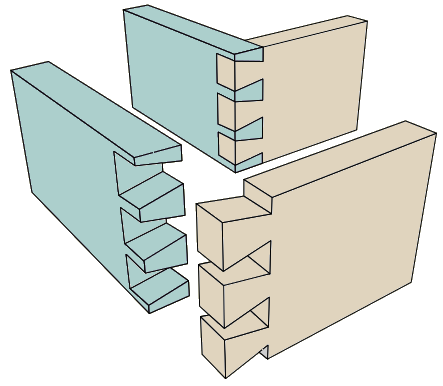
\includegraphics[width=0.15\textwidth]{background/pix/dovetail.png}
  \protect\end{center}

}。\index{dovetailing}

我们设想存在一个可计算函数 $f$，使得 $f(0)=e$，其中 $\TM_e$ 在输入 $e$ 上恰好是这些交错并行模拟中最先停机的那个，等等。
% And, $f(1)=\hat{e}$, where
% $\TM_{\hat{e}}$ on input~$\hat{e}$ is the second to halt in the dovetailing, etc.
数字流 $f(0)$、$f(1)$、\ldots{} 给出了 $K$ 的元素。

为什么这个过程解决不了停机问题呢？
如果 $e\in K$，那么交错并行最终会发现这一点。
但如果 $e\notin K$，那么它永远也无法揭示其非成员身份。

%<*def:ComputableSet>
回想一下，一个数集是可计算的\index{computable!set}\index{set!computable}% or decidable,\index{decidable!set}\index{set!decidable}，
如果其特征函数是可计算的。
%</def:ComputableSet>
我们看到了描述集合的另一种方式，% other than giving a criteria for membership,
即列出其成员。
\zcref{def:Countable} 给出了相应的术语：定义域为 $\N$ 的函数 $f$ 可“枚举”其值域。

%<*def:ComputablyEnumerable>


\begin{definition}  \label{def:ComputablyEnumerable}
一个自然数集合是
\definend{可计算枚举的}\index{computably enumerable set}\index{set!computably enumerable}\index{set!c.e.}\index{computably enumerable sets CE@computably enumerable sets \compclass{CE}}
（或 \definend{c.e.}）\@\index{c.e. set|see{computably enumerable}}，
如果它是可有效列出的，也就是说，如果它是一个可计算函数的值域。
（该函数可以是部分的。）
同义词有：
\definend{递归可枚举的}\index{recursively enumerable set|see{computably enumerable set}}\index{set!recursively enumerable|see{computably enumerable set}}\index{set!r.e.|see{computably enumerable set}}
（或 \definend{r.e.}），\@\index{r.e. set|see{computably enumerable set}}
或 \definend{半可计算的}\index{semicomputable set}\index{set!semicomputable}，
或 \definend{半可判定的}\index{semidecidable set}\index{set!semidecidable}。
由所有可计算枚举集合构成的集合记为
\citetext{$\compclass{RE}$}{%
  使用这个缩写而不是 “$\compclass{CE}$” 是因为，
  历史上“递归可枚举”曾是标准术语。}。
\end{definition}


%</def:ComputablyEnumerable>

想象由 $\TMfcn(0)$, $\TMfcn(1)$, $\TMfcn(2)$,~\ldots{} 构成的“流”逐渐填满这个集合。
（流中可能包含重复的数字，出现的顺序可能杂乱无章而不一定递增，也可能从某个点起所有的 $\TMfcn(i)$ 都发散。）

\begin{remark}
这里有一个特别有趣的“流”。
固定一个数学主题，比如初等数论。
该主题中的命题是符号串，我们可以给每个命题赋予一个编号
（例如，将该命题用 Unicode 表示，其编号即为二进制编码，并在二进制数前添加一个~\str{1}，以避免前导~\str{0} 带来的歧义）。
建立一个过程，以该主题的公理为起点，
对从这些公理出发的所有逻辑推导进行广度优先遍历。
它可能首先将公理~0 与公理~1 组合，然后将公理~0 与公理~2 组合，依此类推。
这样，它就生成了该理论所有可能证明的列表。
每当完成一个证明，该过程就输出推导中最终命题（即被证明的命题）的编号。

假设我们对这个主题中的某个命题感兴趣，
例如 \definend{Goldbach 猜想}\index{Goldbach's conjecture}（每个偶数都是至多两个素数之和）。
我们可以观察这个过程如何枚举定理。
如果该命题是可证明的，那么它的编号最终会出现。
\end{remark}

%<*lem:CEIffDomainOfComputableFcn>


\begin{lemma} \label{lem:CEIffDomainOfComputableFcn}
对于一个自然数集，下列条件等价。
\begin{thmparts}
\item 它是可计算枚举的，即它是某个可计算函数的值域。\label{itemA:lem:CEIffDomainOfComputableFcn}
\item 它是某个全可计算函数的值域，或者它是空集。\label{itemB:lem:CEIffDomainOfComputableFcn}
\item 它是某个可计算函数的定义域。
\end{thmparts}
\end{lemma}


%</lem:CEIffDomainOfComputableFcn>

\begin{proof}
我们来证明第一项和第二项等价。
第二项和第三项等价则是 \zcref{exer:CEIffDomainOfComputableFcn} 的内容。

（\ref{itemB:lem:CEIffDomainOfComputableFcn}）推（\ref{itemA:lem:CEIffDomainOfComputableFcn}）的方向是容易的。
若集合~$S$ 是某个全可计算函数的值域，那么它自然是某个可计算函数的值域。
如果 $S$ 是空集，那么它是某个永不收敛的可计算函数的值域。

现在证明（\ref{itemA:lem:CEIffDomainOfComputableFcn}）推（\ref{itemB:lem:CEIffDomainOfComputableFcn}）。
假设 $S$ 是可计算枚举的，
因此它是某个可计算函数~$\TMfcn_e$（可能不是全函数）的值域。
如果 $\TMfcn_e$ 对所有输入都发散，那么 $S=\emptyset$，这符合（\ref{itemB:lem:CEIffDomainOfComputableFcn}）中的一种情况。

另一种情况是 $\TMfcn_e$ 并非对所有输入都发散，此时我们将构造一个全可计算函数~$f$，使其值域为~$S$。
这种情况下，存在一个输入~$y$ 使得 $\TMfcn_e(y)\converges$。
令 $f(0)=\TMfcn_e(y)$。
至于函数的其他值：给定 $n\in\N$，在输入~$0$, $1$, \ldots, $n$ 上分别运行 $\TM_e$ 的计算，各运行 $n$ 步。
其中一些计算可能会停机。
设 $f(n)$ 为满足以下条件的最小 $k$：$\TM_e$ 在某个输入~$i\leq n$ 上于 $n$ 步内停机并输出~$k$，并且满足 $k\notin\set{f(0),f(1),\ldots\, f(n-1)}$。
如果不存在这样的~$k$，则令 $f(n)=s_0$。

由上一段最后一句话可知，$f$ 是全函数。
我们必须验证 $f$ 的值域就是~$S$。
对于 $t\in\N$，如果 $t\notin S$，那么 $\TM_e$ 永远不会输出它，因此 $t$ 永远不会等于某个~$f(n)$。
如果 $t\in S$，那么必然存在一个足够大的~$n$，使得 $\TM_e$ 在某个输入~$i\leq n$ 上于 $n$ 步内停机并输出~$t$。
此时，数~$t$ 就被 $f$ “排队等待输出”，这意味着它至多作为 $f(n+t)$ 被枚举出来。
\end{proof}

因此，可以有效列举的集合类，与可计算函数的定义域构成的类是相同的。
对于后者有一个标准记号。

%<*def:WSubE>


\begin{definition}
\definend{$W_e=\set{x\suchthat \TMfcn_e(x)\converges}$}
\end{definition}


%</def:WSubE>

%<*description:DecidableAndSemidecidable>
可计算集合与可计算枚举集合的区别在于：
集合~$S$ 是可计算的，如果存在一台 Turing 机能够判定其成员资格，
即输入一个数~$x$，并判定 $x\in S$ 是“是”还是“否”。
但对于可计算枚举集合，给定某个~$x$，我们可以建立一台机器来监视那个数字流，
如果 $x$ 出现，那么这台机器就判定为“是”。
然而，它可能永远也无法发现“否”。
% (Although there may well be another process that gets no's,
% as the next result notes.)
换一种说法，
一个集合是可计算的，如果存在一台 Turing 机能够同时识别成员与非成员；
而
一个集合是可计算枚举的，如果存在一台 Turing 机能够识别成员。
%</description:DecidableAndSemidecidable>

\begin{lemma}  \label{lem:ComputableAndCE}
\begin{thmparts}
\item \label{lem:SetComputableThenSetCE}
%<*lem:ComputableAndCEi>
  如果一个集合是可计算的，那么它是可计算枚举的。
%</lem:ComputableAndCEi>
\item \label{lem:SetComputableIffSetAndCompCE}
%<*lem:ComputableAndCEii>
  一个集合是可计算的，当且仅当它和它的补集都是可计算枚举的。
%</lem:ComputableAndCEii>
\end{thmparts}
\end{lemma}

\begin{proof}
对于~(\ref{lem:SetComputableThenSetCE})，令 $S\subseteq\N$ 是可计算的，因此其特征函数是一个可计算函数~$\TMfcn$。
我们将枚举~$S$ 的元素。
首先使用 $\TMfcn$ 来检验 $0\in S$ 是否成立，即 $\TMfcn(0)=1$ 是否成立。
然后检验 $1\in S$ 是否成立，以此类推。
如果这一系列检验最终找到某个 $k_0$ 使得 $\TMfcn(k_0)=1$，
则令 $f(0)=k_0$。
之后，迭代进行：通过检验 $k_0+1\in S$、 $k_0+2\in S$、\ldots{} 来寻找 $S$ 的下一个元素，
如果这一系列检验最终找到某个 $k_1$，则令 $f(1)=k_1$。
显然~$f$ 是一个值域为~$S$ 的可计算函数。

至于 (\ref{lem:SetComputableIffSetAndCompCE})，
首先假设 $S$ 是可计算的。
其补集 $\setcomp{S}$ 也是可计算的，因为
$\charfcn{\setcomp{S}}(x)=1-\charfcn{S}(x)$ 对所有~$x$ 成立。
由此，根据第~(\ref{lem:SetComputableThenSetCE}) 项，$S$ 和 $\setcomp{S}$ 都是可计算枚举的。

反之，
假设 $S$ 和 $\setcomp{S}$ 都是可计算枚举的。
设 $S$ 由函数~$g$ 枚举，$\setcomp{S}$ 由 $\hat{g}$ 枚举。
为证明 $S$ 是可计算的，我们将给出一个有效过程，它充当 $S$ 的特征过程，也就是说，给定~$x\in\N$，该过程能判定~$x\in S$ 是否成立。
思路是交错并行这两个枚举：首先让 $g(0)$ 的计算运行一步，同时让 $\hat{g}(0)$ 的计算也运行一步。
接下来，让 $g(0)$ 和 $\hat{g}(0)$ 的计算各进行第二步，同时让 $g(1)$ 和 $\hat{g}(1)$ 的计算各进行一步。
以这种方式继续下去，
最终我们将发现 $x$ 被枚举进入了 $S$ 或~$\setcomp{S}\!$ 中的一个。
\end{proof}

%<*lem:HPIsCE>


\begin{corollary} \label{cor:KCompNotCE}
\HP{} 集 $K$ 是可计算枚举的。\index{K, the Halting problem set@$K$, the Halting problem set}
其补集 $\setcomp{K}$ 则不是。
\end{corollary}


%</lem:HPIsCE>

\begin{proof}
集合~$K$ 是
$f(x)=\TMfcn_x(x)$
的定义域，
根据 Church 论题，这是一个偏可计算函数。
所以 $K$ 是可计算枚举的。
如果补集~$\setcomp{K}$ 也是可计算枚举的，那么
\zcref{lem:ComputableAndCE} 将推出 $K$ 是可计算的，
但事实并非如此。
\end{proof}

这个结果给出了关注可计算枚举集的一个理由，即
\HP{} 集~$K$ 属于这类集合，
像集合
$\set{e\suchthat \TMfcn_e(3)\converges}$
和 $\set{e\suchthat \text{there is an $x$ so that $\TMfcn_e(x)=7$}}$ 也是如此。
所以，可计算枚举集构成的类包含了许多有趣的成员。

这些集合令人感兴趣的另一个原因是哲学上的：考虑到 Church 论题，我们可以意识到，在某种意义上，可计算集是我们能够完全了解的唯一一类集合。
与这种认识相一致，可计算枚举集正是我们至少拥有部分信息的集合：我们能判定哪些元素在其中，但未必能判定哪些元素不在其中。

% .......................................
\begin{exercises}
\recommended


\begin{exercise}
一次小测上有一道题要求你定义“可计算枚举”。
一位朋友说他回答的是：
“一个可以由 Turing 机枚举，但不是可计算的集合。”
这回答正确吗？
\begin{answer}\verified
 只对了一半。
 若一个集合能被 Turing 机枚举就是可计算枚举的，这是对的。
 但“不是可计算的”是错的。
 例如，偶数集是可计算枚举的，因为它显然可以有效列举，同时它也是可计算的，因为其特征函数是可计算的。
\end{answer}
\end{exercise}

\begin{exercise}
你的学伴问大家：“空集是一个可计算枚举集。
但空集不是有效列举的，因为你没法列举‘没有东西’。”
他/她的思路哪里出了岔子？
\begin{answer}\verified
“有效列举”的意思是，某个机器过程将其作为输出集合给出。
有些 Turing 机无论输入什么都不会停机，
这些机器所枚举的就是空集。
\end{answer}
\end{exercise}

\recommended


\begin{exercise}
对于每一小问，构造一个能枚举它的函数。
\begin{exparts*}
\item $\N$
\item 偶数集
\item 完全平方数集
\item 集合 $\set{5,7,11}$。
\end{exparts*}
\begin{answer}\verified
对于每一小问，我们将给出一个可计算的全函数 $\map{f}{\N}{\N}$，使其值域为给定集合。
\begin{exparts}
  \item 恒等函数 $f(x)=x$ 即可。
  \item 函数 $f(x)=2x$ 即可。
  \item $f(x)=x^2$
  \item 这个函数可行。
  \begin{equation*}
     f(x)=
     \begin{cases}
       5  &\case{if $x=0$}  \\
       7  &\case{if $x=1$}  \\
      11  &\case{otherwise}
     \end{cases}
  \end{equation*}
  \end{exparts}
\end{answer}
\end{exercise}

\begin{exercise}
对以下各项，分别构造一个枚举它们的函数
\begin{exparts*}
\item 素数
\item 各位数字非递增的自然数
  （例如 $531$ 或 $5331$，但 $513$ 不符合）。
\end{exparts*}
\begin{answer}\verified
  对每一项，我们构造一个有效函数 $\map{f}{\N}{\N}$。
  \begin{exparts}
  \item 对应关系 $n\mapsto\text{$n$-th prime}$ 是一个函数。
    显然我们可以编写一个程序来计算它，因此由 Church 论题可知它是有效的。
  \item 为了计算这个函数，我们可以采用暴力搜索：给定~$n$，
    遍历自然数 $0$, $1$, \ldots{}\,，检查每个数的各位数字是否按非递增顺序出现，
    输出第 $n$ 个这样的数。
  \end{exparts}
\end{answer}
\end{exercise}

\begin{exercise}
是否存在无限的可计算枚举集？
有限的呢？
空集呢？
所有自然数的集合呢？
\begin{answer}\verified
以上四种情况都存在。
对于第一种和第四种情况，
我们可以编写一台 Turing 机，其输入/输出行为即为恒等函数 $x\mapsto x$，
这台机器枚举了所有的自然数。
因此，所有自然数的集合是可计算枚举的。

对于第二种和第三种情况，存在在任何输入上都不停机的 Turing 机，
所以空集是可计算枚举的。
\end{answer}
\end{exercise}

\begin{exercise}
以下两个集合中，一个是可计算的，另一个是可计算枚举但不可计算的。
哪个是哪个？
\begin{exparts}
\item $\set{e\suchthat \text{$\TM_e$ halts on input~$4$ in less than twenty steps}}$
\item $\set{e\suchthat \text{$\TM_e$ halts on input~$4$ in more than twenty steps}}$
\end{exparts}
\begin{answer}\verified
  第一个是可计算的，因为要判定一个数~$e$ 是否属于这个集合，我们只需要模拟二十步。
  第二个是可计算枚举但不可计算的。
  它是可计算枚举的，因为我们可以对索引 $e\in\N$ 进行交错并行计算。
  它是不可计算的，因为显然如果我们能解决它，我们就能解决判定 $\set{e\suchthat \TMfcn_e(4)\converges}$ 的成员归属问题，但由 Rice 定理可知我们无法解决那个问题。
\end{answer}
\end{exercise}

\begin{exercise}
下列集合哪些是可判定的，哪些是半可判定但不可判定的，哪些两者都不是？
用一句话论证。
\begin{exparts*}
\item
索引~$e$ 的集合，其中 $\TM_e$ 在输入~$7$ 上的运行步骤超过 $100$。
\item
索引~$e$ 的集合，其中 $\TM_e$ 在输入~$7$ 上的运行步骤少于 $100$。
\end{exparts*}
\begin{answer}\verified
对于集合来说，“可判定的”与“可计算的”含义相同，即其特征函数是全可计算函数。
同时，“半可判定的”与“可计算枚举的”含义相同。
\begin{exparts}
\item
这个集合是可计算的，因为我们只需要运行机器一百步。
由于它是可计算的，所以它也是可计算枚举的。
\item
这个集合也是可计算的，同样因为我们只需要运行机器一百步。
由于它是可计算的，所以它也是可计算枚举的。
\end{exparts}
\end{answer}
\end{exercise}

\begin{exercise} \autocite{GATE22}
以下两个陈述中，有一个是真的。
是哪一个？
\begin{exparts*}
\item 任何可计算枚举集的真子集都是可计算的。
\item 如果一个集合及其补集都是可计算枚举的，那么两者都是可计算的。
\end{exparts*}
\begin{answer}\verified
第二个陈述为真，由引理 \zcref{lem:ComputableAndCE} 即得。
第一个陈述为假；例如，集合~$\N$ 是可计算枚举的，
但其真子集 $K$ 不是可计算的。
\end{answer}
\end{exercise}

\recommended


\begin{exercise}
网上有人说，
“每个可数集~$S$ 都是可计算枚举的，因为如果 $\map{f}{\N}{\N}$ 的值域是~$S$，那么你就有了 $S$ 的枚举，即 $f(0)$, $f(1)$, \ldots”\sentencespace
解释为什么这是错的。
\begin{answer}\verified
  这个函数确实是一个枚举，但除非它是可计算的，否则这就不是可计算枚举。
  一个可数但不可计算枚举的集合的例子是 $\setcomp{K}\!$。
  它是可数的，因为它是可数集~$\N$ 的一个子集，
  并且由推论 \zcref{cor:KCompNotCE} 可知它是不可计算枚举的。
\end{answer}
\end{exercise}

\recommended


\begin{exercise}
集合 $A_5=\set{e\suchthat \TMfcn_e(5)\converges}$ 是不可计算的。
证明它是可计算枚举的。
\begin{answer}\verified
  简言之，我们采用交错并行。
  为了得到枚举，首先在输入~$5$ 上运行 $\TM_0$ 一步。
  然后在输入~$5$ 上运行 $\TM_0$ 第二步，同时运行 $\TM_1$ 一步。
  接着在输入~$5$ 上运行 $\TM_0$ 第三步，同时运行 $\TM_1$ 第二步以及 $\TM_2$ 一步。
  依此方式继续。
  枚举函数~$\map{f}{\N}{\N}$ 定义为：~$f(0)$ 是第一个停机的这类计算的索引，$f(1)$ 是第二个，依此类推。
\end{answer}
\end{exercise}

\begin{exercise}
证明可计算枚举集的全体是可数的。
\begin{answer}\verified
因为用来执行枚举的 Turing 机只有可数多台。
\end{answer}
\end{exercise}

\begin{exercise}
每个不可计算集都是无限的，
因为每个有限集都是可计算的。
那么，每个可计算枚举集都是无限的吗？
\begin{answer}\verified
不是。
空集是可计算枚举的，但是有限的。
\end{answer}
\end{exercise}

\begin{exercise}
简答题：对于每个集合，判断它是可计算的、可计算枚举但不可计算的，还是两者皆非。
\begin{exparts*}
\item 包含以状态~$q_4$ 开头的指令的 Turing 机的索引~$e$ 所构成的集合。
\item 在输入~$4$ 上停机的 Turing 机的索引构成的集合。
\item 在输入~$4$ 上于少于 $100$ 步内停机的 Turing 机的索引所构成的集合。
\end{exparts*}
\begin{answer}\verified
  \begin{exparts}
  \item 该集合是可计算的。
  给定一个索引~$e$，我们需要判定 $\TM_e$ 是否包含这样的指令。
  索引与源码等价，这意味着存在一个程序，输入索引~$e$ 即可输出~$\TM_e$ 的指令集。
  然后我们可以通过扫描指令集中是否有以~$q_4$ 开头的指令，来判定 $e$ 是否属于该集合。
  \item 该集合是可计算枚举但不可计算的。
  要证明它是可计算枚举的，可以对索引~$e\in\N$ 使用交错并行方法，在输入~$4$ 上运行各台 $\TM_e$。
  也就是说，先在输入~$4$ 上运行 $\TM_0$ 一步。
  接着，在输入~$4$ 上再运行 $\TM_0$ 一步，同时在输入~$4$ 上运行 $\TM_1$ 一步。
  继续这个过程，当一个计算停机时，就将其索引~$e$ 枚举入集合。
  至于该集合不可计算，由 Rice 定理很容易得出它不是可计算集。
  \item 可计算的。
  给定~$e$，通过在输入~$4$ 上运行~$\TM_e$ 一百步来判定它是否属于该集合。
  \end{exparts}
\end{answer}
\end{exercise}

\begin{exercise}
证明集合
$\set{e\suchthat \TMfcn_e(2)=4}$
是可计算枚举的。
\begin{answer}\verified
  要枚举它，采用交错并行方法。
  首先在输入~$2$ 上运行 $\TM_0$ 一步。
  然后在输入~$2$ 上运行 $\TM_0$ 第二步，同时运行 $\TM_1$ 一步。
  接着，运行 $\TM_0$ 第三步，$\TM_1$ 第二步，以及 $\TM_2$ 一步。
  以此类推，继续这个过程。
  令~$f(0)$ 为第一个停机并输出~$4$ 的计算的索引，
  令 $f(1)$ 为第二个这样的索引，等等。
\end{answer}
\end{exercise}

\begin{exercise}
列举三个可计算枚举但不可计算的集合。
\begin{answer}\verified
  当然有很多正确答案。
  一个答案是取~$K$ 作为第一个集合。
  第二个集合取去掉最小元素的~$K$，
  第三个集合取去掉最小的两个元素的~$K$。

  一个或许不那么取巧的答案是取~$K$ 再加上前两节中用过的一些集合作为例子，例如
  $\set{e\in\N\suchthat \TMfcn_e(3)\converges}$
  和 $\set{e\in\N\suchthat \text{there is $x\in\N$ so that $\TMfcn_e(x)=7$}}$。
  后两者可通过交错并行过程证明是可计算枚举的。
\end{answer}
\end{exercise}

\recommended

\begin{exercise}
令 $K_0=\set{\sequence{e,x}\suchthat \text{$\TM_e$ halts on input $x$}}$。\index{K0, set of halting pairs@$K_0$, set of halting pairs}
\begin{exparts*}
\item
证明它是可计算枚举的。
\item
证明它的列，即集合 $C_e=\set{\sequence{e,x}\suchthat \text{$\TM_e$ halts on input $x$}}$，构成了所有的可计算枚举集。
\end{exparts*}
\begin{answer}\verified
  \begin{exparts}
  \item
  通过交错并行来枚举它。
  与之前一些交错并行的例子不同的是，这里有两个数，$e$ 和~$x$。
  因此回顾 Cantor 配对函数。
  \begin{center}
    \begin{tabular}{r|ccccccc@{\hspace{6pt}}c}
      \tabulartext{数}
         &$0$    &$1$   &$2$  &$3$  &$4$  &$5$  &$6$ &\ldots
     \\ \cline{2-9}
      \tabulartext{对}
                 &$\sequence{0,0}$
                 &$\sequence{0,1}$
                 &$\sequence{1,0}$
                 &$\sequence{0,2}$
                 &$\sequence{1,1}$
                 &$\sequence{2,0}$
                 &$\sequence{0,3}$
                 &\ldots
       \end{tabular}
  \end{center}
  在交错并行循环的第一次迭代中，找到表格中的第一个对 $\sequence{0,0}$（我们将第一个数视为~$e$，第二个视为~$x$），并以 $0$ 为输入运行 $\TM_0$ 执行一步。
  在循环的第二次迭代中，以 $0$ 为输入运行 $\TM_0$ 执行第二步，并且同时运行（因为 $\sequence{0,1}$ 是第二个对）$\TM_0$ 以 $1$ 为输入执行一步。
  在第三次迭代中，以 $0$ 为输入运行 $\TM_0$ 执行其第三步，以 $1$ 为输入运行 $\TM_0$ 执行第二步，以及以 $0$ 为输入运行 $\TM_1$ 执行一步。
  当 $\TM_e$ 在输入 $x$ 上停机时，枚举函数输出 $\sequence{e,x}$。
  \item
  这可以直接从 \zcref{lem:CEIffDomainOfComputableFcn} 得出。
  \end{exparts}
\end{answer}
\end{exercise}

\begin{exercise}
我们知道存在~$\N$ 的不可计算子集。
可计算枚举集是否就是那些不可计算的子集呢？
\begin{answer}\verified
  否，原因有二。

  首先，可计算集类与可计算枚举集类并非不相交。
  实际上，由 \zcref{lem:ComputableAndCE}，可计算集类是可计算枚举集类的一个子集。

  此外，集合 $\set{W_e\suchthat e\in\N}$ 是可数的，因为该集合中的元素，即各个 $W_e$，是由自然数索引的。
  由于~$\N$ 的子集个数是不可数的（因为~$\N$ 的幂集的势大于~$\N$），所以~$\N$ 的子集比可计算枚举集要多。
  因此，存在 $\N$ 的子集不是可计算枚举的。
\end{answer}
\end{exercise}

\recommended


\begin{exercise}
证明集合 $\text{Tot}=\set{e\suchthat \text{$\TMfcn_e(x)\converges$ for all $x$}}$\index{Tot@$\text{Tot}$, set of total computable functions}
不可计算且不可计算枚举。
\hint~如果这个集合是可计算枚举的，那么我们可以得到一个类似于第~II.\ref{sec:HaltingProblem}节开头关于\HP 的表格。
\begin{answer}\verified
  可计算集也是可计算枚举的，所以只要我们证明了 $\textrm{Tot}$ 不是可计算枚举的，也就证明了它既不可计算也不可计算枚举。

  反设 $\text{Tot}=\set{e\suchthat \text{$\TMfcn_e(x)\converges$ for all $x$}}$ 是可计算枚举的，并由函数~$\map{f}{\N}{\N}$ 枚举。
  根据提示，这给出了一个类似于 \zcref{sec:HaltingProblem} 中关于\HP 的表格，因为第 $i,j$ 项 $\TMfcn_{f(i)}(j)$ 必定停机。
  对角化：考虑由 $h(i)=1+\TMfcn_{f(i)}(i)$ 给出的函数 $\map{h}{\N}{\N}$。
  该函数是有效的、全函数，且与 $\textrm{Tot}$ 中的任何成员都不相等，矛盾。
\end{answer}
\end{exercise}

\begin{exercise}
证明集合 $\set{e\suchthat \TMfcn_e(3)\diverges}$ 不是可计算枚举的。
\begin{answer}\verified
  由 Rice 定理容易证明集合 $S=\set{e\suchthat \TMfcn_e(3)\diverges}$ 不可计算。
  显然，其补集 $\setcomp{S}=\set{e\suchthat \TMfcn_e(3)\converges}$ 是可计算枚举的\Dash 只需使用交错并行，并在元素收敛时枚举它们。
  如果 $S$ 也是可计算枚举的，那么由 \zcref{lem:ComputableAndCE}，它将是可计算的，矛盾。
\end{answer}
\end{exercise}

% \begin{exercise}
% Can there be a set such that the problem of determining membership in that
% set is unsolvable, and also the set is computably enumerable?
% \begin{answer}\verified
%   Yes, the \HP{} set~$K$ fits both criteria.
%   Three other examples are the set
%   $\set{e\in\N\suchthat \TMfcn_e(3)\converges}$,
%   the set
%   $\set{e\in\N\suchthat \text{there is $x\in\N$ so that $\TMfcn_e(x)=7$}}$,
%   and $\set{e\in\N\suchthat\text{$\TMfcn_e(x)=2x$ for all $x\in\N$}}$.
% \end{answer}
% \end{exercise}

% \begin{exercise}
% \begin{exparts*}
% \item
% Prove that every finite set is computably enumerable.
% \item
% Sketch a program that inputs a finite set and returns
% a function enumerating the set.
% \end{exparts*}
% \begin{answer}\verified
%   The answer to the second effectively answers the first, but we will do both
%   items anyway.
%   \begin{exparts}
%   \item
%   Let $S=\set{s_0,\ldots s_{k-1}}$ for~$k\in\N$.
%   Then this function enumerates~$S$.
%   \begin{equation*}
%     f(x)=
%     \begin{cases}
%       1  &\case{if $x=s_0$ or \ldots{} or $x=s_{k-1}$}  \\
%       0  &\case{otherwise}
%     \end{cases}
%   \end{equation*}
%   It is clearly computable.
%   \item
%   The algorithm inputs a set of numbers $S=\set{s_0,\ldots s_{k-1}}$.
%   It returns a function, the one in the prior item.
%   This function is clearly computable.

%   Another approach is to start with the number $k=\sizeof{S}$.
%   Define a function with  $k+1$ inputs, $x_0,\ldots x_{k-1},y$ that
%   tests whether $y$ equals any of the $x_i$'s, and returns~$1$ if
%   it does or~$0$ if it does not.
%   Where $S=\set{s_0,\ldots s_{k-1}}$, apply the \smn{} Theorem to freeze
%   the value of each $x_i$ to be~$s_i$.
%   That's the desired function.
%   \end{exparts}
% \end{answer}
% \end{exercise}

\recommended


\begin{exercise}
证明每个无限的可计算枚举集都有一个无限的可计算子集。
\begin{answer}\verified
  设该无限的可计算枚举集为 $W$，并固定一个可计算枚举 $\TMfcn(0)$, $\TMfcn(1)$, \ldots\sentencespace
  我们将定义一个无限的可计算子集 $S\subseteq W$。

  令 $S$ 的第一个元素为~$s_0=\TMfcn(0)$。
  取第二个元素~$s_1$ 为枚举中第一个大于 $s_0$ 的数；由于 $W$ 是无限的，这样的数终将出现。
  一般地，令 $s_{i+1}$ 为枚举中第一个大于 $s_{i}$ 的元素（与 $s_1$ 的情况一样，由于 $W$ 无限，这样的元素终将出现）。

  集合~$S$ 是可计算枚举的，因为我们刚才描述了一个枚举它的机械过程。
  它是可计算的，因为给定一个数 $n\in\N$，要判定它是否属于 $S$，只需等待，直到它被枚举进 $S$，或者有一个比它大的数被枚举进 $S$（这表明 $n\notin S$）。
\end{answer}
\end{exercise}

\begin{exercise}
定义函数 $\operatorname{steps}$ 如下：
$\operatorname{steps}(e)$ 是 Turing 机 $\TM_e$ 以 $e$ 为输入启动后停机所需的最少步数，若机器永不停机则无定义。
\begin{exparts*}
\item 论证此函数是部分可计算的。
\item 论证它不是全函数。
\item 证明它没有全可计算的延拓，即不存在全可计算函数 $\map{f}{\N}{\N}$，使得若 $\operatorname{steps}(e)\converges$ 则
$\operatorname{steps}(e)=f(e)$。
\end{exparts*}
\begin{answer}\verified
\begin{exparts}
\item 我们可以根据 Church 论题来论证：以 $e$ 为输入运行 $\TM_e$（使用一台通用 Turing 机）来计算 $\operatorname{steps}(e)$，若它停机，则输出步数。
\item
我们断言，如果 $\operatorname{steps}$ 既是可计算的又是全函数，那么我们就能解决停机问题 \HP。
原因是，要判定 $e\in K$，首先计算 $\operatorname{steps}(e)$。
然后以 $e$ 为输入运行 $\TM_e$ 共 $\operatorname{steps}(e)$ 步。
若此计算在那 $\operatorname{steps}(e)$ 步之后仍未停机，则它将永不停机。
\item
这与前面的论证相同，只是用~$f$ 代替了 $\operatorname{steps}$。
\end{exparts}
\end{answer}
\end{exercise}

% \begin{exercise}
% Suppose that there is a set $A$ and a computable function $f$ such that
% the set difference $A-\operatorname{range}(f)$ is finite.
% Show that $A$ is computably enumerable.
% \end{exercise}

% \begin{exercise}
% Write a program that will, given two enumerating programs, dovetail them.
% \end{exercise}

\begin{exercise}
一个集合是 \definend{按严格递增次序可计算枚举的（computably enumerable in increasing order）}\index{computably enumerable set!enumerated in increasing order}，如果存在一个递增的可计算函数 $f$（即 $n<m$ 蕴含 $f(n)<f(m)$），且其值域恰好为该集合。
假设集合 $S$ 是无限的。
证明 $S$ 是可计算的当且仅当它是按严格递增次序可计算枚举的。
\begin{answer}\verified
  假设 $S$ 是可计算的，那么其特征函数
  \begin{equation*}
    \charfcn{S}(x)=
    \begin{cases}
      1  &\case{if $x\in S$}  \\
      0  &\case{if not}
    \end{cases}
  \end{equation*}
  是一个可计算函数。
  为了按严格递增次序枚举 $S$，运行 $\charfcn{S}(0)$, $\charfcn{S}(1)$, \ldots{}\,，由于函数是可计算的，它们必然都会收敛，那么 $S$ 的第一个元素是最小的，第二个元素是第二小的，等等。

  更形式化地说，定义枚举函数如下：设 $s_0$ 是 $S$ 的最小元素，则 $f(0)=s_0$；若我们已得到 $f(0)$, \ldots{} $f(k)$ 的值，则 $f(k+1)$ 是满足 $x>f(k)$ 且 $\charfcn{S}(x)=1$ 的最小 $x$。
  因为 $S$ 是无限的，总存在这样的 $x$。

  反之，假设 $S$ 是一个可由可计算函数 $h$ 按严格递增次序枚举的无限集。
  给定 $x$，要判定 $x\in S$，计算 $h(0)$, $h(1)$, \ldots{} 直到输出为 $x$（于是 $x\in S$）或者输出大于 $x$（于是 $x\notin S$）。
\end{answer}
\end{exercise}

% \begin{exercise}
% A set is
% \definend{computably enumerable without repetition}\index{computably enumerable set!without repetition} if it is
% the range of a computable function that is one-to-one.
% Prove that a set is computably enumerable and infinite if and only if
% it is computably enumerable without repetition.
% \begin{answer}\verified
% One direction is easy.
% If a set is computably enumerable without repetition then
% it must be infinite, simply because if it were finite then
% the enumeration would run out of new elements to output.

% The other direction is about memoizing.
% Let the set~$S$ be infinite and computably enumerable with
% enumerating function $f$.
% We will produce an enumerating function~$g$ that is one-to-one.
% Define $g(0)=f(0)$.
% For each $i\in\N$ define $g(i+1)$ to be the first element of~$S$ enumerated
% by~$f$ after it enumerates~$g(i)$ that is not an element
% of~$\set{g(0),\ldots\, g(i)}$.
% \end{answer}
% \end{exercise}

\begin{exercise}
一个集合是 \definend{余可计算枚举的（co-computably enumerable）}\index{computably enumerable set!co-computably enumerable}\index{co-computably enumerable}，如果它的补集是可计算枚举的。
构造一个既不可计算枚举也不余可计算枚举的集合。
\begin{answer}\verified
  考虑序对集合
  $S=\set{\sequence{a,b}\suchthat
       \text{$a\in K$ and $b\in\setcomp{K}$}}$。
  它不是可计算枚举的，否则枚举它将枚举其第二分量，但 $\setcomp{K}$ 不是可计算枚举的。
  类似地，它的补集也不是可计算枚举的，否则枚举它将枚举 $S$ 的第一分量集合的补集，这同样不可能，因为 $\setcomp{K}$ 不是可计算枚举的。
\end{answer}
\end{exercise}

\begin{exercise}\textit{（与下一练习对比。）}
可计算性是集合的一个性质，因此我们可以考察它与集合运算的交互。
\begin{exparts*}
\item
可计算集合的子集一定可计算吗？
\item
两个可计算集合的并集一定可计算吗？
\item
交集呢？
\item
补集呢？
\end{exparts*}
\begin{answer}\verified
  \begin{figure}
    \centering
    \vcenteredhbox{\includegraphics{\asydir hp/hp1024.pdf}}
    \qquad
    \vcenteredhbox{\includegraphics{\asydir hp/hp1025.pdf}}
    \qquad
    \vcenteredhbox{\includegraphics{\asydir hp/hp1026.pdf}}
    \caption{可计算集合的并、交、补的判定机草图。}
    \label{fig:ComputableSetsUnionInt}
  \end{figure}
  \begin{exparts}
  \item 否。
  集合 $\N$ 是可计算的，但其子集~$K$ 不可计算。
  \item 是。
  设 $S_0\subseteq \N$ 和 $S_1\subseteq\N$ 分别通过函数 $\TMfcn_{e_0}$ 和~$\TMfcn_{e_1}$ 可计算。
  计算并集的机器草图见 \figureref{fig:ComputableSetsUnionInt}。
  \item 是。
  计算交集的机器草图也在同一图中。
  \item 是。
  计算补集的机器草图也在该图中。
  \end{exparts}
\end{answer}
\end{exercise}

\begin{exercise}\textit{（与前一练习对比。）}
我们可以考察可计算枚举性与集合运算的交互。
\begin{exparts*}
\item
可计算枚举集合的子集一定是可计算枚举的吗？
\item
两个可计算枚举集合的并集一定是可计算枚举的吗？
\item
交集呢？
\item
补集呢？
\end{exparts*}
\begin{answer}\verified
  \begin{exparts}
  \item 否。
  集合~$\N$ 是可计算枚举的。
  停机问题集的补集 $\setcomp{K}\!$ 是 $\N$ 的子集，并且不是可计算枚举的。
  \item 是。
  设 $W_{e_0},W_{e_1}\subseteq\N$ 是可计算枚举的，
  分别通过 $\map{\TMfcn_{e_0},\TMfcn_{e_1}}{\N}{\N}$ 枚举。
  对这两个集合进行交错并行枚举。
  也就是说，先让 $\TM_{e_0}$ 和~$\TM_{e_1}$ 在输入~$0$ 上各运行一步。
  然后，让 $\TM_{e_0}$ 和~$\TM_{e_1}$ 在输入~$0$ 上再运行一步，
  同时让它们在输入~$1$ 上各运行一步。
  如此继续，当某个数被枚举进 $W_{e_0}$ 或~$W_{e_1}$ 时，
  就将其枚举进它们的并集。
  \item 是。
  如上一项所述，对这两个集合进行交错并行枚举。
  当某个数已被同时枚举进 $W_{e_0}$ 和~$W_{e_1}$ 时，
  再将其枚举进它们的交集。
  \item 否。
  停机问题集~$K$ 是可计算枚举的，但其补集不是。
  \end{exparts}
\end{answer}
\end{exercise}

% \begin{exercise}
% Show that if $h$ is a partially computable function and
% $S$ is a computably enumerable set, then the inverse image
% $h^{-1}(S)$ is computably enumerable.
% \end{exercise}

% \begin{exercise}
% A set $S\subseteq \N^k$ is a \textit{projection}
% of the set $T\subseteq\N^{k+1}$
% if $S$ is the set of $k$-tuples $\sequence{x_0,\ldots x_{k-1}}$ such that
% there is a $i\in\N$ so that $\sequence{i,x_0,\ldots x_{k-1}}\in T$.
% Prove that the projection of a computably enumerable set is also
% computably enumerable.
% \end{exercise}

\begin{exercise}  \label{exer:CEIffDomainOfComputableFcn}
通过证明第二项和第三项等价，完成 \zcref{lem:CEIffDomainOfComputableFcn} 的证明。
\begin{answer}\verified
我们必须证明：如果集合~$S$ 是全可计算函数的值域或是空集，那么 $S$ 是某个部分可计算函数的定义域。

我们先证从左到右的蕴含。
若 $S$ 为空集，
则它是处处发散的部分可计算函数的定义域。
否则 $S$ 是全可计算函数~$f$ 的值域；我们将描述一个定义域为~$S$ 的部分可计算函数~$g$。
计算 $g$ 的方法如下：给定输入~$x\in\N$，
枚举 $f(0)$, $f(1)$, \ldots\sentencespace
如果~$x$ 出现在这个序列中，则停止对~$g$ 的计算（并输出某个任意值）。
如果~$x$ 从未出现，则 $g(x)$ 的计算永不停机。
这样，$g$ 的定义域就是~$S$。

对于另一个方向的蕴含，
假设 $S$ 是某个部分可计算函数~$\hat{g}$ 的定义域。
我们必须证明 $S$ 要么是空集，要么是某个全可计算函数的值域。
部分可计算函数的定义域可以是空集；如果 $S$ 是空集，则结论成立。
否则固定某个 $s_0\in S$，
我们将构造一个值域为~$S$ 的全可计算函数~$\hat{f}$。
给定 $n\in \N$，执行
$\hat{g}(0)$, $\hat{g}(1)$, \ldots{} $\hat{g}(n)$ 的计算，每个各运行 $n$ 步。
其中某些计算可能会停机。
定义 $\hat{f}(n)$ 为满足以下条件的、最小的 $k$：$\hat{g}(k)$ 的计算在~$n$ 步内停机，且
$k\notin\set{\hat{f}(0),\hat{f}(1),\ldots\, \hat{f}(n-1)}$。
如果不存在这样的~$k$，则定义 $\hat{f}(n)=s_0$（这保证了 $\hat{f}$ 是全函数）。

最后验证 $\hat{f}$ 确实是所需的枚举。
若 $t\notin S$，则 $\hat{g}(t)$ 的计算永不停机，
因此~$t$ 永远不会被~$\hat{f}$ 枚举。
若 $t\in S$，则 $\hat{g}(t)$ 的计算最终必在若干步（设为 $n_t$）后停机。
于是数~$t$ 被列入~$\hat{f}$ 的输出队列，它至多在 $\hat{f}(n_t+t)$ 时被枚举。
\end{answer}
\end{exercise}

\end{exercises}
\index{computably enumerable|)}\index{set!computably enumerable|)}

\section{预言机}\index{oracle|(}\index{set!oracle|(} \label{sec:Oracles}
\margingraphic{0.20\textwidth}{background/pix/delphi.jpg}{\label{fig:yogi}\href{https://en.wikipedia.org/wiki/Oracle}{Priestess of Delphi (Collier 1891)}}
判定一台给定机器是否停机的问题难到不可解。
这就是绝对最难的问题了吗，还是存在更难的问题？

% \margingraphic{0.23\textwidth}{background/pix/delphi.png}{\label{fig:yogi}\href{https://en.wikipedia.org/wiki/Pythia}{The oracle at Delphi}}
要回答这个问题，我们必须先定义“一个问题比另一个问题难”是什么意思。
其实我们已经比较过问题的难度了，
例如之前我们考虑过“Turing 机在输入~$3$ 上是否停机”这个问题。
当时我们证明了，如果能解决“在输入3上停机”问题，那么我们就能解决停机问题（\HP）。
也就是说，我们证明了“在输入3上停机”问题至少和停机问题一样难。
因此，其核心思想是：
如果解决第一个问题也能给出第二个问题的解，那么第一个问题至少和第二个问题一样难。\footnote{%
  我们也可以从另一个角度理解：第一个问题至少和第二个问题一样一般。
  举个例子：输入一个自然数并输出其质因数的问题，至少和输入一个自然数并判断它是否能被七整除的问题一样一般。}

根据 Church 论题，我们将停机问题（\HP）的不可解性解读为：
没有任何机制能回答所有关于~$K$ 中成员资格的问题。
因此，如果我们想回答与~$K$ 相关的问题，
就需要这些答案以某种在原则上并非物理可实现的离散机器的方式来提供。\footnote{%
  Turing 在其博士论文中引入了预言机。
  他说：\protect\citetext{“我们不再深入探究这个预言机的本质，
  除了说它不可能是一台机器。”}{%
  \autocite{TuringThesis}}}

于是，我们设定一个
\definend{预言机（oracle）}\index{oracle!background}，
把它附加到 Turing 机上，让它充当某个集合的特征函数。
这样，为了看看如果我们以某种方式解决了停机问题（\HP）能够计算什么，
我们就附加一个 $K$ 预言机，让它回答形如“$x\in K$吗？”的问题。
这个预言机是一个黑盒，意思是
\citetext{我们不能打开它看它是如何工作的}{%
  打开它会让魔法烟雾（参见 \autocite{wiki:MagicSmoke}）跑出来，
  那是电子元件内部让它工作的东西。
  烟雾一旦跑出来，元件就不再工作了。}。

\begin{center}
  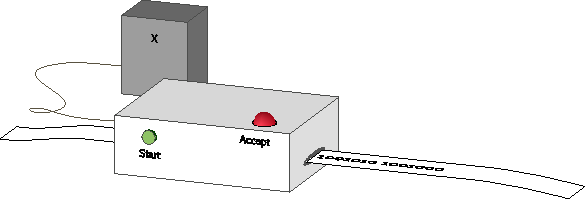
\includegraphics{asy/share/machine01.pdf}
\end{center}

我们可以通过扩展 Turing 机的定义，来形式化地定义
\definend{相对于预言机的计算（computation relative to an oracle）}\index{computation!relative to an oracle}\index{oracle!computation relative to}
$X\subseteq\N$。
不过，本节中底层细节的帮助不大，所以
\citetext{我们将在概念上描述它}{%
  完整的处理请见 \autocite{Rogers}.}。
想象一下，从一个编程语言出发，添加一个布尔函数 \codeinline{oracle?}，
或者允许流程图包含查询步骤。\footnote{%
  一次相对于预言机的特定计算，可能会使用一次这样的查询，或多次，或一次也不用。
  }


\begin{center}
\begin{minipage}{2.3in}
\begin{lstlisting}
(if (oracle? x)
    (displayln "It is in the set")
    (displayln "It is not in the set"))
\end{lstlisting}
\end{minipage}
\qquad
\vcenteredhbox{\includegraphics{\asydir flowcharts/flowcharts21.pdf}}
\end{center}


% If $x\in X$
% then this takes one branch, while if $x\notin X$ then it takes the other.

我们可以更换预言机而不改变程序代码：
在图中，如果我们换掉黑盒，把 $X$~预言机换成 $Y$~预言机，
那么白色的 CPU 盒保持不变。
当然，预言机查询返回的值可能会改变，
从而可能在我们运行这个双盒系统时改变纸带输出。
但这样的交换不会改变白色的硬件。

我们已有的关于 Turing 机的其他结论同样适用。
特别地，每一台这样的机器——每一个 CPU 盒——都有一个索引。
这个索引是源码等价的，意思是给定一个索引，我们可以计算出
机器的源代码，而给定源代码，我们可以找到索引。

因此，要完整地指定这样一个计算，我们必须同时指明
我们使用的是哪台机器以及哪个预言机。
这就解释了带预言机的 Turing 机的记号：
\definend{$\TM_e^X\!$}，\index{oracle Turing machine}\index{oracle!Turing machine}\index{Turing machine!with oracle}
以及相关函数的记号：
\definend{$\TMfcn^X_e\!$}。\index{computable function!relative to an oracle}

\begin{definition}  \label{def:TuringReducible}
设~$X$ 为一个集合。
如果集合~$S$ 的特征函数可由~$X$ 计算，
即存在某个~$e$ 使得 $\charfcn{S}=\TMfcn^X_e$，那么
我们称~$S$ 是
\definend{可由预言机~$X$ 计算的},\index{computable!from a set}\index{oracle!set computable from}
或称~$S$ 是
\definend{$X$-可计算的},\index{computable!relative to a set}
% or is
% \definend{computable relative to~$X$},\index{computable!relative to a set}
或说 $S$ \definend{归约到~$X$},\index{reducibility}\index{set!reducibility}
或称 $S$ 是
\definend{Turing 可归约到~$X$},\index{Turing reducibility}\index{T reducible@$T$ reducible|see{Turing reducibility}}
记作 \definend{$S\leq_T X$}。\footnotemark
\end{definition}

\footnotetext{%
  我们已经在第~\protect\pageref{pageref:reducesto}~页关于 \protect\HP{} 的讨论中指出，
  一个常见的错误是把 $S\leq_T X$ 读作“$X$ 归约到 $S$”，
  而正确的读法是“$S$ 归约到 $X$”。}

直观上，$X$ “知道”的至少和~$S$ 一样多
% behind $S\leq_T X$
% or is at least as general as~$S$,
或者说 $X$ 至少具有和~$S$ 一样多的计算内容，因为
关于~$X$ 的问题的回答足以给出关于~$S$ 的问题的回答。

% \begin{remark}
% Here we use the letter $X$ for a general oracle, but we use other letters for
% specific sets.
% Think of $X$ as connoting that the machine has a plug
% that is capable of accepting
% an oracle black box, while another letter means that we have attached
% a device.
% \end{remark}


\begin{example}  \label{ex:KLeqTHaltsOnThree}
回想判定给定~$e$ 时 $\TM_e$ 在输入~$3$ 上是否停机的问题。\index{Halts On Three problem@\probname{Halts On Three} problem}
该问题要求一台机器充当集合
$A=\set{e\suchthat \text{$\TM_e$ halts on~$3$}}$ 的特征函数。
我们将证明 $K\leq_T A$。

要构造预言机 $\TM_e^{X}\!$，
我们首先回顾 \zcref{ex:HaltOnThree}。
从下方左边的函数 $\map{\psi}{\N^2}{\N}$ 开始。
中间的流程图加上 Church 论题表明存在一台
Turing 机，其输入-输出行为是 $\psi$；设其索引为~$e_0$。
\smn{} 定理给出了
一个以 $x$ 为参数的机器族 $\TM_{s(e_0,x)}$，
如右边所示。
那么对于任意 $k\in\N$，$k\in K$ 当且仅当
$s(e_0,k)\in A$。
\begin{center}
  $\psi(x,y)=
  \begin{cases}
    42        &\case{if $\TMfcn_x(x)\converges$} \\
    \;\diverges &\case{otherwise}
  \end{cases}$
  \qquad
  \vcenteredhbox{\includegraphics{\asydir flowcharts/flowcharts1033.pdf}}
  \qquad
  \vcenteredhbox{\includegraphics{\asydir flowcharts/flowcharts1034.pdf}}
\end{center}

由此我们可以构造预言机。
下面图示的机器就是 $\TM_e^{X}\!$。
它使用了前一段中的~$e_0$。
如果我们将其连接到 $A$~预言机，
那么根据前一段的最后一句，它就能计算 $K$ 的特征函数。
\begin{center}
  \vcenteredhbox{\includegraphics{\asydir flowcharts/flowcharts22.pdf}}
\end{center}
\end{example}

\begin{example}
设 $B=\set{e\suchthat \text{$\TMfcn(y)=\TMfcn(y+1)$ for some $y$}}$。
我们将证明 $K$ 归约到~$B$，即 $K\leq_T B$。

我们可以重用前一个例子中的函数 $\psi(x,y)$。
如同那里，$\psi$ 是直观可计算的，所以
Church 论题断言存在一台 Turing 机，其行为就是~$\psi$。
设该机器的索引为~$e_0$。
再次应用 \smn~定理对~$x$ 进行参数化，
得到机器族 $\TMfcn_{s(e_0,x)}$。
注意 $k\in K$ 当且仅当 $s(e_0,k)\in B$。
由此，同样的预言机就表明 $K\leq_T B$。
\end{example}

\subsection{Turing 等价}
正如小于等于号 $\leq_T$ 所暗示的，
我们有一种序关系，其中某些集合排在其他集合之前。
% \footnote{%
%   This ordering between sets turns out not to be linear.
%   It is more
%   \protect\citetext{like the `divides' relation between integers}{%
%     This is not a partial order because $A\leq_T B$ and $B\leq_T A$\
%     does not imply that $A=B$.
%     Instead, this is called a `preorder'.},
%   where $2$ divides~$6$ and $2$ divides~$10$, but $6$ and $10$
%   are not related.}

\begin{theorem} \label{th:TReductionReflexiveAndTrans}
\begin{thmparts}
\item \textsc{（自反性）} 每个集合都可以由自身计算，即 $A\leq_T A$。
\item \textsc{（传递性）} 如果 $A\leq_T B$ 且 $B\leq_T C$，那么 $A\leq_T C$。
\end{thmparts}
\end{theorem}

\begin{proof}
对于自反性，我们必须说明如何用 $A$~预言机计算 $\charfcn{A}$。
给定一个数~$x$，我们必须使用 $A$ 预言机判定 $x\in A$。
这是平凡的，因为这些问题正是预言机所回答的。

对于传递性，假设 $\TM_e^B$ 计算了~$A$ 的特征函数，
并且 $\TM_{\hat{e}}^C$ 计算了~$B$ 的特征函数。
那么要从~$C$ 直接计算 $A$ 的特征函数，
只需从用 $B$ 计算 $A$ 的过程出发，将其中的
$B$-预言机调用替换为对 $\TM_{\hat{e}}^C\!$ 的调用。
\end{proof}

接下来我们证明，在此序的最开端存在一些集合。

\begin{lemma}
\label{lem:ComputableOracleDoesNothing}
如果集合~$Y\subseteq\N$ 是可计算的，那么它可以归约到任意集合，
即对任意~$X\subseteq\N$ 均有 $Y\leq_T X$。
进一步，$Y$ 是可计算的当且仅当它可以归约到某个可计算集合，
即存在可计算集合 $S$ 使得 $Y\leq_T S$。
特别地，一个集合是可计算的当且仅当它可以归约到 $\emptyset$。
\end{lemma}

\begin{proof}
假设~$Y$ 可计算，即其特征函数可计算。
那么该特征函数可相对于预言机~$X$ 计算，只需从不向预言机询问任何问题。

关于“进一步”，前一段已证明若 $Y$ 可计算，则它可归约到某个可计算的~$S$，因为它可归约到任意 $S$。
对于另一个方向，
假设~$Y$ 的特征函数可借助某个可计算预言机计算，
即 $\charfcn{Y}=\TMfcn_e^S$，其中 $\charfcn{S}$ 可计算。
那么将机器 $\TM_e^S$ 中的预言机调用替换为 $\charfcn{S}$ 的直接计算，
即可在不借助预言机的情况下计算出 $\charfcn{Y}$。
因此 $Y$ 可计算。
\end{proof}

\begin{definition}
两集合 $A,B$ 称为
\definend{Turing 等价},\index{Turing equivalent}\index{set!Turing equivalent}\index{T-equivalent@$T$-equivalent|see {Turing equivalent}}
记作 \definend{$A\equiv_T B$}，若 $A\leq_T B$ 且 $B\leq_T A$。
\end{definition}

\begin{example}
\zcref{lem:ComputableOracleDoesNothing} 表明任意两个可计算集合均 Turing 等价。
\end{example}

证明两集合 $T$-等价，即它们相互可计算，
揭示了二者间内在的统一性。
在某种意义上，它们是同一个问题。

\begin{example}
\zcref{ex:KLeqTHaltsOnThree} 证明 $K\leq_T A$，
其中 $A=\set{e\suchthat \text{$\TM_e$ halts on~$3$}}$。
\zcref{exer:THaltsOnThreeLeqK} 证明 $A\leq_T K$。
故 $A\equiv_T K$。
\end{example}

当然，\HP{} 问的是 $\TM_e$ 在输入~$e$ 上是否停机。
有人或许觉得更自然的问题是判定 $\TM_e$ 在输入~$x$ 上是否停机。

\begin{definition} \index{K0, set of halting pairs@$K_0$, set of halting pairs}
  $\definend{K_0}=\set{\sequence{e,x} \suchthat \text{$\TM_e$ halts on input~$x$}}$
\end{definition}

\begin{theorem}
集合 $K$ 与 $K_0$ Turing 等价，
即 $K\equiv_T K_0$。\footnotemark
\end{theorem}

\footnotetext{%
  因此选择~$K$ 作为我们的试金石只是出于方便与惯例。
  我们使用它是因为它具有一些技术优势，
  包括它源自我们在 \protect\HP{} 章节开头所做的对角化推演，
  并且因为它是文献中的标准。}

\begin{proof}
先证 $K\leq_T K_0$。假设我们可以访问 $K_0$-预言机。
则将下方机器连至此预言机，其输入/输出行为即为 $K$ 的特征函数。
\begin{center}
  \vcenteredhbox{\includegraphics{\asydir flowcharts/flowcharts23.pdf}}
\end{center}

再证 $K_0\leq_T K$。考虑下方的左侧流程图：
它对输入三元组 $\sequence{e,x,y}$ 停机当且仅当 $\sequence{e,x}\in K_0$。
由 Church 论题，存在 Turing 机实现之；设该机索引为~$e_0$。
\begin{center}
  \includegraphics{\asydir hp/hp03.pdf}
  \hspace*{4em}
  \includegraphics{\asydir hp/hp04.pdf}
\end{center}
应用 \smn{} 定理对 $e$ 和~$x$ 进行参数化，便得到右侧流程图。
也就是说，右侧是 $\TM_{s(e_0,e,x)}$ 的草图。

现在考虑预言机 Turing 机。
对于输入对 $\sequence{e,x}$，上右侧机器在所有输入~$y$ 上行为相同。
它要么在所有输入上均停机，
要么在所有输入上均不停机，这取决于是否有 $\phi_e(x)\converges$。
特别地，当且仅当 $\TMfcn_e(x)\converges$ 时，
$\TM_{s(e_0,e,x)}$ 在输入 $y=s(e_0,e,x)$ 上停机，从而 $s(e_0,e,x)\in K$。
\begin{center}
  \vcenteredhbox{\includegraphics{\asydir flowcharts/flowcharts24.pdf}}
\end{center}
因此，给定预言机~$K$，上述机器便充当了 $K_0$ 的特征函数。
\end{proof}

\begin{corollary}
\HP{} 至少与任何可计算枚举问题一样难：对所有~$e\in\N$，$W_e\leq_T K$。
\end{corollary}

\begin{proof}
可计算枚举集即 $K_0$ 的各列，因
$
  W_e
  =\set{y\suchthat \TMfcn_e(y)\converges}
  =\set{y\suchthat \sequence{e,y}\in K_0}
$。
因此从 $K_0$ 预言机计算 $W_e$ 是容易的，且有
$W_e\leq_T K_0\equiv_T K$。
\end{proof}

因为每个可计算枚举集均可由~$K$ Turing 计算，我们说 $K$ 在可计算枚举集中是
\definend{完备的}\index{complete}\index{computably enumerable!K is complete@$K$ is complete}\index{K, the Halting problem set@$K$, the Halting problem set!complete among computably enumerable sets}。

% ..........................................
\subsection{跳跃}
$\leq_T$ 序按照计算难度对集合进行排序。
这如图所示。
点表示集合 $S\subseteq\N$。
若 $S\leq_T X$，则将 $S$ 画在~$X$ 下方。
可计算集位于底部，与空集归为一组。
与 $K$ Turing 等价的集合聚成一组，位于可计算枚举集的顶部。

\begin{fig}{依 $\leq_T$ 排序的 $\N$ 子集。}
  \includegraphics{\asydir ordering/ordering000.pdf}
  \label{fig:SubsetsNRankedByTReduction}
\end{fig}

在本节结束前，我们描述一种方法：从一个集合~$S$ 出发，
然后\citetext{在阶上进一步跃升}{%
  这类似于基数的情况，取幂集会跳到一个更大的基数。}。
我们的典型例子是从 $\emptyset$ 出发，跃升到~$K$。

\begin{definition}
对任意集合~$S$，\definend{相对于 $S$ 的停机问题（\probname{Relativized Halting} problem for $S$）}
就是判定 $\definend{\smash{K^S}}=\set{x\suchthat \smash{\TMfcn_x^S}(x)\converges}$ 的成员资格。\index{Relativized Halting problem@\probname{Relativized Halting} problem}\index{Halting problem@\probname{Halting} problem!relativized to a set}\index{Relativized Halting problem set@\probname{Relativized Halting} problem set $K^S$}
\end{definition}

\begin{theorem}
每个集合~$S$ 都可归约到其\probname{相对停机问题}，即 $S\leq_T K^S\!$。
\end{theorem}

\begin{proof}
下面左边是一台直观上可由机械计算的预言机。
因此，由 Church 论题，它有一个索引，使得它是某个~$e_0$ 对应的 $\TM_{e_0}^X$。
利用 \smn{} 定理对~$x$ 进行参数化，便得到右侧所示
一致可计算的机器族 $\TM_{s(e_0,x)}^X$。
\begin{center}
\vcenteredhbox{\includegraphics{\asydir flowcharts/flowcharts04.pdf}}
\hspace{2.5em}
\vcenteredhbox{\includegraphics{\asydir flowcharts/flowcharts05.pdf}}
\end{center}
% The machine on the right halts for any input~$y$
% if and only if $x$ is a member of the oracle.
取预言机为~$S$，$y$ 取为 $s(e_0,x)$，则 $x\in S$
当且仅当 $\TMfcn_{s(e_0,x)}^S(s(e_0,x))\converges$，
当且仅当 $s(e_0,x)\in \smash{K^S}\!$。
因此，如果 $\smash{K^S}$ 作为下面这台机器的预言机
\begin{center}
\vcenteredhbox{\includegraphics{\asydir flowcharts/flowcharts25.pdf}}
\end{center}
那么该机器就可作为集合~$S$ 的特征函数。
\end{proof}

\begin{theorem}
对任何集合~$S$，$K^S$ 都不可归约到~$S$。
即，$K^S\not\leq_T S$。
\end{theorem}

\begin{proof}
假设相反，即存在相对于预言机 $S$ 的计算，它能作为 $K^S$ 的特征函数。\footnotemark{} %
令该机器的索引为~$e_0$。
\begin{equation*}
  \TM_{e_0}^S(x)=
  \charfcn{K^S}(x)=
  \begin{cases}
  1  &\case{if $\TMfcn^S_x(x)\converges$}  \\
  0  &\case{otherwise}
  \end{cases}
  \tag{$*$}
\end{equation*}
考虑下面的预言机。
（注意，其中的判断框使用了索引为~$e_0$ 的机器。）
由 Church 论题，此预言机有一个索引；记其为 $e_1$。
\begin{center}
\vcenteredhbox{\includegraphics{\asydir flowcharts/flowcharts03.pdf}}
\end{center}
将 $S$ 预言机接入此机器，
并考虑当 $x=e_1$ 时会发生什么。

根据 ($*$)，函数 $\TMfcn_{e_0}^S(x)$ 对所有~$x$ 都收敛。
如果在判断框中 $\TMfcn^S_{e_0}(e_1)=0$，
那么这台机器会停机，
而这便产生了矛盾，因为根据 ($*$)，计算 $\TM_{e_0}^S(e_1)$
仅在 $\TMfcn_{e_1}^S(e_1)$ 发散时输出~$0$。
如果 $\TMfcn^S_{e_0}(e_1)=1$，
那么这台机器永不停机，
这同样是一个矛盾，因为 ($*$) 指出
计算 $\TM_{e_0}^S(e_1)$ 仅在 $\TMfcn_{e_1}^S(e_1)$ 收敛时输出~$1$。
无论哪种情况，假设~($*$) 成立都会导出矛盾。
\end{proof}

\footnotetext{%
  这是将 \zcpageref{th:HPIsUnsolvable} 中关于 \protect\HP{}
  不可解的证明，适配到相对于预言机的计算上。
  这样的适配称为\protect\definend{相对化（relativization）}\protect\index{relativization}。}

\begin{corollary}
特别地，有 $K\leq_T K^K$ 但 $K^K\not\leq_T K$。
\end{corollary}

\begin{proof}
这可由前两个结论直接得出。
\end{proof}

本节开头曾问，是否存在比停机问题更难的问题。
我们现在有了答案：一个严格比计算 $K$ 的特征函数更难的问题是
计算 $K^K$ 的特征函数。

\begin{exercises}[回顾第~\pageref{def:ComputableFcn} 页：如果一台 Turing 机计算某个集合的特征函数，那么它就是该集合的判定器。]

\begin{exercise}
\begin{credit}
  \url{https://mathoverflow.net/questions/33046/arent-oracle-machines-unsound-concepts},
  （那里的问题及其阐述与此改编版本有所不同。）
\end{credit}
你该如何回答你的朋友？
“你可以将不可判定的问题（如停机问题）作为预言机。但是，
假设存在一台能够判定停机问题的机器……这难道不是有问题的吗？”
\begin{answer}\verified
% It depends on what ``assume the existence of'' means.
我们并不假定存在一个原则上物理可实现、能在有限时间内
正确回答“$\TM_e$ 在输入~$e$ 上是否停机？”这类问题的装置。
但在论证中使用这样的表述是没有问题的：“假设我们有一个停机问题预言机，那么我们就可以……”。

\textit{评论}。
值得提及的是，“预言机”这个概念，
无论是本节所描述的形式，还是其延伸形式——
例如能解决密码学问题的预言机、能在线性时间内对数字列表排序的预言机等，
在解决实际问题时都非常常用。
\end{answer}
\end{exercise}

% \recommended


\begin{exercise}
预言机和判定器都接受一个数并返回 $0$ 或~$1$，以此表明该数是否属于某个集合。
它们有什么区别？
\begin{answer}\verified
  判定器是一台 Turing 机，其计算出的函数是某个集合的特征函数。
  预言机本身是一个集合，作为 Turing 机的附加部分，供机器查询。
\end{answer}
\end{exercise}

\recommended


\begin{exercise}
\begin{credit}
  \href{https://cs.stackexchange.com/q/40605/67754}{SE user Karolis Juodel\.{e}}
\end{credit}
你的朋友对教授说：“预言机不是真实存在的，那为什么还要讨论它们？”
教授该如何回答？
\begin{answer}\verified
  首先，它们既有趣又引人入胜。
  % Is that not enough?
  除此之外，它们有助于我们理解问题之间的关系。
  这包括试图理解哪些问题容易、哪些问题困难。

  在复杂性章节中，我们将扩展这一思想，以帮助理解许多日常的、实际的问题是如何相互关联的。
\end{answer}
\end{exercise}

\begin{exercise}
你的同学说，他们用“一个用来解决不可解问题的集合”来回答测验中“定义预言机”这道题。
请温和地评论一下。
\begin{answer}\verified
  他们的回答抓住了我们考虑预言机计算的原因的精髓，但在两个方面有所欠缺。
  第一，我们可以使用一个可计算集合（例如空集）作为预言机。
  （尽管使用可计算预言机确实无法解决任何没有它就无法解决的问题。）

  第二点不足是，他们的回答完全没有提及机制。
  预言机集合本身并不解决问题。
  我们可能会非正式地这么说，但作为定义，我们应该说：
  我们让一台 Turing 机能够查询关于预言机成员资格的答案，
  然后该机器的输入–输出行为才是问题的解。
\end{answer}
\end{exercise}

\recommended


\begin{exercise}
是否存在适用于所有问题的预言机？
对于每个问题，是否存在一个预言机？
\begin{answer}\verified
  我们将第一个问题理解为：是否存在一个最强大的预言机，能够解决所有问题？
  答案是否定的。
  给定集合 $X\subseteq \N$，判定 $K^X$ 的成员资格（即相对于该预言机的停机问题）无法仅凭 $X$ 来解决。

  第二个问题是：给定集合 $S\subseteq N$，是否存在一个足以判定 $S$ 成员资格的预言机？
  答案是肯定的：预言机 $S$ 本身就可以。
\end{answer}
\end{exercise}

\begin{exercise}
\begin{credit}
  \href{https://cs.stackexchange.com/a/96806/67754}{SE user Noah Schweber}
\end{credit}
你班上的同学问：“预言机能解决不可解问题，对吧？
而且 $K^K$ 是不可解的。
所以像 $K$ 这样的预言机应该能解决它。”
请帮教授想一个回应。
\begin{answer}\verified
  每个预言机只能计算某些问题的答案。
  （存在可数多个 $\TM_e^X$，但 $\N$ 的子集有不可数多个。）
  因此，对于每个预言机集合，都存在它无法解决的问题。
  具体来说，它无法解决相对于该集合的停机问题。
\end{answer}
\end{exercise}

\begin{exercise}
你的学习伙伴坦言：“我不理解相对计算。
任何停机计算都只能包含有限步。
所以如果其中有预言机调用，那么调用也只能有有限次。
但有限集是可计算的，因此根据\zcref{lem:ComputableOracleDoesNothing}，该有限集可归约到任何集合。”
请帮他们一下。
\begin{answer}\verified
  在一个停机的预言机计算中，确实只有有限次对预言机的调用。
  但当计算的输入是 $0$ 时进行的调用，很可能与输入是 $1$ 时进行的调用不同。
\end{answer}
\end{exercise}

\begin{exercise}
在图~\ref{fig:SubsetsNRankedByTReduction} 中加入 $K^K\!$。
\begin{answer}
它在 $K$ 之上。
\begin{display}
  \includegraphics{\asydir ordering/ordering001.pdf}
\end{display}
\end{answer}
\end{exercise}

\recommended

\begin{exercise}
\begin{credit}
  \url{http://people.cs.aau.dk/~srba/courses/tutorials-CC-10/t5-sol.pdf}
\end{credit}
假设集合 $A$ Turing 可归约到集合 $B$。
以下命题哪些为真？
\begin{exparts*}
\item $A$ 的判定器可用于判定 $B$。
\item 如果 $A$ 是可计算的，那么 $B$ 也是可计算的。
\item 如果 $A$ 是不可计算的，那么 $B$ 也是不可计算的。
\end{exparts*}
\begin{answer}\verified
  回顾一下，“$A$ Turing 可归约到 $B$”的记号是 $A\leq_T B$。
  \begin{exparts}
  \item 此命题为假。
  例如，空集可归约到停机问题集，即 $\emptyset\leq_T K$，但虽然空集的判定器是平凡的，却不存在 $K$ 的可计算判定器。

  正确的陈述恰恰相反：如果 $A\leq_T B$，那么我们可以使用 $B$ 的判定器来判定元素是否属于集合 $A$。
  \item 假。
  同上一项，若 $A$ 是空集，则它是可计算的。此时 $\emptyset\leq_T K$，但 $K$ 是不可判定的。
  正确的说法恰好相反：如果 $B$ 是可判定的，那么 $A$ 也是可判定的。
  \item 真。
  如果 $A\leq_T B$，则存在某个索引 $e\in\N$，使得函数 $\TMfcn_e^B$ 是 $A$ 的特征函数，即 $\TMfcn_e^B=\charfcn{A}$。
  利用这个函数，如果我们能计算 $B$，那我们就能用它来计算 $A$。
  因此，如果 $A$ 是不可计算的，那么 $B$ 也必定是不可计算的。
  \end{exparts}
\end{answer}
\end{exercise}

\begin{exercise}
对于集合 $B\subseteq\N$，令 $2B=\set{2b\suchthat b\in B}$。
我们将证明 $B\equiv_T 2B$。
\begin{exparts}
\item
给出一个机器的流程图草图，使得该机器在拥有对预言机 $2B$ 的访问权限时，能够作为 $B$ 的特征函数。
也就是说，这台机器证明了 $B\leq_T 2B$。
\item
绘制一台机器的草图，使其在拥有对预言机 $B$ 的访问权限时，能够作为 $2B$ 的特征函数。
这台机器证明了 $2B\leq_T B$。
\end{exparts}
\begin{answer}\verified
参见 \figureref{fig:BIsEquivToTwoB}。
\begin{figure}\centering
  \vcenteredhbox{\includegraphics{\asydir flowcharts/flowcharts1045.pdf}}
  \hspace{4em}
  \vcenteredhbox{\includegraphics{\asydir flowcharts/flowcharts1044.pdf}}
  \caption{证明 $B\leq_T 2B$ 和 $2B\leq_T B$。}
  \label{fig:BIsEquivToTwoB}
\end{figure}
\begin{exparts}
\item
左侧的流程图很直观。
\item
对于右侧的流程图，注意如果输入 $x$ 是奇数，那么这台机器必须回答“否”，因为任何奇数都不可能是 $2B$ 的元素。
\end{exparts}
\end{answer}
\end{exercise}

% \begin{exercise}
% We can use oracles for things other than determining the characteristic
% functions of sets.
% Sketch a machine that, with access to the oracle
% $P=\set{p\in \N\suchthat \text{$p$ is prime}}$,
% will input a number and print out a list of the primes
% dividing that number.
% \begin{answer}
% See \figureref{fig:OracleSetOfPrimes}.
% \begin{figure}\centering
%   \vcenteredhbox{\includegraphics{\asydir flowcharts/flowcharts1046.pdf}}
%   \caption{Oracle machine that can use the set of primes to find all primes dividing the input.}
%   \label{fig:OracleSetOfPrimes}
% \end{figure}
% \end{answer}
% \end{exercise}

\recommended


\begin{exercise}  \label{exer:THaltsOnThreeLeqK}
令 $A=\set{x\suchthat \text{$\TM_x$ halts on~$3$}}$，
证明 $A\leq_T K$。
\hint~这台机器 $\TM_e$ 满足 $\TMfcn_{e}(e)\converges$
当且仅当 $\TMfcn_x(3)\converges$。
\begin{center}
  \includegraphics{\asydir flowcharts/flowcharts1057.pdf}
\end{center}
\begin{answer}\verified
从下面的函数 $\map{\psi}{\N}{\N}$ 开始。
\begin{equation*}
  \psi(x,y)=
  \begin{cases}
    \TM_x(3)     &\case{if $\TM_x(3)\converges$}  \\
    \;\diverges  &\case{otherwise}
  \end{cases}
  \hspace*{4em}
  \vcenteredhbox{\includegraphics{\asydir flowcharts/flowcharts1056.pdf}}
  \hspace*{4em}
  \vcenteredhbox{\includegraphics{\asydir flowcharts/flowcharts1057.pdf}}
\end{equation*}
由 Church 论题，第一个流程图表明 $\psi$ 是机械可计算的。
设其索引为 $e_0$。
应用 S-m-n 定理对 $x$ 进行参数化，得到右侧草图所示的机器，其索引为 $s(e_0,x)$。
这台机器的行为不依赖于其输入 $y$，因此 $\TMfcn_{s(e_0,x)}(s(e_0,x))\converges$ 当且仅当
$\TMfcn_x(3)\converges$。
因此，给定 $x$，我们可以利用 $K$ 预言机测试该机器，从而判断 $x\in A$。
\begin{display}
  \vcenteredhbox{\includegraphics{\asydir flowcharts/flowcharts1058.pdf}}
\end{display}
\end{answer}
\end{exercise}

\recommended


\begin{exercise}
集合
$S=\set{e\suchthat \text{$\TMfcn_e(3)\converges$ and $\TMfcn_e(4)\converges$}}$
是不可计算的。
概述一台预言机来证明 $S\leq_T K$。
\hint~模仿
\zcref{ex:KLeqTHaltsOnThree}。
\begin{answer}\verified
% Mimicking \zcref{ex:KLeqTHaltsOnThree}, we go in two steps.
% First,
图 \figureref{fig:HaltsOnThreeKOracle} 左侧
是一个程序的流程图草图。
由 Church 论题，存在一台 Turing 机可以计算它。
设该机器的索引为 $e_0$。
\begin{figure}\centering
  \vcenteredhbox{\includegraphics{\asydir flowcharts/flowcharts1047.pdf}}
  \hspace{4em}
  \vcenteredhbox{\includegraphics{\asydir flowcharts/flowcharts1048.pdf}}
  \hspace{4em}
  \vcenteredhbox{\includegraphics{\asydir flowcharts/flowcharts22.pdf}}
  \caption{集合 $\set{x\suchthat \text{$\TMfcn_x(3)\converges$ and $\TMfcn_x(4)\converges$}}$ Turing 可归约到 $K$。}
  \label{fig:HaltsOnThreeKOracle}
\end{figure}
应用 S-m-n 定理得到一族以 $x$ 为参数的机器。
其第 $x$ 个成员显示在中间。
显然，如果它对某个输入停机，那么它对所有输入都停机。
因此，$\TM_x$ 在输入 $3$ 和 $4$ 上停机当且仅当 $s(e_0,x)\in K$。
换言之，存在一个可计算函数 $x\mapsto s(e_0,x)$，使得 $x\in\set{e\suchthat \text{$\TMfcn_e(3)\converges$ and $\TMfcn_e(4)\converges$}}$
当且仅当 $s(e_0,x)\in K$。
所以 $\set{e\suchthat \text{$\TMfcn_e(3)\converges$ and $\TMfcn_e(4)\converges$}}\leq_T K$。

现在我们利用可计算函数 $x\mapsto s(e_0,x)$ 来构造那台预言机。
参见图中右侧的流程图。
\end{answer}
\end{exercise}

\recommended


\begin{exercise}
对于集合 $S=\set{e\suchthat \TMfcn_e(3)\converges}$，
证明 $S\leq_T K_0$。
\begin{answer}\verified
根据定义，
$K_0=\set{\sequence{e,x}\suchthat \TMfcn_e(x)\converges}$。
所以 $e\in S$ 当且仅当 $\sequence{e,3}\in K_0$。
\end{answer}
\end{exercise}

\recommended

\begin{exercise}
证明 $K\leq_T \set{e\suchthat \text{$\TMfcn_e(y)=2y$ for all input $y$}}$。
\begin{answer}\verified
令 $D=\set{e\suchthat  \text{$\TMfcn_e(y)=2y$ for all inputs~$y$}}$。
  考虑以下函数。
  \begin{equation*}
    \psi(x,y)=
    \begin{cases}
      2y         &\case{if $\TMfcn_x(x)\converges$}  \\
      \;\uparrow  &\case{otherwise}
    \end{cases}
  \end{equation*}
  \begin{figure}
    \centering
    \vcenteredhbox{\includegraphics{\asydir flowcharts/flowcharts1051.pdf}}
    \hspace{4em}
    \vcenteredhbox{\includegraphics{\asydir flowcharts/flowcharts1052.pdf}}
    \hspace{4em}
    \vcenteredhbox{\includegraphics{\asydir flowcharts/flowcharts22.pdf}}
    \caption{证明 $K\leq_T \set{e\suchthat \text{$\TMfcn_e(y)=2y$ for all input $y$}}$。}
    \label{fig:MachinesDoubler}
  \end{figure}%
  根据图 \figureref{fig:MachinesDoubler} 左侧的流程图，
  由 Church 论题可知，存在一台 Turing 机，其输入/输出行为为 $\psi$。
  令那台 Turing 机的索引为 $e_0$，于是有 $\TMfcn_{e_0}=\psi$。

  应用 S-m-n 定理，得到一族函数 $\TMfcn_{s(e_0,x)}$，如图中间部分所示。
  那么 $x\in K$ 当且仅当 $s(e_0,x)\in D$。
  图右侧是一台预言机，表明 $K\leq_T D$，如所求。
\end{answer}
\end{exercise}

\begin{exercise}
考虑集合
$\set{e\suchthat \text{$\TMfcn_e(j)=7$ for some $j$}}$。
\begin{exparts}
\item 使用 Rice 定理证明它是不可计算的。
\item 概述如何使用 $K$ 预言机来计算它。
\end{exparts}
\begin{answer}\verified
\begin{exparts}
\item 令
$\mathcal{I}=\set{e\suchthat \text{$\TMfcn_e(j)=7$ for some $j$}}$。
该集合非空，因为存在一个元素，它是对于所有输入都输出 $7$ 的 Turing 机的索引。
该集合不是整个 $\N$，因为存在一个不属于它的元素，它是在所有输入上都永远不停机的 Turing 机的索引。

要说明 $\mathcal{I}$ 是一个索引集，假设 $e\in\mathcal{I}$，
且 $\hat{e}$ 满足 $\TMfcn_e\samebehavior\TMfcn_{\hat{e}}$。
因为 $e\in\mathcal{I}$，所以存在一个输入 $j$ 使得 $\TMfcn_e(j)=7$。
由于 $\TMfcn_e\samebehavior\TMfcn_{\hat{e}}$，对于同一个 $j$，我们有
$\TMfcn_{\hat{e}}(j)=7$，因此 $\hat{e}\in\mathcal{I}$。
\item
% We use \zcref{ex:KLeqTHaltsOnThree} as a basis.
图 \figureref{fig:EverOutputsSevenOracle} 左侧
是一幅程序的流程图草图。
第二张图更详细地说明了“交错并行”的具体内容。
由 Church 论题，存在一台 Turing 机可以计算该流程图。
令该机器的索引为 $e_0$。
\begin{figure}\centering
  \vcenteredhbox{\includegraphics{\asydir flowcharts/flowcharts1035.pdf}}
  \qquad
  \vcenteredhbox{\includegraphics{\asydir flowcharts/flowcharts1037.pdf}}
  \qquad
  \vcenteredhbox{\includegraphics{\asydir flowcharts/flowcharts1036.pdf}}
  \caption{用 $K$ 预言机计算 $\set{x\suchthat \text{$\TMfcn_x(j)=7$ for some $j$}}$。}
  \label{fig:EverOutputsSevenOracle}
\end{figure}
应用 S-m-n 定理，得到一族以 $x$ 为参数的机器，如第三个流程图所示。
显然，它对所有输入 $y$ 都停机，当且仅当 $\TM_x$ 对某个输入输出了一个 $7$。
因此，$\TM_x$ 输出过 $7$ 当且仅当 $s(e_0,x)\in K$。
这意味着存在一个可计算函数 $x\mapsto s(e_0,x)$，使得
$x\in\set{e\suchthat \text{$\TMfcn_e(j)=7$ for some $j$}}$
当且仅当 $s(e_0,x)\in K$。

要说明 $\set{e\suchthat \text{$\TMfcn_e(j)=7$ for some $j$}}\leq_T K$，
考虑图 \figureref{fig:EverOutputsSevenOracleII} 中的预言机。
如果将 $K$ 预言机接入该机器，那么根据上一段所述，
它的行为就是 $\set{e\suchthat \text{$\TMfcn_e(j)=7$ for some $j$}}$ 的特征函数。
\begin{figure}\centering
  \vcenteredhbox{\includegraphics{\asydir flowcharts/flowcharts22.pdf}}
  \caption{从 $K$ 计算 $\set{e\suchthat \text{$\TMfcn_e(j)=7$ for some $j$}}$ 的预言机。}
  \label{fig:EverOutputsSevenOracleII}
\end{figure}
\end{exparts}
\end{answer}
\end{exercise}

\begin{exercise}
令
$S=\set{e\in\N\suchthat \text{$\TMfcn_e(3)\converges$ and $\TMfcn_{2e}(3)\converges$ and $\TMfcn_e(3)=\TMfcn_{2e}(3)$}}$。
证明 $S\leq_T K$。
\begin{answer}\verified
图 \figureref{fig:PeAndPTwoEGiveSameOnThree} 左侧
是一个计算的草图。
由 Church 论题，存在一台具有相同行为的 Turing 机。
令那台机器的索引为 $e_0$。
\begin{figure}\centering
  \vcenteredhbox{\includegraphics{\asydir flowcharts/flowcharts1038.pdf}}
  \quad
  \vcenteredhbox{\includegraphics{\asydir flowcharts/flowcharts1039.pdf}}
  \quad
  \vcenteredhbox{\includegraphics{\asydir flowcharts/flowcharts22.pdf}}
  \caption{集合 $\set{x\suchthat \TMfcn_x(3)\converges=\TMfcn_{2x}(3)\converges}$ 与 $K$ 是 $T$ 等价的。}
  \label{fig:PeAndPTwoEGiveSameOnThree}
\end{figure}
应用 S-m-n 定理，得到一族以 $x$ 为参数的机器，
其第 $x$ 个成员 $\TM_{s(e_0,x)}$ 显示在中间图中。
显然，它对所有输入 $y$ 都停机当且仅当 $x\in S$。
特别地，它对输入 $y=s(e_0,x)$ 停机当且仅当 $x\in S$。
因此 $s(e_0,x)\in K$ 当且仅当 $x\in S$。
由此容易看出，将 $K$ 预言机接入右侧的预言机，
就使其表现为 $S$ 的特征函数。
故而 $S\leq_T K$。
\end{answer}
\end{exercise}

\begin{exercise}
回顾一下，如果一个可计算函数 $\TMfcn$ 对所有的 $y\in\N$ 都有
$\TMfcn(y)\converges$，则称其为\definend{全（total）函数}。\index{total function}\index{function!total}
全体全函数的集合记为
$\text{Tot}$。\index{Tot@$\text{Tot}$, set of total computable functions}
证明 $K\leq_T\text{Tot}$。
\begin{answer}\verified
考虑图 \figureref{fig:KLeqTot} 左侧所勾勒的例程。
由 Church 论题，存在一台具有该行为的 Turing 机。
令其索引为 $e_0$。
\begin{figure}\centering
  \vcenteredhbox{\includegraphics{\asydir flowcharts/flowcharts1040.pdf}}
  \qquad
  \vcenteredhbox{\includegraphics{\asydir flowcharts/flowcharts1041.pdf}}
  \qquad
  \vcenteredhbox{\includegraphics{\asydir flowcharts/flowcharts22.pdf}}
  \caption{用 $\text{Tot}$ 预言机计算 $K$。}
  \label{fig:KLeqTot}
\end{figure}
应用 S-m-n 定理，得到一族机器 $\TM_{s(e_0,x)}$，如中间所示。
观察到
$x\in K$ 当且仅当 $s(e_0,x)\in\text{Tot}$。
右侧是一台预言机，
当我们接入 $\text{Tot}$ 预言机时，它的行为将是 $K$ 的特征函数。
因此 $K\leq_T \text{Tot}$。
\end{answer}
\end{exercise}

\begin{exercise}
如果存在一个可计算的全函数~$\TMfcn$，使得每当 $\TMfcn_x(y)\converges$ 时两者结果一致，$\TMfcn_x(y)=\TMfcn(y)$，则称可计算偏函数~$\TMfcn_x$ 是
\definend{可扩展的（extensible）}\index{extensible function}\index{function!extensible}。
所有可扩展函数构成的集合记作 $\text{Ext}$。\index{Ext@$\text{Ext}$, extensible functions}
\begin{exparts}
\item 证明以下函数不是 $\text{Ext}$ 的成员：若 $x\in K$，则 $\operatorname{steps}(x)$ 是使 $\TM_x$ 在输入~$x$ 上于第~$s$ 步或之前停机的最小步骤数~$s$；否则 $\operatorname{steps}(x)\diverges$。
\item
证明 $K\leq_T\text{Ext}$。
\end{exparts}
\begin{answer}\verified
\begin{exparts}
\item 反设函数 $\operatorname{steps}$ 有一个可计算的扩展~$g$，根据可扩展的定义，$g$ 必须是全函数。
那么我们可以通过在输入~$x$ 上运行 $\TM_x$ 最多 $g(x)$ 步来解决 \HP{}。
如果 $\TMfcn_x(x)$ 的计算届时仍未停机，它就永远不会停机。
\item
考虑 \figureref{fig:ExtLeqTot} 左侧草图所示的程序。
根据 Church 论题，存在具有该行为的 Turing 机。
设其索引为~$e_0$。
\begin{figure}\centering
  \vcenteredhbox{\includegraphics{\asydir flowcharts/flowcharts1042.pdf}}
  \qquad
  \vcenteredhbox{\includegraphics{\asydir flowcharts/flowcharts1043.pdf}}
  \qquad
  \vcenteredhbox{\includegraphics{\asydir flowcharts/flowcharts1049.pdf}}
  \caption{使用 $\text{Ext}$ 预言机计算 $K$。}
  \label{fig:ExtLeqTot}
\end{figure}
应用 \smn{} 定理对~$x$ 进行参数化，得到一族如中间图所示的程序，
$\TM_{s(e_0,x)}$。
如果 $x\notin K$，那么
$\TMfcn_{s(e_0,x)}(y)$ 对所有输入~$y$ 都无定义，且
该函数是 $\text{Ext}$ 的成员，因为显然可计算的常零函数就是它的一个扩展。
如果 $x\in K$，那么 $\TMfcn_{s(e_0,x)}(y)=\operatorname{steps}(y)$ 对所有
输入~$y$ 都成立，且由第一项可知它不是~$\text{Ext}$ 的成员。
因此，
$k\in K$ 当且仅当 $s(e_0,k)\notin\text{Ext}$。
右侧的预言机在连接 $\text{Ext}$ 预言后，
将充当~$K$ 的特征函数。
所以 $K\leq_T \text{Ext}$。
\end{exparts}
\end{answer}
\end{exercise}

\begin{exercise}
设 $A$ 和~$B$ 为集合。
证明：如果在预言机计算 $\TMfcn^A(x)$ 过程中被查询的所有 $q\in\N$ 都满足 $A(q)=B(q)$，
那么 $\TMfcn^B(x)$ 给出的结果与 $\TMfcn^A(x)$ 相同。
\begin{answer}\verified
计算过程将完全相同地进行，因此会得到相同的结果。
\end{answer}
\end{exercise}

\recommended


\begin{exercise}
证明对所有 $A\subseteq\N$，有 $A\leq_T \setcomp{A}$。
\begin{answer}\verified
预言机程序见 \figureref{fig:ALeqAComp}。
该机器在连接 $\setcomp{A}$ 预言后，将充当~$A$ 的特征函数。
\begin{figure}\centering
  \vcenteredhbox{\includegraphics{\asydir flowcharts/flowcharts1050.pdf}}
  \caption{从 $\setcomp{A}$ 预言机计算 $A$。}
  \label{fig:ALeqAComp}
\end{figure}
\end{answer}
\end{exercise}

\begin{exercise}
证明 $K\nleq_T\emptyset$。
\begin{answer}\verified
根据 \zcref{lem:ComputableOracleDoesNothing}，可归约到~$\emptyset$ 的集合都是可计算的。
但 $K$ 不是可计算的。
\end{answer}
\end{exercise}

\begin{exercise}
预言机的数量是可数的还是不可数的？
\begin{answer}\verified
任何 $\N$ 的子集都可以作为预言机，所以有不可数多个预言机。
\end{answer}
\end{exercise}

\begin{exercise}
固定一个预言机。
有多少集合可由该预言机计算？
\begin{answer}\verified
  只有可数多个程序可能包含 \codeinline{oracle} 调用。
  也就是说，只有可数多台带预言机的 Turing 机，由 $\TM_e^X\!$ 中的索引~$e$ 枚举。
\end{answer}
\end{exercise}

\begin{exercise}
设 $A$ 和~$B$ 为集合。
构造一个集合~$C$，使得 $A\leq_T C$ 且 $B\leq_T C$。
\begin{answer}\verified
一个例子是
  $C=\set{\cantor(0,a)\suchthat a\in A}
      \cup\set{\cantor(1,b)\suchthat b\in B}$。
  显然，从这个集合我们可以回答关于元素是否属于~$A$ 和~$B$ 的问题。
\end{answer}
\end{exercise}

\begin{exercise}
关系 $\leq_T$ 是集合之间的关系，因此我们自然会问它与集合运算如何交互。
\begin{exparts*}
\item $A\subseteq B$ 是否蕴含 $A\leq_T B$？
\item $A\leq_T A\cup B$ 是否成立？
\item $A\leq_T A\cap B$ 是否成立？
\item $A\leq_T \setcomp{A}$ 是否成立？
\end{exparts*}
\begin{answer}\verified
  \begin{exparts}
  \item 否。
    \HP{} 集~$K$ 是自然数集~$\N$ 的子集，
    但 $K\nleq_T\N$，因为 \HP{} 是不可解的。
  \item 否。
    \HP{} 集 $K$ 不 Turing 可归约到~$\N=K\cup\setcomp{K}\!$，
    但 $K\subseteq K\cup\setcomp{K}\!$。
  \item 否。
    \HP{} 集 $K$ 不 Turing 可归约到~$\emptyset$，
    但 $\emptyset=K\cap\setcomp{K}\!$。
  \item 是。
    我们可以写出这个使用预言机的程序：读取输入~$x$，
    如果它属于预言机集合则输出~$0$，否则输出~$1$。
  \end{exparts}
\end{answer}
\end{exercise}

\begin{exercise}
假设 $A\leq_T B$。
%  and suppose that an outline of the
% oracle computation looks like this.
% (This is not the general case.
% The actual machine might more than one test.
% Or, it might write a number of \str{1}'s and them conditionally erase
% all of them, or all but one of them.)
% \begin{center}
%   \includegraphics{\asydir flowcharts/flowcharts1053.pdf}
% \end{center}
判断下列各项是真还是假，并简述论证。
\begin{exparts*}
\item $\setcomp{A}\leq_TB$
\item $A\leq_T\setcomp{B}$
\item $\setcomp{A}\leq_T\setcomp{B}$
\end{exparts*}
\begin{answer}\verified
参考 \figureref{fig:ALeqBImplies}。
%The flowchart given in the question statement is on the left.
\begin{figure}\centering
  \vcenteredhbox{\includegraphics{\asydir flowcharts/flowcharts1054.pdf}}
  \qquad
  \vcenteredhbox{\includegraphics{\asydir flowcharts/flowcharts1055.pdf}}
  % \quad
  % \vcenteredhbox{\includegraphics{\asydir flowcharts/flowcharts1053.pdf}}
  \caption{与补集相关的预言机。}
  \label{fig:ALeqBImplies}
\end{figure}
\begin{exparts}
\item 真。
这在左侧的流程图中展示。
基本上，交换 ‘yes’ 和 ‘no’ 的输出即可。
\item 真。
这在中间的流程图中展示。
将所有如顶部那样的预言机调用替换为底部的调用
（唯一区别是交换了 ‘Y’ 和 ‘N’）。
\item 真。
结合前两项。
\end{exparts}
\end{answer}
\end{exercise}

\begin{exercise}
设 $A\subseteq\N$。
\begin{exparts*}
\item
给出集合是
\definend{相对于预言机可计算枚举的（computably enumerable in an oracle）}的定义。\index{computably enumerable!in an oracle}\index{oracle!computably enumerable in}
\item
证明对于所有集合~$A$，$\N$ 是相对于 $A$ 可计算枚举的。
\item
证明 $K^A$ 是相对于~$A$ 可计算枚举的。
\end{exparts*}
\begin{answer}\verified
  \begin{exparts}
  \item 自然的方法是相对化 \zcref{def:ComputablyEnumerable}，
    并定义：如果 $B$ 是某个 $A$-可计算函数的值域，则集合~$B$ 是
    \definend{相对于集合~$A$ 可计算枚举的（computably enumerable in the set~$A$）}。
    即，$B$ 相对于 $A$ 是 c.e.\@ 的，如果
    $B=\set{\TMfcn_e^A(x)\suchthat x\in\N}$ 对某个索引~$e$ 成立（该
    函数可能是偏函数）。
  \item 如 \zcref{lem:ComputableOracleDoesNothing} 所示，我们甚至不需要查询预言机就能输出~$\N$ 的元素。
    函数 $\TMfcn^A(x)=x$ 是可计算的，且永远不需要
    查询预言机。
  \item 交错并行。
    首先，运行 $\TM_0^A$ 在输入~$0$ 上的一步计算。
    然后，运行 $\TM_0^A$ 在输入~$0$ 上的第二步计算，
    以及 $\TM_1^A$ 在输入~$1$ 上的一步计算。
    接下来，运行 $\TM_0^A$ 在输入~$0$ 上的第三步计算，
    $\TM_1^A$ 在输入~$1$ 上的第二步计算，
    以及 $\TM_2^A$ 在输入~$2$ 上的一步计算。
    继续这种方式，随着时间的推移，其中一些计算将会停机。
    当计算 $\TM_e^A(e)$ 停机时，将索引~$e$ 枚举入 $K^A\!$。
    （因此在枚举函数中，$\TMfcn^A(i)$ 是以这种方式
    列出的第 $i$ 个索引。）
  % \item
  % Hint: use $\emptyset$, $K$, and $\setcomp{K}$.
  \end{exparts}
\end{answer}
\end{exercise}

% Instead, define re in A, and prove that if S is re in A and S comp
% is re in A then S is recursive in A?

% \begin{exercise}
% Prove that
%   $\text{Tot}=\set{e\suchthat \text{$\TMfcn_e(y)\converges$ for all $y$}}$
% is $T$-equivalent to $K^K$.
% \end{exercise}

\end{exercises}
\index{oracle|)}\index{set!oracle|)}

% =====================================================
\section{不动点定理}\index{Fixed point theorem|(}

我们第一次遇到对角化\index{diagonalization}
是在证明实数集不可数时，见第~\pageref{th:RealsNotCountable}页。
%<*discussion:RecallCantorThm>
我们假设存在一个满射函数 $\map{f}{\N}{\R}$，
并考虑其输入和输出，如表所示。
\begin{equation*} \setlength{\arraycolsep}{0.75\arraycolsep}
  \begin{array}{c|r@{\hspace*{.35em}.\hspace*{.35em}}ccccccc@{\hspace*{1em}\ldots\;}}
    \multicolumn{1}{c}{\text{\small $n$\hspace*{0.25em}}}
    &\multicolumn{8}{c}{\text{\hspace*{-1.00em}\small\tabulartext{$f(n)$的小数展开}}}  \\
   \cline{1-9}
   \rule{0em}{2.15ex}% bit more vertical room
   0  &42  &3  &1  &2  &7  &7  &0  &4  \\
   1  &2   &0  &1  &0  &0  &0  &0  &0  \\
   2  &1   &4  &1  &4  &1  &5  &9  &2  \\
   3  &-20  &9  &1  &9  &5  &9  &1  &9  \\
   % 4  &  0 &1  &0  &1  &0  &0  &1  &0  \\
   % 5  &-0  &6   &2  &5  &5  &4  &1  &8  \\[-.5ex]
   \multicolumn{1}{c}{\vdotswithin{$0$}}
    &\multicolumn{4}{c}{\vdotswithin{$1$}}
  \end{array}
\end{equation*}
% Let row~$n$'s decimal representation be
% $d_n=\hat{d}_n.d_{n,0}\mskip 1mu d_{n,1}\mskip 1mu d_{n,2}\ldots$\sentencespace %
我们沿着小数点右侧的对角线得到数字序列 $d_{0,0}, d_{1,1}, d_{2,2}, \ldots$，
在上面的图示中为 $3,1,4,5,\ldots$\sentencespace
利用这一点，
我们构造了一个数~$z=0.z_0\mskip 1mu z_1\mskip 1mu z_2\ldots$，
使其第 $n$ 位小数 $z_n$ 不同于~$d_{n,n}$。
具体来说，我们采用数字变换~$t$，
当 $d_{n,n}=1$ 时由 $t(d_{n,n})=2$ 给出，否则由 $t(d_{n,n})=1$ 给出，
从而由上表得到 $z=0.1211\ldots$\sentencespace
然后我们的论证最终确认了~$z$
不是任何一行。
我们说我们通过从行的列表中“对角化出来”得到了 $z$。
%</discussion:RecallCantorThm>

\subsection{当对角化失败时}\index{diagonalization}
%<*discussion:WhenDiagonalizationFails>
如果变换使得对角线恰好是某一行，
即 $z=f(n_0)$，会怎样？
那么对角线与该行交叉处的数组元素在变换后不变，
即 $d_{n_0,n_0}=t(d_{n_0,n_0})$。
结论：如果对角化失败，那么变换有一个不动点。
%</discussion:WhenDiagonalizationFails>

%<*discussion:WhenDiagonalizationFailsi>
我们将把这一思想应用到可计算函数序列上，
$\TMfcn_{i_0},\TMfcn_{i_1},\TMfcn_{i_2} \ldots$\sentencespace
我们关心有效性，因此我们
% don't consider arbitrary sequences but instead
取索引
$i_0,i_1,i_2\ldots$ 为可计算的，即对于某个~$e$，有
$i_0=\TMfcn_e(0)$、$i_1=\TMfcn_e(1)$、$i_2=\TMfcn_e(2)$ 等。
简而言之，可计算函数的可计算序列具有这种形式。
\begin{equation*}
  \TMfcn_{\phi_e(0)},\;\TMfcn_{\phi_e(1)},\;\TMfcn_{\phi_e(2)}\;\ldots
\end{equation*}
%</discussion:WhenDiagonalizationFailsi>
%<*discussion:WhenDiagonalizationFailsii>
下面是所有此类序列的表。
%</discussion:WhenDiagonalizationFailsii>
%<*discussion:WhenDiagonalizationFailsiii>
\begin{equation*}\small \renewcommand{\arraystretch}{1.25}
  \begin{tabular}{rr|ccccc}
    &\multicolumn{1}{c}{\ }
    &\multicolumn{4}{c}{\tabulartext{Sequence term}}  \\
    &\multicolumn{1}{c}{\ }
      &$n=0$ &$n=1$ &$n=2$ &$n=3$ &\ldots \\  \cline{3-7}
   \multirow{5}{*}{\tabulartext{Sequence}}
    &$e=0$ &$\phi_{\phi_0(0)}$ &$\phi_{\phi_0(1)}$ &$\phi_{\phi_0(2)}$ &$\phi_{\phi_0(3)}$  &\ldots \\
    &$e=1$ &$\phi_{\phi_1(0)}$ &$\phi_{\phi_1(1)}$ &$\phi_{\phi_1(2)}$ &$\phi_{\phi_1(3)}$  &\ldots \\
    &$e=2$ &$\phi_{\phi_2(0)}$ &$\phi_{\phi_2(1)}$ &$\phi_{\phi_2(2)}$ &$\phi_{\phi_2(3)}$  &\ldots \\
    &$e=3$ &$\phi_{\phi_3(0)}$ &$\phi_{\phi_3(1)}$ &$\phi_{\phi_3(2)}$ &$\phi_{\phi_3(3)}$  &    \\[-.5ex]
    &\multicolumn{1}{c}{$\mathrel{\makebox[\widthof{$e=3$}]{\vdots}}$}
      &\multicolumn{1}{c}{$\mathrel{\makebox[\widthof{=}]{\vdots}}$}
      &$\mathrel{\makebox[\widthof{=}]{\vdots}}$
  \end{tabular}
  \tag{$*$}
\end{equation*}
%</discussion:WhenDiagonalizationFailsiii>
%<*discussion:WhenDiagonalizationFailsiv>
每个表项 $\TMfcn_{\TMfcn_e(n)}$ 都是一个可计算函数。
如果索引 $\TMfcn_e(n)$ 发散，则整个函数发散。
%</discussion:WhenDiagonalizationFailsiv>

%<*discussion:WhenDiagonalizationFailsv>
至于变换，对于可计算函数~$f\!$，自然的变换是这样的：
\begin{equation*}
  \TMfcn_x\mapsunder{t_f}\TMfcn_{f(x)}
  \qquad
  \text{使得 }
  \qquad
  \TMfcn_{\TMfcn_i(j)}\mapsunder{t_f}\TMfcn_{f(\TMfcn_i(j))}
\end{equation*}
接下来我们证明，在这个变换下，
对角化会失效。
因此~$t_f$ 有一个不动点。
%</discussion:WhenDiagonalizationFailsv>

\begin{theorem}[不动点定理，Kleene 1938]\hspace*{-0.5em}\footnotemark[1]  \label{th:FixedPointThm}
%<*th:FixedPointThm>
\index{Fixed Point theorem}\index{Kleene's Fixed Point theorem}\index{Recursion theorem}
\hspace*{-0.5em}对于任意全可计算函数~$f$，
存在一个数~$k$ 使得 $\TMfcn_k=\TMfcn_{f(k)}$。
%</th:FixedPointThm>
\end{theorem}

\footnotetext[1]{%
  这也称为递归定理。
  % But there is another widely used result with that name, and
  % this name is both common and more descriptive of the result.
}


\begin{proof}
%<*pf:FixedPointThmi>
下面的左侧流程图勾勒了一个函数
$f(n,x)=\TMfcn_{\TMfcn_n(n)}(x)$。
根据 Church 论题，必有某个 Turing 机计算此函数；设该
机器的索引为~$e_0$。
应用 s-m-n 定理对~$n$ 进行参数化，得到右侧流程图，
它描述了一族
机器。
该族的第~$n$ 个成员，$\TMfcn_{s(e_0,n)}$，
计算上面表~($*$) 对角线上的第~$n$ 个函数，
$\TMfcn_{\TMfcn_n(n)}$。
%</pf:FixedPointThmi>
\begin{equation*}
  \vcenteredhbox{\includegraphics{\asydir flowcharts/flowcharts06.pdf}}
  \hspace{2em}
  \vcenteredhbox{\includegraphics{\asydir flowcharts/flowcharts07.pdf}}
  \hspace{1em}
  \TMfcn_{s(e_0,n)}(x)=
  \begin{cases}
    \TMfcn_{\TMfcn_n(n)}(x)  &\case{if $\TMfcn_n(n)\converges$} \\
    \uparrow                &\case{otherwise}
  \end{cases}
\end{equation*}
%<*pf:FixedPointThmii>
索引~$e_0$ 是固定的，所以 $s(e_0,n)$ 是一个单变量函数。
令 $g(n)=s(e_0,n)$，使得对角线上的函数为
$\TMfcn_{\TMfcn_0(0)}=\TMfcn_{g(0)}$、$\TMfcn_{\TMfcn_1(1)}=\TMfcn_{g(1)}$、
\ldots\sentencespace
函数 $g$ 是可计算且全的，因为 $s$ 是可计算且全的。

在变换~$t_f$ 下，这些函数被变换为
$\TMfcn_{f\!g(0)},\,\TMfcn_{f\!g(1)},\,\TMfcn_{f\!g(2)},\,\ldots$\sentencespace
复合 $\composed{f}{g}$ 是可计算且全的，因为
$f$ 在定理陈述中被指定为可计算且全的。
%</pf:FixedPointThmii>
\begin{equation*}
  \TMfcn_{fg(n)}\,(x)=
  \begin{cases}
    \TMfcn_{f\TMfcn_n(n)}(x)   &\case{if $\TMfcn_n(n)\converges$}     \\
    \uparrow                 &\case{otherwise}
  \end{cases}
  \hspace{2.5em}
  \vcenteredhbox{\includegraphics{\asydir flowcharts/flowcharts08.pdf}}
\end{equation*}
%<*pf:FixedPointThmiii>%
正如流程图所强调的，
$\TMfcn_{f\!g(0)},\,\TMfcn_{f\!g(1)},\,\TMfcn_{f\!g(2)},\>\ldots\>$
是一个可计算函数的可计算序列。
因此它是表~($*$) 中的一行。
设该行为第~$v$ 行，使得对所有~$m$ 有 $\TMfcn_{f\!g(m)}=\TMfcn_{\TMfcn_{v}(m)}$。
考虑对角线序列 $\TMfcn_{\TMfcn_n(n)}=\TMfcn_{g(n)}$
与该行的交点：
% \begin{equation*}
  $\TMfcn_{g(v)}=\TMfcn_{\TMfcn_v(v)}=\TMfcn_{f\!g(v)}$。
% \end{equation*}
$f$ 的不动点是 $k=g(v)$。
%</pf:FixedPointThmiii>
\end{proof}

不动点定理说明，当我们试图对偏可计算函数进行对角化时，对角化
失效。
也就是说，
\citetext{偏可计算函数的概念似乎天生就有一种抵御对角化的机制}{%
  \autocite{Odifreddi}，第~152 页。}。

不动点定理
适用于任何全可计算函数。
因此它引出了许多结论，其中许多令人惊讶。

%<*cor:SuccessorFcnSame>


\begin{corollary}
存在一个索引~$e$ 使得 $\TMfcn_e=\TMfcn_{e+1}$。
\end{corollary}

\begin{proof}
函数~$f(x)=x+1$ 是可计算且全的。
所以存在 $e\in\N$ 使得 $\TMfcn_{e}=\TMfcn_{f(e)}$。
\end{proof}


%</cor:SuccessorFcnSame>

%<*cor:WeEqualsSete>


\begin{corollary} \label{cor:ExistsPhiNWithRanN}
存在一个索引~$e$ 使得 $\TM_e$ 仅在 $e$ 上停机。
\end{corollary}


%</cor:WeEqualsSete>

\begin{proof}
%<*pf:WeEqualsSetei>
考虑下面左侧流程图描述的机器。
根据 Church 论题，它可以用 Turing 机实现，
记为 $\TM_{e_0}$。
进行参数化得到右侧流程图，
$\TM_{s(e_0,x)}$。
%</pf:WeEqualsSetei>
\begin{equation*}
  \vcenteredhbox{\includegraphics{\asydir flowcharts/flowcharts09.pdf}}
  \hspace{1em}
  \vcenteredhbox{\includegraphics{\asydir flowcharts/flowcharts10.pdf}}
  \hspace{1em}
  \TMfcn_{s(e_o,m)}(x)=
  \begin{cases}
  42         &\case{if $x=m$}  \\
  \uparrow  &\case{otherwise}
  \end{cases}
\end{equation*}%
%<*pf:WeEqualsSeteii>
由于 $e_0$ 是固定的，
$s(e_0,m)$ 是一个单变量的全可计算函数，
$f(m)=s(e_0,m)$，其中
对应的 Turing 机仅在输入~$m$ 上停机。
函数~$f$ 有一个不动点，$\TMfcn_{f(e)}=\TMfcn_e$，
且对应的 Turing 机 $\TM_e$ 仅在~$e$ 上停机。
%</pf:WeEqualsSeteii>
\end{proof}

我们之前非正式地将机器的索引称为它的“名字”。
若用修辞的手法重述，这一结果说明：
\citetext{机器的名字就是它的行为方式}{%
  一个人或许不会惊讶于发现自己的朋友
  “波士顿的乔”出生在波士顿，但如果一个朋友在出生时起名叫
  “2038年1月19日彩票赢家史密斯”，然后他真的中了奖，这肯定会
  令人大跌眼镜。
  \definend{姓名决定论}
  是一种认为一个人的名字会对其一生的作为
  产生某种影响的理论。
  例子有：短跑运动员尤塞恩·博尔特，
  美国气象预报员斯托姆·菲尔兹，
  棒球运动员普林斯·菲尔德，
  以及名为 Igor Judge（我审判）的英格兰和威尔士首席大法官，
  I~Judge。
  参见 \url{https://en.wikipedia.org/wiki/Nominative_determinism}。}。
% \footnote{%
%   The use of `name' for `index'
%   is meant to be evocative.}

\begin{corollary}
存在 $m\in\N$ 使得
$\TMfcn_m(x)=m$ 对所有~$x$ 成立。
\end{corollary}

\begin{proof}
考虑函数 $\psi(x,y)=x$。
如下面左侧流程图所示，它是可计算的。
% \footnote{%
%   The flowchart is overkill here since the function
%   is obviously computable.
%   But when it is not obvious, as in
%   some exercises, we need an outline of how to compute the function.}
根据 Church 论题，存在一台 Turing 机计算它。
设该机器的索引为~$e_0$，因此 $\psi(x,y)=\TMfcn_{e_0}(x,y)=x$。
\begin{center}
  \vcenteredhbox{\includegraphics{\asydir flowcharts/flowcharts17.pdf}}
  \hspace*{2.5em}
  \vcenteredhbox{\includegraphics{\asydir flowcharts/flowcharts18.pdf}}
\end{center}
应用 s-m-n 定理得到一个
由~$x$ 参数化的一致可计算函数族，
由 $\TMfcn_{s(e_0,x)}(y)=x$ 给出。
令 $\map{f}{\N}{\N}$ 为 $f(x)=s(e_0,x)$。
因为~$e_0$ 是固定的，这是一个单输入的全可计算函数。
因此存在不动点~$m\in\N$ 使得
对所有~$y$ 有 $\TMfcn_m(y)=\TMfcn_{f(m)}(y)=\TMfcn_{s(e_0,m)}(y)=m$。
\end{proof}

同样，这台机器的行为与其索引相同。
假设我们查看了 $\TM_7$ 的源代码，发现它在所有输入上都输出~$7$。
我们或许会认为，这仅仅是我们为 Turing 机选择的编号方案所造成的一个离奇巧合。
但推论指出，任何可接受的编号方案都必然对某台机器存在这种索引与行为的巧合。

再者，由于 Turing 机的索引等价于源代码，这一结果暗示着存在一个能输出自身源代码、能自我复制的程序。
这是一种自我指涉；更多内容请参见 \zcref{sec:SelfReproduction}。

% ...........
\subsection{讨论}\index{Fixed point theorem!discussion|(}
不动点定理及其证明常被\citetext{认为是神秘莫测的，或至少是晦涩难懂的}{%
  例如，“递归定理……拥有最令人费解的证明之一，我无法解释它为何有效，只知道它确实有效。” \autocite{blog:ComputationalComplexityRecursionThm}}。
这里我们将围绕命名在这一定理中的作用阐述一个观点。

比较句子 \textit{Atlantis is a mythical city} （亚特兰蒂斯是一座神话城市）与
\textit{There are two t's in ‘Atlantis’} （“Atlantis” 这个词里有两个 t）。
在第一个句子里，我们说 ‘Atlantis’ 是\definend{被使用（used）}的，因为它指向某物，它具有一个值，它命名了某物。
在第二个句子里，‘Atlantis’ 并非在指称某物\Dash 它的值就是它自身\Dash 因此\citetext{我们说它是\definend{被提及（mentioned）}的}{%
  我们可以用使用—提及之分玩出很多花样。
  一个例子是那个古老的俏皮话：当有人说“没有东西和 orange 押韵”时，回答“不，它不押韵”，这里就利用了 nothing（没有东西）和 ‘nothing’（“没什么”这个词）之间的区别。
  另一个谜题是：我们都同意 $1/2=3/6$，但一个式子里面有个 $3$ 而另一个却没有\Dash 不同的东西怎么可能是相等的？
  解决方法当然是，断言它们相等是指它们所代表的数字相等，而非表示法本身。
  也就是说，在被提及的层面，‘$1/2$’ 和 ‘$3/6$’ 是不同的串；但在被使用的层面，它们指向同一个数字。}。\footnote{%
  这个区分在编程书籍中很常见。
  在句子“玩家人数是 \texttt{players}”中，第一个 ‘players’ 指人，而第二个是一个程序变量。
  打字机字体有助于区分。
  类似地，本书中用斜体表示有值的变量，如~$a$，
  用打字机字体表示作为值的字符，如~\protect\str{a}。}
这就是\definend{使用—提及之分（use-mention distinction）}，~\index{use-mention distinction}
即我们在两个不同层面上使用一个词。

计算机编程中也有类似的情况。
请看下面的 C 语言代码片段。
其中，\codeinline{x} 和 \codeinline{y} 是变量。
如果它们是普通变量，那么编译器会将它们与某个特定的内存单元关联起来。
例如，如果一个普通变量~\codeinline{a} 与单元~$122$ 关联，那么语句 \codeinline{a = 5} 将导致数值~$5$ 被存储在那个单元中。
这是该单元的一个名称。

\ifbool{MakingPaperCopy}{%
  \relax
}{%
\margingraphic{0.29\textwidth}{background/pix/xkcdpointers.png}{\label{fig:xkcdpointers}\href{https://xkcd.com/138/}{图片源自 \url{xkcd.com}}}
}
但第二行的星号意味着 \codeinline{x} 和~\codeinline{y} 不是普通变量，它们是
\definend{指针（pointer）}，它们与一个单元关联，但具有一些额外的含义。\index{pointer, in C}
四个垂直的图示通过展示机器内存单元随时间的变化来说明这一点。
假设编译器将~\codeinline{x}
与单元~$123$ 关联，将~\codeinline{y} 与~$124$ 关联。
第一个图示显示，单元~$123$ 中恰好存放着数字~$901$，
单元~$124$ 中存放着~$902$。

因为这些都是指针，
我们已经向编译器声明，我们感兴趣的是它们所指向的内存单元的内容：单元~$123$ 本身就是位置~$901$ 的名称，
而 $124$ 命名了位置~$902$。
第二个垂直图示展示了执行 \codeinline{*x = 42} 语句的效果。
系统并不会把 $42$ 放进 $123$，
而是把 $42$ 放进了 $901$。
% \footnote{%
%   Using the \,\codeinline{*} operator to access the value stored at a pointer
%   is called dereferencing that pointer.
%   % There is a matching referencing operator, \codeinline{&},
%   % that gives the address of an existing variable.
%   % Both allow a programmer to control the indirection that pointers provide.
%   }
接着，通过 \codeinline{y = x}，系统将 \codeinline{y} 所指名的单元设置为指向与~\codeinline{x} 的单元相同的地址，即地址~$901$。
最后，最后一行代码将 $13$ 放入 \codeinline{y} 所指向的位置，此时也就是~\codeinline{x} 所指向的同一个单元。
\ifbool{MakingPaperCopy}{%


\begin{fig}{一个 C 程序中的指针。}
    \includegraphics{\asydir memory/memory04}
  \end{fig}


}{%

\begin{animatedfigure}{C 程序中的指针。}
  \vcenteredhbox{\animategraphics[poster=last]{1}{\asydir memory/memory}{00}{04}}
  \end{animatedfigure}


}

在这里，与 `Atlantis` 一样，\codeinline{x} 和~\codeinline{y} 在两个不同的层次上被使用。
一层是，\codeinline{x} 指代寄存器 $123$ 中的内容，因此它命名了~$123$。
另一层是，系统被设置成指代“内容的内容”，即地址~$901$ 中的内容。
在这一层上，\codeinline{x} 和~\codeinline{y} 就是名称的名称。

至于名称在不动点定理中扮演的角色，
回顾填充引理，\zcref{lem:EveryCompFcnHasInfManyIndices}，
即每个可计算函数都有无限多个索引。
因此，一个可计算函数很容易有两个不同的名称。
我们在 \zcref{th:FixedPointThm} 中看到了这一点，定理的结论 $\TMfcn_k=\TMfcn_{f(k)}$ 并没有说那两个索引
是相等的。
它说的是，它们描述了两台产生相同输入/输出关系的机器。

另一个例子是证明中的 $g(n)$：\begin{equation*}
  \TMfcn_{g(n)}(x)=
  \TMfcn_{s(e_0,n)}(x)=
  \begin{cases}
    \TMfcn_{\TMfcn_n(n)}(x)  &\case{if $\TMfcn_n(n)\converges$}  \\
    \uparrow                &\case{otherwise}
  \end{cases}
  \tag{$*$}
\end{equation*}。
所以 $g(n)$、$s(e_0,n)$ 和 $\TMfcn_n(n)$ 是同一个函数的名称。
同样地，被命名的函数相等并不意味着名称本身相等。

% Instead, $g(n)$ is an index of what is sketched in the right-hand of the
% pair of flowcharts in the proof.
% It is a name for a procedure that computes the function above.
非正式地说，$g(n)$ 命名的是这样一个过程：
“给定输入~$x$，在输入~$n$ 上运行 $\TM_n$，如果它停机并输出~$w$，那么就在输入~$x$ 上运行 $\TM_w$。”
更简短的说法是：“产生 $\TMfcn_n(n)$，然后执行 $\TMfcn_n(n)$。”
所以这里我们也看到了使用—提及之分。

被命名之物与名称本身之间的区分之所以重要，一个体现是：
无论 $\TMfcn_n(n)$ 是否收敛，
我们仍然可以计算出索引~$g(n)$，并由此得到指令集 $\TM_{g(n)}$。
这里可以拿 `Atlantis` 做个类比\Dash 尽管所指的城市并不存在，我们
仍然可以有意义地断言关于其名称的事情。
\index{Fixed point theorem!discussion|)}

\medskip
总而言之，不动点定理是深刻的，它揭示了在任何足够强大的计算系统中，
都会出现令人惊讶且有趣的行为。

% ................................................
\begin{exercises}


\begin{exercise}
你的朋友问起不动点定理的证明，
\zcref{th:FixedPointThm}。
“最后一行说 $\TMfcn_{g(v)}=\TMfcn_{\TMfcn_v(v)}$；这难道不就是在说 $g(v)=\TMfcn_v(v)$ 吗？
为什么要拐弯抹角呢？”
你怎么回答？
\begin{answer}\verified
  在日常编程中，我们很容易写出两段不同的源代码，
  它们却具有相同的输入/输出行为，即计算的是同一个函数。
  类似地，说这两者计算同一个函数，即 $\TMfcn_{g(v)}=\TMfcn_{\TMfcn_v(v)}$，
  与说它们由同一台 Turing 机产生（即索引相同）是两回事。
\end{answer}
\end{exercise}

\recommended


\begin{exercise}
证明以下各条。
\begin{exparts*}
\item 存在一个索引~$e$，使得 $\TMfcn_e=\TMfcn_{e+7}$。
\item 存在一个~$e$，使得 $\TMfcn_e=\TMfcn_{2e}$。
\end{exparts*}
\begin{answer}\verified
  \begin{exparts}
  \item 将不动点定理应用于全可计算函数 $f(x)=x+7$。
  \item 将不动点定理应用于全可计算函数~$f(x)=2x$。
  \end{exparts}
\end{answer}
\end{exercise}

\begin{exercise}
将不动点定理应用于加五函数 $x\mapsto x+5$，你能得出什么结论？
推广这个结论。
\begin{answer}\verified
  无论我们使用什么样的编号方案（只要它是可接受的），
  总存在一台 Turing 机，它计算的函数与索引比它大~5 的那台机器相同，
  也就是说，存在某个 $k\in\N$ 使得 $\TMfcn_k=\TMfcn_{k+5}$。

  自然的推广是：对于任何可接受的编号方案以及任何常数~$c\in\N$，
  都存在一台 Turing 机，它计算的函数与索引比它大~$c$ 的那台机器相同。
  即存在一个 $k\in\N$，使得 $\TMfcn_k=\TMfcn_{k+c}$。
\end{answer}
\end{exercise}

\begin{exercise}
通过对下列每个函数应用不动点定理，关于 Turing 机的可接受枚举，你能得出什么结论？
\begin{exparts*}
\item 三倍函数 $x\mapsto 3x$。
\item 平方函数 $x\mapsto x^2\!$。
\item 除了在 $x=5$ 时输出 $1$ 外，其余情况均输出 $0$ 的函数。
\item 常值函数 $x\mapsto 42$。
\end{exparts*}
\begin{answer}\verified
  \begin{exparts}
  \item 对于任何（可接受的）Turing 机编号方案，都存在一台机器，其计算的函数与索引为其三倍的那台机器相同。
    即，存在 $k\in\N$ 使得 $\TMfcn_k=\TMfcn_{3k}$。
  \item 对于任何可接受编号方案，都存在一台 Turing 机，其计算的函数与索引为其平方的那台机器相同。
    即，存在 $k\in\N$ 使得 $\TMfcn_k=\TMfcn_{k^2}$。
  \item 令 $\map{f}{\N}{\N}$ 为此函数。
  \begin{equation*}
    f(x)=
    \begin{cases}
      1  &\case{if $x=5$}  \\
      0  &\case{otherwise}
    \end{cases}
  \end{equation*}
  对于 Turing 机的任何可接受编号，都将存在 $k\in\N$ 使得 $\TMfcn_k=\TMfcn_{f(k)}$。
  （例如，根据填充引理，存在许多 $j$ 满足 $\TMfcn_j=\TMfcn_0$。）
  \item
  若该函数为 $f(x)=42$，则不动点定理表明，对于任何可接受编号，都存在 $k\in\N$ 使得
  $\TMfcn_k=\TMfcn_{f(k)}=\TMfcn_{42}$。
  这并不有趣，因为我们根据填充引理早已知道存在无限多个这样的索引~$k$。
  \end{exparts}
\end{answer}
\end{exercise}

\recommended


\begin{exercise}
\begin{credit}
  \autocite{Rogers}, p~214。
\end{credit}
我们将证明存在 $m$ 使得
$W_m=\set{x\suchthat \TMfcn_m(x)\converges}=\set{m^2}$。
\begin{exparts}
\item 构造这个一致可计算函数族。
  \begin{equation*}
    \TMfcn_{s(e_0,x)}(y)=
    \begin{cases}
      42       &\case{if $y=x^2$}  \\
      \uparrow &\case{otherwise}
    \end{cases}
  \end{equation*}
  % Define a suitable $\map{\psi}{\N^2}{\N}$, argue that it is intuitively
  % mechanically computable, and apply the \smn{} Theorem to get the family
  % of $\TMfcn_{s(e_0,x)}$.
\item 注意到 $e_0$ 是固定的，所以 $s(e_0,x)$ 只是一个单变量函数，将该函数记为 $\map{g}{\N}{\N}$。
\item 对 $g$ 应用不动点定理，得到所需的 $m$。
\end{exparts}
\begin{answer}\verified
\begin{exparts}
  \item
  考虑下方左侧的函数。
  它由 \figureref{fig:WeContainsOnlyESquared} 左侧草图所示的程序计算。
  根据 Church 论题，存在一个具有此行为的 Turing 机。
  令该机器的索引为~$e_0$。
  \begin{equation*}
    \psi(x,y)=
    \begin{cases}
      42       &\case{if $y=x^2$}  \\
      \uparrow &\case{otherwise}
    \end{cases}
    \qquad
    \TMfcn_{s(e_0,x)}(y)=
    \begin{cases}
      42       &\case{if $y=x^2$}  \\
      \uparrow &\case{otherwise}
    \end{cases}
  \end{equation*}
  \begin{figure}
    \centering
    \vcenteredhbox{\includegraphics{\asydir flowcharts/flowcharts1027.pdf}}
    \hspace*{4em}
    \vcenteredhbox{\includegraphics{\asydir flowcharts/flowcharts1028.pdf}}
    \caption{勾勒出计算 $\psi=\TMfcn_{e_0}$ 的机器和计算 $\TMfcn_{s(e_0,x)}$ 的机器的流程图。}
    \label{fig:WeContainsOnlyESquared}
  \end{figure}%
  应用 \smn{} 定理，得到右侧的函数族。
  \item  数 $e_0$ 是固定的，因为它是计算 $\psi$ 的 Turing 机的索引。
  因此通过 $g(x)=s(e_0,x)$ 定义 $\map{g}{\N}{\N}$。
  \item
  函数 $g$ 是全可计算的，因为 $s$ 是全可计算的。
  对 $g$ 应用不动点定理，得到 $m\in\N$ 满足
  $\TMfcn_m=\TMfcn_{g(m)}=\TMfcn_{s(e_0,m)}$。
  根据构造，最后一个函数仅在输入 $y=m^2$ 时停机。
  因此 $W_m=\set{m^2}$。
  \end{exparts}
\end{answer}
\end{exercise}

\begin{exercise}
我们将证明存在索引 $m$，使得
$W_m=\set{y\suchthat \TMfcn_m(y)\converges}$ 是只包含一个元素的集合，即第 $m$ 个素数。
\begin{exparts*}
\item 论证函数 $\map{p}{\N}{\N}$（其中 $p(x)$ 是第 $x$ 个素数）是可计算的。
\item 利用 $p$ 和 \smn{} 定理，得到这个一致可计算函数族：$\TMfcn_{s(e_0,x)}(y)$ 在 $y=p(x)$ 时为 $42$，否则 $\TMfcn_{s(e_0,x)}(y)$ 发散。
  % \begin{equation*}
  %     \TMfcn_{s(e,x)}(y)=
  %   \begin{cases}
  %     42       &\case{if $y=p(x)$}  \\
  %     \uparrow &\case{otherwise}
  %   \end{cases}
  % \end{equation*}
  \item 得出所需结论。
\end{exparts*}
\begin{answer}\verified
  \begin{exparts}
  \item
  我们可以用标准编程语言（如 Racket）编写一个程序，输入 $n$ 并输出第 $n$ 个素数。
\begin{lstlisting}
(require math/number-theory)
> (nth-prime 5)
13
> (nth-prime 666)
4987
\end{lstlisting}
  \item
  考虑下方左侧的函数，它由 \figureref{fig:WeContainsOnlyEthPrime} 左侧草图所示的机器计算。
  根据 Church 论题，该函数有一个索引；令此索引为~$e_0$。
  \begin{equation*}
    \psi(x,y)=
    \begin{cases}
      42       &\case{if $y=p(x)$}  \\
      \uparrow &\case{otherwise}
    \end{cases}
    \qquad
    \TMfcn_{s(e_0,x)}(y)=
    \begin{cases}
      42       &\case{if $y=p(x)$}  \\
      \uparrow &\case{otherwise}
    \end{cases}
  \end{equation*}
  \begin{figure}
    \centering
    \vcenteredhbox{\includegraphics{\asydir flowcharts/flowcharts1025.pdf}}
    \hspace*{4em}
    \vcenteredhbox{\includegraphics{\asydir flowcharts/flowcharts1026.pdf}}
    \caption{勾勒出仅在输入为第 $m$ 个素数时才停机的机器 $\TM_m$ 的流程图。}
    \label{fig:WeContainsOnlyEthPrime}
  \end{figure}
  应用 \smn{} 定理，得到右侧以 $x$ 为参数的一致可计算函数族。
  注意到 $\TM_{s(e_0,x)}$ 仅在输入为第 $x$ 个素数时停机。
  \item
  数 $e_0$ 是固定的，所以 $s(e_0,x)$ 仅是变量 $x$ 的函数。
  为强调这一点，通过 $g(x)=s(e_0,x)$ 定义 $\map{g}{\N}{\N}$。
  不动点定理给出了 $m\in\N$ 满足
  $\TMfcn_m=\TMfcn_{g(m)}=\TMfcn_{s(e_0,m)}$，而该函数仅在输入是第 $m$ 个素数时停机。
  \end{exparts}
\end{answer}
\end{exercise}

\recommended

\begin{exercise}
\begin{credit}
  \autocite{Rogers}, p~214.
\end{credit}
证明存在 $m\in\N$ 使得
$W_m=\set{y\suchthat \TMfcn_m(y)\converges}=\set{10^m}$。
\begin{answer}\verified
  考虑下面左边的函数。
  根据 Church 论题，它是可计算的，从而有一个索引；设该索引为~$e_0$。
  \begin{equation*}
    \psi(x,y)=
    \begin{cases}
      42       &\case{if $y=10^x$}  \\
      \uparrow &\case{otherwise}
    \end{cases}
    \qquad
    \TMfcn_{s(e_0,x)}(y)=
    \begin{cases}
      42       &\case{if $y=10^x$}  \\
      \uparrow &\case{otherwise}
    \end{cases}
  \end{equation*}
  应用 S-m-n 定理，得到右边的一致可计算函数族。
  观察到 $\TMfcn_{s(e_0,x)}$ 仅在输入 $y=10^x$ 时收敛。
  由于数 $e_0$ 是固定的，因此定义 $\map{g}{\N}{\N}$ 为 $g(x)=s(e_0,x)$。
  不动点定理给出 $m\in\N$ 使得
  $\TMfcn_m=\TMfcn_{g(m)}=\TMfcn_{s(e_0,m)}$，
  于是 $W_m=\set{10^m}$。
\end{answer}
\end{exercise}

\begin{exercise}
证明必然存在一对 Turing 机 $\TM_e$ 和 $\TM_{\hat{e}}$，它们具有相同的输入输出行为，并且 $\hat{e}$ 中的每一位数字都比 $e$ 中对应的数字大 $1$，除了 $e$ 中的 $9$ 在 $\hat{e}$ 中变为 $0$。
例如，可能有 $e=35$ 且 $\hat{e}=46$，或者 $e=29$ 且~$\hat{e}=30$。
\begin{answer}\verified
考虑函数 $\map{f}{\N}{\N}$，定义为 $f(x)=y$，其中 $y$ 的每一位数字都比 $x$ 中对应的数字大 $1$，除了 $x$ 中的 $9$ 在 $y$ 中变为 $0$。
因此 $f(35)=46$，$f(29)=30$，$f(99)=0$。
显然这个函数是可计算的全函数。
应用不动点定理。
\end{answer}
\end{exercise}

\begin{exercise}
证明存在索引~$n$ 使得
$W_n=\set{x\suchthat \TMfcn_n(x)\converges}=\set{0,1,\ldots\, n}$。
\begin{answer}\verified
  考虑下面左边的函数。
  它由 \figureref{fig:WeEqualsZeroOneUpToE} 中左侧的机器草图计算，因此根据 Church 论题，存在一个对应这台机器的 Turing 机索引。
  设该索引为~$e_0$。
  \begin{equation*}
    \psi(x,y)=
    \begin{cases}
      42       &\case{if $y\leq x$}  \\
      \uparrow &\case{otherwise}
    \end{cases}
    \qquad
    \TMfcn_{s(e_0,x)}(y)=
    \begin{cases}
      42       &\case{if $y\leq x$}  \\
      \uparrow &\case{otherwise}
    \end{cases}
    \tag{*}
  \end{equation*}
  \begin{figure}
    \centering
    \vcenteredhbox{\includegraphics{\asydir flowcharts/flowcharts1023.pdf}}
    \qquad
    \vcenteredhbox{\includegraphics{\asydir flowcharts/flowcharts1024.pdf}}
    \caption{机器 $\psi=\TMfcn_{e_0}$ 的草图，以及机器 $\TMfcn_{s(e_0,x)}$ 的草图。}
    \label{fig:WeEqualsZeroOneUpToE}
  \end{figure}
  应用 S-m-n 定理得到右侧的机器族，它们计算 ($*$) 式右边的函数族。
  观察到 $\TMfcn_{s(e_0,x)}$ 仅对小于等于~$x$ 的输入~$y$ 收敛。

  因为~$e_0$ 是左侧机器的索引，所以它是固定的。
  因此 $s(e_0,x)$ 不是二元函数，而是单变量~$x$ 的函数。
  定义 $\map{g}{\N}{\N}$ 为 $g(x)=s(e_0,x)$。
  那么 $g$ 是一个一元可计算全函数。
  由不动点定理 \zcref{th:FixedPointThm}，函数~$g$ 有一个不动点，即存在~$n\in\N$ 使得
  $\TMfcn_n=\TMfcn_{g(n)}=\TMfcn_{s(e_0,n)}$。
  于是 $W_n=\set{0,1,\ldots{} n}$。
\end{answer}
\end{exercise}

\recommended

\begin{exercise}
证明存在一个全可计算函数~$\TMfcn$ 能够指称自身，即它是一个常值函数（这意味着存在~$k\in\N$ 使得对所有输入 $\TMfcn(x)=k$），并且其索引等于该常数，即 $\TMfcn=\TMfcn_k$。
\begin{answer}\verified
参见 \figureref{fig:FcnOutputsOwnIndex} 中的流程图。
  \begin{figure}
    \centering
    \vcenteredhbox{\includegraphics{\asydir flowcharts/flowcharts26.pdf}}
    \qquad
    \vcenteredhbox{\includegraphics{\asydir flowcharts/flowcharts27.pdf}}
    \caption{$\TMfcn_{e_0}$ 和 $\TMfcn_{s(e_0,x)}$ 的流程图，用于输出自身索引的机器。}
    \label{fig:FcnOutputsOwnIndex}
  \end{figure}%
左边是一个输出其第一个输入的计算，即 $\TMfcn_{e_0}(x,y)=x$。
根据 Church 论题，存在一台具有该行为的 Turing 机；设其索引为~$e_0$。
右边我们应用了 S-m-n 定理对第一个输入进行参数化，得到了 $\TMfcn_{s(e_0,x)}(y)=x$。
现在令 $f(x)=s(e_0,x)$。
它是全且可计算的，因此不动点定理适用。
于是存在自然数~$k$ 使得
$\TMfcn_k=\TMfcn_{f(k)}=\TMfcn_{s(e_0,k)}$。
由于对所有~$y$ 有 $\TMfcn_{s(e_0,k)}(y)=k$，证毕。
\end{answer}
\end{exercise}

\begin{exercise}
不动点定理指出，对于所有（可计算且全的）函数 $f$，存在 $n$ 使得 $\TMfcn_n=\TMfcn_{f(n)}$。
那么颠倒量词后的命题呢：对所有 $n\in\N$，是否存在一个全可计算函数 $\map{f}{\N}{\N}$ 使得
$\TMfcn_n=\TMfcn_{f(n)}$？
\begin{answer}\verified
  是的，我们可以取 $f(x)=x$。
  % Or, if we want $f(n)\neq n$ then this is the Padding Lemma.
\end{answer}
\end{exercise}

\begin{exercise}
\begin{credit}
  选自 \autocite{Rogers}，第 214 页。
\end{credit}
证明或反证其各自的存在性。
\begin{exparts*}
\item $W_m=\set{y\suchthat\TMfcn_m(y)\converges}=\N-\set{m}$
\item $W_m=\set{x\suchthat \text{$\phi_m(x) \diverges$}}$
\end{exparts*}
\begin{answer}\verified
  \begin{exparts}
  \item
  下图左侧的函数由 \figureref{fig:WeContainsAllButE} 左侧的机器草图计算。
  根据 Church 论题，它有一个索引；记该索引为~$e_0$。
  \begin{equation*}
    \psi(x,y)=
    \begin{cases}
      42       &\case{if $y\neq x$}  \\
      \uparrow &\case{otherwise}
    \end{cases}
    \qquad
    \TMfcn_{s(e_0,x)}(y)=
    \begin{cases}
      42       &\case{if $y\neq x$}  \\
      \uparrow &\case{otherwise}
    \end{cases}
  \end{equation*}
  \begin{figure}
    \centering
    \vcenteredhbox{\includegraphics{\asydir flowcharts/flowcharts1029.pdf}}
    \qquad
    \vcenteredhbox{\includegraphics{\asydir flowcharts/flowcharts1030.pdf}}
    \caption{函数 $\psi=\TMfcn_{e_0}$ 及 $\TMfcn_{s(e_0,x)}$ 的示意图。}
    \label{fig:WeContainsAllButE}
  \end{figure}%
  S-m-n 定理对~$x$ 进行参数化，得到右侧的函数族。
  数~$e_0$ 是固定的，所以 $s(e_0,x)$ 是一个单变量函数。
  因此，定义 $\map{g}{\N}{\N}$ 为 $g(x)=s(e_0,x)$。
  由不动点定理，存在 $m\in\N$ 满足
  $\TMfcn_m=\TMfcn_{g(m)}=\TMfcn_{s(e_0,m)}$，
  于是 $W_m=\N-\set{m}$。
  \item
  这样的可计算枚举集 $W_m$ 不存在。
  根据定义，$W_m$ 是集合 $\set{x\suchthat \TMfcn_m(x) \converges}$。
  它不可能同时也是集合 $\set{x\suchthat \TMfcn_m(x) \diverges}$。
  \end{exparts}
\end{answer}
\end{exercise}

\begin{exercise}
\zcref{cor:ExistsPhiNWithRanN} 表明存在一个值域为 $\set{m}$ 的可计算函数 $\TMfcn_m$。
\begin{exparts}
\item
证明存在一个定义域为 $\set{m+1}$ 的可计算函数 $\TMfcn_{m}$。
\item
是否存在一个值域为 $\set{2m}$ 的可计算函数 $\TMfcn_m$？
\end{exparts}
\begin{answer}\verified
  \begin{exparts}
  \item 考虑函数 $\map{\psi}{\N^2}{\N}$，定义为：若 $y=x+1$ 则 $\psi(x,y)=42$，否则 $\psi(x,y)\diverges$。
  该函数由 \figureref{fig:RangeOfPhiMEqualsSetM} 左侧的机器计算。
  因此，根据 Church 论题，存在具有该行为的 Turing 机。
  记该机器为~$\TM_{e_0}$。
  \begin{figure}
    \centering
    \vcenteredhbox{\includegraphics{\asydir flowcharts/flowcharts1031.pdf}}
    \hspace*{4em}
    \vcenteredhbox{\includegraphics{\asydir flowcharts/flowcharts1032.pdf}}
    \caption{定义域为 $\set{m+1}$ 的函数 $\TMfcn_m$ 的流程图。}
    \label{fig:RangeOfPhiMEqualsSetM}
  \end{figure}%
  应用 S-m-n 定理得到右侧的机器，
  它计算函数 $\TMfcn_{s(e_0,x)}(y)$，
  其性质是仅在~$x+1$ 上收敛。
  令 $\map{g}{\N}{\N}$ 由 $g(x)=s(e_0,x)$ 给出。
  由不动点定理，存在 $m\in\N$ 满足
  $\TMfcn_m=\TMfcn_{g(m)}=\TMfcn_{s(e_0,m)}$，该函数的定义域为~$\set{m+1}$。
  \item 考虑函数 $\psi(x,y)=2x$。
  它由 \figureref{fig:RangeOfPhiMEqualsSetTwoM} 左侧的机器草图计算。
  因此依据 Church 论题，存在具有此行为的 Turing 机。
  记其索引为~$e_0$。
  \begin{figure}
    \centering
    \vcenteredhbox{\includegraphics{\asydir flowcharts/flowcharts1059.pdf}}
    \hspace*{4em}
    \vcenteredhbox{\includegraphics{\asydir flowcharts/flowcharts1060.pdf}}
    \caption{值域为 $\set{2m}$ 的函数 $\TMfcn_m$ 的流程图。}
    \label{fig:RangeOfPhiMEqualsSetTwoM}
  \end{figure}%
  应用 S-m-n 定理得到该图右侧的机器族。
  定义 $\map{g}{\N}{\N}$ 为 $g(x)=s(e_0,x)$
  （数 $e_0$ 是一个常数，所以 $s(e_0,x)$ 是一个单变量函数）。
  由不动点定理，得到一个数 $m$
  满足 $\TMfcn_m=\TMfcn_{g(m)}$，
  由于 $\TMfcn_{g(m)}$ 的值域是单元素集 $\set{2m}$，即证。
  \end{exparts}
\end{answer}
\end{exercise}

% \begin{exercise}
% Use the \smn{} Theorem to show that there is an effective procedure
% to go from~$e$ to the machine sketched by the flowchart on the left.
% Call that machine $\TMfcn_{P(e)}$.
% \begin{center}
%   \vcenteredhbox{\includegraphics{\asydir flowcharts/flowcharts11.pdf}}
%   \hspace{3em}
%   \vcenteredhbox{\includegraphics{\asydir flowcharts/flowcharts12.pdf}}
% \end{center}
% Now argue that there is an effective procedure to go from $e$ to
% the routine sketched on the right.
% Call that routine $\phi_{f(e)}$.
% Let $\hat{e}$ be a fixed point for~$f$.
% What is $\TMfcn_{\hat{e}}$?
% \end{exercise}

% \begin{exercise}
% Prove that if $\map{f}{\N^2}{\N}$ is a total computable function of
% two variables then there is an index~$e$ so that
% $\TMfcn_e(y)=f(e,y)$ for all~$y\in\N$.
% \begin{answer}
%   Given $f$, use the \smn{} theorem to get $g$ such that
%   $\TMfcn_{f(x)}(y)=g(x,y)$.
%   Now the Fixed Point Theorem gives an~$e$ so that
%   $\TMfcn_e=\TMfcn_{f(e)}(y)=g(e,y)$.
% \end{answer}
% \end{exercise}

% \begin{exercise}  % https://arxiv.org/pdf/0801.2097.pdf
% \zcref{cor:ExistsPhiNWithRanN} shows that there is an index~$e$ with
% $W_e=\set{e}$.
% Is there a set~$A=\set{e_0,e_1}$ with
% $A=W_{e_0}=W_{e_1}$?
% \end{exercise}

% \begin{exercise} % https://arxiv.org/pdf/0801.2097.pdf
% Show that there is an increasing sequence of integers
% $e_0<e_1<\cdots$ such that $W_{e_i}=\set{e_{i+1}}$.
% \end{exercise}

\begin{exercise}
证明 $K$ 不是索引集。
\hint~利用 \zcref{cor:ExistsPhiNWithRanN} 和 Padding 引理，
\zcref{lem:EveryCompFcnHasInfManyIndices}。
\begin{answer}\verified
  由 \zcref{cor:ExistsPhiNWithRanN}，存在满足此条件的索引~$e$。
  \begin{equation*}
    \TMfcn_e(y)=
    \begin{cases}
      \;\converges  &\case{if $y=e$} \\
      \;\diverges   &\case{otherwise}
    \end{cases}
    \tag{$*$}
  \end{equation*}
  这意味着 $e\in K$。

  现在，根据 Padding 引理，存在 $\hat{e}\neq e$
  使得 $\TMfcn_{\hat{e}}\samebehavior\TMfcn_e$。
  于是 ($*$) 给出 $\TMfcn_{\hat{e}}(\hat{e})\diverges$，
  因此 $\hat{e}\neq K$。
  所以 $K$ 不是索引集。
\end{answer}
\end{exercise}

\begin{exercise}
我们可以扩展不动点定理，证明任何可计算的全函数 $\map{f}{\N}{\N}$ 不仅有不动点，而且有无穷多个不同的不动点。
\hint~证明：假设 $f$ 的不动点集合 $F=\set{k\in\N\suchthat \TMfcn_k=\TMfcn_{f(k)}}$ 是有限的将导致矛盾。
\begin{exparts}
\item 证明存在一个偏递归函数 $\map{g}{\N}{\N}$，其索引不在 $F$ 中，即，
  如果 $g=\TMfcn_e$，则 $e\notin F\!$。
\item 假设这样的 $g$ 有一个索引 $e_0$，即 $g=\TMfcn_{e_0}$。
  考虑下面这个函数，它显然是全可计算的。
  \begin{equation*}
    h(x)=
    \begin{cases}
      e_0  &\case{if $x\in F$}  \\
      f(x) &\case{otherwise}
    \end{cases}
  \end{equation*}
  证明 $h$ 没有不动点，这与不动点定理矛盾。
\end{exparts}
\begin{answer}\verified
\begin{exparts}
\item 集合 $F$ 是有限的，所以由 $F$ 中的索引所计算的函数集合也是有限的。
但是存在无穷多个偏可计算函数，因此一定存在一些函数，它们不被 $F$ 中的任何索引计算。
\item 对于不动点 $x$ 有两种可能。
如果 $x\in F$，那么 $h(x)=e_0$。
由于 $e_0$ 是 $g$ 的一个索引，而 $g$ 没有索引在 $F$ 中，所以不可能 $\TMfcn_{h(x)}=\TMfcn_{e_0}=\TMfcn_x$。

另一种情况是 $x\notin F$。
那么 $\TMfcn_{h(x)}=\TMfcn_{f(x)}$，但是因为 $x\notin F$，所以 $\TMfcn_{f(x)}\neq\TMfcn_x$，于是 $\TMfcn_{h(x)}\neq\TMfcn_x$。
\end{exparts}
\end{answer}
\end{exercise}

\end{exercises}
\index{Fixed point theorem|)}

% =============================
\extra{Hilbert 旅馆}\index{Hilbert's Hotel|(}\label{subsection:HilbertsHotel}
一个著名的
\citetext{数学寓言}{%
  这个寓言来自 David Hilbert（大卫·希尔伯特）在 1924 年的讲述。
  它由 George Gamow 在《One, Two, Three \ldots{} Infinity》一书中推广。\autocite{Kragh}}
生动地展现了可数集与不可数集的问题。

\margingraphic{.18\textwidth}{background/pix/hotel.jpg}{\label{fig:hotel}\href{http://en.wikipedia.org/wiki/Ryugyong_Hotel}{大量空房间}}   % http://upload.wikimedia.org/wikipedia/commons/6/6b/Ryugyong_Hotel_-_August_27%2C_2011_%28Cropped%29.jpg
从前有一个无限旅馆。
当然，房间编号为 $0$, $1$, \ldots\sentencespace
一天，当每个房间都住满时，
一个新客人来到前台；
旅馆能容纳吗？
店员想出了一个主意。
他们把每位客人往后挪一个房间，
于是房间~$n$ 的客人搬到了房间~$n+1$，
留下房间~$0$ 空着。
这样，这家旅馆总是有空间容纳一个新客人，
或者有限个新客人。

接着，一辆巴士载着无穷多的人驶来：
$p_0$, $p_1$, \ldots\sentencespace
店员灵机一动，把每位客人移到当前房间号加倍的房间，
将房间~$n$ 的客人放入房间~$2n$。
现在，奇数编号的房间空了出来，$p_i$ 可以住进房间~$2i+1$，
于是每个人都有了一个房间。

然后，一个巴士车队驶来，
无穷多辆巴士，
每辆巴士上有无穷多的人：
$B_0=\set{p_{0,0},\, p_{0,1},\, \ldots}$、
$B_1=\set{p_{1,0},\, p_{1,1},\, \ldots}$等等。
到这时，思路已经很清楚：将每位现有客人移到编号加倍的房间，
而新来的人则按我们用于计数 $\N\times\N$ 的广度优先顺序，
住进奇数编号的房间。
% That is, they put person~$p_{i,j}$ in the room
% $2\cdot\cantor(i,j)+1$.

经过这些经历后，店员很可能认为无限旅馆总是有空房间，
无论来多少客人，总有一种足够巧妙的方法让他们全部住下。
换种说法，这个故事自然让人猜想所有无限集都有相同的势。
但这个猜想是错误的。
有些集合非常大，
以至于它们的成员不可能全部住下。
其中一个这样的集合是 $\R$。\footnote{%
  唉，无限旅馆现在已经不存在了。
  房间~$0$ 的客人说房间~$1$ 的客人会支付他们两人的账单。
  房间~$1$ 的客人说是的，但此外房间~$2$ 的客人同意支付他们三人的账单。
  房间~$2$ 说房间~$3$ 会支付，等等。
  所以希尔伯特旅馆没有赚到钱，尽管有无限多个房间，
  或者也许正因为有无限多个房间。}

% ...............................................
\begin{exercises}

\begin{exercise}
\begin{credit}
  \url{https://www.ias.edu/ideas/2016/pires-hilbert-hotel}
\end{credit}
想象旅馆是空的。
一百辆巴士到达，其中巴士 $B_i$ 载有乘客
$b_{i,0}$, $b_{i,1}$, 等等。
给出一个安排他们入住房间的方案。
\begin{answer}\verified
  一种方案是：
  将巴士 $B_0$ 的乘客安排到房间 $0$, $100$, $200$, 等等。
  然后将巴士 $B_1$ 的乘客安排到房间 $1$, $101$, $201$, 等等。
  一般地，将 $b_{i,j}$ 安排到房间 $i+100j$。
\end{answer}
\end{exercise}

\begin{exercise}
给出一个公式，为来自无穷巴士车队的每个人分配一个房间。
\begin{answer}\verified
  首先移动现有客人，将现在房间 $n$ 的人分配到房间 $2n$。
  这样就空出了奇数编号的房间。
  然后，巴士 $B_i$ 上的第 $j$ 个人住进 $f(p_{i,j})=2\cdot\cantor(i,j)+1$。
\end{answer}
\end{exercise}

\begin{exercise}
旅馆建了一个停车场。
每一层 $F_i$ 都有无限多个车位 $f_{i,0}$, $f_{i,1}$, \dots\sentencespace
而且，毫不奇怪，有无限多层楼 $F_0$, $F_1$, \dots\sentencespace
有一天，旅馆空着的时候，来了一队巴士，每个车位停着一辆，每辆巴士上都有无穷多人。
给出一种安置所有这些人的方法。
\begin{answer}\verified
  每个人用一个三元组表示，
  $
    \sequence{i,j,k}
    =\sequence{\text{楼层号},
               \text{巴士的车位号},
               \text{该巴士上的人员号}}
  $。
  分配房间的一个自然方法是腾出所有奇数号房间，然后把 $p_{i,j,k}$ 放进 $2\cdot \cantor(\cantor(i,j),k)+1$。
\end{answer}
\end{exercise}

\begin{exercise}
管理层因为这家旅馆装不下所有实数而感到恼火。
于是他们宣布计划建一家新旅馆，为每个 $r\in\R$ 准备一个房间。
现在他们能容纳所有可能的客人集合了吗？
\begin{answer}\verified
  不能，因为幂集 $\powerset(\R)$ 的元素比 $\R$ 要多。
\end{answer}
\end{exercise}

\end{exercises}
\index{Hilbert's Hotel|)}

% =============================
\extra{更广泛文化中的不可解性}\index{Unsolvability!in wider culture|(}
像停机问题这样的不可解性结果是关于极限的。
根据 Church 论题来理解，它们说明有些事情是我们做不到的。
这些结果不仅影响了数学文化，也影响了更广泛的知识界。

这里的讨论是在欧洲知识文化史的背景中进行的，这也是早期计算理论结果出现的背景。
更广阔的视角超出了本书的范围。

\margingraphic{0.375\textwidth}{background/pix/crystalpalace.jpg}{\label{fig:crystalpalace}\href{https://upload.wikimedia.org/wikipedia/commons/6/61/Crystal_Palace_-_Queen_Victoria_opens_the_Great_Exhibition.jpg}{维多利亚女王为 1851 年万国工业博览会揭幕}}
随着
\citetext{拿破仑在 19 世纪初倒台}{参见
\autocite{wiki:AubreyMaturin}。}，
许多欧洲人感到一种秩序、乐观与进步感的回归。
% \footnote{%
  % These statements are in the context of European intellectual culture,
  % the context in which early Theory of Computation results
  % appeared.
  % A broader view is outside our scope.
% }
例如，在图灵的祖国英国的历史中，维多利亚女王从 1837 年到 1901 年的统治，在许多英国评论家看来，是一段漫长的
\citetext{繁荣与和平时期}{参见 \autocite{wiki:PaxBritannica}.}。
在整个欧洲，许多人认为自然界正被科学和工程所驯服\Dash
1825 年蒸汽铁路的出现、
1869 年苏伊士运河的开通，
以及 1879 年电灯的发明便是明证。
\footnote{%
  这并不是说这种感知是合理的。疾病和贫困肆虐，帝国主义摧毁了世界各地数百万人的生活，在很长一段时间里，美国南方工业奴隶制的恐怖没有得到遏制，欧洲也远非平静的绿洲，例如 1848 年的革命。尽管如此，普遍的感受中包含了一种进步的、正在取得胜利的感觉。}

在科学领域，这种乐观主义体现在物理学家
\citetext{A. A. Michelson（迈克耳孙）身上，他在 1899 年写道：“物理科学中更重要的基本定律和事实都已被发现，并且它们现在如此牢固地确立，以至于它们因新发现而被取代的可能性极其渺茫。”}{%
  迈克耳孙是一位重要人物，他的观点很有分量。从 1901 年到 1903 年，他担任美国物理学会主席。1910 年至 1911 年，他担任美国科学促进会主席，1923 年至 1927 年，他担任美国国家科学院院长。1907 年，他获得了伦敦皇家学会的科普利奖章，随后又获得了诺贝尔奖。他因尝试探测光波传播所假想的介质——以太——存在的迈克耳孙-莫雷实验而至今闻名。}

\margingraphic[l]{0.20\textwidth}{background/pix/hilbert1932.jpg}{\label{fig:hilbert1932}\href{https://en.wikipedia.org/wiki/Ignoramus_et_ignorabimus}{David~Hilbert 1862--1943}}\index{Hilbert, D!picture}
二十世纪的物理学家 R~Feynman 曾将科学比作\citetext{弄清自然法则}{%
  参见 \url{https://www.youtube.com/watch?v=o1dgrvlWML4}。}，
“试图理解自然就像是想象众神在下某种伟大的棋，比如国际象棋。……\sentencespace
而你并不知道棋局的规则，只被允许时不时地看一眼棋盘，也许只看一个小角落。
通过这些观察，你试图弄清这盘棋的规则究竟是什么。”
大约在 1900 年，\citetext{许多观察者认为我们基本上已经掌握了这些规则}{%
  一个例子是，Max Planck 曾被他的教授劝阻不要学习物理，
  那位教授说：“在这个领域，几乎所有东西都已被发现，
  剩下的只是填补一些不重要的漏洞。”
  \autocite{wiki:vonjolly}}，
尽管可能还残存着几件像“王车易位”那样晦涩难懂的事情，但那些很快也会被解决。

在数学界，这种观点最著名的表述出自 Hilbert 在 1930 年的一场演讲：
“我们决不可相信那些今天摆出哲学家的姿态和深思熟虑的腔调，预言文化的衰落并接受 ‘\textit{ignorabimus}’ 的人。
对我们而言，不存在 \textit{ignorabimus}，在我看来，在自然科学中也根本不存在。
为了反对愚蠢的 ignorabimus，我们的口号应是：我们必须知道\Dash 我们必将知道。”
（‘\textit{Ignorabimus}’ \index{Ignoramus@\textit{Ignorabimus}}
意为“我们注定永远无知之物”或“我们永远无法完全洞悉之事”。）
当然，当时也存在不同的意见，但时代精神让我们可以期待任何问题都将被解决，而且或许很快就会解决。\footnote{%
  后文我们将引用一些发生在 1930 年之前的转折点；怎么会这样呢？
  一方面，文化转变的时间线通常就是模糊不清的。
  另一方面，这是 Hilbert 的退休演讲，
  因此我们可以合理地将其视为一种滞后的观点。
  最后，在数学领域内，这种转变的发生比在广义的文化中要晚。
  我们以 G\"odel 不完备性定理（下文将讨论）的宣布来标志这一转变。
  该宣布与 Hilbert 的演讲在同一场会议上，就在演讲的前一天。
  G\"odel 当时在 Hilbert 演讲的听众席中，期间他低声对 O~Taussky-Todd 说：“他还没明白。”}

\margingraphic{0.20\textwidth}{background/pix/wwi.jpg}{\label{fig:germandead}\href{https://en.wikipedia.org/wiki/Western_Front_(World_War_I)}{%
  一战战壕死者}}
但从二十世纪初开始，情况转变了。
例证~A 便是右边的图片。
第一次世界大战（1914--1918 年）期间，现代机械技术能对人类肉体造成何等可怕的影响，对所有人都变得显而易见。
一千万军人阵亡。
总计一千七百万人丧生。
在普遍征兵制下，图片中的这些人很可能并不想待在这里。
他们很可能被某个同样不想待在那儿的人所杀害，这个人从未知道自己杀了他们，
仅仅是向某个发射装置输入了坐标。
对于身处那些坐标点上的人们而言，他们有多勇敢、多强壮，或者他们的立场有多正义，都无关紧要\Dash 他们死了。
时代精神已经转变：潘多拉魔盒现已打开，世界变得毫无秩序、理性与理智可言。

大约同一时期的科学界，Michelson 关于物理学已是既解问题的断言，被\citetext{辐射的发现}{%
  这发生在 1896 年，早于 Michelson 的断言。
  事物的意义往往需要时间才能显现。}所摧毁。
这引入了量子理论，其核心是随机性，它包含了不确定性原理，并最终导致了原子弹的诞生。

通过 Einstein，我们可以直接看到这种文化转变。
在1919年日食期间的实验为他的理论提供了有力支持之后，
\citetext{他一夜成名}{%
《纽约时报》的头条是“Einstein 理论大获全胜”。
英国皇家学会会长 J.~J.~Thomson 称该实验的成功是“人类思想史上最重大的宣告之一，即便不是最重大的”。
而且，当 Einstein 于1921年乘船抵达纽约时，记者们高兴地发现他并非古板学者，而是一位十分讨人喜欢、妙语连珠且上镜的人。
他的头发、不修边幅的衣着和小提琴，都让他看起来像是天才的化身，这种形象当然一直延续到今天。}。
他被视为将我们对宇宙的看法从牛顿式的机械钟表宇宙转变为一个\citetext{“一切皆相对”}{%
当然，围绕 Einstein 工作的历史要复杂和微妙得多。
但我们说的是大众的理解，而非真相。}的宇宙。
他的工作表明宇宙存在限制，旧的确定性崩溃了：没有任何东西的速度能超过光速，甚至连两件事同时发生的常识观念也随之瓦解。

\margingraphic{0.27\textwidth}{background/pix/thepersistenceofmemory.jpg}{\label{fig:persistenceofmemory}\href{https://en.wikipedia.org/wiki/The_Persistence_of_Memory}{S~Dali 1931 年的《记忆的永恒》。
% Depicts relativity's warping of a pillar of reality, time itself.
}}
这种\citetext{确定性的丧失}{%
这个短语是一本著名数学科普书的书名，作者是 M.~Klein。
这本书很有趣，发人深省。
同样发人深省的还有对这本书的一些批评。
\autocite{wiki:Klein} 是对这两者的很好介绍。}在许多方面都有所反映。
例如，在第一次世界大战期间长大成人的作家和艺术家一代——包括 Fitzgerald、Hemingway 和 Stein——被称为迷惘的一代。
他们通过疏离、孤立和沮丧的主题来表达自己的经历。
在音乐方面，Debussy 和 Mahler 等作曲家以常令听众难以接受的方式打破传统形式——Stravinsky 的《春之祭》在1913年首演时几乎引发骚乱。
至于视觉艺术，此处的画作展现了同样的主题。

\margingraphic[L]{0.26\textwidth}{background/pix/einsteingodel.jpg}{\label{fig:einsteingodel}\href{http://www.newyorker.com/magazine/2005/02/28/time-bandits-2}{G\"odel 与朋友，1947年}}\index{Godel, K@G\"odel, K!picture with Einstein}
在数学中，类似的对现有秩序的反转发生在1930年，当时 K~G\"odel（哥德尔）宣布了不完备性定理。
该定理指出，如果我们固定一个足够强的形式系统（例如带有加法和乘法的 $\N$ 的初等理论），那么存在一些命题，尽管在该系统中为真，却不能在该系统中被证明。\footnote{%
G\"odel 构造了一个命题，它以编码的方式断言：“本命题不可证。”
如果它为假，则它可证，但假命题在自然数中不可证。
所以它必为真。
但正因为它为真，所以它不能被证明为真。}

这种硬性限制的说法在许多人看来对数学的冲击尤为剧烈，因为数学传统上被视为最坚实的知识领域。
例如，I~Kant（康德）说：“我断言，在任何一门特定的自然科学中，只有在数学存在的地方，才能遇到真正的科学实质。”
这更加令人震撼，因为 G\"odel 的结果并非只涉及仅具技术趣味的专门领域，而是关于自然数中的命题和证明本身，因此 G\"odel 所发现的漏洞就位于理性思考的根基之处。
% The theory of $\N$ and proving are both at the heart of
% mathematics, and the theorem says that they are somehow wanting.

作为数学证明，论证中的每一步都必须能被验证为公理，或是由前面的步骤有效推导出的结论。
所以，证明一个数学定理本身就是一种计算。\footnote{%
  这意味着你可以从所有公理出发，
  应用所有逻辑规则，得到一组定理。
  然后，再对这些定理应用所有逻辑规则，就能得到
  所有深度为二的定理，依此类推。
  这样，通过从公理出发进行交错并行，原则上你就可以
  可计算地枚举所有定理。}
因此，Gödel 定理以及其他不可计算性结果与此属于同一脉络。
事实上，
\citetext{从停机问题的证明出发，我们可以相当直接地得到 Gödel 定理的证明}{%
  参见 \autocite{Aaronson11}。
  另见 \url{https://math.stackexchange.com/a/53324/12012}。}。
（当然，虽然攻克技术步骤是挑战的一部分，但
更大的挑战在于构思出该陈述本身所需的天才。）

对于当时的人们而言，这些结果是极其震撼、革命性的。
尽管我们如今身处一个已经消化了这种冲击的智识文化之中，
% that is part of the background of what we all have come to expect,
我们仍必须将它们视为基石。
\index{Unsolvability!in wider culture|)}

% =======================================================
\extra{自繁殖}\index{self reproduction|(}
\label{sec:SelfReproduction}

\margingraphic{0.16\textwidth}{background/pix/preformationism.jpg}{%
  \label{fig:preformationism}\href{https://en.wikipedia.org/wiki/Preformationism}{精子，科学插图，1695}}
婴儿从何而来？

一些早期的研究者，借助简陋的显微镜，
推测\citetext{胎儿的发育过程基本上只是膨胀}{%
  当时的争论焦点在于胎儿是预先成形，还是从一个均质的
  团块开始发育；参见
  \autocite{sep-epigenesis}。
  今天我们在大爆炸理论中面临着类似的困惑\Dash
  我们难以解释一个没有内部结构、完全均质的数学点，
  如何能发展成我们今天所见的这个极不均一的宇宙。}，
同时保留一个头、两只手臂等基本特征。
他们假设存在一个“雏形人”，\index{homunculus}
这个微型人体在被赋予生命后，会膨胀成为一个人。

这里的一个问题是，
这个人将来也可能为人父母。
那么每个雏形人里是否包含其子代？
以及孙辈？
这就是\citetext{无穷回溯}{%
  这种思路通常依赖于
  一种认为所有生物都是在同一时间被创造出来的设想，
  即它们自假设的创世之初就已存在。}的问题。
当然，如今我们知道精子和卵子里并不包含身体，它们
包含的是 DNA，即创造身体的密码。

\subsection*{Paley 的手表}
1802 年，W~Paley 依据对自然界中似乎无法用其他方式解释的秩序的感知，
论证了神的存在。

\begin{quotation}\small
走过一片荒地，……假设我在地上发现了一块手表
……
[当我们检查这块手表时，我们察觉到]……
它的各个部件是为了一个目的而被构造并组装在一起的，例如，
它们被如此成型和调整以产生运动，而这种运动又如此
受调控以指示一天中的时刻
……我们认为是必然的推论是，
这块手表必定有一位制造者\Dash 在某个时间、某个地点，
必定存在一位或数位工匠，他们为了我们
发现它实际所达成的目的而制造了它，
他们理解它的构造并设计了它的用途。

设计的痕迹过于明显而无法回避。
设计必定有一位设计者。
这位设计者必定是一个人。
这个人就是神。
\end{quotation}

这篇文章在
\citetext{达尔文和华莱士提出通过自然选择的差异繁殖理论之前}{%
  达尔文在他的自传中写道：“自然界设计的古老论证，
  正如 Paley 所给出的，过去在我看来是如此确凿，如今，
  随着自然选择定律的发现，它已失效。
  我们不能再争辩说，例如，双壳类贝壳美丽的合页
  必定是由一个智能存在所造，
  就像门的合页是由人所造一样。
  在有机体的变异性和
  自然选择的作用中，似乎并不比风向
  有更多的设计可言。
  自然界中的一切都是固定定律的结果。”}
非常有影响力。

% This paragraph deliberately has too many commas.  Its a joke.
\margingraphic[l]{0.2\textwidth}{background/pix/paley.jpg}{%
  \label{fig:paley}\href{https://en.wikipedia.org/wiki/William_Paley}{William Paley 1743--1805}}\index{Paley, W!picture} % https://upload.wikimedia.org/wikipedia/commons/thumb/1/13/William_Paley_by_George_Romney.jpg/1200px-William_Paley_by_George_Romney.jpg
Paley 接着提出了他最有力的论点，
自然界中最不可思议之处，即区分有生命之物与石头或机器的关键，
在于生物只要有机会，就能自繁殖。

\begin{quotation}\small
接下来假设，那位发现手表的人，过了一段时间后察觉到，
除了他此前在手表上观察到的所有属性外，
它还具有一个意料之外的属性：在运行过程中，
它能制造出另一只与自身一模一样的手表……{}\\
如果这个构造，在没有这个属性时（或者说，在这个属性被注意到之前），
就已经证明了有某种意图与技艺被运用其中；
那么，当他得知这进一步的属性——所有其他属性中至高无上的圆满——时，
这个证明将会显得更加确凿有力。
\end{quotation}

% Paley then raises the chicken and egg problem.

% \begin{quotation}\small
% The question is not simply, How came the first watch into existence?
% which question it may be pretended,
% is done away by supposing the series of watches thus produced from one
% another to have been infinite, and consequently to have had no such first,
% for which it was necessary to provide a cause \ldots{} as it is, the
% metaphysics of that question have no place; for in the watch which we are
% examining, are seen contrivance, design; an end; a purpose; means for the
% end, adaptation to the purpose.
% And the question which irresistibly presses upon our thoughts, is,
% whence this contrivance and design?
% \end{quotation}

这捕捉了进化论出现之前许多思想家的一个观点：在世间所有令人惊叹的事物中——无论是鹦鹉螺优雅的外壳、鹰眼的精准，或是意识本身——最伟大的奇迹是自繁殖。举个例子，人们可能会觉得，制造一台编织地毯的机器之所以可能，仅仅是因为
\urldef{\emuskquoteurl}\url{https://twitter.com/elonmusk/status/1308284091142266881}
\citetext{地毯比机器简单}{%
  这是热力学第二定律在信息论上的一个类比。
  Elon Musk 也曾发推表达过类似观点：
  “The extreme difficulty of scaling production of new technology is not well understood. It’s 1000\% to 10,000\% harder than making a few prototypes. The machine that makes the machine is vastly harder than the machine itself.”
  参见 \emuskquoteurl。}。
按这种思路，一个能组装出自身副本的东西就显得犹如魔法，因为一个东西不可能比它自身更简单。但这是错的。不动点定理给出了自繁殖的机制。

\ifbool{MakingPaperCopy}{%
\relax
}{%
\margingraphic{0.29\textwidth}{background/pix/ozymandias.png}{\label{fig:ozymandias}\href{https://xkcd.com/1557/}{由 \url{xkcd.com} 提供}}
}
\subsection*{蒯因}
不动点定理表明，存在一个数~$m$，使得对所有输入都有 $\TMfcn_m(x)=m$。你可以把~$m$ 想象成这个函数的名字，这样一来，这台机器就能“说出”它自己的名字。这就是\citetext{自引用}{%
  “自引用”描述的是指涉自身的事物。
  经典的例子是\definend{说谎者悖论}，这个陈述被认为是克里特人 Epimenides 所说的：“所有克里特人都是说谎者。”
  因为他是克里特人，我们将这个陈述视为关于他本人话语的陈述，也就是说，这个陈述是关于它自己的。
  如果我们假设该陈述为真，那么它就断言他所说的任何话都是假的，因此这个陈述本身是假的。
  但如果我们假设它为假，那么我们就认为他说的是真话，即他所有的陈述都是假的。
  这是一个悖论，意味着推理过程在局部看来似乎合理，但却导致了整体上的不可能。

  这与 Russell 悖论有关，后者位于对角化技术的核心：如果我们定义集合的集合 $R=\set{S\suchthat S\notin S}$，那么 $R\in R$ 成立当且仅当 $R\notin R$ 成立。

  自引用显然与递归有关。你有时会看到它被描绘成一种无限的递归，就像某种巧克力产品包装上那样。


\begin{center}
    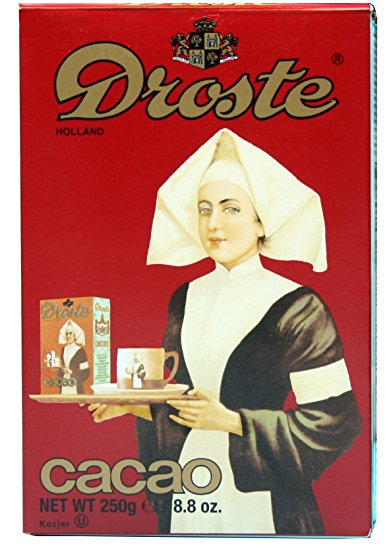
\includegraphics[height=1in]{background/pix/droste.jpg}
  \end{center}


  由于这款产品的关系，让一幅图片包含其自身的做法，有时也被称为
  德罗斯特效应。\index{Droste effect}
  % Can't get url to break: See also \protect\url{https://www.smithsonianmag.com/science-nature/fresh-off-the-3d-printer-henry-segermans-mathematical-sculptures-2894574/?no-ist}\index{self-reference}

  除了说谎者悖论，还有许多其他悖论。
  其中之一是 Quine（蒯因）悖论，\index{Quine's paradox}
  即一个断言自身为假的句子。


\begin{center}
    “当置于自身的引文之前时会产生假话” \\
    \quad 当置于自身的引文之前时会产生假话。
  \end{center}


  如果这个句子是假的，那么它所说的将是真话。
  如果这个句子是真的，那么它所说的就会成立，从而它就不是真的。

探讨这些及许多其他话题的一本精彩的大众读物是 \autocite{Hofstadter}。}。
换句话说，$\TM_m$ 的名字就是它的行为。

既然我们能够有效地从索引~$m$ 得到这台机器的源码，那么在某种意义上，这台机器是“知道”自己的源码的。
一个\citetext{\definend{蒯因（quine）}}{%
  以哲学家 Willard Van Orman Quine（威拉德·范·奥曼·蒯因）命名。}
是一个能输出自身源码的程序。
接下来，我们将逐步剖析构造一个蒯因的具体细节。\footnote{%
  最简单的这种程序会从磁盘上找到自己的源文件并把它打印出来。
  那是在作弊。}\index{quine program}\index{self reproducing program}
我们将使用 C 语言，因为它是低级语言，所以细节不会被隐藏。

我们可能会想，把源码本身作为一个字符串包含在源码中。
下面是一次这样的尝试，\footnote{%
  反斜杠-\protect\codeinline{n} 表示换行符。}
我们可以称之为 \codeinline{try0.c}。
但这太天真了。
那个字符串本身又得包含另一个字符串，如此等等。
就像小人理论一样，这会导致无穷倒退。
相反，我们需要一个程序，能以某种方式包含用于计算其自身一部分的指令。
\begin{lstlisting}
main() {
  printf("main(){\n ... }");
}
\end{lstlisting}

一种更巧妙的方法利用了我们对不动点定理的讨论，因为它在使用代码之前先提及代码。
这就是 \codeinline{try1.c}。\footnote{%
  \protect\codeinline{char *e="..."} 这个结构定义了一个字符串。
  在 C 语言的 \protect\codeinline{printf(...)} 命令中，第一个参数是一个字符串。
  在该字符串中，双引号会展开为单引号，
  \protect\codeinline{\%c} 会从随后的参数中取一个字符进行替换，
  而 \protect\codeinline{\%s} 会取一个字符串进行替换。}
\begin{lstlisting}
char *e="main(){printf(e);}"
main(){printf(e);};
\end{lstlisting}
以下是它的输出。
\begin{lstlisting}
main(){printf(e);};
\end{lstlisting}

将这一方法进一步升级，就得到了 \codeinline{try2.c}。
\begin{lstlisting}
char *e="main(){printf("char*e="");printf(e); printf("";\n");printf(e);"
main(){printf("char *e="");printf(e); printf("";\n");printf(e);}
\end{lstlisting}
这已经很接近了。
通过对一些换行符和引号进行转义\footnote{%
  数字 $10$ 是换行符的 ASCII 编码，34 是双引号的 ASCII 编码。}，
我们得到了这个能正常工作的程序 \codeinline{try3.c}。
\begin{lstlisting}
char *e="char*e="%c %s %c; %c main() {printf(e,34,e,34,10,10);}%c";
main(){printf(e,34,e,34,10,10);}
\end{lstlisting}

% A quine is a fixed point of an execution environment,
% when the execution environment is viewed as a function.
% Quines are possible in any complete model of
% computation; the exercises ask for them in a few languages.

% \subsection*{Know thyself}
% A program that prints itself can seem to be a parlor trick.
% But
% \citetext{for routines to have access to their code}{%
%   \definend{Introspection} is the ability to inspect code in the system,
%   such as to inspect the type of objects.
%   \definend{Reflection} is the ability to make modifications at runtime.}
% is useful.
% For example, to write a method \codeinline{toString(obj)}, you probably
% want your method to ask \codeinline{obj} for its source.
% Another example, more nefarious,
% is a computer virus that transmits copies
% of its code to other machines.

% \citetext{We will show how a routine can know its source}{%
%   This is derived from the wonderful presentation
%   in \autocite{Sipser}.}.
% We will start with an alternate
% presentation of a machine that prints itself.

% First, two technical points.
% One is that given two programs we can combine them into one, so that
% we run the first and then run the second.
% (Similarly,
% we can combine  two Turing  machines by
% renumbering the states so they do not conflict
% and then changing the final states in the first machine
% to have the number of the start state in the second.)

% The other point is
% that we have fixed a numbering of Turing machines that is
% `acceptable', meaning that there is a computable function from indices
% to machines and another computable function back.
% Write $\mathcal{T}$ for the set of Turing machines and
% let the function $\map{\strng}{\mathcal{T}}{\kleenestar{\B}}$
% input a Turing machine and return
% a standard bitstring representation of that machine (i.e., its source),
% let $\map{\mach}{\N}{\mathcal{T}}$
% input an index~$e$ and return the machine~$\TM_e$,
% and let $\map{\idx}{\kleenestar{\B}}{\N}$
% input the string representation of~$\TM_e$
% and return the index of that machine,~$e$
% (if the input string doesn't represent a Turing machine
% then it doesn't matter what this function does).
% Do this in such a way
% that $\idx$ is the inverse of the function $\composed{\strng}{\mach}$.

% Consider the machines sketched below.
% The first computes the
% function $\operatorname{echo}(\sigma,y)=\sigma$.
% Let it have index~$e_0$ and apply the \smn~theorem to get the
% family of machines sketched in the middle,  $\TM_{s(e_0,\sigma)}$,
% each of which ignores its input and just prints~$\sigma$.
% \begin{equation*}
%   \vcenteredhbox{\includegraphics{\asydir flowcharts/flowcharts13.pdf}}
%   \qquad
%   \vcenteredhbox{\includegraphics{\asydir flowcharts/flowcharts14.pdf}}
%   \qquad
%   \vcenteredhbox{\includegraphics{\asydir flowcharts/flowcharts15.pdf}}
% \end{equation*}
% On the right,
% $s(e_0,\sigma)$ is the index of the middle machine so
% $\composed{\strng}{\mach}(s(e_0,\sigma))$ is the standard string representation
% of the middle machine for~$\sigma$.
% Thus, if~$\sigma$ is the standard representation of a Turing machine~$\TM$ then
% when the machine on the right is done, the tape will contain only the standard
% representation of the middle machine for~$\sigma$, the machine that ignores
% its input and prints out~$\sigma$.
% Call the machine on the right~$\TM[Q]$ and call the function that it computes
% $\map{q}{\kleenestar{\Sigma}}{\kleenestar{\Sigma}}$.

% The machine that prints itself is a combination of two machines,
% $\TM[A]$ and~$\TM[B]$.
% Here's~$\TM[B]$.
% \begin{center}
%   \vcenteredhbox{\includegraphics{\asydir flowcharts/flowcharts16.pdf}}
% \end{center}
% The other machine is $\TM[A]=\TM_{s(e_0,\strng(\TM[B]))}$,
% which ignores anything on the tape and prints out
% the string representation of~$\TM[B]$.

% The action of the combination on an empty tape is that
% first the $\TM[A]$ part prints out the standard string representation
% $\strng(\TM[B])$.
% Then $\TM[B]$ reads it in as~$\beta$, computes
% $\alpha=\strng(\TM[A])$, concatenates the two string
% representations $\alpha\concat\beta$, and prints it.
% This is the string representation of itself, of the combination of
% $\TM[A]$ with~$\TM[B]$.

% To get a machine that computes with its own source
% we will extend this approach.
% The idea is to start with a machine~$\TM[C]$ that takes two inputs,
% a string representation of a machine and a string, and then
% get the desired machine~$\TM[D]$ that uses its own representation.

% \begin{theorem}
% For any Turing machine $\TM[C]$ that computes a two-input function
% $\map{c}{\kleenestar{\Sigma}\times\kleenestar{\Sigma}}{\kleenestar{\Sigma}}$
% there is a machine~$\TM[D]$ that computes a one-input function
% $\map{d}{\kleenestar{\Sigma}}{\kleenestar{\Sigma}}$
% where $d(\omega)=c(\strng(\TM[D]),\omega)$.
% \end{theorem}

% The machine~$\TM[D]$ is the combination of three machines, $\TM[A]$, $\TM[B]$,
% and~$\TM[C]$.
% First, as shown on the left,
% modify $\TM[Q]$ to write its output after a string already
% on the tape, because we need to leave the input~$\omega$ on the tape.
% \begin{center}
%   \vcenteredhbox{\includegraphics{\asydir flowcharts/flowcharts19.pdf}}
%   \qquad
%   \vcenteredhbox{\includegraphics{\asydir flowcharts/flowcharts20.pdf}}
% \end{center}
% Second, modify~$\TM[A]$ to be
% $\TM_{s(e_0,\strng(\TM[B])\concat\strng(\TM[C]))}$,
% which ignores anything on the tape and prints out
% the string representation
% of the combination of machines $\TM[B]$ and~$\TM[C]$.

% Next,
% as shown on the right, modify~$\TM[B]$ to
% input two strings, $\omega$ and~$\tau$.
% Apply~$q$ to the second to compute $\TM[A]$'s
% standard representation~$\alpha$.
% Print out the concatenation of $\alpha$ and~$\tau$, then a blank,
% and then the input~$\omega$.
% That has the form of two inputs;~finish by running the machine~$\TM[C]$ on
% them.

% \subsection*{Quining}
\citetext{动词 ‘to quine’}{%
  由 D~Hofstadter 发明。\index{Hofstadter, D}
  它可以追溯到哲学家 W~Quine 提出的陈述：
  \textit{“当置于自身引文之前时产生假话”当置于自身引文之前时产生假话}
  这句话具有悖论性质：如果它为真，则断言自身为假；如果为假，则必然为真。
  而且，它在没有直接自指的情况下做到了这一点。}
意思是：先写下一个句子片段，然后再写一遍，但这次要给它加上引号。
例如，从 `say` 我们得到 “say ‘say’.”。
另一个例子是 “quine ‘quine’.”。
这是自复制程序的语言学类比，其中第二个词扮演了传统程序/数据分离中数据的角色，
% http://www.madore.org/~david/computers/quine.html
这个角色与 \protect\codeinline{try3.c} 的第一行字符串所扮演的角色相同。
  %  ="char*e="%c %s %c; %c main() {printf(e,34,e,34,10,10);}%c";}
在“制造这台机器，然后执行这台机器”中，“制造”一词扮演的也是这个角色。

\citetext{我们可以用代码来表达这一点}{%
  本小节这一部分的内容源自
  \autocite{boro}\Dash
  “Boro”这个名字也来源于此\Dash 以及 \autocite{Avigad}。}。
首先考虑“引用”。
为了执行某个操作，我们通常定义一个函数，然后像 \codeinline{(f 1 2)} 这样调用它。
因此，如果我们想生成一个包含三个字符串的列表，那么下面的代码
\begin{lstlisting}
> (Boro is reading)
\end{lstlisting}
会产生错误：\codeinline{Boro:}\codeinline{undefined}。
我们必须告诉 Racket 不要对这些内容求值，在这个例子中，就是不要按通常方式对列表求值（将第一个条目当作函数，然后将其应用于其他条目的求值结果）。
\begin{lstlisting}
> (quote (Boro is reading))
'(Boro is reading)
\end{lstlisting}
有一个方便的单字符快捷方式。
\begin{lstlisting}
> '(Boro is reading)
'(Boro is reading)
\end{lstlisting}
我们可以把它做成一个函数。
\lstinputlisting[firstline=12,lastline=13]{scheme/background/quine-boro.rkt}
\begin{lstlisting}
> (P 'reading)
'(Boro is reading)
\end{lstlisting}
使用它就能得到\definend{对角化}例程。\index{diagonalization!routine}
\lstinputlisting[firstline=15,lastline=16]{scheme/background/quine-boro.rkt}
\begin{lstlisting}
> (Diag P 'reading)
'(Boro is '(Boro is reading))
\end{lstlisting}
这里是一个蒯因。
\lstinputlisting[firstline=24,lastline=25]{scheme/background/quine-boro.rkt}
\begin{lstlisting}
> (Quine-1 'reading)
'(reading 'reading)
> (Quine-1 'Quine-1)
'(Quine-1 'Quine-1)
\end{lstlisting}
% For a version that does not depend on the definitions use this.
% \begin{lstlisting}
% > ((lambda (x) (list x (list 'quote x)))
%  '(lambda (x) (list x (list 'quote x))))
% '((lambda (x) (list x (list 'quote x))) '(lambda (x) (list x (list 'quote x))))
% \end{lstlisting}
% The \codeinline{(lambda (x) ...)} construct is how Racket
% defines a function of one input without giving it a name
% (the term `lambda' comes from Church's Lambda Calculus).

\margingraphic{0.18\textwidth}{background/pix/thompson.jpg}{%
  \label{fig:thompson}\href{https://en.wikipedia.org/wiki/Ken_Thompson}{Ken Thompson（肯·汤普森） b~1943}}\index{Thompson, K!picture} % http://images.computerhistory.org/fellows/1997_ken_thompson.jpg
\subsection*{对信任的反思}\index{Reflections on Trusting Trust@\textit{Reflections on Trusting Trust}}
K~Thompson 是 UNIX 操作系统的两位主要创造者之一。
他职业生涯的大部分时间都在贝尔实验室工作，并且是 C 语言开发的核心人物。
他是正则表达式使用的先驱，并草拟了 Unicode 的 UTF-8 编码的定义。
近年来，他也是谷歌 Go 语言的创建者之一。

他曾获得计算机科学最高荣誉——图灵奖。
他在获奖演讲的开头是这样说的。

\begin{quotation}
上大学那会儿，还没有电子游戏，我们常常靠出编程题来互相消遣。
其中最受欢迎的题目之一，就是编写最短的自复制程序。
既然这是一项脱离现实的练习，
通常的工具就是 FORTRAN。
事实上，选择 FORTRAN 作为语言的理由，
和三人两足赛跑流行的理由是一样的。
\ldots{}\sentencespace
\end{quotation}

\vspace{-1.65ex} % picked by eye


\begin{quotation} % adding the extra quotation env makes K Thompson's outdent better
更精确地说，这个问题要求你编写一段源程序，
当其被编译并执行后，将产生一份与其源代码完全相同的副本作为输出。
% If you have never done this, I urge you to try it on your own.
% The discovery of how to do it is a revelation that far surpasses any
% benefit obtained by being told how to do it.
% The part about ``shortest'' was just an incentive to demonstrate skill
% and determine a winner.
\end{quotation}

这篇著名的文章构造了一个蒯因，
并展示了此类代码的存在如何构成一种极其微妙且几乎无法检测的安全威胁。
Thompson 的整个演讲 \autocite{Thompson} 流传很广；每个人都应该读一读。

% ...........................................
% \begin{exercises}
% \begin{exercise}
% Produce a Racket quine.
% \begin{credit}
%   \url{https://research.swtch.com/zip}
%   and
%   \href{http://cs.brown.edu/courses/gs019/asgn/hw3.sol.pdf}{Kevin Matulef}
% \end{credit}
% \begin{answer}
% % Here is a classic.
% % \begin{lstlisting}
% % ((lambda (x) `(,x ',x))
% % '(lambda (x) `(,x ',x)))
% % \end{lstlisting}
% %
% % This is due to Kevin Matulef.  % http://cs.brown.edu/courses/gs019/asgn/hw3.sol.pdf
% \lstinputlisting[firstline=3]{scheme/background/quine.rkt}
% \end{answer}
% \end{exercise}

% \begin{exercise}
% Produce a Python quine.
% \begin{credit}
%   \url{http://en.wikipedia.org/wiki/Quine_%28computing%29}
% \end{credit}
% \begin{answer}
% The python3 code
% \begin{lstlisting}
% # quine.py
% s = r"print('s = r\"' + s + '\"' + '\nexec(s)')"
% exec(s)
% \end{lstlisting}
% gives this command line output.
% \begin{lstlisting}
% $ python3 quine.py
% s = r"print('s = r\"' + s + '\"' + '\nexec(s)')"
% exec(s)
% \end{lstlisting} %$
% \end{answer}
% \end{exercise}

% % \begin{exercise}  %  p 75
% % \begin{credit}
% %   J~Avigad Computability and Incompleteness Lecture notes, % p 75
% %   \url{https://www.andrew.cmu.edu/user/avigad/Teaching/candi_notes.pdf}
% % \end{credit}
% % Consider a Scheme function \codeinline{diag} that is given a
% % string~$\sigma$ and returns a string with each instance of \str{x} in
% % $\sigma$ replaced with a quoted version of $\sigma$.
% % Thus \codeinline{diag("hello x world")} returns
% % \str{hello 'hello x world' world}.
% % Show that \codeinline{print(diag('print(diag(x))'))} is a quine.
% % \begin{answer}
% % \begin{lstlisting}
% % (define (diag s)
% %       (regexp-replace #rx"x" s s))
% % \end{lstlisting}
% % \end{answer}
% % \end{exercise}

% % \begin{exercise}
% % Write a program that defines a function
% % $f$ taking a string as input, and produces its output by applying
% % $f$ to its source code. For example, if $f$
% % reverses the given string, then the program should outputs its source code
% % backwards.
% % \end{exercise}

% % \begin{exercise}
% % Write a two-level polyglot quine, a program in one language
% % that outputs a program in a second language, which outputs the original program.
% % \end{exercise}
% \end{exercises}
\index{self reproduction|)}

% =======================================================
% \extra{Computer viruses}

% =======================================================
% \extra{A Universal Turing machine}

% =======================================================
\extra{忙海狸}\index{Busy Beaver|(}
% % \urldef{\radourl}{\url{https://math.osu.edu/about-us/history/tibor-rad%C3%B3}}
% \margingraphic{0.18\textwidth}{background/pix/rado1.png}{\label{fig:rado}\href{https://en.wikipedia.org/wiki/Tibor_Rad\%C3\%B3}{Tibor Rad\'o 1895--1965}}\index{Rado, T@Rad\'o, T!picture} % https://math.osu.edu/about-us/history/tibor-rad%C3%B3
对于任意~$n\in\N$，状态数不超过 $n$~的 Turing 机构成的集合是有限的。
因此，该集合中在空白纸带上会停机的 Turing 机 $\TM_e$ 只有有限多台。
我们可以思考，通过理解这些小型机器的行为，
我们能否获得关于计算（尤其是 Turing 机）的一般性洞见——例如，大多数 $n$ 状态 Turing 机会停机，还是只有少数会停机？

定义函数
$\map{\definend{\BB}}{\N}{\N}$ % \index{BB@$\BB$ (Busy Beaver) function}
给出最小步数，使得所有状态数为~$n$ 且在空白纸带上最终会停机的机器，到该步数时均已停机。
同时令
$\map{\definend{\Sigma}}{\N}{\N}$ % \index{Sigma@$\Sigma$ function}
为 $n$ 状态 Turing 机（从空白纸带启动）停机后留在纸带上的 \str{1} 数量的最大值。

\begin{theorem}[Rad\'o, 1962]
函数 $\BB$ 和 $\Sigma$ 是不可计算的。
\end{theorem}

\begin{proof}
如果~$\BB$ 是可计算函数，那么要判断某台 $\TM_e$ 在输入~$e$ 上是否停机，
我们只需让它运行 $\BB(n)$ 步。
如果 $\TM_{e}(e)$ 届时仍未停机，它就永远不会停机。
因此，$\BB$ 的可计算性将与停机问题（\HP）的不可解性相矛盾。
函数 $\Sigma$ 的情况类似，其证明留作练习 \zcref{exer:SigmaNotComputable}。
\end{proof}

这个 $\BB$ 看起来可能只是众多不可计算函数中的又一个而已。
然而，它有一个有趣的性质：任何增长速度比它快的函数 $f$——
即对所有足够大的~$n$ 满足 $f(n)\geq \BB(n)$——
同样也是不可计算的，其论证方法与前面证明中的相同。
于是，我们对什么使得一个函数不可计算获得了一种洞见：一种方式是增长得比任何可计算函数都快。\footnote{%
  注意这与 Ackermann 函数的联系，我们曾指出 Ackermann 函数不是原始递归的，
  因为它增长得比任何原始递归函数都快。}

% \margingraphic{0.25\textwidth}{background/pix/beaver.jpg}{\label{fig:beaver}\href{http://commons.wikimedia.org/wiki/File:Beaver_\%28PSF\%29.jpg}{Rare moment of rest}}
% \urldef{\radourl}{\url{https://math.osu.edu/about-us/history/tibor-rad%C3%B3}}
\margingraphic{0.18\textwidth}{background/pix/rado1.png}{\label{fig:rado}\href{https://en.wikipedia.org/wiki/Tibor_Rad\%C3\%B3}{Tibor Rad\'o 1895--1965}}\index{Rado, T@Rad\'o, T!picture} % https://math.osu.edu/about-us/history/tibor-rad%C3%B3
\definend{忙海狸问题}\index{Busy Beaver problem@\probname{Busy Beaver} problem}
是：\citetext{哪台 $n$ 状态 Turing 机在停机前能做最多的计算工作}{%
  R~H Bruck 曾写道 \autocite{Bruck}：
  “我可以把高速计算机比作一支巨大而笨拙的铅笔，
  它需要很长时间才能削好，也无法用通常的方式用手指握持，
  给人以能响应我心意的错觉；
  但它却配备了一台相当精密的引擎，
  只要我愿意让它在很大程度上支配书写的主题，
  它就会像疯了一样疯狂书写。”
  忙海狸机就是该规模下最疯狂的书写者。
}？

\citetext{可以把这看作一场竞赛}{%
  关于这个主题有两个非常精彩的视频：
  YouTube 频道 Mutual Information 的
  \href{https://www.youtube.com/watch?v=kmAc1nDizu0}{\textit{计算的边界}}
  和
  \href{https://www.youtube.com/watch?v=jlh21U2texo}{\textit{在计算的边界会发生什么？}}。}
看谁能构造出达到极限值~$\BB(n)$ 或~$\Sigma(n)$ 的机器。\footnote{%
  在这个问题由 T~Rad\'o 首次提出后的许多年里，
  竞赛主要围绕 $\Sigma$ 展开。
  不过，最近大家更常讨论 $\BB$。
  无论如何，这两者关系非常密切。}
计算需要规则，此处的传统是固定一种 Turing 机的定义：它具有一端无限延伸的纸带，
使用两个纸带符号 \str{1} 和~\str{B}，
有一个不计入机器状态总数的独立停机状态，
机器从空白纸带开始运行，
且转移的形式为
$\Delta(\text{state}, \text{tape symbol})
  =\sequence{\text{state}, \text{tape symbol}, \text{head shift}}$。

\subsection*{已知结果}
\citetext{在 1962 年的论文中，Rad\'o}{%
  这篇论文 \autocite{Rado} 异常清晰且有趣。}
解决了 $n=0$、$n=1$ 和 $n=2$ 的情况
（$n=0$ 是平凡的，因为此时机器仅由停机状态组成）。
1964 年，Rad\'o 和 Lin 证明了 $\Sigma(3)=6$。


\begin{example}
这是三状态的忙海狸机器，停机状态是~$q_3$。
\begin{center}  \small
\begin{transitionfunction}
        &\str{B}  &\str{1}  \\ \cline{2-3}
  $q_0$ &$q_1,\str{1},R$  &$q_3,\str{1},R$        \\
  $q_1$ &$q_2,\str{B},R$  &$q_1,\str{1},R$        \\
  $q_2$ &$q_2,\str{1},L$  &$q_0,\str{1},L$
\end{transitionfunction}
\end{center}
\end{example}


1983 年，A~Brady 证明了 $\Sigma(4)=13$ 和 $\BB(4)=107$。

\citetext{2024 年，一组研究人员}{%
  参见 \autocite{Brubaker}} 通过互联网协作，并使用 Coq 证明验证系统，证明了
$\Sigma(5)=4\,098$ 以及 $\BB(5)=47\,176\,870$。
他们的机器计算 $g(0)$, $g(g(0))$, \ldots{} 直到停机，其中
$g$ 是这个函数。
\begin{equation*}
  g(n)=
  \begin{cases}
    (5n+18)/3  &\case{if $n$ leaves a remainder of $0$ on division by $3$}  \\
    (5n+22)/3  &\case{if $n$ leaves a remainder of $1$}  \\
    \text{停机}&\case{otherwise}
 \end{cases}
\end{equation*}

下表总结了
\citetext{当前记录}{%
  最新的是 BB(6) 的结果，由 BBchallenge 团队成员 mxdys 于 2025 年 6 月得出。}。

\begin{center}\small
  \begin{tabular}{r|cccccc}
    $n$         &$1$  &$2$  &$3$  &$4$   &$5$           &$6$ \\ \cline{2-7}
    \begin{tabular}[t]{@{}r@{}}
      $\BB(n)$  \\
      $\Sigma(n)$
    \end{tabular}
    &\begin{tabular}[t]{@{}r@{}}
      $1$ \\
      $1$
    \end{tabular}
    &\begin{tabular}[t]{@{}r@{}}
      $6$ \\
      $4$
    \end{tabular}
    &\begin{tabular}[t]{@{}r@{}}
      $21$ \\
      $6$
    \end{tabular}
    &\begin{tabular}[t]{@{}r@{}}
      $107$ \\
      $13$
    \end{tabular}
    &\begin{tabular}[t]{@{}r@{}}
      $47\,176\,870$  \\
      $4\,098$
    \end{tabular}
    &\rule{0em}{2.25ex}\begin{tabular}[t]{@{}l@{}}
      $\geq \prescript{9}{}{\prescript{2}{}{\prescript{2}{}{2}}}$
      \rule{0pt}{13pt}
      \\
      $\geq \prescript{15}{}{10}$ %\uparrow\uparrow 15
    \end{tabular}
  \end{tabular}
\end{center}

左上标记法表示四级超运算，即迭代幂运算。
因此，$\prescript{9}{}{2}$ 表示 $2$ 的 $2$ 次幂的 $2$ 次幂 \ldots{}，共迭代九次。

\subsection*{如何寻找这些值}
在 $n=2$ 之后，解决这个问题的显然方法是使用广度优先搜索：$n$~状态的机器只有有限多台，因此
让它们全部在空白纸带上运行，进行交错并行，
然后静观其变。
这能快速判定大量机器的情况。
当然，其中一些机器不会停机，或者运行时间超出我们的耐心。
对于其中部分机器，从其源代码很容易判断其行为，我们有望将范围快速缩小到相对较少的机器进行深入研究，
从而通过穷举法找到该~$n$ 的答案。\footnote{%
  \protect\citetext{Brady}{参见 \protect\autocite{Brady}} 报告称，对于 $n=4$，
  这样的机器有 $5\,280$ 台。}

但是，如果对于某个~$n$，我们找到一台计算着某些我们未知之物的机器呢？
例如，如果 $n$ 足够大，以至于能容许一台机器当且仅当找到
\citetext{奇完全数}{%
  如果一个数等于其所有真因子之和，则称为完全数。
  例如，$6=1+2+3$。
  偶完全数是存在的，但我们不知道奇完全数是否存在。}
时才停机呢？
$n=6$ 的情况似乎就存在一台类似的机器。

如需了解更多信息，有许多网站涵盖了这一主题，包括最新的结果。
除了维基百科页面外，最经典的网站是 \href{https://bbchallenge.org}{\texttt{bbchallenge.org}}。
有些网站讨论了机器标准的变体，例如考虑
\citetext{具有三个或更多符号的机器}{%
  具有三个状态和三个符号的机器的情况仍然未知。
  求解它需要解决一个类似 Collatz 的问题，目前无人能做到。
  参见
  \url{https://www.sligocki.com/2023/10/16/bb-3-3-is-hard.html}。}。

忙海狸数不仅极难寻找，而且在某一点之后会变得根本无法求解。
2016 年，A~Yedida 和 S~Aaronson 得到了一个 $n$，使得
\citetext{$\BB(n)$ 不可知}{%
  参见 \autocite{Aaronson16} 以及优秀的综述 \autocite{Aaronson20}
  和 \autocite{Aaronson25}。
  另见 \url{https://www.quantamagazine.org/the-busy-beaver-game-illuminates-the-fundamental-limits-of-math-20201210/}。}。
为此，他们创建了一种编程语言，其程序可编译成 Turing 机。
利用该语言，他们构造了一台
\citetext{7918 状态的 Turing 机}{%
  所需的状态数此后已被减少。
  截至本书写作时，它已降至 $748$ 个状态。
  参见 J~Riebel 优秀的学士学位论文：
  \url{https://www.ingo-blechschmidt.eu/assets/bachelor-thesis-undecidability-bb748.pdf}。}，
如果\citetext{数学的标准公理}{%
  这是 ZFC，即带有选择公理的 Zermelo–Fraenkel 公理。
  （此外，他们还假定了静止 Ramsey 性质假设。）}中存在矛盾，则该机停机；
如果这些公理是一致的，则永不停机。
我们相信这些公理是一致的，因此我们相信这台机器不会停机。
然而，Gödel 第二不完备定理表明，无法用公理本身来证明这些公理是一致的。
因此，在这种情况下，\probname{Busy Beaver} 问题的解是不可知的，因为即使我们得到了数 $\BB(n)$，也无法用我们的公理证明它是正确的，即证明这台机器会停机。
% (They also produced an explicit
% Turing machine that halts if and only if there is a counterexample to Goldbach’s
% conjecture, and one that halts if and only if the Riemann hypothesis
% is false.)

总而言之，函数不可计算的一种方式是其增长速度快于任何可计算函数。
但要注意，这并不是唯一的方式。
存在一些函数，它们的增长速度慢于某些可计算函数，却仍然是不可计算的。

\begin{exercises}
% \recommended
% \begin{exercise}
% Give the computation history, the sequence of configurations, that come from
% running the three-state Busy Beaver machine.
% \hint~you can run it on the Turing machine simulator.
% \end{exercise}


\begin{exercise}
讨论中用到的这种风格的 Turing 机共有多少台？
\begin{answer}\verified
函数 $\Delta$ 有 $n\cdot 2$ 个输入和 $(n+1)\cdot  2\cdot 2$ 个输出。
因此共有 $(2n)^{4(n+1)}$ 台机器。
\end{answer}
\end{exercise}

\recommended


\begin{exercise}
编写并运行一个例程来计算 $g(0)$、$g(g(0))$，……。
\begin{answer}\verified
\figureref{fig:RacketBB5} 中的 Racket 代码可以计算它。
\begin{figure}
  \centering
  \lstinputlisting[firstline=3]{background/scheme/BB5.rkt}
  \caption{产生计算 $\BB (5)$ 过程中所发现值的 Racket 代码。}
  \label{fig:RacketBB5}
\end{figure}
值依次为 $6$、
$16$、
$34$、
$64$、
$114$、
$196$、
$334$、
$564$、
$946$、
$1584$、
$2646$、
$4416$，
$7366$、
以及 $12284$。
\end{answer}
\end{exercise}

% \recommended
% \begin{exercise}
% \begin{exparts*}
% \item
% How many Turing machines with tape alphabet $\set{\str{B},\str{1}}$
% are there having one state?
% \item
% Two?
% \item
% How many with $n$~states?
% \end{exparts*}
% \end{exercise}

% \begin{exercise}
% How many Turing machines are there, with a tape alphabet
% $\Sigma$ of $n$ characters and having $n$~states?
% \begin{answer}
% $\bigl( 2(c+1)(n+2) \bigr)^{(c+1)n}$
% \end{answer}
% \end{exercise}

% \begin{exercise}
% Give $\TM[M]_1$ and $\TM[M]_2$, the Turing machines
% having $1$ and~$2$ states that write $1$ and $2$-many \str{1}'s to a blank tape.
% \end{exercise}

\recommended


\begin{exercise}
给出一个最终将超过任何可计算函数的函数的对角化构造。
\begin{answer}\verified
本题并未要求我们构造一个可计算函数；事实上，这样的可计算函数根本不存在。

如果 $\TMfcn_0(0)$ 收敛，则定义 $f(0)$ 为 $1+\TMfcn_0(0)$；否则定义 $f(0)=1$。
（注意 $f$ 不是可计算函数。）
类似地，定义 $f(1)$ 为 $1+f(0)$、$1+\TMfcn_0(1)$ 与 $1+\TMfcn_1(1)$ 三者的最大值，
若后两项中任意一项发散，则不将其计入最大值中。
对所有 $n$ 同理定义。

更形式化地，若 $\TMfcn_e(x)$ 收敛，则定义 $F(e,x)$ 为 $\TMfcn_e(x)$，否则为 $0$。
那么 $f(i)$ 就是 $\set{F(0,i),\ldots F(i,i)}$ 的最大值再加 $1$。
\end{answer}
\end{exercise}

\recommended

\begin{exercise}
证明存在不可计算函数，其增长速度不快于可计算函数 $f(x)=1$。
\hint~用可数性论证。
\begin{answer}
根据提示，注意到输出在集合 $\set{0,1}$ 中的函数有不可数多个，
即每个输出都小于或等于 $1$。
Turing 机只有可数多个，所以可计算函数只有可数多个，
因此输出以 $1$ 为界的可计算函数也只有可数多个。
故存在输出以 $1$ 为界的不可计算函数。
\end{answer}
\end{exercise}

\begin{exercise} \label{exer:SigmaNotComputable}
这是关于 $\Sigma$ 不可计算的证明。
设 $\map{f}{\N}{\N}$ 是任意全可计算函数。
我们将证明对无穷多个 $n$ 有 $\Sigma(n)>f(n)$，因此 $\Sigma\neq f$。
\begin{exparts}
\item
证明存在一台具有 $j$ 个状态的 Turing 机 $\TM[M]_j$，
它能在空白纸带上写下 $j$ 个 \str{1}。
\item
令 $\map{F}{\N}{\N}$ 为这个函数。
\begin{equation*}
  F(m) % = \sum_{0\leq i< m+1} f(i)+i^2  % using \Sigma so omit summation
       = (f(0)+0^2)+(f(1)+1^2)+(f(2)+2^2)+\cdots+(f(m)+m^2)
\end{equation*}
论证它具有以下三个性质：若 $0<m$，则 $f(m)<F(m)$，
且 $m^2\leq F(m)$，
以及 $F(m)<F(m+1)$。
\item
下面的插图展示了两台 Turing 机的组合。
在右侧，我们将左侧第一台机器的接受状态与第二台机器的初始状态合并。
\begin{center}
  \vcenteredhbox{\includegraphics{\asydir busybeaver/busybeaver01.pdf}}
  \hspace{2.5em}
  \vcenteredhbox{\includegraphics{\asydir busybeaver/busybeaver02.pdf}}
\end{center}
考虑 Turing 机 $\TM$，它先执行 $\TM[M]_j$，
然后执行 $\TM[M]_F$，接着再执行一次 $\TM[M]_F$。
证明它的生产力为 $F(F(j))$，且具有 $j+2n_F$ 个状态。

\item
最后，与具有 $j+2n_F$ 个状态的忙海狸机比较。
根据定义，
$F(F(j))\leq \Sigma(j+2n_F)$。
因为 $n_F$ 是机器 $\TM[M]_F$ 的状态数，为常数，所以关系 $j+2n_F\leq j^2< F(j)$
对足够大的 $j$ 成立。
请论证
$f(j+2n_F) \leq \Sigma(j+2n_F)$。
\end{exparts}
\begin{answer}\verified
\begin{exparts}
\item
最好用一个例子来回答：这里是 $\TM[M]_4$。
\begin{center}
  \includegraphics{\asydir busybeaver/busybeaver00.pdf}
\end{center}
\item
第一个性质成立是因为 $f(m)$ 是 $F(m)$ 表达式中的一个求和项；
类似地，第二个性质成立是因为 $m^2$ 也是一个求和项。
第三个性质成立是因为当 $m>0$ 时所有求和项均为正数。

\item
如果从空白纸带开始，这台机器首先产生 $j$ 个 \str{1}，
然后产生 $F(j)$ 个 \str{1}，最终在纸带上留下 $F(F(j))$ 个 \str{1}。
因此其生产力为 $F(F(j))$。

\item
由于 $F$ 严格递增，$F(j+2n_F)<F(F(j))$。
结合得到
$
   f(j+2n_F) <
   F(j+2n_F) <
   F(F(j))
   \leq \Sigma(j+2n_F)$，
如所需。
\end{exparts}
\end{answer}
\end{exercise}

% Copy this back to the proof?
% For $\Sigma$,
% let $\map{f}{\N}{\N}$ be any total computable function.
% We will show that
% $\Sigma(n)>f(n)$ for infinitely many~$n$,
% and so $\Sigma\neq f$.
%
% First note that there is a Turing Machine $\TM[M]_j$
% having $j$~many states that writes $j$-many \str{1}'s to a blank tape.
% For instance, here is $\TM[M]_4$.
% \begin{center}
%   \includegraphics{\asydir busybeaver/busybeaver00.pdf}
% \end{center}
% Also note that we can compose two Turing machines.
% The illustration below shows two machines on the left.
% On the right, we have combined the final states
% of the first machine with the start state of the second.
% \begin{center}
%   \vcenteredhbox{\includegraphics{\asydir busybeaver/busybeaver01.pdf}}
%   \hspace{2.5em}
%   \vcenteredhbox{\includegraphics{\asydir busybeaver/busybeaver02.pdf}}
% \end{center}
%
% Let $\map{F}{\N}{\N}$ be this function.
% \begin{equation*}
%   F(m) % = \sum_{0\leq i< m+1} f(i)+i^2  % using \Sigma so omit summation
%        = (f(0)+0^2)+(f(1)+1^2)+(f(2)+2^2)+\cdots+(f(m)+m^2)
% \end{equation*}
% It has the properties:~if $0<m$ then $f(m)<F(m)$,
% and $m^2\leq F(m)$,
% and $F(m)<F(m+1)$.
% It is intuitively computable so Church's Thesis says there is a
% Turing machine $\TM[M]_F$ that computes it.
% Let that machine have $n_F$~many states.
%
% Now consider the Turing machine $\TM$
% that performs $\TM[M]_j$ and follows that with the machine
% $\TM[M]_F$, and then follows that with another copy of the machine
% $\TM[M]_F$.
% If started on a blank tape this machine will first produce $j$-many \str{1}'s,
% then produce $F(j)$-many \str{1}'s, and finally will leave the tape with
% $F(F(j))$-many \str{1}'s.
% Thus its productivity is
% $F(F(j))$.
% It has $j+2n_F$ many states.

% Compare that with the $j+2n_F$-state Busy Beaver machine.
% By definition
% $F(F(j))\leq \Sigma(j+2n_F)$.
% Because $n_F$ is constant (it is the number of states in
% the machine $\TM[M]_F$), the relation $j+2n_F\leq j^2< F(j)$
% holds for sufficiently large~$j$.
% Since $F$ is strictly increasing, $F(j+2n_F)<F(F(j))$.
% Combining gives
% $
%    f(j+2n_F) <
%    F(j+2n_F) <
%    F(F(j))
%    \leq \Sigma(j+2n_F)$,
% as required.

\end{exercises}
\index{Busy Beaver|)}

% =============================
% For defn of \cantorfile see src/directory.tex
\extra{用代码实现 Cantor 对应}  \label{sec:CantorInCode}
在本节中，我们以最直接的方式证明 $\N$ 和 $\N\times\N$ 之间的 Cantor 对应是能行的：我们给出代码。

回顾在下表中
\begin{equation*}
  \begin{array}{r|cccccc@{\hspace{6pt}}c}
    \tabulartext{$n\in\N$}
      &0 &1 &2 &3 &4 &5 &\ldots
      \\ \cline{2-8}
    \tabulartext{$\sequence{i,j}\in\N\times\N$}
      &\sequence{0,0} \rule{0em}{2ex} % make room above angle brackets
      &\sequence{0,1}
      &\sequence{1,0}
      &\sequence{0,2}
      &\sequence{1,1}
      &\sequence{2,0}
      &\ldots
  \end{array}
\end{equation*}
%</table:CrossProductCorrespondence>
%<*def:PairingFcn>
从顶行到底行的映射是 Cantor
配对函数\index{pairing function}\index{function!pairing}，
因为它输出数对；而从底行到顶行的逆映射是
解配对函数\index{unpairing function}\index{function!unpairing}。

首先是解配对。
给定 $\sequence{x,y}$，我们用 $1+2+\cdots n=n(n+1)/2$ 确定它所在的对角线，
\lstinputlisting[firstline=17,lastline=22]{\cantorfile}
然后利用它来找到值 $(1+2+\cdots x)+y$。
\lstinputlisting[firstline=33,lastline=38]{\cantorfile}

使用这个函数很容易。
\begin{lstlisting}
$ racket
Welcome to Racket v8.3 [cs].
> (require "counting.rkt")
> (cantor-unpairing 1 1)
4
> (cantor-unpairing 34 10)
1024
>
\end{lstlisting} % $

我们可能会想，\codeinline{cantor-unpairing} 的参数
应该是如上所得的两个数 $x$ 和 $y$，
还是数对 $\sequence{x,y}$。
但这并不太重要，因为如果我们需要这个数对，
可以改用 \codeinline{apply} 操作符。
\begin{lstlisting}
> (cantor-unpairing 10 12)
263
> (apply cantor-unpairing '(10 12))
263
\end{lstlisting} % $

接下来，介绍配对函数。
给定一个自然数 $c$，为了找到对应的数对 $\sequence{x,y}$，我们首先要找到它落在哪条对角线上。
对角线为 $d(x,y)=x+y$，设对应的三角数为$t(x,y)=d(d+1)/2=(d^2+d)/2$。
于是有 $0=d^2+d-2t$。
应用熟悉的公式$(-b\pm\sqrt{b^2-4ac})/(2a)$可得：
\begin{equation*}
  d=\frac{-1+\sqrt{1-4\cdot 1\cdot (-2t)}}{2\cdot 1}
   =\frac{-1+\sqrt{1+8t}}{2}
\end{equation*}
（我们只保留了 $\pm$ 中的 $+$ 号，因为另一个根是负数。）
给定配对函数的输入~$c$，为了找到包含满足 $\pair(x,y)=c$ 的数对 $\sequence{x,y}$ 的那条对角线的编号，
\citetext{使用取底函数}{%
  设第 $n$ 个三角数为
  $t(n)=0+1+\cdots+n=n(n+1)/2$。
  函数~$t$ 是单调递增的，并且存在无穷多个三角数。
  因此，对于每个自然数~$c$，都存在唯一的最大三角数 $t(n)$，使得 $c=t(n)+k$ 对某个~$k\in\N$ 成立。
  因为$t(n+1)=t(n)+n+1$，我们看到 $k<n+1$，即 $k\leq n$。
  所以，要从数对的 Cantor 编号~$c$ 计算对角线编号~$d$，我们有$(1/2)d(d+1)\leq c< (1/2)(d+1)(d+2)$。
  应用二次求根公式的左右两部分，得到$(1/2)(-3+\sqrt{1+8c})<d\leq (1/2)(-1+\sqrt{1+8c})$。
  令$(1/2)(-1+\sqrt{1+8c})$为 $\alpha$，则有$c\in\rightclosed{\alpha-1}{\alpha}$，因此 $d=\floor{\alpha}$。
  \autocite{222835}}，
$d=\floor{(-1+\sqrt{1+8c})/2}$。
% \footnote{
%   The code for \codeinline{diag-num} has and implementation detail of interest.
%   The code leads to numbers large enough to
%   give floating point overflows.
%   For instance, \protect\codeinline{(cantor-n 1 2 3 4 5 6 7)} returns
%   \protect\codeinline{1.05590697087673e+55}.
%   }

\lstinputlisting[firstline=58,lastline=63]{\cantorfile}
然后，通过查看~$c$ 沿这条对角线走了多远，我们就能得到 $\sequence{x,y}$。
\lstinputlisting[firstline=75,lastline=81]{\cantorfile}

\noindent 以自然的方式使用它。

\begin{lstlisting}
> (cantor-pairing 15)
'(0 5)
> (cantor-pairing (cantor-unpairing 10 12))
'(10 12)
\end{lstlisting}

有了这些，我们就可以重现本节开头的表格了。

\begin{lstlisting}
> (for ([i '(0 1 2 3 4 5)])
     (displayln (cantor-pairing i)))
(0 0)
(0 1)
(1 0)
(0 2)
(1 1)
(2 0)
\end{lstlisting}

扩展到三元组是直截了当的。
这些例程的命名或许不太恰当\Dash 它们可能更适合被命名为
\codeinline{cantor-tupling-3} 和 \codeinline{cantor-untupling-3}\Dash
但我们将沿用已有的名称。

\lstinputlisting[firstline=107,lastline=110]{\cantorfile}
\lstinputlisting[firstline=122,lastline=126]{\cantorfile}

\noindent
使用这些例程也很直接。

\begin{lstlisting}>
> (cantor-pairing-3 172)
'(1 2 3)
> (for ([i '(0 1 2 3 4 5 6 7 8 9)])
     (displayln (cantor-pairing-3 i)))
(0 0 0)
(0 0 1)
(1 0 0)
(0 1 0)
(1 0 1)
(2 0 0)
(0 0 2)
(1 1 0)
(2 0 1)
(3 0 0)
\end{lstlisting}

类似的例程也适用于四元组。

\lstinputlisting[firstline=147,lastline=150]{\cantorfile}
\lstinputlisting[firstline=162,lastline=167]{\cantorfile}

以下是前几个四元组。

\begin{lstlisting}
> (for ([i '(0 1 2 3 4 5 6)])
    (displayln (cantor-pairing-4 i)))
(0 0 0 0)
(0 0 0 1)
(1 0 0 0)
(0 1 0 0)
(1 0 0 1)
(2 0 0 0)
(0 0 1 0)
\end{lstlisting}

% From url.sty; need this because the url has a percent sign in it.
\urldef{\yagni}\url{https://en.wikipedia.org/wiki/You_aren%27t_gonna_need_it}
三元组和四元组的例程表明，存在一个通用的模式。
何妨一试，就当好玩，
\citetext{我们可以扩展到任意大小的元组}{%
  参见 \yagni。}。

对于函数$\map{\unpair}{\N^k}{\N}$（我们也称它为 $\cantor$），我们可以通过查看输入参数的个数来确定 $k$。
因此，\codeinline{cantor-unpairing-n} 通过接受任意长度的元组，推广了
\codeinline{cantor-unpairing}、\codeinline{cantor-unpairing-3} 等函数。

\lstinputlisting[firstline=195,lastline=203]{\cantorfile}

\begin{lstlisting}
> (cantor-unpairing-n 0 0 1 0)
6
> (cantor-unpairing-n 1 2 3 4)
159331
\end{lstlisting}

要推广到函数$\map{\pair}{\N}{\N^k}\!$，
棘手的地方在于，这个例程无法知道目标元数~$k$，我们必须单独指定它。

\lstinputlisting[firstline=226,lastline=239]{\cantorfile}

\noindent
这展示了该例程如何像 \codeinline{cantor-pairing-4} 一样工作。

\begin{lstlisting}
> (for ([i '(0 1 2 3 4 5 6)])
    (displayln (cantor-pairing-arity 4 i)))
(0 0 0 0)
(0 0 0 1)
(1 0 0 0)
(0 1 0 0)
(1 0 0 1)
(2 0 0 0)
(0 0 1 0)
\end{lstlisting}

例程 \codeinline{cantor-pairing-arity} 并非一致的，因为它一次只能处理一种元数。
换句话说，\codeinline{cantor-unpairing-arity} 并非 \codeinline{cantor-pairing-n} 的逆函数，因为我们必须告诉它元组的元数。

\begin{lstlisting}
> (cantor-unpairing-n 3 4 5)
1381
> (cantor-pairing-arity 3 1381)
'(3 4 5)
\end{lstlisting}

为了覆盖所有长度的元组，
为了在自然数与自然数序列集合之间建立对应，
我们定义两个匹配的例程：
\codeinline{cantor-pairing-omega} 和 \codeinline{cantor-unpairing-omega}。

\begin{lstlisting}
> (for ([i '(0 1 2 3 4 5 6 7 8)])
    (displayln (cantor-pairing-omega i)))
()
(0)
(0 0)
(1)
(0 1)
(0 0 0)
(2)
(1 0)
(0 0 1)
\end{lstlisting}

\codeinline{cantor-pairing-omega} 的思路是，
将其输入 \codeinline{c} 解释为一个数对 $\sequence{x,y}$，即 $c=\pair(x,y)$。
然后它返回一个长度为~$x+1$ 的元组，其中~$y$ 是这个元组的 Cantor 编号。
（长度为 $x+1$ 而非 $x$ 的原因是：
空元组与 $c=0$ 相关联。
接着，为了避免所有后续的数对 $\sequence{0,y}$ 不与任何数相关联，
我们接下来使用一元组 $\sequence{0}$，
之后使用 $\sequence{1}$，依此类推。）

\lstinputlisting[firstline=286,lastline=296]{\cantorfile}

\lstinputlisting[firstline=274,lastline=284]{\cantorfile}

这展示了它们的用法。

\begin{lstlisting}
> (cantor-unpairing-omega 1 2 3 4)
12693741448
> (cantor-pairing-omega 12693741448)
'(1 2 3 4)
\end{lstlisting}

\begin{exercises}


\begin{exercise}
Cantor 编号 $42$ 对应哪个数对？
\begin{answer}\verified
\begin{lstlisting}
> (cantor-pairing 42)
'(6 2)
\end{lstlisting}
\end{answer}
\end{exercise}

\begin{exercise}
Cantor 编号 $666$ 对应哪个数对？
\begin{answer}\verified
\begin{lstlisting}
> (cantor-pairing 666)
'(0 36)
\end{lstlisting}
\end{answer}
\end{exercise}

% \begin{exercise}
% What is the formula for the gaps between one-tuples?
% \begin{answer}\verified
% The first gap has size zero, the next has size one, etc.
% \end{answer}
% \end{exercise}

\begin{exercise}
第一个由 \codeinline{cantor-pairing-omega} 映射到四元组的数是哪个？
\begin{answer}\verified
\begin{lstlisting}
> (cantor-unpairing 3 0)
9
> (for ([i '(0 1 2 3 4 5 6 7 8 9)])
    (display (cantor-pairing-omega i)) (newline))
()
(0)
(0 0)
(1)
(0 1)
(0 0 0)
(2)
(1 0)
(0 0 1)
(0 0 0 0)
\end{lstlisting}
\end{answer}
\end{exercise}


\end{exercises}

% \subsection*{Numbering Turing machines}
% We will define a correspondence between natural
% numbers and Turing machines
% via Scheme code.

% We represent an instruction with
% four-tuple of natural numbers.
% In the code below this is a \codeinline{quad}.
% A Turing machine is then represented as
% a list, a \codeinline{quadlist}.

% To go from a number to a \codeinline{quadlist} we first apply
% \codeinline{xy-omega}.
% This
% turns the number into a sequence of numbers,
% below called a \codeinline{numlist}.
% We convert each of its numbers into a \codeinline{quad}
% to get a \codeinline{quadlist}.

% \lstinputlisting[firstline=134,lastline=150]{background/scheme/godelnumbering.scm}

% This illustrates.
% The last line associates the number $2558$ with the three-element
% \codeinline{quadlist}.
% \begin{lstlisting}
% #;1> (natural->quad 1)
% (0 0 0 1)
% #;2> (natural->quad 2)
% (1 0 0 0)
% #;3> (natural->quad 3)
% (0 1 0 0)
% #;4> (cantor-omega 3 2 1)
% 2558
% #;5> (get-nth-quadlist 2558)
% ((0 1 0 0) (1 0 0 0) (0 0 0 1))
% \end{lstlisting}

% A Turing machine is a set so to check if a \codeinline{quadlist}
% is a Turing machine we must
% check that no two quads are the same.
% In addition, a Turing machine is deterministic, so different
% \codeinline{quad}'s must begin with different first two numbers.
% The second condition implies the first, so only the second is checked here.

% \lstinputlisting[firstline=152,lastline=196]{background/scheme/godelnumbering.scm}

% We count Turing machines by brute force, convert each candidate to a
% \codeinline{quadlist}, and test whether it is a Turing machine.
% \lstinputlisting[firstline=209,lastline=212]{background/scheme/godelnumbering.scm}

% \lstinputlisting[firstline=209,lastline=212]{background/scheme/godelnumbering.scm}

% With that, here is the function that takes in a Turing machine as a list of
% quads and finds a natural number index for that Turing machine, along with
% the inverse function, taking the machine to an index for its machine.

% \lstinputlisting[firstline=216,lastline=230]{background/scheme/godelnumbering.scm}

% % Inverse to the prior routine, this inputs a natural number and returns
% % the Turing machine with that natural number index.

% % \lstinputlisting[firstline=225,lastline=230]{background/scheme/godelnumbering.scm}

% Use is straightforward.
% The last one takes a few seconds.

% \begin{lstlisting}
% #;2> (machine 0)
% ()
% #;3> (machine 1)
% ((0 0 0 0))
% #;4> (machine 2)
% ((0 0 0 1))
% #;5> (machine 3)
% ((1 0 0 0))
% #;6> (godel '((0 0 0 0)))
% 1
% #;7> (godel '((0 1 1 1)))
% 298
% \end{lstlisting}

% % This enumeration
% % is said to be \definend{acceptable} because it has three key properties:
% % (1)~there is a routine, here \codeinline{godel}, that takes us
% % from the source code of a Turing machine, from the list of instructions,
% % to an associated number;
% % (2)~there is a routine, here \codeinline{machine}, that goes
% % from a number to the associated source,
% % and
% % (3)~the set of numbers for which there is an associated machine is computable
% % (in the case of this enumeration, this set is all natural numbers although
% % other numberings exist; see \zcref{exer:OtherNumberings}).

% Earlier we saw a Turing machine simulator.
% We can translate the machines written here to the earlier format.
% That is, we can interpret each of the \codeinline{quad}'s above
% \codeinline{(a0 a1 a2 a3)}
% as an instruction $(q_p,T_p,T_n,q_n)$.

% \lstinputlisting[firstline=295,lastline=320]{background/scheme/godelnumbering.scm}

% These rely on helper routines.
% Handling the states is trivial: for instance, $\text{\codeinline{a0}}=0$
% and $\text{\codeinline{a3}}=0$
% translate to the state~$q_0$.

% \lstinputlisting[firstline=257,lastline=261]{background/scheme/godelnumbering.scm}

% \lstinputlisting[firstline=290,lastline=293]{background/scheme/godelnumbering.scm}

% The present tape character~$T_p$ has three possibilities.
% It can be a blank, which we associate with $\text{\codeinline{a1}}=0$.
% Second, for readability we allow
% lower case letters \str{a}--\str{z}, which we associate with
% $\text{\codeinline{a1}}=1$ through $\text{\codeinline{a1}}=26$.
% Finally, for higher-numbered \codeinline{a1}'s we just punt and
% write them as natural numbers.
% For instance, $\text{\codeinline{a1}}=27$ is associated with $T_p=\str{0}$.

% \lstinputlisting[firstline=255,lastline=255]{background/scheme/godelnumbering.scm}

% \lstinputlisting[firstline=262,lastline=272]{background/scheme/godelnumbering.scm}

% Note Scheme's notation for characters,
% for instance \codeinline{#\a} and \codeinline{#\B}
% represent the characters a and B.

% The tape-next description~$T_n$ is much the same, except that it also
% can be \str{L} or~\str{R}.

% \lstinputlisting[firstline=274,lastline=288]{background/scheme/godelnumbering.scm}

% The machine here is simple; if started on a blank tape it writes an \str{a}
% and then halts in the next step.

% \begin{lstlisting}
%  #;1> (instructionlist->quadlist '((0 #\B #\a 0) (0 #\a #\a 1)))
% ((0 0 3 0) (0 1 3 1))
% \end{lstlisting}

% \noindent We could find its index number as here.

% \begin{lstlisting}
% #;2> (godel (instructionlist->quadlist '((0 #\B #\a 0) (0 #\a #\a 1))))
% \end{lstlisting}

% The list \codeinline{(machine 0)}, \codeinline{(machine 1)}, \ldots{}
% contains all the Turing machines.
% % Note also that it is inverse to \codeinline{godel}.
% % This numbering is effective in that both \codeinline{machine} and
% % \codeinline{godel} are computable.

% \begin{exercises}
% % --------------------------------
% % \begin{exercise}
% % The code for \codeinline{machine}, the routine that inputs a natural number and
% % produces the Turing machine corresponding to that number, is slow.
% % Find how long it takes to produce~$\TM_{n}$ for the numbers
% % $n=0, 100, \ldots, 700$.
% % You can use, e.g., \codeinline{(time (machine 100))}.
% % Graph~$n$ against the time.
% % \begin{answer}
% % I got these.
% % \begin{tabular}{r|rrrrrrrr}
% %    &$0$     &$100$   &$200$   &$300$
% %               &$400$    &$500$     &$600$    &$700$  \\ \cline{1-8}
% %    &$0.000$ &$0.577$   &$3.178$   &$9.366$
% %               &$19.569$ &$36.004$  &$59.118$ &$91.427$
% % \end{tabular}
% % \end{answer}
% % \end{exercise}

% \begin{exercise}
% Find the index number of
% $\TM=\set{
%   \tminstruction{0}{B}{1}{1},
%   \tminstruction{0}{1}{R}{1},
%   \tminstruction{1}{B}{1}{2},
%   \tminstruction{1}{1}{L}{2}
% }$.
% \end{exercise}

% \begin{exercise}
% What is the Turing machine with index $666$?
% Does it halt on input~$0$?
% On input~$666$?
% \begin{answer}
% Turing machine number~$666$ proves to be
% \codeinline{((0 0 1 0) (2 0 1 0))}.
% \end{answer}
% \end{exercise}

% \begin{exercise}  \label{exer:OtherNumberings}
% The set of Turing machines can be numbered in ways other than the one
% given here.
% One is to use the same coding of states and tape symbols but instead of
% leveraging Cantor's correspondence, it uses the powers of primes to get
% the final index.
% For instance, the Turing machine
% $\TM=\set{\tminstruction{0}{B}{1}{0},\,
%           \tminstruction{0}{1}{1}{1}}$
% has the two \codeinline{quad}'s
% \codeinline{(0 0 4 0)} and \codeinline{(0 3 4 1)}.
% We can take the index of $\TM$ to be the natural number
% $2^{1}3^{1}5^{5}7^{1}11^{1}13^{4}17^{5}19^{2}$
% (we add~$1$ to the exponents because if we did not then we could
% not tell  whether
% the four-tuple $\sequence{0,0,0,0}$ is one of the instructions).
% \begin{exparts*}
% \item What are some advantages and disadvantages of the two encodings?
% \item Compute the index of the example $\TM$ under this encoding.
% \end{exparts*}
% \begin{answer}
% \begin{exparts}
% \item The new way gives an index without having to enumerate all
% Turing machines with intermediate Cantor numbers.
% The new way has the disadvantage that there are natural numbers for which there
% is no associated Turing machine (such as the number $2^1$).
% \item \textit{Sage} gives this.
% \begin{lstlisting}
% sage: 2*3*5^5*7*11*13^4*17*5*19^2
% 1265294248968750
% \end{lstlisting}
% \end{exparts}
% \end{answer}
% \end{exercise}

% \end{exercises}

% ----------------------------------------
% \extra{Arithmetization}

% RE iff roots of a diophantine eqn.
% Hilbert's Tenth

% ======================================================
% \extra{Godel's Theorem}  \label{extra:Godel}
% In 1930 K~G\"odel produced a result that demonstrated the inherient limitations
% of formal systems.
% An axiomatic system is any set of axioms from which some or all axioms can be used in conjunction to logically derive theorems. A theory consists of an axiomatic system and all its derived theorems. An axiomatic system that is completely described is a special kind of formal system.
% \margingraphic{0.20\textwidth}{background/pix/godel.jpg}{% https://www.thefamouspeople.com/profiles/images/kurt-gdel-2.jpg
%   \label{fig:rosser}\href{https://www.newyorker.com/tech/elements/waiting-for-godel}{Kurt G\"odel 1906--1978}} % http://images.computerhistory.org/fellows/1997_ken_thompson.jpg
% % \url{http://www.scottaaronson.com/blog/?p=710}
% % \begin{center}
% %   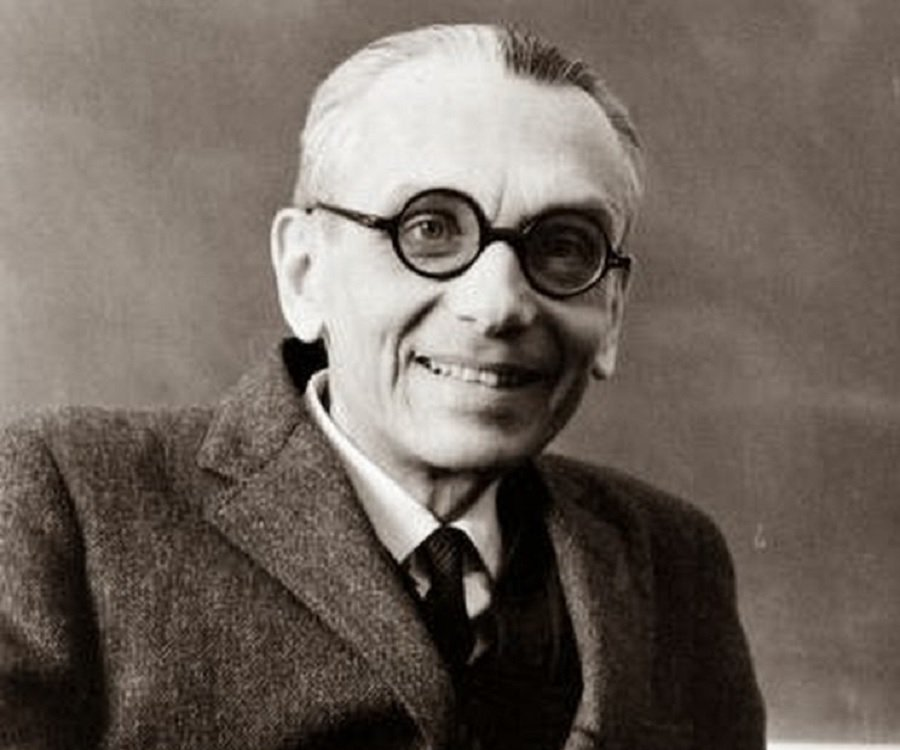
\includegraphics[width=.3\textwidth]{background/godel.jpg}
% % \end{center}

% Consider the following variant of the \HP, the Consistent Guessing Problem
% Given as input a description of a Turing machine $\TM$:
% if the machine $\TM$ accepts on a blank tape, then accept,
% if $\TM$ rejects on a blank tape, then reject, and
% if $TM$ runs forever on a blank tape, then either accept or reject,
% but in any case, halt!

% \margingraphic[l]{0.18\textwidth}{background/pix/rosser.png}{% https://www.math.cornell.edu/m/node/6955
%   \label{fig:rosser}\href{https://en.wikipedia.org/wiki/J._Barkley_Rosser}{J.\@ Barkley Rosser 1987--1989}} % https://www.math.cornell.edu/m/node/6955
% There is no Turing machine to solve the Consistent Guessing Problem.
% Let $P$ be a Turing machine that solves the Consistent Guessing Problem.
% Then we can easily modify $P$ to produce an new Turing machine $Q$ that,
% given as input a description $<\TM>$ of another Turing machine $\TM$:
% rejects if $TM(<\TM>)$ accepts,
% accepts if $\TM<\TM>$ rejects, and
% halts (either accepting or rejecting) if $\TM<\TM>$ runs forever.
% Now run $Q$ on its own description $Q<Q>$.
% If $Q<Q>$ accepts then it rejects; if $Q<Q>$ rejects, then it accepts.
% So the only remaining option is that $Q<Q>$ runs forever, violating the
% third condition.

% From the unsolvability of the Consistent Guessing Problem,
% I claim that Rosser’s Theorem follows.
% For suppose we had a complete and consistent (but not necessarily sound!)
% formal system $F$,
% which was powerful enough to talk about Turing machines.
% Then using $F$ we could solve the Consistent Guessing Problem as follows.
% Given as input a Turing machine description $<\TM>$,
% start enumerating all possible proofs and disproofs of the statement
% ``$\TM$ accepts on a blank tape.''
% Accept as soon as you find a proof, or reject as soon as you find a disproof.

% Because $F$ is complete, you must eventually find either a proof or a disproof
% (and therefore halt, either accepting or rejecting).
% Also, because $F$ is consistent,
% if $\TM$ really rejects then $F$ can't prove that $\TM$ accepts,
% while if $\TM$ really accepts then $F$ can't prove that
% $\TM$ doesn’t accept since in either case the contradiction could be
% discovered in finite time.
% So you'll accept if $\TM$ accepts and reject if $\TM$ rejects.
% But this means that you’re solving Consistent Guessing Problem.

% Just as a beginning programming class encourages a person to think that,
% once you are given a sufficiently detailed specificatino of the problem
% then producing a solution is routine, so also Hilbert and others perceived
% that we could produce an axiom system on which to base Mathematics.
% Then, for any question, with enough smarts we could settle any
% question at issue.

% The \HP{} shows that there are precisely stated problems that cannot be
% solved by an effective procedure.

% http://www.rudyrucker.com/blog/2012/08/01/memories-of-kurt-godel/

% The next form in which Zen expresses itself is the denial of opposites \ldots\,.
% The point is not to be `caught', as the masters would say, in any of the
% four propositions 1.~`It is A'; 2. `It is not-A'.;
% 3. `It is both A and not-A.';
% and 4.~`It is neither A nor not-A.'
% When we manke a negation or an assertion, we are sure to get into one of these
% logical formulas \ldots\,.
% It is in the nature of our logic that any statement we can make is so expressed.
% But Zen thinks that the truth can be reached when it is neither asserted nor
% negated.
% _Essays in Zen Buddhism_
% D.T.Suzuki
% 1949
% Grove Press p. 275
